\bookpart{测度}{Measure}
\label{part:measure}

\BookPartGuide{%
区间有长度，有限集合有元素个数，但许多需要“测量”的集合既不是区间的有限并，也不是有限集。卷一的黎曼积分在这些集合和相应的函数上不够用：它要求被积函数能被有限分割上的阶梯函数逼近，也难以处理极限与积分的交换。本部分从集合的大小出发重新建立积分，再用积分研究局部平均、弱导数以及测度之间的关系。

第~\ref{chap:measure}章规定哪些集合允许测量，以可数可加性定义测度，给出Lebesgue测度等构造，并引入可测函数与简单函数逼近。第~\ref{chap:integration}章由简单函数的加权和定义Lebesgue积分，证明单调收敛、控制收敛与Fubini–Tonelli等换序定理，并说明它与经典积分、微积分基本定理及含参积分的关系。

后三章使用这些工具。第~\ref{chap:smoothing-weak-derivatives}章用卷积做局部平均，构造光滑逼近，再用测试函数的积分恒等式定义弱导数。第~\ref{chap:measure-densities}章比较两个测度的零测集，研究一个测度何时能写成另一个测度的加权积分，即Radon–Nikodym密度。第~\ref{chap:pushforward-measures}章研究质量沿可测映射怎样转移到目标空间，以及目标空间上的积分怎样回到原空间计算。

本部分始终区分“处处”与“几乎处处”、可测与可积、存在密度与可以计算密度。函数空间的范数、完备性与嵌入不在这里展开，它们是第~\ref{part:function-spaces}部分的内容。}

\chapter{测度}
\label{chap:measure}
\label{chap:measure-spaces}
\label{chap:measures}

数一个有限集合有几个元素，量一条线段有多长，称一批货物有多重，回答的都是“这一部分有多大”。这几种测量遵守同一条规则：把对象分成互不相交的几块，整体的大小等于各块大小之和。

困难出现在集合变复杂的时候。区间里的全部有理点该有多长？反复挖去中间三分之一后剩下的点集又有多长？只用有限个区间去逼近，这些问题得不到可靠的回答。

本章把“分开测量、合起来相加”的规则推广到可数次分割。第~\ref{sec:meas-size-additivity}节从计数、长度与Jordan测量出发，用有理点集说明有限覆盖的局限，提出可数可加的要求。第~\ref{sec:meas-measure-spaces}节把“哪些集合允许测量”与“怎样赋予大小”分开，建立$\sigma$代数、测度与完备化。第~\ref{sec:meas-construction}节回答测度从哪里来：由覆盖费用得到外测度，再从简单集合上的赋值延拓出实轴上的Lebesgue测度与Stieltjes测度。

后两节为下一章作准备。第~\ref{sec:meas-signed}节允许测度取负值，用正集与负集把有符号测度拆成两个普通测度之差，并用全变差记录正负两方面的总量。第~\ref{sec:meas-measurable-maps}节用原像定义可测映射与可测函数，证明常见运算和可数极限保持可测性，再用只取有限个值的简单函数从下方逼近非负可测函数。这一逼近正是第~\ref{chap:integration}章定义积分的出发点。

本章只用集合运算、可数性与级数，不使用积分。两个测度之间的比较，以及一个测度能否写成另一个测度的加权积分，留到第~\ref{chap:measure-densities}章；沿可测映射把质量搬到另一个空间的推前测度，留到第~\ref{chap:pushforward-measures}章。

\section{集合大小与可加性}
\label{sec:meas-size-additivity}

测度要推广的是我们已经会做的几件事：数有限集合的元素，量区间的长度，算矩形的面积与体积。本节先从这些测量中提取共同的相加规则，再用有限个矩形从内外两侧逼近一般集合，得到Jordan测量。有理点集的例子将说明，只允许有限个矩形会给某些稀疏的集合不合理的大小；改用可数个区间后，问题转化为一项新的要求：测量规则要对可数运算封闭，并对可数分割可加。

\subsection{计数、长度与体积}
\label{sec:meas-count-length-volume}

\paragraph{计数与加权计数}
对有限集合$A$，用$\#A$表示它的元素个数。若$A$与$B$不相交，合并后每个元素恰好被数一次，所以$\#(A\cup B)=\#A+\#B$。更一般地，给有限集合$X$的每个点$x$配一个非负权重$w_x$，令$A\subseteq X$的大小为$\sum_{x\in A}w_x$。不相交集合合并时，大小仍是两部分之和。权重全取$1$时就是计数；权重不同时，它可以表示质量、费用或频率。

图~\ref{fig:meas-count-length}(a)中$X=\{1,2,3,4,5\}$，权重依次为$0.5,1,2,0.5,1$。分组$A=\{1,2,3\}$、$B=\{4,5\}$后，$A$有$3$个元素、总权重$3.5$，$B$有$2$个元素、总权重$1.5$。整体的个数$5=3+2$，总权重$5=3.5+1.5$。两种大小的数值不同，却遵守同一条规则：不交的部分相加得到整体。

\paragraph{区间长度与矩形体积}
实轴上的区间无法逐个数元素。对端点为$a\leq b$的区间，不论端点是否属于它，规定长度为$b-a$，记作$\ell$。在$\mathbb R^d$中，各边与坐标轴平行的\term{矩形}（rectangle）$R=I_1\times\cdots\times I_d$由$d$个区间相乘得到，规定它的体积为$\lvert R\rvert=\ell(I_1)\cdots\ell(I_d)$。$d=2$时这是面积，$d=1$时回到长度。

长度不是计数的推广。任意两个非退化区间都与$\mathbb R$等势，按元素个数无法区分$[0,1]$与$[0,2]$，长度却分别为$1$和$2$（等势的讨论可参考\BookChapterRef{chap:cardinality}{卷一第3章“基数”}）。所以计数与长度是两种不同的赋值：前者数元素，后者量集合在实轴上占据的范围。无限集合不能笼统地说“一样大”，要先说明用哪一种赋值。

\paragraph{有限个不交矩形的体积}
设$E$是有限个两两不交矩形$R_1,\dots,R_m$的并，自然规定$\lvert E\rvert=\sum_{k=1}^m\lvert R_k\rvert$。同一个$E$往往有多种拆法，这个定义要有意义，必须先说明结果与拆法无关。先看一维：一个区间被切点$a=t_0<t_1<\dots<t_r=b$分开后，小区间长度之和$\sum_j(t_j-t_{j-1})$逐项相消，等于$b-a$。

对两种拆法，取它们全部的端点，从小到大排列，就得到两种拆法的\emph{共同细分}。每种拆法中的每个区间都恰好是若干细分小区间之并，所以两种长度和都等于细分小区间的长度和。$d$维时，在每个坐标方向上取全部边的端点，得到一张网格；每个矩形是若干网格小块之并，体积等于这些小块体积之和，因为乘积$\prod_i\ell(I_i)$对每个因子的切分都可加。于是两种拆法给出同一个总体积。

图~\ref{fig:meas-count-length}(b)中$E=[0,2)\cup[3,4)$。第一种拆法为$[0,1.5),[1.5,2),[3,4)$，长度和为$1.5+0.5+1=3$；第二种为$[0,0.5),[0.5,2),[3,3.5),[3.5,4)$，长度和为$0.5+1.5+0.5+0.5=3$。共同细分的切点是$0,0.5,1.5,2,3,3.5,4$，两种拆法都由这些小区间拼成，总长度相同。

\begin{figure}[!htbp]
  \centering
  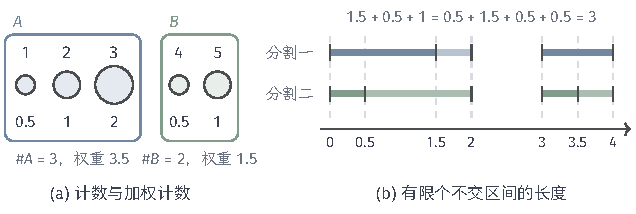
\includegraphics[width=107.6mm]{figures/02-abstract-mathematics/01-metric-and-measure/tikz/c2-count-length/figure.pdf}
  \caption{计数、加权计数与长度遵守同一条不交相加规则。(a)五个点按权重画成大小不同的圆，分成$A=\{1,2,3\}$与$B=\{4,5\}$后，个数$3+2=5$，总权重$3.5+1.5=5$；(b)集合$E=[0,2)\cup[3,4)$的两种不交区间分割，灰色竖线是共同细分的切点，两种分割的长度和都等于$3$。}
  \label{fig:meas-count-length}
\end{figure}

\paragraph{可数拆分时应保持的规则}
上面的可加性只涉及有限个矩形。分析中还会遇到可数拆分。例如
\[
 [0,1)=\bigcup_{k\geq1}\bigl[1-2^{1-k},\,1-2^{-k}\bigr),
\]
这些区间两两不交，长度依次为$\tfrac12,\tfrac14,\tfrac18,\dots$，级数和为$1$，恰好等于$[0,1)$的长度。我们希望这条规则对一切可数拆分都成立：整体长度等于各部分长度的级数和。这不能从有限可加性直接推出，因为有限个区间的拼接只能处理有限个部分。

规则也不能推广到任意多个部分。$[0,1]$是全部单点$\{x\}$之并，每个单点长度为$0$，而“$0$的不可数和”没有定义；若把它理解为$0$，就会得到$[0,1]$的长度为$0$的荒谬结论。所以“有限”与“可数”之间有一条要守住的界线：可数拆分应当保持可加，不可数拆分不作要求。后面建立的测度正是按这条界线设计的。

\subsection{Jordan测量}
\label{sec:meas-jordan}

有限个不交矩形的并只是很少一部分集合。对更一般的有界集合，自然的想法是从里面和外面同时用这类简单集合去逼近，卷二定义区域积分时用的正是这种方法（可参考\BookChapterRef{chap:region-integrals}{卷二第21章“区域积分”}）。下面把有限个有界矩形的并称为\term{初等集合}（elementary set）。它总能改写成有限个不交矩形的并，所以上一小节的体积对它有定义。

\paragraph{内外逼近}
初等集合的体积对包含关系单调。若初等集合$P\subseteq Q$，则$Q\setminus P$仍是初等集合，于是$\lvert P\rvert\leq\lvert P\rvert+\lvert Q\setminus P\rvert=\lvert Q\rvert$。由此可以比较任意一个内部逼近与任意一个外部逼近。

\begin{definition}[Jordan测量]
\label{def:meas-jordan}
设$E\subseteq\mathbb R^d$有界。称
\[
 \begin{aligned}
  J_*(E)&=\sup\{\lvert P\rvert:P\text{为初等集合},\ P\subseteq E\},\\
  J^*(E)&=\inf\{\lvert Q\rvert:Q\text{为初等集合},\ E\subseteq Q\}
 \end{aligned}
\]
分别为$E$的\term{Jordan内测量}（Jordan inner content）与\term{Jordan外测量}（Jordan outer content），其中空集作为初等集合体积为$0$。若$J_*(E)=J^*(E)$，称$E$是\term{Jordan可测}（Jordan measurable）的，公共值记为$J(E)$，称为$E$的\term{Jordan测量}（Jordan content）。
\end{definition}

任取内部初等集合$P\subseteq E$与外部初等集合$Q\supseteq E$，有$P\subseteq Q$，所以$\lvert P\rvert\leq\lvert Q\rvert$，从而总有$J_*(E)\leq J^*(E)$。Jordan可测的意思是两侧能夹逼到同一个数。

\paragraph{边界判据}
两侧逼近之差来自同时接触$E$与$E$外部的那些矩形，所以能否夹逼取决于边界。卷二证明了：有界集合$E$是Jordan可测的，当且仅当它的边界$\partial E$能被有限个总体积任意小的矩形覆盖。直观地说，取一张很细的网格，含于$E$的小块给出内部逼近，与$E$相交的小块给出外部逼近，两者只差与边界相交的小块。

这个判据把问题变成了一个覆盖问题：边界能否用有限个矩形以任意小的总体积盖住。圆盘、多边形等边界光滑或分段光滑的集合都满足它。下面两个一维例子分别说明有限覆盖能做到什么、做不到什么。

\paragraph{有限覆盖可以处理的无限集合}
取$E=\{1/n:n\geq1\}\subseteq\mathbb R$。它不含非退化区间，内测量为$0$。对任意正整数$N$与$\varepsilon>0$，用一个区间$[0,1/N]$盖住$n\geq N$的全部点，再用长度各为$\varepsilon/N$的小区间盖住$1,\tfrac12,\dots,\tfrac1{N-1}$。外部初等集合的总长度不超过$1/N+\varepsilon$，令$N\to\infty$、$\varepsilon\to0$得$J^*(E)=0$。

所以$E$是Jordan可测的，测量为$0$。这里要分清两种“有限”：$E$的元素有无限多个，用来逼近的区间却只有有限个。有限个区间能盖住无限多个点，前提是这些点聚集在少数位置附近；本例中它们聚向$0$，一个短区间就能接住几乎全部的点。

\paragraph{有理点集的反例}
取$E=\mathbb Q\cap[0,1]$。任何非退化区间都含无理数，所以含于$E$的初等集合只能由单点组成，$J_*(E)=0$。另一方面，设初等集合$Q\supseteq E$由区间$I_1,\dots,I_m$组成。把每个$I_k$换成闭包$\overline{I_k}$，长度不变，而$\bigcup_k\overline{I_k}$是含$E$的闭集。$E$在$[0,1]$中稠密，这个闭集必须含$[0,1]$，所以$\lvert Q\rvert\geq1$。$[0,1]$本身是外部初等集合，故$J^*(E)=1$。

内外测量分别为$0$与$1$，$E$不是Jordan可测的。问题出在有限覆盖：有理点到处都是，有限个区间要盖住它们，就不得不连同中间的全部无理数一起盖住。用边界判据看也是一样：$E$的边界是整个$[0,1]$，不能用总长度很小的有限个区间盖住。

\paragraph{改用可数覆盖}
如果允许可数个区间，情况完全不同。把$E$中的点排成一列$q_1,q_2,\dots$。给定$\varepsilon>0$，用长度为$\varepsilon2^{-k}$、以$q_k$为中心的开区间盖住$q_k$。这些区间盖住了$E$，长度总和为$\sum_{k\geq1}\varepsilon2^{-k}=\varepsilon$。图~\ref{fig:meas-jordan-rationals}对比了两种覆盖：有限覆盖必须铺满$[0,1]$，可数覆盖的区间越来越短，总长度可以任意小。在可数覆盖之下，有理点集的大小应当是$0$。

\begin{figure}[!htbp]
  \centering
  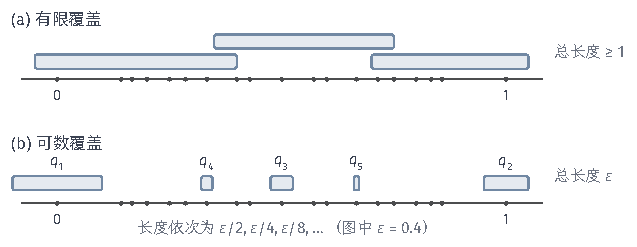
\includegraphics[width=107.8mm]{figures/02-abstract-mathematics/01-metric-and-measure/tikz/c2-jordan-rationals/figure.pdf}
  \caption{用区间覆盖$[0,1]$中的有理点。(a)有限个区间要盖住稠密的有理点，闭包后必须铺满$[0,1]$，总长度不小于$1$；(b)按排列顺序给第$k$个有理点$q_k$分配长度$\varepsilon2^{-k}$的区间，图中只画出前五个，长度依次减半，总长度为$\varepsilon$。}
  \label{fig:meas-jordan-rationals}
\end{figure}

\paragraph{需要重新建立的测量规则}
有理点集还暴露了Jordan测量的另一个缺陷。每个单点都Jordan可测且测量为$0$，它们的可数并$E$却不Jordan可测，所以Jordan可测集合族对可数并不封闭。而分析中处处需要可数运算：一列集合取并或取交，用逐步逼近得到的集合列求极限，把一个集合分成可数个部分。

由此提出两项要求。第一，允许测量的集合族应当对补集和可数并封闭，从而对可数交也封闭。第二，若一个集合被分成可数个不交的可测部分，整体的大小应等于各部分大小的级数和。注意我们没有要求“所有集合都可测”：第一项只规定集合族要有的封闭性，它究竟包含哪些集合，要在构造中确定。下一节先把这两项要求写成定义，满足它们并与长度一致的测量是否存在，由第~\ref{sec:meas-construction}节回答。

\section{测度空间}
\label{sec:meas-measure-spaces}

上一节的两项要求针对两个不同的对象：一项限定哪些集合允许测量，另一项规定怎样给这些集合赋予大小。本节把它们分开建立。

我们先用$\sigma$代数描述允许测量的集合族，并在度量空间上由开集得到Borel集；再在其上定义可数可加的测度，推出比较集合与取极限的规则；最后讨论零测集，说明忽略哪些点不会改变测量，以及怎样把零测集的子集也纳入可测范围。

\subsection{$\sigma$代数}
\label{sec:meas-sigma-algebras}

\paragraph{能够区分哪些集合}
设$X=\{1,2,3,4\}$。若允许测量全部$16$个子集，就能单独询问每个点的大小。若我们只知道每个点属于$\{1,2\}$还是$\{3,4\}$，能够回答的就只有下面四个集合：
\[
 \varnothing,\quad\{1,2\},\quad\{3,4\},\quad X.
\]
单点$\{1\}$这时无法单独测量。两种集合族的底集相同，区分能力不同。

可以把一个集合族看成一份“允许提问的清单”：清单上的集合，才能问它有多大。无论清单选哪一份，都应满足上一节的封闭性要求：能问“在$A$中吗”，就能问“不在$A$中吗”；能问一列集合中的每一个，就能问“至少在其中一个中吗”。把这两条写下来，就是下面的定义。

\begin{definition}[$\sigma$代数]
\label{def:meas-sigma-algebra}
设$X$是集合，$\mathcal A$是$X$的一族子集。若
\begin{enumerate}
 \item $X\in\mathcal A$；
 \item $A\in\mathcal A$蕴含$X\setminus A\in\mathcal A$；
 \item $A_1,A_2,\dots\in\mathcal A$蕴含$\bigcup_{n\geq1}A_n\in\mathcal A$，
\end{enumerate}
则称$\mathcal A$为$X$上的一个\term{$\sigma$代数}（sigma-algebra），称$(X,\mathcal A)$为\term{可测空间}（measurable space），称$\mathcal A$中的集合为\term{可测集合}（measurable set）。
\end{definition}

定义只列出补集与可数并，其他运算由它们得到。由第1、2条，$\varnothing=X\setminus X\in\mathcal A$；在第3条中从某项起全取$\varnothing$，得到有限并封闭。可数交由De Morgan律化为补集与并：
\[
 \bigcap_{n\geq1}A_n=X\setminus\bigcup_{n\geq1}(X\setminus A_n).
\]

差集$A\setminus B=A\cap(X\setminus B)$也属于$\mathcal A$。所以从可测集合出发，经可数次补、并、交、差得到的集合仍然可测。开头的两种清单都满足这些条件：幂集$\mathcal P(X)$含全部子集；四个集合$\varnothing,\{1,2\},\{3,4\},X$中任一个的补集、任意几个的并也都在其中。

\paragraph{生成的$\sigma$代数}
实际问题中，我们通常只点名少数必须能测量的集合，例如区间或若干类别，希望由它们补齐其余集合。给定$X$的一族子集$\mathcal C$，包含$\mathcal C$的$\sigma$代数至少有幂集一个。令$\sigma(\mathcal C)$为所有包含$\mathcal C$的$\sigma$代数之交，称为$\mathcal C$\term{生成的$\sigma$代数}（generated sigma-algebra）。

这个交确实是$\sigma$代数：每个参与求交的$\sigma$代数都含$X$，并对补集、可数并封闭；交集中的元素同时属于它们全体，运算结果也同时属于它们全体。它包含$\mathcal C$，又包含于任何包含$\mathcal C$的$\sigma$代数，所以是其中最小的一个。

这与线性代数中“由一组向量张成的子空间”很像：张成的子空间是包含这组向量的最小子空间，也可以写成所有包含它们的子空间之交。那里的运算是线性组合，这里的运算是补集和可数并。不同之处在于，张成的子空间有“全体有限线性组合”这样的显式表达，而$\sigma(\mathcal C)$一般写不出这样的清单，只能用封闭性来描述。

\begin{example}[有限分组生成的$\sigma$代数]
\label{ex:meas-partition-sigma}
在$X=\{1,2,3,4\}$上取$\mathcal C=\{\{1\},\{2\}\}$。生成的$\sigma$代数必须含$\{1\}$、$\{2\}$，以及
\[
 X\setminus(\{1\}\cup\{2\})=\{3,4\}.
\]
于是它含分组$\{1\},\{2\},\{3,4\}$中任意几组的并，共$2^3=8$个集合。这$8$个集合对补集和并已经封闭，所以它们就是$\sigma(\mathcal C)$，而$\{3\}$不在其中。
\end{example}

图~\ref{fig:meas-partition-sigma}比较了三种分组。有限集合上的$\sigma$代数都由某个分组决定：可测集合恰是若干组之并，组分得越细，可以单独测量的集合就越多。

\begin{BookInlineFigure}
  \centering
  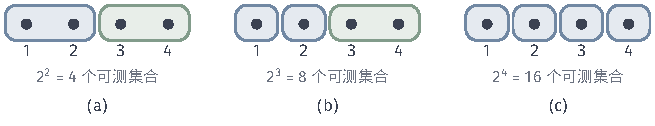
\includegraphics[width=110.938mm]{figures/04-spaces-measures-and-geometry/02-measure/tikz/meas-sigma-algebra-partition/figure.pdf}
  \caption{四点集合$X=\{1,2,3,4\}$上由分组生成的$\sigma$代数。每个色块是一组，可测集合恰是若干组之并。(a)分成$\{1,2\},\{3,4\}$两组；(b)分成$\{1\},\{2\},\{3,4\}$三组；(c)每点自成一组，得到全部子集。}
  \label{fig:meas-partition-sigma}
\end{BookInlineFigure}

生成操作补齐的只是可数运算的封闭性，未必得到所有希望测量的集合。在$\mathbb R$上取全体单点组成的族$\mathcal C$，令$\mathcal D$为可数集合与补集可数的集合的全体。

$\mathcal D$含$\mathbb R$，对补集封闭。对一列$\mathcal D$中的集合，若都可数，则并可数；若其中有一个补集可数，则并的补集包含于它的补集，也可数。所以$\mathcal D$是含全部单点的$\sigma$代数，于是$\sigma(\mathcal C)\subseteq\mathcal D$。

而$[0,1]$与它的补集都不可数，所以$[0,1]\notin\mathcal D$。可见单点生成的$\sigma$代数不含任何非退化区间；要测量区间，生成族里必须直接放入区间或开集。

\paragraph{Borel集}
在度量空间中已经有一族自然的集合：开集。第~\ref{chap:topological-spaces}章用开集表达连续、收敛与紧性，第~\ref{chap:metric-spaces}章又用开球刻画度量空间的开集。把开集作为生成族，得到的可测范围就与这些结构相容。

\begin{definition}[Borel $\sigma$代数]
\label{def:meas-borel}
设$X$是度量空间（更一般地，拓扑空间）。由全体开集生成的$\sigma$代数称为$X$的\term{Borel $\sigma$代数}（Borel sigma-algebra），记作$\mathcal B(X)$，其中的集合称为\term{Borel集}（Borel set）。
\end{definition}

开集的补集是闭集，所以闭集都是Borel集；可数个闭集的并、可数个开集的交也是Borel集。例如$\mathbb Q$是可数个闭集$\{q\}$的并，$[0,1)=\bigcap_{n\geq1}(-1/n,1)$是可数个开集的交，二者都是Borel集。

要强调的是，$\mathcal B(X)$只规定了哪些集合允许测量，并没有规定任何集合的大小。同一个Borel结构上可以放置长度、点质量或它们的组合等不同的测度。

\paragraph{实轴上的生成族}
直接处理全部开集并不方便。下面说明较小的区间族已经够用，关键是把任意开集写成可数个区间的并。

\begin{lemma}[开集的有理区间表示]
\label{lem:meas-open-rational-intervals}
$\mathbb R$中每个开集$U$都是有理端点开区间的可数并。
\end{lemma}

\begin{proof}
任取$x\in U$。因为$U$是开集，存在$r>0$使$(x-r,x+r)\subseteq U$。有理数在实轴上稠密，可取有理数$p,q$满足
\[
 x-r<p<x<q<x+r,
\]
于是$x\in(p,q)\subseteq U$。

所以$U$等于所有含于$U$的有理端点开区间$(p,q)$之并。这样的区间由有序对$(p,q)\in\mathbb Q\times\mathbb Q$确定，而$\mathbb Q\times\mathbb Q$可数，所以这是可数并。
\end{proof}

\begin{theorem}[$\mathcal B(\mathbb R)$的生成族]
\label{thm:meas-borel-generators}
下列每一族集合都生成$\mathcal B(\mathbb R)$：(1)全体开区间$(a,b)$；(2)全体半直线$(a,+\infty)$；(3)全体半直线$(-\infty,a]$；(4)全体左开右闭区间$(a,b]$。在(2)(3)中只取有理数$a$也够用。
\end{theorem}

\begin{proof}
各族中的集合都是开集、闭集或二者之交，属于$\mathcal B(\mathbb R)$，所以它们生成的$\sigma$代数都含于$\mathcal B(\mathbb R)$。反方向只需说明每个开集属于各族生成的$\sigma$代数。对族(1)，这就是引理~\ref{lem:meas-open-rational-intervals}。

其余各族都能经可数运算得到开区间。先看半直线。取有理数列$p_n$严格递减趋于$a$，则
\[
 (a,+\infty)=\bigcup_n(p_n,+\infty),
\]
所以有理端点的半直线已能生成族(2)。又因$(-\infty,a]$的补集是$(a,+\infty)$，族(3)与族(2)生成同一个$\sigma$代数。

再看半开区间与开区间。由下面两个等式：
\[
 (a,b]=(-\infty,b]\setminus(-\infty,a],\qquad
 (a,b)=\bigcup_{n}\,(a,\,b-1/n]
\]
（后式中$n$取使$b-1/n>a$的整数），可知开区间属于族(3)或族(4)生成的$\sigma$代数。
\end{proof}

同样的论证在$\mathbb R^d$中成立：每个开集是可数个有理顶点开矩形之并，所以开矩形生成$\mathcal B(\mathbb R^d)$；把开矩形写成左开右闭矩形的可数并，可知左开右闭矩形$\prod_i(a_i,b_i]$也生成$\mathcal B(\mathbb R^d)$。

\subsection{测度及其基本性质}
\label{sec:meas-measures}

\paragraph{测度的定义}
可测范围确定以后，要给每个可测集合配一个非负的大小，并要求可数可加。允许取值$+\infty$，因为整条实轴的长度、无限集合的元素个数都没有有限的值。在$[0,+\infty]$中约定$a+(+\infty)=+\infty$，非负项级数的和是部分和的上确界，可以为$+\infty$。

\begin{definition}[测度]
\label{def:meas-measure}
设$(X,\mathcal A)$是可测空间。映射$\mu:\mathcal A\to[0,+\infty]$若满足$\mu(\varnothing)=0$，并且对两两不交的$A_1,A_2,\dots\in\mathcal A$有
\begin{equation}
 \mu\Bigl(\bigcup_{n\geq1}A_n\Bigr)=\sum_{n\geq1}\mu(A_n),
 \label{eq:meas-countable-additivity}
\end{equation}
则称$\mu$为$(X,\mathcal A)$上的\term{测度}（measure），称$(X,\mathcal A,\mu)$为\term{测度空间}（measure space）。式~\eqref{eq:meas-countable-additivity}称为\term{可数可加性}（countable additivity）。
\end{definition}

非负项级数的和与求和次序无关，所以式~\eqref{eq:meas-countable-additivity}右端不依赖集合的排列方式，这与左端的并集不依赖排列相一致。条件$\mu(\varnothing)=0$排除了一切集合都取$+\infty$的平凡赋值；若某个$A$满足$\mu(A)<+\infty$，取$A_1=A$、其余为空集，由式~\eqref{eq:meas-countable-additivity}也能推出它。

\paragraph{计数测度与点质量}
在任意可测空间上，令$\mu(A)=\#A$（$A$为无限集时取$+\infty$），称为\term{计数测度}（counting measure）。核对可数可加性：若不交的$A_n$中只有有限个非空且都是有限集，两边都是元素总数；若某个$A_n$无限，或有无限多个$A_n$非空，并集无限，右边的级数也发散到$+\infty$。

固定$x\in X$，规定
\[
 \delta_x(A)=\begin{cases}1,&x\in A,\\0,&x\notin A,\end{cases}
\]
称为点$x$处的\term{Dirac测度}（Dirac measure）。不交集合列中至多一个含$x$，所以可数可加性成立。

这个定义只读取可测集合$A$是否含$x$，并不要求单点$\{x\}$本身可测。例如在$\mathcal A=\{\varnothing,\{1,2\},\{3,4\},X\}$上，$\delta_1$给$\{1,2\}$赋值$1$，给$\{3,4\}$赋值$0$，尽管$\{1\}$不可测。

把可数个点质量按非负权重相加，得到$\mu=\sum_kw_k\delta_{x_k}$，即$\mu(A)=\sum_{k:x_k\in A}w_k$。它推广了上一节的加权计数。核对可数可加性时要交换两重求和：
\[
 \sum_n\sum_kw_k\delta_{x_k}(A_n)=\sum_k\sum_nw_k\delta_{x_k}(A_n).
\]
非负二重级数的两种累次求和相等，因为任意有限部分和都不超过另一种次序的总和，令有限范围扩大即得两个方向的不等式。

例如在$\mathbb N=\{1,2,\dots\}$上取$\mu=\sum_n2^{-n}\delta_n$。总量是
\[
 \mu(\mathbb N)=\sum_{n\geq1}2^{-n}=1,
\]
偶数集的测度是
\[
 \mu(\{2,4,6,\dots\})=\sum_{m\geq1}2^{-2m}=\sum_{m\geq1}4^{-m}=\frac13.
\]

\paragraph{有限性条件}
测度可以整体取$+\infty$，但不同测度“无限”的方式差别很大，后面一些结论要区分它们。

\begin{definition}[有限测度、概率测度与$\sigma$有限测度]
\label{def:meas-finiteness}
设$(X,\mathcal A,\mu)$是测度空间。若$\mu(X)<+\infty$，称$\mu$为\term{有限测度}（finite measure）；若$\mu(X)=1$，称$\mu$为\term{概率测度}（probability measure）；若存在$X_1,X_2,\dots\in\mathcal A$使$X=\bigcup_nX_n$且每个$\mu(X_n)<+\infty$，称$\mu$为\term{$\sigma$有限测度}（sigma-finite measure）。
\end{definition}

有限测度都是$\sigma$有限的。$\mathbb N$上的计数测度总量为$+\infty$，但$\mathbb N=\bigcup_n\{n\}$且每个单点计数为$1$，所以它$\sigma$有限：整体无限，却能切成可数个有限的片。

$\mathbb R$上以全部子集为可测范围的计数测度不是$\sigma$有限的。若$\mathbb R=\bigcup_nX_n$且每个$X_n$都是有限集，$\mathbb R$就可数了，这是矛盾。唯一性定理和乘积测度需要$\sigma$有限条件，下面的基本性质不需要；我们在每处单独声明，不把它当作统一假设。

\paragraph{基本性质}
可数可加性只直接说到不交集合。比较有包含关系的集合、处理互相重叠的集合、对集合列取极限，都要先把集合拆成不交的部分。

\begin{theorem}[测度的基本性质]
\label{thm:meas-basic-properties}
设$(X,\mathcal A,\mu)$是测度空间，以下集合都属于$\mathcal A$。
\begin{enumerate}
 \item 有限可加性：若$A_1,\dots,A_m$两两不交，则
 \begin{equation}
  \mu\Bigl(\bigcup_{k=1}^mA_k\Bigr)=\sum_{k=1}^m\mu(A_k).
  \label{eq:meas-finite-additive}
 \end{equation}
 \item 单调性：$A\subseteq B$蕴含$\mu(A)\leq\mu(B)$；若还有$\mu(A)<+\infty$，则
 \begin{equation}
  \mu(B\setminus A)=\mu(B)-\mu(A).
  \label{eq:meas-monotone-difference}
 \end{equation}
 \item 可数次可加性：$A_n$不必两两不交，都有
 \begin{equation}
  \mu\Bigl(\bigcup_nA_n\Bigr)\leq\sum_n\mu(A_n).
  \label{eq:meas-countable-subadditive}
 \end{equation}
 \item 从下连续性：若$A_1\subseteq A_2\subseteq\cdots$，则
 \begin{equation}
  \mu\Bigl(\bigcup_nA_n\Bigr)=\lim_{n\to\infty}\mu(A_n).
  \label{eq:meas-continuity-below}
 \end{equation}
 \item 从上连续性：若$A_1\supseteq A_2\supseteq\cdots$且$\mu(A_1)<+\infty$，则
 \begin{equation}
  \mu\Bigl(\bigcap_nA_n\Bigr)=\lim_{n\to\infty}\mu(A_n).
  \label{eq:meas-continuity-above}
 \end{equation}
\end{enumerate}
\end{theorem}

\begin{proof}
第1条在可数可加性中令$A_n=\varnothing$（$n>m$）即得。

对第2条，$B=A\cup(B\setminus A)$是不交并，由第1条
\[
 \mu(B)=\mu(A)+\mu(B\setminus A)\geq\mu(A).
\]
当$\mu(A)$有限时，两边可以减去$\mu(A)$，得到差集的公式。

对第3条，先把重叠的部分去掉：令$B_1=A_1$，$B_n=A_n\setminus\bigcup_{k<n}A_k$。这些$B_n$两两不交，$B_n\subseteq A_n$，并且$\bigcup_nB_n=\bigcup_nA_n$。由可数可加性与单调性，
\[
 \mu\Bigl(\bigcup_nA_n\Bigr)=\sum_n\mu(B_n)\leq\sum_n\mu(A_n).
\]

对第4条，令$A_0=\varnothing$，$D_n=A_n\setminus A_{n-1}$。这些相邻差集两两不交，$A_n=\bigcup_{k\leq n}D_k$，$\bigcup_nA_n=\bigcup_kD_k$，所以
\[
 \mu\Bigl(\bigcup_nA_n\Bigr)=\sum_{k=1}^{\infty}\mu(D_k)
 =\lim_{n\to\infty}\sum_{k=1}^n\mu(D_k)=\lim_{n\to\infty}\mu(A_n).
\]

对第5条，令$C_n=A_1\setminus A_n$，它们递增，并为$A_1\setminus\bigcap_nA_n$。由第4条，
\[
 \mu\Bigl(A_1\setminus\bigcap_nA_n\Bigr)=\lim_{n\to\infty}\mu(A_1\setminus A_n).
\]
因为$\mu(A_1)<+\infty$，第2条允许把两边写成差：
\[
 \mu(A_1)-\mu\Bigl(\bigcap_nA_n\Bigr)=\mu(A_1)-\lim_{n\to\infty}\mu(A_n).
\]
消去有限数$\mu(A_1)$，即得结论。
\end{proof}

这两条连续性可以用同一个测度手算。在$\mathbb N$上取$\mu=\sum_n2^{-n}\delta_n$，令递增列$A_n=\{1,\dots,n\}$，递减列$B_n=\{n,n+1,\dots\}$。则
\[
 \mu(A_n)=1-2^{-n}\to1=\mu(\mathbb N),\qquad
 \mu(B_n)=2^{1-n}\to0=\mu(\varnothing).
\]
递增时测度从下面爬向极限集合的测度，递减时测度从上面落到极限集合的测度，两者都正好对上式~\eqref{eq:meas-continuity-below}与式~\eqref{eq:meas-continuity-above}。

第5条中的有限性条件不能省略。在$\mathbb N$上取计数测度与尾集$A_n=\{n,n+1,\dots\}$。每个$A_n$都是无限集，$\mu(A_n)=+\infty$，而$\bigcap_nA_n=\varnothing$，测度为$0$。证明失效的位置是“两边减去$\mu(A_1)$”，因为$+\infty-(+\infty)$没有意义。

只要从某项起$\mu(A_n)$有限，把这一项当作首项即可应用第5条。所以从下连续性无条件成立，从上连续性需要一个有限的起点，两者不能混用。

\paragraph{限制与加权和}
从已有测度得到新测度有几种常用操作。设$E\in\mathcal A$，令$\mu|_E(A)=\mu(A\cap E)$，它仍是$(X,\mathcal A)$上的测度，只保留$E$内的质量。

若$\mu_1,\mu_2,\dots$是测度，$c_k\in[0,+\infty]$，并约定$0\cdot(+\infty)=0$，则$\sum_kc_k\mu_k$也是测度；核对可数可加性时同样只需交换非负二重级数的求和次序。约定$0\cdot(+\infty)=0$保证系数为零的项对任何集合都贡献零，不会产生没有定义的乘积。

\subsection{测度的完备化}
\label{sec:meas-completion}

\paragraph{零测集与几乎处处}
测量中常有一些例外点：它们存在，但质量为零，不影响任何集合的大小。我们希望能说“除去一个可以忽略的集合，某性质成立”。

\begin{definition}[零测集与几乎处处]
\label{def:meas-null-set}
设$(X,\mathcal A,\mu)$是测度空间。满足$\mu(N)=0$的$N\in\mathcal A$称为$\mu$-\term{零测集}（null set）。若使某个关于点的性质不成立的点全体包含于某个$\mu$-零测集，称该性质$\mu$-\term{几乎处处}（almost everywhere）成立，记作$\mu$-a.e.。
\end{definition}

“逐点成立”要求性质在每一点都对，“几乎处处成立”允许它在一个零测集上失败。定义只要求失败点集\emph{包含于}一个零测集，因为失败点集本身未必可测。

几乎处处总是相对于当前测度而言的。在$X=\{0,1\}$与$\mathcal A=\mathcal P(X)$上，$\{1\}$是$\delta_0$的零测集，却承载$\delta_1$的全部质量。于是“函数在点$1$以外取零”对$\delta_0$几乎处处成立，对$\delta_1$不成立，这句话换一个测度就要重新判断。

可数个零测例外可以合并：若$N_1,N_2,\dots$都是零测集，由可数次可加性，
\[
 \mu\Bigl(\bigcup_nN_n\Bigr)\leq\sum_n\mu(N_n)=0.
\]
所以一列性质若各自几乎处处成立，它们同时几乎处处成立。这一论证依赖可数次可加性，对不可数个零测集不适用；下一节构造长度测度后会看到，$[0,1]$是不可数个长度为零的单点之并，自身长度却为$1$。

\paragraph{零测集的子集}
零测集的子集“更应当”可以忽略，可它不一定可测。在$X=\{1,2,3\}$上取$\mathcal A=\{\varnothing,\{1\},\{2,3\},X\}$与$\mu=\delta_1$，$\{2,3\}$是零测集，它的子集$\{2\}$却不可测，连“$\{2\}$的测度为零”这句话都说不出。

\begin{definition}[完备测度空间]
\label{def:meas-complete}
若测度空间$(X,\mathcal A,\mu)$中每个零测集的每个子集都属于$\mathcal A$，称该测度空间是\term{完备}（complete）的。
\end{definition}

这里的完备与第~\ref{chap:metric-spaces}章度量空间的完备性（Cauchy列收敛）是两个不同的概念，只是同名。不完备的测度空间可以通过补入零测集的子集来修补，关键是补入以后不能改变原有集合的测度。

\begin{theorem}[测度空间的完备化]
\label{thm:meas-completion}
设$(X,\mathcal A,\mu)$是测度空间。令$\overline{\mathcal A}$为形如$A\cup M$的集合全体，其中$A\in\mathcal A$，$M$包含于某个$\mu$-零测集；规定$\overline\mu(A\cup M)=\mu(A)$。则$\overline{\mathcal A}$是包含$\mathcal A$的$\sigma$代数，$\overline\mu$是其上不依赖表示方式的测度，在$\mathcal A$上与$\mu$一致，且$(X,\overline{\mathcal A},\overline\mu)$完备。它称为$(X,\mathcal A,\mu)$的\term{完备化}（completion）。
\end{theorem}

\begin{proof}
先证赋值与表示方式无关。设$A\cup M=A'\cup M'$，其中$M\subseteq N$、$M'\subseteq N'$，$N,N'$是零测集。则$A\subseteq A'\cup N'$，由单调性与次可加性，
\[
 \mu(A)\leq\mu(A')+\mu(N')=\mu(A').
\]
对称地$\mu(A')\leq\mu(A)$，所以$\mu(A)=\mu(A')$。取$M=\varnothing$可知$\mathcal A\subseteq\overline{\mathcal A}$，且$\overline\mu$在$\mathcal A$上等于$\mu$。

再证$\overline{\mathcal A}$是$\sigma$代数。对补集，设$M\subseteq N$，则
\[
 X\setminus(A\cup M)=\bigl((X\setminus A)\setminus N\bigr)\cup\bigl((X\setminus A)\cap(N\setminus M)\bigr),
\]
第一项属于$\mathcal A$，第二项包含于零测集$N$。对可数并，
\[
 \bigcup_n(A_n\cup M_n)=\Bigl(\bigcup_nA_n\Bigr)\cup\Bigl(\bigcup_nM_n\Bigr),
\]
而$\bigcup_nM_n\subseteq\bigcup_nN_n$，后者是零测集。

然后证可数可加性。若$A_n\cup M_n$两两不交，则$A_n$两两不交，于是
\[
 \overline\mu\Bigl(\bigcup_n(A_n\cup M_n)\Bigr)=\mu\Bigl(\bigcup_nA_n\Bigr)
 =\sum_n\mu(A_n)=\sum_n\overline\mu(A_n\cup M_n).
\]

最后证完备性。若$\overline\mu(A\cup M)=0$，则$\mu(A)=0$，$A\cup M\subseteq A\cup N$，后者是$\mu$-零测集。$A\cup M$的任一子集$S$可写成$\varnothing\cup S$，其中$S$包含于零测集$A\cup N$，所以$S\in\overline{\mathcal A}$。
\end{proof}

在上面的例子中，零测集$\{2,3\}$的子集$\{2\}$、$\{3\}$被补入，得到$\overline{\mathcal A}=\mathcal P(X)$，$\overline\mu=\delta_1$。完备化不改变原有集合的测度，只把“包含于零测集”的集合也纳入可测范围并赋值为零。

是否需要完备化取决于问题：讨论零测集上修改函数后的可测性时它很方便，讨论乘积空间的截面时它又会带来额外的例外，这一点在第~\ref{chap:integration}章再说明。

\section{测度的构造}
\label{sec:meas-construction}

上一节规定了测度应满足的规则，并用计数、点质量等例子验证了这些规则可以实现。可是第~\ref{sec:meas-size-additivity}节真正想要的长度测度还没有出现：我们只知道区间的长度，并不知道怎样把它可数可加地推广到$\mathcal B(\mathbb R)$。

本节分三步回答。先把可数覆盖的想法做成外测度，从中选出满足分割可加的集合；再把这条路线抽象成从简单集合族出发的延拓定理，分别回答延拓是否存在、是否唯一；最后用它构造实轴上的Lebesgue测度和Stieltjes测度。

\subsection{外测度}
\label{sec:meas-outer-measure}

\paragraph{覆盖的总费用}
有理点集的例子提示了一种测量方式：用一列简单集合覆盖待测集合，算出覆盖的总费用，再让总费用尽量小。可以把简单集合想成一种按件定价的“包装”，给一个集合算大小，就是问把它完全打包最少要花多少钱。这样得到的量对每个子集都有定义，但它满足的规则比测度少。

\begin{definition}[外测度]
\label{def:meas-outer}
集合$X$上的\term{外测度}（outer measure）是映射$\mu^*:\mathcal P(X)\to[0,+\infty]$，满足：$\mu^*(\varnothing)=0$；$E\subseteq F$蕴含$\mu^*(E)\leq\mu^*(F)$；对任意$E_1,E_2,\dots\subseteq X$，有
\begin{equation}
 \mu^*\Bigl(\bigcup_nE_n\Bigr)\leq\sum_n\mu^*(E_n).
 \label{eq:meas-outer-subadditive}
\end{equation}
\end{definition}

外测度只要求次可加，不要求可加。下面的引理说明，任何一种“简单集合的费用”都能经可数覆盖变成外测度，这就是把局部赋值推广到任意子集的方法。

\begin{lemma}[由覆盖得到外测度]
\label{lem:meas-cover-outer}
设$\mathcal C$是$X$的一族子集，$\varnothing\in\mathcal C$，$\rho:\mathcal C\to[0,+\infty]$满足$\rho(\varnothing)=0$。对$E\subseteq X$令
\begin{equation}
 \mu^*(E)=\inf\Bigl\{\sum_{n\geq1}\rho(C_n):C_n\in\mathcal C,\ E\subseteq\bigcup_{n\geq1}C_n\Bigr\},
 \label{eq:meas-cover-outer}
\end{equation}
没有这样的覆盖时取$+\infty$。则$\mu^*$是外测度。
\end{lemma}

\begin{proof}
取全部$C_n=\varnothing$覆盖空集，得$\mu^*(\varnothing)=0$。若$E\subseteq F$，覆盖$F$的每一列集合也覆盖$E$，下确界取在更大的范围上，故$\mu^*(E)\leq\mu^*(F)$。

对次可加性，不妨设$\sum_n\mu^*(E_n)<+\infty$，任取$\varepsilon>0$。对每个$n$，按下确界的定义选覆盖$E_n$的$C_{n,1},C_{n,2},\dots\in\mathcal C$，使
\[
 \sum_k\rho(C_{n,k})\leq\mu^*(E_n)+\varepsilon2^{-n}.
\]

全体$C_{n,k}$可以排成一列并覆盖$\bigcup_nE_n$，非负项的排列不改变级数和，于是
\[
 \mu^*\Bigl(\bigcup_nE_n\Bigr)\leq\sum_n\sum_k\rho(C_{n,k})
 \leq\sum_n\bigl(\mu^*(E_n)+\varepsilon2^{-n}\bigr)=\sum_n\mu^*(E_n)+\varepsilon.
\]
令$\varepsilon\to0$即得结论。
\end{proof}

外测度能给每个子集赋值，代价是失去可加性。在$X=\{1,2\}$上取$\mathcal C=\{\varnothing,X\}$、$\rho(X)=1$。唯一有效的覆盖是$X$本身，所以
\[
 \mu^*(\{1\})=\mu^*(\{2\})=\mu^*(X)=1.
\]
不交的$\{1\}$与$\{2\}$外测度之和为$2$，它们的并的外测度却是$1$。原因是这份价目表只卖整包，无法把两点分开计价，见图~\ref{fig:meas-carath-cut}(b)。因此要找出外测度在哪些集合上可加。

\paragraph{Carathéodory可测性}
一个集合$A$要“与外测度相容”，应当意味着用$A$去切任何集合都不会多算或少算。图~\ref{fig:meas-carath-cut}(a)画的正是这个检验：拿一个测试集合$E$，用$A$切成两块，比较切开前后的总价。只在一个特定的$E$上检验还不够，下面的判据要求对一切测试集合都成立。

\begin{BookInlineFigure}
  \centering
  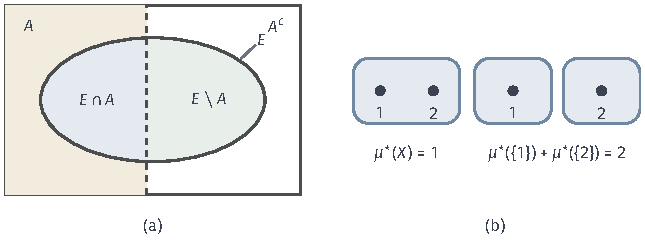
\includegraphics[width=109.238mm]{figures/04-spaces-measures-and-geometry/02-measure/tikz/meas-carath-cut/figure.pdf}
  \caption{Carathéodory判据的含义。(a)测试集合$E$（椭圆）被$A$切成$E\cap A$（蓝）与$E\setminus A$（绿），可测要求两块的外测度之和总等于$\mu^*(E)$；(b)价目表只卖整包$X$时，切开$X=\{1,2\}$迫使每点各付一个整包的价，$\{1\}$不满足判据。}
  \label{fig:meas-carath-cut}
\end{BookInlineFigure}

\begin{definition}[Carathéodory可测]
\label{def:meas-caratheodory-measurable}
设$\mu^*$是$X$上的外测度。若对每个$E\subseteq X$都有
\begin{equation}
 \mu^*(E)=\mu^*(E\cap A)+\mu^*(E\setminus A),
 \label{eq:meas-caratheodory-criterion}
\end{equation}
称$A\subseteq X$为$\mu^*$-\term{Carathéodory可测}（Carathéodory measurable）的。
\end{definition}

由次可加性，“$\leq$”总成立，所以验证时只需证明“$\geq$”，并且只需对$\mu^*(E)<+\infty$的$E$验证。上例中$\{1\}$不满足判据：取$E=X$，右边为$2$，左边为$1$。

再看一个能选出非平凡集合的例子。取$X=\{1,2,3\}$，价目表$\mathcal C=\{\varnothing,\{1\},\{2,3\},X\}$，价格为
\[
 \rho(\{1\})=1,\qquad\rho(\{2,3\})=2,\qquad\rho(X)=3.
\]
点$2$、$3$只能打包购买。由式~\eqref{eq:meas-cover-outer}，单点和两点集的外测度是
\[
 \mu^*(\{1\})=1,\quad \mu^*(\{2\})=\mu^*(\{3\})=\mu^*(\{2,3\})=2,\quad \mu^*(\{1,2\})=3.
\]

检验$A=\{1\}$：取$E=X$，$1+2=3$；取$E=\{2\}$，$0+2=2$；取$E=\{1,2\}$，$1+2=3$，等式都成立，其余$E$同样核对。检验$A=\{2\}$：取$E=\{2,3\}$，右边是$\mu^*(\{2\})+\mu^*(\{3\})=4$，左边是$2$，判据不成立。

逐一检查可知全部可测集是$\varnothing,\{1\},\{2,3\},X$：恰好是价目表上明码标价的那些集合。下面的定理说明，这样选出的集合总是构成$\sigma$代数，外测度在上面可数可加。

\begin{theorem}[Carathéodory定理]
\label{thm:meas-caratheodory}
设$\mu^*$是$X$上的外测度，$\mathcal M$为全体$\mu^*$-Carathéodory可测集。则$\mathcal M$是$\sigma$代数，$\mu^*$在$\mathcal M$上的限制是测度，且$(X,\mathcal M,\mu^*|_{\mathcal M})$完备；特别地，$\mu^*(N)=0$的集合$N$都属于$\mathcal M$。
\end{theorem}

证明分三步：先处理补集与有限并，再控制可数不交并，最后由不交化得到一般的可数并，同时读出可数可加性。

\begin{proof}
\emph{补集与有限并。}判据关于$A$与$X\setminus A$对称，所以$\mathcal M$对补集封闭；$X\in\mathcal M$是因为$\mu^*(\varnothing)=0$。

设$A,B\in\mathcal M$，$E\subseteq X$。先用$A$切$E$，再用$B$切$E\setminus A$，得到
\[
 \mu^*(E)=\mu^*(E\cap A)+\mu^*\bigl((E\setminus A)\cap B\bigr)+\mu^*\bigl(E\setminus(A\cup B)\bigr).
\]
把前两项涉及的两块并起来，就是$A\cup B$切出的部分：
\[
 E\cap(A\cup B)=(E\cap A)\cup\bigl((E\setminus A)\cap B\bigr).
\]
次可加性说明前两项之和不小于$\mu^*(E\cap(A\cup B))$，于是
\[
 \mu^*(E)\geq\mu^*\bigl(E\cap(A\cup B)\bigr)+\mu^*\bigl(E\setminus(A\cup B)\bigr).
\]
这就是$A\cup B$的判据。于是$\mathcal M$对有限并、有限交与差都封闭。

\emph{可数不交并。}设$A_1,A_2,\dots\in\mathcal M$两两不交，$B_n=\bigcup_{k\leq n}A_k$，$B=\bigcup_kA_k$。用$A_n$切测试集合$E\cap B_n$，因$A_n$与$B_{n-1}$不交，得
\[
 \mu^*(E\cap B_n)=\mu^*(E\cap A_n)+\mu^*(E\cap B_{n-1}).
\]
对$n$归纳，得到
\[
 \mu^*(E\cap B_n)=\sum_{k\leq n}\mu^*(E\cap A_k).
\]

再用$B_n\in\mathcal M$切$E$，并由$E\setminus B_n\supseteq E\setminus B$及单调性，得
\[
 \mu^*(E)=\mu^*(E\cap B_n)+\mu^*(E\setminus B_n)
 \geq\sum_{k\leq n}\mu^*(E\cap A_k)+\mu^*(E\setminus B).
\]
令$n\to\infty$，再用次可加性，
\begin{equation}
 \mu^*(E)\geq\sum_{k\geq1}\mu^*(E\cap A_k)+\mu^*(E\setminus B)
 \geq\mu^*(E\cap B)+\mu^*(E\setminus B).
 \label{eq:meas-caratheodory-chain}
\end{equation}
所以$B\in\mathcal M$。在式~\eqref{eq:meas-caratheodory-chain}中取$E=B$，得$\mu^*(B)\geq\sum_k\mu^*(A_k)$，与次可加性合起来就是$\mu^*(B)=\sum_k\mu^*(A_k)$。

\emph{一般可数并与零外测度集。}对任意$A_n\in\mathcal M$，令$A'_n=A_n\setminus\bigcup_{k<n}A_k$。它们属于$\mathcal M$且两两不交，$\bigcup_nA'_n=\bigcup_nA_n$，由上一步知后者属于$\mathcal M$。因此$\mathcal M$是$\sigma$代数，$\mu^*$在其上可数可加。

若$\mu^*(N)=0$，则对任意$E$，由单调性，
\[
 \mu^*(E\cap N)+\mu^*(E\setminus N)\leq0+\mu^*(E),
\]
故$N\in\mathcal M$。零测集的子集外测度也为零，所以属于$\mathcal M$，测度空间完备。
\end{proof}

定理只保证$\mathcal M$是$\sigma$代数，并不保证它含有我们关心的集合；在第一个例子中，$\mathcal M=\{\varnothing,X\}$。对具体的外测度，还要验证想测量的集合（例如区间）满足判据。下一小节说明，只要初始赋值本身可数可加，这一步总能完成。

\subsection{测度延拓}
\label{sec:meas-extension}

\paragraph{集合代数与预测度}
Lebesgue测度的构造可以抽象出来：先在一族简单集合上给出赋值，再用覆盖得到外测度，最后由Carathéodory定理得到$\sigma$代数上的测度。这族简单集合只需对有限运算封闭，赋值则必须在“并集恰好仍是简单集合”的范围内可数可加。

\begin{definition}[集合代数与预测度]
\label{def:meas-algebra-premeasure}
$X$的一族子集$\mathcal R$若含$X$，并对补集和有限并封闭，称为$X$上的\term{集合代数}（algebra of sets）。映射$\mu_0:\mathcal R\to[0,+\infty]$若满足$\mu_0(\varnothing)=0$，并且对两两不交、并集仍属于$\mathcal R$的$A_1,A_2,\dots\in\mathcal R$有
\begin{equation}
 \mu_0\Bigl(\bigcup_nA_n\Bigr)=\sum_n\mu_0(A_n),
 \label{eq:meas-premeasure-additivity}
\end{equation}
称为$\mathcal R$上的\term{预测度}（premeasure）。若存在$X_n\in\mathcal R$使$X=\bigcup_nX_n$且$\mu_0(X_n)<+\infty$，称$\mu_0$是$\sigma$有限的。
\end{definition}

集合代数只保证有限运算的结果仍在其中，可数并可能跑出去，所以预测度的可数可加性只在并集仍属于$\mathcal R$时提出。实践中常从更小的半环出发，例如$\mathbb R$中全体$(a,b]$；它们的有限不交并组成一个集合代数，先把赋值按不交分块相加扩展到这个代数上，再使用下面的定理。

\paragraph{有限可加不够}
预测度的条件不能减弱为有限可加。在$\mathbb N$上取$\mathcal R$为有限集与补集有限的集合全体，它是集合代数。令$\mu_0(A)=0$（$A$有限）或$1$（$A$的补集有限）。两个不交集合不可能都补集有限，所以$\mu_0$有限可加。

但$\mathbb N=\bigcup_n\{n\}$是$\mathcal R$中不交集合的可数并，并且$\mathbb N\in\mathcal R$，式~\eqref{eq:meas-premeasure-additivity}两边分别是$1$和$0$。这个赋值不是预测度，也不可能延拓为$\sigma(\mathcal R)=\mathcal P(\mathbb N)$上的测度，因为任何测度都必须满足这条可数可加的等式。

\paragraph{延拓的存在性}
预测度正是使覆盖构造成功的条件：它保证外测度在简单集合上不改变原赋值，并使这些集合通过Carathéodory判据。

\begin{theorem}[延拓的存在性]
\label{thm:meas-extension-existence}
设$\mu_0$是集合代数$\mathcal R$上的预测度，按式~\eqref{eq:meas-cover-outer}用$\mathcal R$中集合的可数覆盖定义外测度$\mu^*$。则$\mu^*(A)=\mu_0(A)$对$A\in\mathcal R$成立，并且$\mathcal R$中的集合都是$\mu^*$-Carathéodory可测的。因此$\mu^*$限制在$\sigma(\mathcal R)$上是延拓$\mu_0$的测度。
\end{theorem}

\begin{proof}
先证$\mu^*=\mu_0$在$\mathcal R$上成立。$A$本身覆盖$A$，故$\mu^*(A)\leq\mu_0(A)$。

反方向，设$C_n\in\mathcal R$覆盖$A$，令$D_n=(A\cap C_n)\setminus\bigcup_{k<n}C_k$。这些集合属于$\mathcal R$，两两不交，并集为$A\in\mathcal R$。由预测度的可数可加性，以及有限可加性推出的单调性，
\[
 \mu_0(A)=\sum_n\mu_0(D_n)\leq\sum_n\mu_0(C_n).
\]
对覆盖取下确界，得$\mu_0(A)\leq\mu^*(A)$。

再证$A\in\mathcal R$满足判据。设$\mu^*(E)<+\infty$，$\varepsilon>0$，取$C_n\in\mathcal R$覆盖$E$且$\sum_n\mu_0(C_n)\leq\mu^*(E)+\varepsilon$。集合$C_n\cap A$与$C_n\setminus A$属于$\mathcal R$，分别覆盖$E\cap A$与$E\setminus A$，并且$\mu_0(C_n)=\mu_0(C_n\cap A)+\mu_0(C_n\setminus A)$。于是
\[
\begin{aligned}
 \mu^*(E\cap A)+\mu^*(E\setminus A)
 &\leq\sum_n\mu_0(C_n\cap A)+\sum_n\mu_0(C_n\setminus A)\\
 &=\sum_n\mu_0(C_n)\leq\mu^*(E)+\varepsilon.
\end{aligned}
\]
令$\varepsilon\to0$，得到判据。

由Carathéodory定理，可测集构成含$\mathcal R$的$\sigma$代数，所以含$\sigma(\mathcal R)$，$\mu^*$在其上是测度并延拓$\mu_0$。
\end{proof}

\paragraph{$\pi$系统与$\lambda$系统}
唯一性要说明：两个测度若在$\mathcal R$上相等，则在$\sigma(\mathcal R)$上相等。自然的做法是考察“两测度取值相等的集合”构成的族$\mathcal D$，希望它是含$\mathcal R$的$\sigma$代数。

可是$\mathcal D$只对补集和不交可数并封闭，对一般的并未必封闭，因为$\mu(A\cup B)=\mu(A)+\mu(B)-\mu(A\cap B)$要求先知道交集上的取值。这启发我们把封闭性要求拆成两部分。

\begin{definition}[$\pi$系统与$\lambda$系统]
\label{def:meas-pi-lambda-systems}
$X$的一族子集$\mathcal P$若对有限交封闭，称为\term{$\pi$系统}（pi-system）。一族子集$\mathcal D$若含$X$，对补集封闭，并对两两不交的可数并封闭，称为\term{$\lambda$系统}（lambda-system）。
\end{definition}

$\sigma$代数既是$\pi$系统又是$\lambda$系统。反过来，若一族集合同时是二者，它对有限交、补集封闭，从而对有限并封闭。对一般可数并，不交化
\[
 A_n\setminus\bigcup_{k<n}A_k=A_n\cap\bigcap_{k<n}(X\setminus A_k)
\]
只用到有限交与补集，所以这族集合是$\sigma$代数。

\begin{theorem}[$\pi$--$\lambda$定理]
\label{thm:meas-pi-lambda}
若$\pi$系统$\mathcal P$包含于$\lambda$系统$\mathcal D$，则$\sigma(\mathcal P)\subseteq\mathcal D$。
\end{theorem}

\begin{proof}
令$\ell(\mathcal P)$为所有包含$\mathcal P$的$\lambda$系统之交，它仍是$\lambda$系统，且$\ell(\mathcal P)\subseteq\mathcal D$。由上一段，只需证明$\ell(\mathcal P)$对有限交封闭，那时它是含$\mathcal P$的$\sigma$代数，于是$\sigma(\mathcal P)\subseteq\ell(\mathcal P)\subseteq\mathcal D$。

对集合$A\in\ell(\mathcal P)$，令$\mathcal D_A=\{B:A\cap B\in\ell(\mathcal P)\}$。它是$\lambda$系统，逐条核对如下。首先$X\in\mathcal D_A$。其次，若$B\in\mathcal D_A$，则
\[
 A\cap(X\setminus B)=X\setminus\bigl((X\setminus A)\cup(A\cap B)\bigr),
\]
括号内是$\ell(\mathcal P)$中两个不交集合之并，所以属于$\ell(\mathcal P)$，取补集仍属于$\ell(\mathcal P)$。最后，若$B_n\in\mathcal D_A$两两不交，则$A\cap\bigcup_nB_n=\bigcup_n(A\cap B_n)$是$\ell(\mathcal P)$中不交集合的可数并。

先取$A\in\mathcal P$。$\mathcal P$对交封闭，所以$\mathcal P\subseteq\mathcal D_A$，由最小性$\ell(\mathcal P)\subseteq\mathcal D_A$。这说明$A\cap B\in\ell(\mathcal P)$对一切$A\in\mathcal P$、$B\in\ell(\mathcal P)$成立。

再任取$B\in\ell(\mathcal P)$。刚才的结论说明$\mathcal P\subseteq\mathcal D_B$，由最小性$\ell(\mathcal P)\subseteq\mathcal D_B$。这就是说$\ell(\mathcal P)$对两个集合的交封闭。
\end{proof}

\paragraph{延拓的唯一性}
有了$\pi$--$\lambda$定理，只需在生成$\pi$系统上比较两个测度。总量有限时，“取值相等的集合”构成$\lambda$系统；总量无限时，还需要一列共同的有限质量覆盖片，这就是$\sigma$有限条件的作用。

\begin{theorem}[生成$\pi$系统上的唯一性]
\label{thm:meas-uniqueness}
设$\mathcal P$是$X$上的$\pi$系统，$\mu,\nu$是$(X,\sigma(\mathcal P))$上的测度，并在$\mathcal P$上取值相同。
\begin{enumerate}
 \item 若$\mu(X)=\nu(X)<+\infty$，则$\mu=\nu$。
 \item 若存在$X_1,X_2,\dots\in\mathcal P$，使$\bigcup_nX_n=X$且$\mu(X_n)=\nu(X_n)<+\infty$，则$\mu=\nu$。
\end{enumerate}
特别地，若集合代数$\mathcal R$上的预测度$\mu_0$是$\sigma$有限的，则$\sigma(\mathcal R)$上延拓$\mu_0$的测度只有一个。
\end{theorem}

\begin{proof}
对第1条，令$\mathcal D$为$\sigma(\mathcal P)$中满足$\mu(A)=\nu(A)$的集合全体。由假设$X\in\mathcal D$。若$A\in\mathcal D$，因两测度总量有限，
\[
 \mu(X\setminus A)=\mu(X)-\mu(A)=\nu(X)-\nu(A)=\nu(X\setminus A).
\]
不交可数并由可数可加性保持。所以$\mathcal D$是含$\mathcal P$的$\lambda$系统，由$\pi$--$\lambda$定理，$\mathcal D=\sigma(\mathcal P)$。

对第2条，固定$n$，令$\mu_n(A)=\mu(A\cap X_n)$、$\nu_n(A)=\nu(A\cap X_n)$。它们是总量相等的有限测度；对$A\in\mathcal P$，有$A\cap X_n\in\mathcal P$，故$\mu_n(A)=\nu_n(A)$。由第1条，$\mu_n=\nu_n$。

令$B_1=X_1$，$B_n=X_n\setminus\bigcup_{k<n}X_k$，它们两两不交，并为$X$，且$B_n\subseteq X_n$。对任意$A\in\sigma(\mathcal P)$，
\[
 \mu(A)=\sum_n\mu_n(A\cap B_n)=\sum_n\nu_n(A\cap B_n)=\nu(A).
\]

最后一句：集合代数是$\pi$系统，两个延拓在$\mathcal R$上都等于$\mu_0$，$\sigma$有限条件中的$X_n$正是第2条要求的覆盖片。
\end{proof}

定理中$\pi$系统的条件也不能省。在$X=\{1,2,3,4\}$上取集合族
\[
 \mathcal C=\bigl\{\{1,2\},\{2,3\},X\bigr\},
\]
它不是$\pi$系统，因为$\{1,2\}\cap\{2,3\}=\{2\}$不在其中。令$\mu$在每点的质量都是$\tfrac14$，$\nu$在点$2$、$4$的质量都是$\tfrac12$，在点$1$、$3$的质量是$0$。

逐个核对$\mathcal C$中的集合，两个测度的取值都相同：
\[
 \mu(\{1,2\})=\nu(\{1,2\})=\tfrac12,\quad
 \mu(\{2,3\})=\nu(\{2,3\})=\tfrac12,\quad
 \mu(X)=\nu(X)=1.
\]
但$\mu(\{2\})=\tfrac14$，$\nu(\{2\})=\tfrac12$，两测度并不相同。缺少交集上的信息，正是$\pi$系统条件要补上的东西。

第2条要求覆盖片取自$\mathcal P$，并且两测度在这些片上取相同的有限值；只知道两个测度“各自$\sigma$有限”是不够的。在$\mathbb R$上取$\mathcal P=\{\varnothing\}\cup\{(a,b]:a<b\}$，令$\mu(A)=\#(A\cap\mathbb Q)$，$\nu=2\mu$。

$\mu$是$\sigma$有限的：$\mathbb R$可以切成$\mathbb R\setminus\mathbb Q$和可数个单点$\{q\}$，这些片的$\mu$值分别是$0$和$1$。但每个非退化区间$(a,b]$含无限多个有理数，所以$\mu,\nu$在$\mathcal P$上都取$+\infty$（空集上都取$0$），二者在$\mathcal P$上相同。然而$\mu(\{0\})=1\neq2=\nu(\{0\})$，失败的原因是$\mathcal P$中没有有限质量的覆盖片。

所以存在性与唯一性要分开核对：存在性只要求初始赋值是预测度，唯一性还要求$\sigma$有限。两者合起来，就是常说的\term{Carathéodory延拓定理}（Carathéodory extension theorem）。

\subsection{Lebesgue测度与Stieltjes测度}
\label{sec:meas-lebesgue-stieltjes}

\paragraph{用单调函数的增量赋值}
长度给区间$(a,b]$赋值$b-a$，即函数$x\mapsto x$的增量。把它换成一般的单调不减函数$F$的增量$F(b)-F(a)$，就改变了实轴上的累计规则：$F$增长快的地方质量多，$F$不变的地方没有质量，$F$跳跃的地方集中了点质量。两种情形可以用同一条构造路线处理，所以下面先对一般的$F$证明，再取$F(x)=x$得到长度。

区间统一取左开右闭的形式$(a,b]$，这一约定与$F$的右连续性相配：$(a,b]$与$(b,c]$拼接成$(a,c]$而不重不漏，增量$F(c)-F(a)$恰好等于两段增量之和。

把$(a,b]$的全体有限不交并（允许$a=-\infty$，$b=+\infty$时理解为$(a,+\infty)$）组成的族记为$\mathcal R$。它是集合代数，由定理~\ref{thm:meas-borel-generators}，$\sigma(\mathcal R)=\mathcal B(\mathbb R)$。

\paragraph{有限覆盖的增量估计}
可数可加性的困难在于覆盖可以有无限多个区间。闭区间的紧性把它化为有限覆盖，而有限覆盖可以沿实轴逐个检查。有界闭区间是紧集，这一事实见第~\ref{chap:metric-spaces}章。

\begin{lemma}[闭区间的有限开覆盖]
\label{lem:meas-finite-cover}
设$F:\mathbb R\to\mathbb R$单调不减，$a\leq b$，开区间$(c_1,d_1),\dots,(c_m,d_m)$覆盖$[a,b]$。则
\begin{equation}
 F(b)-F(a)\leq\sum_{k=1}^m\bigl(F(d_k)-F(c_k)\bigr).
 \label{eq:meas-finite-cover}
\end{equation}
\end{lemma}

\begin{proof}
对区间个数$m$归纳，同时对一切$a\leq b$断言成立。点$b$落在某个区间中，不妨设$c_m<b<d_m$。

若$c_m<a$，则$[a,b]\subseteq(c_m,d_m)$，由单调性$F(b)-F(a)\leq F(d_m)-F(c_m)$，其余各项非负，结论成立。

若$c_m\geq a$，则$[a,c_m]$中的点不在$(c_m,d_m)$中，只能被其余$m-1$个区间覆盖。$m=1$时这不可能发生；$m\geq2$时由归纳假设，
\[
 F(c_m)-F(a)\leq\sum_{k<m}\bigl(F(d_k)-F(c_k)\bigr).
\]
再加上$F(b)-F(c_m)\leq F(d_m)-F(c_m)$，两式相加即得结论。
\end{proof}

\paragraph{Stieltjes测度的存在唯一性}
有了这条估计，就可以核对增量赋值在集合代数$\mathcal R$上可数可加，再交给延拓定理。

\begin{theorem}[Stieltjes测度]
\label{thm:meas-stieltjes}
设$F:\mathbb R\to\mathbb R$单调不减且右连续。则$\mathcal B(\mathbb R)$上存在唯一的测度$\mu_F$，使
\begin{equation}
 \mu_F((a,b])=F(b)-F(a),\qquad a<b.
 \label{eq:meas-stieltjes}
\end{equation}
$\mu_F$称为$F$确定的\term{Lebesgue--Stieltjes测度}（Lebesgue--Stieltjes measure），简称Stieltjes测度。
\end{theorem}

\begin{proof}
记$F(\pm\infty)=\lim_{x\to\pm\infty}F(x)$，单调性保证极限在扩展实数中存在。在$\mathcal R$上令$\mu_0((a,b])=F(b)-F(a)$，并对不交区间相加。与第~\ref{sec:meas-count-length-volume}小节相同，增量在共同细分上逐项相消，所以赋值与拆法无关，且有限可加。

关键是可数可加。设$(a,b]$是不交区间$(a_n,b_n]$的可数并，要证
\[
 F(b)-F(a)=\sum_n\bigl(F(b_n)-F(a_n)\bigr).
\]
“$\geq$”方向：对任意$m$，前$m$个区间按左端点排序后互不相交地位于$(a,b]$中，增量之和不超过$F(b)-F(a)$，再令$m\to\infty$。

“$\leq$”方向先设$a,b$有限。任取$\varepsilon>0$。由右连续性，取$a'\in(a,b)$使$F(a')-F(a)<\varepsilon$，并取$b'_n>b_n$使$F(b'_n)-F(b_n)<\varepsilon2^{-n}$。

开区间$(a_n,b'_n)$覆盖闭区间$[a',b]$，由紧性，有限个已经覆盖。由引理~\ref{lem:meas-finite-cover}，
\[
 F(b)-F(a')\leq\sum_n\bigl(F(b'_n)-F(a_n)\bigr)\leq\sum_n\bigl(F(b_n)-F(a_n)\bigr)+\varepsilon,
\]
从而
\[
 F(b)-F(a)\leq\sum_n\bigl(F(b_n)-F(a_n)\bigr)+2\varepsilon.
\]
令$\varepsilon\to0$，得到这一方向。

若$a=-\infty$或$b=+\infty$，对有限区间$(a,b]\cap(-M,M]$应用已证的结果，再令$M\to\infty$。$\mathcal R$中的一般元素$A$是有限个不交区间之并；若$A$又是$\mathcal R$中不交集合$A_n$的可数并，则每个区间被各$A_n$切成可数个区间，分别应用上面的结果再相加即可。

因此$\mu_0$是$\mathcal R$上的预测度，并且$\mu_0((-n,n])=F(n)-F(-n)<+\infty$，它是$\sigma$有限的。由定理~\ref{thm:meas-extension-existence}与定理~\ref{thm:meas-uniqueness}，$\mu_0$延拓为$\mathcal B(\mathbb R)$上的唯一测度。
\end{proof}

右连续性在证明中用于把左端点从$a$挪到$a'$、把右端点从$b_n$挪到$b'_n$时只损失很小的增量。从测度一侧看，它是从上连续性的要求：$(a,b+1/n]$递减到$(a,b]$，首项测度有限，所以
\[
 \mu_F((a,b])=\lim_{n\to\infty}F(b+1/n)-F(a).
\]
这只有在$F$右连续时才等于$F(b)-F(a)$。若改用左闭右开区间$[a,b)$，相应地应要求$F$左连续。

\paragraph{点质量与非均匀增量}
单点可写成递减交$\{x\}=\bigcap_n(x-1/n,x]$，首项测度有限，由从上连续性，
\begin{equation}
 \mu_F(\{x\})=\lim_{n\to\infty}\bigl(F(x)-F(x-1/n)\bigr)=F(x)-F(x-),
 \label{eq:meas-stieltjes-point-mass}
\end{equation}
其中$F(x-)$为左极限。所以$F$在$x$处的跳跃高度正是$x$处的点质量，$F$连续处没有点质量。

取阶跃函数$F=\mathbf 1_{[0,+\infty)}$，区间$(a,b]$含$0$时增量为$1$，否则为$0$，于是$\mu_F=\delta_0$。给$F$加上常数不改变任何增量，因而不改变$\mu_F$。

\begin{example}[长度与点质量的混合]
\label{ex:meas-stieltjes-mixture}
令
\[
 F(x)=\begin{cases}0,&x<0,\\x/2,&0\leq x<1,\\1,&x\geq1.\end{cases}
\]
$F$单调不减、右连续，在$x=1$处从$1/2$跳到$1$，由式~\eqref{eq:meas-stieltjes-point-mass}，$\mu_F(\{1\})=1/2$；在$(0,1)$内$F$以斜率$1/2$增长。

取半开区间与开区间分别计算：
\[
\begin{aligned}
 \mu_F((0.5,1])&=F(1)-F(0.5)=1-0.25=0.75,\\
 \mu_F((0.5,1))&=F(1-)-F(0.5)=0.5-0.25=0.25.
\end{aligned}
\]
两个集合只差一个点，测量结果却差$0.5$：点$1$处集中了这部分质量。全空间的测度是
\[
 \mu_F(\mathbb R)=F(+\infty)-F(-\infty)=1,
\]
所以这是一个概率测度。
\end{example}

图~\ref{fig:meas-stieltjes-jump}把函数和质量分开画。(a)中斜坡部分的增量给出分布在区间上的质量，跳跃给出点质量；(b)把这两部分质量画到实轴上。

\begin{BookInlineFigure}
  \centering
  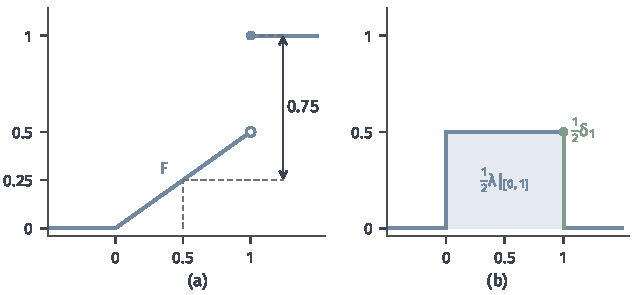
\includegraphics[width=108.000mm]{figures/04-spaces-measures-and-geometry/02-measure/matplotlib/meas-stieltjes-jump/figure.pdf}
  \caption{右连续单调函数$F$确定的Lebesgue--Stieltjes测度。(a)$F$在$[0,1)$上以斜率$1/2$增长，在$x=1$处跳跃$1/2$（实心点为$F(1)=1$，空心点为左极限$1/2$），竖向箭头是$(0.5,1]$的测度$0.75$；(b)$\mu_F$由总量$1/2$、均匀分布在$[0,1]$上的质量（蓝色密度$1/2$）与点质量$\frac12\delta_1$（绿色）组成。}
  \label{fig:meas-stieltjes-jump}
\end{BookInlineFigure}

\paragraph{Lebesgue测度}
取$F(x)=x$，得到$\mathcal B(\mathbb R)$上唯一满足$\lambda((a,b])=b-a$的测度$\lambda$。它没有点质量，所以开、闭、半开区间的测度都等于长度。

延拓定理的证明还给出更多信息。外测度$\lambda^*$由半开区间的可数覆盖定义，而每个半开区间$(a,b]$可以换成略长的开区间$(a,b+\varepsilon2^{-n})$，所以$\lambda^*$也等于用开区间覆盖的总长度的下确界，如图~\ref{fig:meas-outer-cover}所示。

\begin{BookInlineFigure}
  \centering
  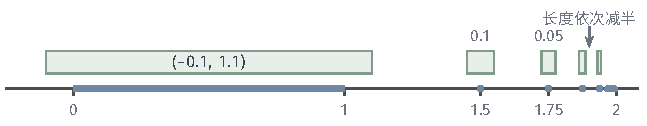
\includegraphics[width=109.552mm]{figures/04-spaces-measures-and-geometry/02-measure/tikz/meas-outer-cover/figure.pdf}
  \caption{用可数个开区间覆盖集合$E=[0,1]\cup\{1.5,1.75,1.875,\dots\}$（蓝色）。绿色区间是一种覆盖：$(-0.1,1.1)$盖住线段部分，长度依次减半的小区间盖住离散的点（只画出前几个）。这个覆盖的总长度为$1.2+0.1\cdot(1+\tfrac12+\tfrac14+\cdots)=1.4$；把各区间进一步缩短，总长度可以任意接近$1$，因此$\lambda^*(E)=1$。}
  \label{fig:meas-outer-cover}
\end{BookInlineFigure}

\begin{definition}[Lebesgue测度]
\label{def:meas-lebesgue}
关于$\lambda^*$为Carathéodory可测的全体集合称为\term{Lebesgue可测集}（Lebesgue measurable set），记作$\mathcal L$；$\lambda^*$在$\mathcal L$上的限制$\lambda$称为实轴上的\term{Lebesgue测度}（Lebesgue measure）。它在$\mathcal B(\mathbb R)$上的限制也称为Borel集上的Lebesgue测度，仍记作$\lambda$。
\end{definition}

覆盖平移后仍是覆盖，长度不变，所以$\lambda^*(E+t)=\lambda^*(E)$对一切$t\in\mathbb R$成立；判据~\eqref{eq:meas-caratheodory-criterion}中的等式随之平移，$\mathcal L$对平移封闭，Lebesgue测度具有平移不变性。

单点被$(x-\varepsilon,x+\varepsilon)$覆盖，测度为$0$，由可数次可加性，可数集的Lebesgue测度为$0$。回到有理点集：$\lambda(\mathbb Q\cap[0,1])=0$，$[0,1]$中无理数集合的测度为$1$。

同时，$[0,1]$是不可数个零测单点之并，整体测度却为$1$。这说明零测集的可数并仍零测，不可数并则不然。

\paragraph{Borel测度与它的完备化}
由Carathéodory定理，$(\mathbb R,\mathcal L,\lambda)$是完备的，且$\mathcal B(\mathbb R)\subseteq\mathcal L$。两者的差别恰好是零测集的子集，下面证明这一点。

设$E\in\mathcal L$且$\lambda(E)<+\infty$。按外测度的定义，对每个$n$有开区间列覆盖$E$且总长小于$\lambda(E)+1/n$，它们的并$U_n$是开集，$\lambda(U_n\setminus E)<1/n$。令$G=\bigcap_nU_n$，它是Borel集，满足
\[
 G\supseteq E,\qquad \lambda(G\setminus E)=0.
\]

对零测集$G\setminus E$再做一次同样的操作，得到Borel零测集$G'\supseteq G\setminus E$。于是
\[
 E=(G\setminus G')\cup(E\cap G'),
\]
第一项是Borel集，第二项包含于Borel零测集。无限测度的$E$切成可数个有限测度的片逐片处理即可。

反过来，$\mathcal L$完备且含$\mathcal B(\mathbb R)$，每个“Borel集并上Borel零测集的子集”都属于$\mathcal L$。所以$(\mathbb R,\mathcal L,\lambda)$正是$(\mathbb R,\mathcal B(\mathbb R),\lambda)$在定理~\ref{thm:meas-completion}意义下的完备化。

对一般的$F$，同样的构造给出$\mu_F$的完备化，它的可测集合族一般随$F$而变：$\mu_F=\delta_0$时，任何不含$0$的集合都是零测集的子集，完备化后全部子集都可测。所以“Borel测度”与“它的完备化”要分开说明，前者的可测范围固定为$\mathcal B(\mathbb R)$，后者的可测范围依赖测度本身。

\paragraph{Cantor集}
零测集是否一定可数？Cantor集给出否定的回答，后面它还会反复出现。

\begin{example}[Cantor集]
\label{ex:meas-cantor-set}
令$C_0=[0,1]$。把$C_{n-1}$中每个闭区间三等分，删去中间的开区间，得到$C_n$，它由$2^n$个长度为$3^{-n}$的闭区间组成，例如$C_1=[0,\tfrac13]\cup[\tfrac23,1]$。令
\[
 C=\bigcap_{n\geq0}C_n,
\]
称为\term{Cantor集}（Cantor set）。它是闭集的交，因而是闭集，也是Borel集。由$C\subseteq C_n$，
\[
 \lambda(C)\leq\lambda(C_n)=2^n\cdot3^{-n}=(2/3)^n\to0,
\]
所以$\lambda(C)=0$。

也可以从被删去的部分验算：第$n$步删去$2^{n-1}$个长度为$3^{-n}$的区间，总长度为
\[
 \sum_{n\geq1}\frac{2^{n-1}}{3^n}=\frac{1/3}{1-2/3}=1.
\]
被删去的总长度已经是$1$，留给$C$的长度只能是$0$。
\end{example}

图~\ref{fig:meas-cantor-set}画出了前四步。每一行的总长度按比例$2/3$缩小，同时区间的个数翻倍；留下的点集越来越稀，却始终非空。

\begin{BookInlineFigure}
  \centering
  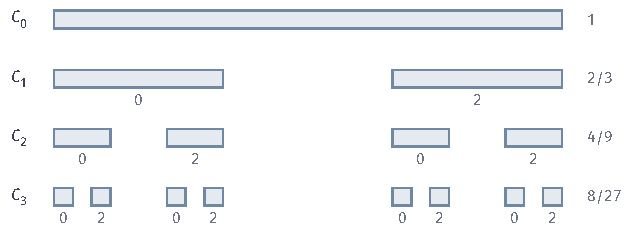
\includegraphics[width=107.142mm]{figures/04-spaces-measures-and-geometry/02-measure/tikz/meas-cantor-set/figure.pdf}
  \caption{Cantor集构造的前四步。第$n$行$C_n$由$2^n$个长度为$3^{-n}$的闭区间组成，右侧数字是总长度$(2/3)^n$；区间下方的三进制数字$0$或$2$记录这一步选择左段还是右段。}
  \label{fig:meas-cantor-set}
\end{BookInlineFigure}

Cantor集测度为零，却不可数。对每个$0$--$1$序列$s=(s_1,s_2,\dots)$，令
\[
 \phi(s)=\sum_{k\geq1}\frac{2s_k}{3^k},
\]
即三进制展开中只用数字$0$与$2$的数。前$n$位数字决定了前$n$步每一步选左段（数字$0$）还是右段（数字$2$），所以$\phi(s)\in C_n$对每个$n$成立，从而$\phi(s)\in C$。

$\phi$是单射。设$s\neq t$，第一个不同的位置为$k$，不妨$s_k=1$、$t_k=0$，则后面各项最多抵消$\sum_{j>k}2\cdot3^{-j}=3^{-k}$，于是
\[
 \phi(s)-\phi(t)\geq2\cdot3^{-k}-3^{-k}=3^{-k}>0.
\]
全体$0$--$1$序列不可数，故$C$不可数。零测性度量集合占据的长度，基数度量元素的多少，二者不能互相推出。

Cantor集还说明完备化确实增加了集合。$\lambda(C)=0$，由完备性，$C$的全部子集都Lebesgue可测，$C$与$\mathbb R$等势，所以这些子集和$\mathbb R$的全部子集一样多；而Borel集的个数只有连续统那么多，严格少于$\mathbb R$的子集个数。Borel集个数的证明要用到超限归纳，篇幅较长，读者可查阅\scite{math-folland1999real}。结论是：存在不是Borel集的Lebesgue可测集。

反过来，也存在不Lebesgue可测的集合。在$[0,1)$上规定$x\sim y$当且仅当$x-y\in\mathbb Q$，用选择公理从每个等价类选一个代表，组成集合$V$。令$\{r_k\}$为$[0,1)$中全体有理数，$V_k$为$V$按模$1$平移$r_k$的结果。这些$V_k$两两不交，并为$[0,1)$。

若$V$可测，平移不变性给出$\lambda(V_k)=\lambda(V)$，于是
\[
 1=\lambda([0,1))=\sum_k\lambda(V_k)=\sum_k\lambda(V).
\]
右边要么是$0$，要么是$+\infty$，不可能等于$1$。所以测度只能定义在某个$\sigma$代数上，不能假定全部子集都可测。

\paragraph{多维Lebesgue测度}
在$\mathbb R^d$上，把区间换成左开右闭矩形$\prod_{i=1}^d(a_i,b_i]$，长度换成体积。它们的有限不交并组成集合代数，体积在其上的可数可加性与一维相同：闭矩形是紧集，可数覆盖化为有限覆盖后，用全部矩形的边坐标把大矩形切成网格，逐块比较体积，就得到引理~\ref{lem:meas-finite-cover}的$d$维版本。

由延拓定理，得到$\mathcal B(\mathbb R^d)$上唯一满足$\lambda_d(R)=\lvert R\rvert$的测度$\lambda_d$，称为$d$维Lebesgue测度。它同样平移不变，其完备化的可测集称为$d$维Lebesgue可测集。$\lambda_d$与$d$个一维Lebesgue测度的乘积相同，这需要第~\ref{chap:integration}章的乘积测度来说明。

\section{有符号测度}
\label{sec:meas-signed}

测度只取非负值。可是很多量天然有正有负：一根杆上同时分布着正电荷与负电荷，一笔账在不同科目上有收入也有支出，两个概率分布在各个集合上的差有时为正、有时为负。最直接的模型是两个测度之差$\eta(A)=\nu(A)-\mu(A)$。本节研究这类赋值：它在哪里取正、在哪里取负，能否唯一地写回两个测度之差，以及怎样度量正负两方面的总量。积分尚未定义，本节只在集合层面讨论。

\subsection{正集与负集}
\label{sec:meas-positive-negative-sets}

\paragraph{从测度之差到有符号测度}
设$\nu,\mu$是$(X,\mathcal A)$上的测度，$\mu$有限。对两两不交的可测集$A_1,A_2,\dots$，两个测度各自可数可加，并且$\sum_n\mu(A_n)$收敛到有限值，所以
\[
 \eta\Bigl(\bigcup_nA_n\Bigr)=\sum_n\nu(A_n)-\sum_n\mu(A_n)=\sum_n\bigl(\nu(A_n)-\mu(A_n)\bigr)=\sum_n\eta(A_n).
\]
中间一步把两个级数逐项相减，这在至少一个级数有限时成立。可见$\eta=\nu-\mu$保留了可数可加性，只是不再非负；它可以取$+\infty$，但不会取$-\infty$。

两个无限测度不能直接相减。在$\mathbb N$上取计数测度$\nu$与$\mu=2\nu$，对无限集$A$，$\nu(A)-\mu(A)=+\infty-(+\infty)$没有定义。即使把它理解为某个数，也会和可数可加性冲突：$\mathbb N$分成单点后每块的差都是$-1$，级数和为$-\infty$；分成偶数集与奇数集后两块的差都没有定义。所以有符号测度必须禁止同时出现两种无穷。

\begin{definition}[有符号测度]
\label{def:meas-signed}
可测空间$(X,\mathcal A)$上的\term{有符号测度}（signed measure）是映射$\eta:\mathcal A\to[-\infty,+\infty]$，满足：$\eta$至多取$+\infty$与$-\infty$中的一个；$\eta(\varnothing)=0$；对任意两两不交的$A_1,A_2,\dots\in\mathcal A$，
\[
 \eta\Bigl(\bigcup_{n\geq1}A_n\Bigr)=\sum_{n\geq1}\eta(A_n),
\]
其中左端有限时，右端级数绝对收敛。若$\eta$只取有限实数值，称为\term{有限有符号测度}（finite signed measure）。
\end{definition}

“至多取一种无穷”保证了右端级数总有意义：各项中不会同时出现$+\infty$与$-\infty$。要求左端有限时级数绝对收敛，是因为不交集合的并与排列次序无关，右端也必须与次序无关；按实数级数的重排定理，这等价于绝对收敛。测度是有符号测度的特例，任意有限测度之差是有限有符号测度。

有符号测度是给\emph{集合}赋予实数的规则，不要与某些\emph{点}上取负值的函数混淆。$\eta(A)<0$表示集合$A$上的负质量多于正质量，这个数由整个集合决定。

\begin{example}[正负抵消]
\label{ex:meas-signed-weights}
取$X=\{1,2,3,4\}$及全部子集，规定单点值$\eta(\{1\})=2$，$\eta(\{2\})=-1$，$\eta(\{3\})=1$，$\eta(\{4\})=-2$，并令$\eta(A)=\sum_{i\in A}\eta(\{i\})$。它是有限有符号测度，也可以写成$\nu-\mu$，其中$\nu=2\delta_1+\delta_3$，$\mu=\delta_2+2\delta_4$。

计算几个值：$\eta(X)=2-1+1-2=0$，$\eta(\{1,2\})=1$，$\eta(\{1,3\})=3$，$\eta(\{2,4\})=-3$。全空间上的值为零只是正负抵消的结果；在$\{1,3\}$与$\{2,4\}$上，$\eta$的绝对值都达到$3$。所以$\eta(X)$很小甚至为零，不能说明$\eta$在各处都小。
\end{example}

例中的$\eta$还可以写成$(\nu+\delta_1)-(\mu+\delta_1)$。同一个有符号测度有许多种“测度减测度”的表示。我们要找的是由$\eta$本身确定、没有多余抵消的一种，第一步是找出$\eta$在哪里取正、在哪里取负。

\paragraph{正集与负集的定义}
只看$\eta(P)\geq0$并不够：例~\ref{ex:meas-signed-weights}中$\eta(\{1,2\})=1\geq0$，它的子集$\{2\}$却取$-1$。$\{1,2\}$整体为正，内部仍藏着负质量。要作为“正区域”，集合的每个可测部分都必须非负。

\begin{definition}[正集与负集]
\label{def:meas-positive-set}
设$\eta$是$(X,\mathcal A)$上的有符号测度。若$P\in\mathcal A$的每个可测子集$E$都满足$\eta(E)\geq0$，称$P$为$\eta$的\term{正集}（positive set）；若$N\in\mathcal A$的每个可测子集$E$都满足$\eta(E)\leq0$，称$N$为$\eta$的\term{负集}（negative set）。
\end{definition}

在例~\ref{ex:meas-signed-weights}中，$\{1,3\}$是正集，$\{2,4\}$是负集，$\{1,2\}$两者都不是。正集与负集可以同时是二者：$\eta$在其每个可测子集上都取零的集合，既是正集又是负集。

正集的可测子集仍是正集，可数个正集的并也是正集。若$P_1,P_2,\dots$是正集，$E\subseteq\bigcup_nP_n$可测，令$E_1=E\cap P_1$，$E_n=(E\cap P_n)\setminus(P_1\cup\dots\cup P_{n-1})$，则$E_n$是$P_n$的可测子集且两两不交，$\eta(E)=\sum_n\eta(E_n)\geq0$。负集同理。这两条封闭性是下面把正负区域拼起来的依据。

\subsection{Hahn分解与Jordan分解}
\label{sec:meas-hahn-jordan}

例~\ref{ex:meas-signed-weights}中，只要把$X$分成$\{1,3\}$与$\{2,4\}$，$\eta$在前一部分的每个子集上非负，在后一部分的每个子集上非正。一般的有符号测度是否也能一刀切成正、负两个区域？先对有限有符号测度证明，再说明扩展值的情形。

\paragraph{两条准备性质}
构造正负区域的思路是寻找使$\eta$最小的可测集。为此先要知道$\eta$的取值不会无限地向下延伸，并且单调集合列的连续性在有符号情形仍然成立。

\begin{lemma}[有限有符号测度有界]
\label{lem:meas-signed-bounded}
有限有符号测度$\eta$有界：存在$M<\infty$，使$\lvert\eta(A)\rvert\leq M$对一切$A\in\mathcal A$成立。
\end{lemma}

\begin{proof}
称可测集$A$是\emph{无界的}，如果$\sup\{\lvert\eta(E)\rvert:E\subseteq A,\ E\in\mathcal A\}=\infty$。设$X$是无界的，我们构造两两不交的可测集$B_1,B_2,\dots$，使每个$\lvert\eta(B_n)\rvert\geq1$。

设$A$无界。取可测子集$E\subseteq A$使$\lvert\eta(E)\rvert\geq\lvert\eta(A)\rvert+1$，则$\lvert\eta(A\setminus E)\rvert\geq\lvert\eta(E)\rvert-\lvert\eta(A)\rvert\geq1$。$E$与$A\setminus E$中至少有一个无界：否则$A$的任一可测子集$F$满足$\lvert\eta(F)\rvert\leq\lvert\eta(F\cap E)\rvert+\lvert\eta(F\setminus E)\rvert$，右边两项都有界。把无界的一块记为$A'$，另一块记为$B$，则$B\subseteq A\setminus A'$且$\lvert\eta(B)\rvert\geq1$。

从$A_0=X$出发反复执行这一步，得到无界集$A_0\supseteq A_1\supseteq\cdots$及$B_n\subseteq A_{n-1}\setminus A_n$，这些$B_n$两两不交。按定义~\ref{def:meas-signed}，$\sum_n\eta(B_n)$收敛到有限值$\eta(\bigcup_nB_n)$，通项必须趋于零，与$\lvert\eta(B_n)\rvert\geq1$矛盾。
\end{proof}

\begin{lemma}[有符号测度的单调连续性]
\label{lem:meas-signed-continuity}
设$\eta$是有限有符号测度。若$A_1\subseteq A_2\subseteq\cdots$，则$\eta(\bigcup_nA_n)=\lim_n\eta(A_n)$；若$A_1\supseteq A_2\supseteq\cdots$，则$\eta(\bigcap_nA_n)=\lim_n\eta(A_n)$。
\end{lemma}

\begin{proof}
对递增集合列，令$D_1=A_1$，$D_n=A_n\setminus A_{n-1}$，它们两两不交，$\bigcup_nA_n=\bigcup_nD_n$，部分和$\sum_{k\leq n}\eta(D_k)=\eta(A_n)$，由可数可加性得结论。对递减集合列，$A_1\setminus A_n$递增，并为$A_1\setminus\bigcap_nA_n$；由已证部分及$\eta(A_1\setminus B)=\eta(A_1)-\eta(B)$（各项有限），得$\eta(A_1)-\eta(\bigcap_nA_n)=\lim_n(\eta(A_1)-\eta(A_n))$。
\end{proof}

与测度不同，这里递减情形不需要另加有限性假设，因为$\eta$本身只取有限值。

\paragraph{Hahn分解}
若某个可测集$D$使$\eta$达到最小值，那么从$D$中拿走一个正值子集，或向$D$中添入一个负值的外部集合，都会让取值更小，这不可能；于是$D$是负集，补集是正集。难点在于证明最小值确实能被某个集合达到。

\begin{theorem}[Hahn分解]
\label{thm:meas-hahn}
设$\eta$是$(X,\mathcal A)$上的有符号测度。则存在$P\in\mathcal A$，使$P$是$\eta$的正集，$N=X\setminus P$是$\eta$的负集。这样的一对$(P,N)$称为$\eta$的\term{Hahn分解}（Hahn decomposition）。若$(P',N')$是另一组Hahn分解，则$P\cap N'$与$P'\cap N$的每个可测子集上$\eta$都取零。
\end{theorem}

\begin{proof}
先设$\eta$有限。令$m=\inf_{A\in\mathcal A}\eta(A)$。由引理~\ref{lem:meas-signed-bounded}，$m$是有限实数，又$\eta(\varnothing)=0$，故$m\leq0$。对每个$n$取可测集$A_n$使$\eta(A_n)<m+2^{-n}$。

第一步说明两个近乎最小的集合取交后仍近乎最小。对可测集$A,B$，有限可加性给出$\eta(A\cup B)+\eta(A\cap B)=\eta(A)+\eta(B)$；又$\eta(A\cup B)\geq m$，所以$\eta(A\cap B)\leq\eta(A)+\eta(B)-m$。固定$n$，对$k\geq n$令$C_{n,k}=A_n\cap\dots\cap A_k$，对$k$归纳得
\[
 \eta(C_{n,k+1})\leq\eta(C_{n,k})+\eta(A_{k+1})-m<m+\sum_{j=n}^{k+1}2^{-j}<m+2^{1-n}.
\]

第二步取极限。$C_{n,k}$关于$k$递减，令$C_n=\bigcap_{k\geq n}A_k$；由引理~\ref{lem:meas-signed-continuity}，$\eta(C_n)\leq m+2^{1-n}$。$C_n$关于$n$递增，令$D=\bigcup_nC_n$；再由该引理，$\eta(D)=\lim_n\eta(C_n)\leq m$。另一方面$\eta(D)\geq m$，所以$\eta(D)=m$，最小值被$D$达到。

第三步验证符号。若可测集$E\subseteq D$满足$\eta(E)>0$，则$\eta(D\setminus E)=m-\eta(E)<m$，矛盾，所以$D$是负集。若可测集$E\subseteq X\setminus D$满足$\eta(E)<0$，则$\eta(D\cup E)=m+\eta(E)<m$，同样矛盾，所以$X\setminus D$是正集。取$N=D$，$P=X\setminus D$即可。

对允许取一种无穷值的$\eta$，存在性的证明需要另一条引理：有限正值的集合中总能找到正值的正集。由此可以在正集中取使$\eta$接近上确界的一列，再用正集的可数并封闭性拼成最大的正区域。这里不给出这部分证明，可参考Folland的《Real Analysis》第3章。

最后看两组分解的差别，这一步对两种情形都适用。$P\cap N'$既是正集$P$的子集，又是负集$N'$的子集，它的每个可测子集$E$同时满足$\eta(E)\geq0$与$\eta(E)\leq0$，即$\eta(E)=0$。$P'\cap N$同理。
\end{proof}

Hahn分解一般不唯一：$\eta$在其上完全为零的区域可以划给任意一侧。在实轴上令$\eta=\lambda|_{[0,1]}-\lambda|_{[2,3]}$，$P_1=(-\infty,3/2)$与$P_2=(-\infty,2)$都给出Hahn分解，两者相差的$[3/2,2)$上$\eta$的每个子集都取零，见图~\ref{fig:meas-hahn-decomposition}。正区域还可以只差一个Lebesgue零测集，例如把点$1/2$从$P_1$移到负区域一侧。

\begin{figure}[!htbp]
  \centering
  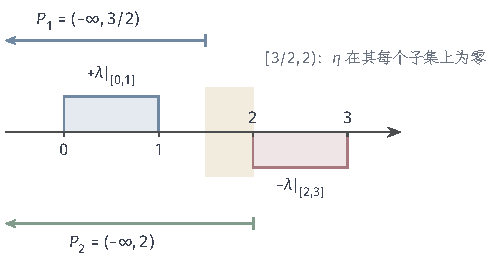
\includegraphics[width=84.06mm]{figures/02-abstract-mathematics/01-metric-and-measure/tikz/c2-hahn-decomposition/figure.pdf}
  \caption{Hahn分解的区域选择不唯一。$\eta=\lambda|_{[0,1]}-\lambda|_{[2,3]}$，蓝块在$[0,1]$上表示正的长度，红块在$[2,3]$上表示负的长度，块高表示长度测度前的系数$\pm1$。正区域可以取$P_1=(-\infty,3/2)$，也可以取$P_2=(-\infty,2)$；二者之差$[3/2,2)$（黄色）的每个可测子集上$\eta$都为零，所以放在哪一侧都不改变符号要求。}
  \label{fig:meas-hahn-decomposition}
\end{figure}

\paragraph{Jordan分解}
区域可以不同，限制在区域上的质量却是唯一的。把$\eta$分别限制到正区域与负区域，就得到两个测度。

\begin{theorem}[Jordan分解]
\label{thm:meas-jordan}
设$\eta$是有符号测度，$(P,N)$是它的一组Hahn分解。令
\[
 \eta^+(A)=\eta(A\cap P),\qquad \eta^-(A)=-\eta(A\cap N),\qquad A\in\mathcal A .
\]
则$\eta^+,\eta^-$是测度，其中至少一个有限，$\eta=\eta^+-\eta^-$，且$\eta^+(N)=\eta^-(P)=0$；它们不依赖于Hahn分解的选取。反过来，若$\eta=\alpha-\beta$，其中$\alpha,\beta$是测度、至少一个有限，并且存在可测集$S$使$\beta(S)=0$、$\alpha(X\setminus S)=0$，则$\alpha=\eta^+$，$\beta=\eta^-$。这个表示称为$\eta$的\term{Jordan分解}（Jordan decomposition），$\eta^+$、$\eta^-$分别称为$\eta$的\term{正变差}（positive variation）与\term{负变差}（negative variation）。
\end{theorem}

\begin{proof}
$A\cap P$是正集的子集，所以$\eta^+(A)\geq0$；同理$\eta^-(A)\geq0$。可数可加性直接来自$\eta$：若$A_n$两两不交，则$A_n\cap P$也两两不交。若$\eta$不取$+\infty$，则$\eta^+(X)=\eta(P)<+\infty$；若不取$-\infty$，则$\eta^-$有限。由$A=(A\cap P)\cup(A\cap N)$得$\eta(A)=\eta^+(A)-\eta^-(A)$，右边至多一项无穷，所以差有意义。$\eta^+(N)=\eta(\varnothing)=0$，$\eta^-(P)=0$。

再看与Hahn分解无关。设$(P',N')$是另一组分解。由定理~\ref{thm:meas-hahn}，$A\cap P\cap N'$与$A\cap P'\cap N$上$\eta$取零，因此
\[
 \eta(A\cap P)=\eta(A\cap P\cap P')+\eta(A\cap P\cap N')=\eta(A\cap P\cap P')=\eta(A\cap P'),
\]
最后一步对$P'$作同样的拆分。$\eta^-$同理。

最后证唯一性。设$\eta=\alpha-\beta$与$S$如定理所述。对$S$的可测子集$E$，$\eta(E)=\alpha(E)-0\geq0$；对$X\setminus S$的可测子集$E$，$\eta(E)=0-\beta(E)\leq0$。所以$(S,X\setminus S)$本身是一组Hahn分解。由已证的无关性，$\eta^+(A)=\eta(A\cap S)=\alpha(A\cap S)=\alpha(A)$，最后一步用了$\alpha(A\setminus S)=0$。同理$\beta=\eta^-$。
\end{proof}

定理中“存在$S$使$\beta(S)=0$、$\alpha(X\setminus S)=0$”说的是两个测度分别集中在两个不交的集合上，这种关系称为相互奇异，第~\ref{chap:measure-densities}章再系统比较。唯一性离不开这一条件。仍取$\eta=\lambda|_{[0,1]}-\lambda|_{[2,3]}$，它的Jordan分解是$\eta^+=\lambda|_{[0,1]}$、$\eta^-=\lambda|_{[2,3]}$。另一方面，令$\alpha=\lambda|_{[0,3]}$，$\beta=\lambda|_{[1,2]}+2\lambda|_{[2,3]}$，逐段检查系数：$[0,1]$上为$1-0$，$[1,2]$上为$1-1$，$[2,3]$上为$1-2$，所以同样有$\alpha-\beta=\eta$。但$\alpha,\beta$在$[1,3]$上重叠，总量都是$3$，而$\eta^\pm$的总量都是$1$。

这种多余的重叠只增不减。对任意表示$\eta=\alpha-\beta$（$\alpha,\beta$为测度，至少一个有限）及任意$A\in\mathcal A$，
\[
 \eta^+(A)=\eta(A\cap P)=\alpha(A\cap P)-\beta(A\cap P)\leq\alpha(A\cap P)\leq\alpha(A),
\]
同理$\eta^-(A)\leq\beta(A)$。所以Jordan分解是所有“测度减测度”表示中最小的一个。两种分解的输出不同：Hahn分解输出一个集合划分，它不唯一；Jordan分解输出两个测度，它唯一。

\subsection{全变差}
\label{sec:meas-total-variation}

$\lvert\eta(A)\rvert$衡量的是集合$A$上正负相抵后的净值，例~\ref{ex:meas-signed-weights}说明它可能掩盖很大的局部差别。要累计正负两方面的全部质量，应当把正变差与负变差相加，而不是相减。

\begin{definition}[全变差]
\label{def:meas-total-variation}
设$\eta$是有符号测度，$\eta=\eta^+-\eta^-$是它的Jordan分解。称测度
\[
 \lvert\eta\rvert=\eta^++\eta^-
\]
为$\eta$的\term{全变差测度}（total variation measure），称$\lvert\eta\rvert(X)$为$\eta$的\term{全变差}（total variation）。
\end{definition}

\paragraph{分割刻画}
$\lvert\eta\rvert$也可以不借助Jordan分解，直接从$\eta$的取值读出：把$A$切成有限块，对每块的净值取绝对值再相加。切得越合适，抵消越少；最合适的切法就是沿Hahn分解切开。

\begin{theorem}[全变差的分割刻画]
\label{thm:meas-total-variation-partition}
对每个$A\in\mathcal A$，
\[
 \lvert\eta\rvert(A)=\sup\Bigl\{\sum_{i=1}^k\lvert\eta(A_i)\rvert:\ k\geq1,\ A_1,\dots,A_k\in\mathcal A\text{两两不交},\ \bigcup_{i=1}^kA_i=A\Bigr\}.
\]
\end{theorem}

\begin{proof}
对$A$的任一有限可测分割，
\[
 \sum_i\lvert\eta(A_i)\rvert=\sum_i\lvert\eta^+(A_i)-\eta^-(A_i)\rvert\leq\sum_i\bigl(\eta^+(A_i)+\eta^-(A_i)\bigr)=\lvert\eta\rvert(A),
\]
所以上确界不超过$\lvert\eta\rvert(A)$。取Hahn分解$(P,N)$及分割$A_1=A\cap P$、$A_2=A\cap N$，则$\lvert\eta(A_1)\rvert+\lvert\eta(A_2)\rvert=\eta^+(A)+\eta^-(A)=\lvert\eta\rvert(A)$，上确界被达到。
\end{proof}

回到例~\ref{ex:meas-signed-weights}。不分割时$\lvert\eta(X)\rvert=0$；分成$\{1,2\}$与$\{3,4\}$时得$\lvert1\rvert+\lvert-1\rvert=2$；分成$\{1,3\}$与$\{2,4\}$时得$3+3=6$。再细分也不会超过$6$，因为四个单点上的绝对值之和为$2+1+1+2=6$。所以$\lvert\eta\rvert(X)=6$，正好由正负区域的分割取得，见图~\ref{fig:meas-total-variation-partition}。

\begin{figure}[!htbp]
  \centering
  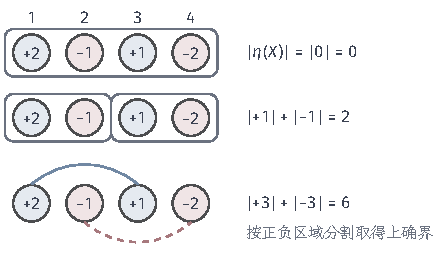
\includegraphics[width=75.128mm]{figures/02-abstract-mathematics/01-metric-and-measure/tikz/c2-total-variation-partition/figure.pdf}
  \caption{用分割读取全变差。四个点的权重为$+2,-1,+1,-2$。第一行不分割，净值为$0$；第二行把相邻的正负点合在一起，仍有抵消，绝对值之和为$2$；第三行按符号分组（蓝色实弧连接正点，红色虚弧连接负点），没有抵消，绝对值之和为$6=\lvert\eta\rvert(X)$。}
  \label{fig:meas-total-variation-partition}
\end{figure}

\paragraph{净值与总量}
由分割刻画取平凡分割$\{A\}$，立即得到$\lvert\eta(A)\rvert\leq\lvert\eta\rvert(A)$：左边允许抵消，右边累计正负变化的总量。特别地，$\lvert\eta\rvert(A)=0$当且仅当$\eta$在$A$的每个可测子集上都取零。所以$\lvert\eta\rvert$的零测集正是$\eta$完全看不见的集合；对有符号测度说“几乎处处”时，都相对于$\lvert\eta\rvert$来理解。

\paragraph{有限与扩展值两种情形}
若$\eta$是有限有符号测度，$\eta^+$与$\eta^-$都有限，$\lvert\eta\rvert$是有限测度，并且$\lvert\eta(A)\rvert\leq\lvert\eta\rvert(X)<\infty$对一切$A$成立，这与引理~\ref{lem:meas-signed-bounded}一致。若$\eta$取$+\infty$，则$\eta^+$无限而$\eta^-$有限，$\lvert\eta\rvert$在某些集合上为$+\infty$，此时只能在$\lvert\eta\rvert$有限的集合上作数值比较。

两个概率测度$P,Q$之差$\eta=P-Q$属于前一种情形。由$\eta(X)=0$得$\eta^+(X)=\eta^-(X)=\tfrac12\lvert\eta\rvert(X)$。又对每个可测集$A$有$\eta(A)\leq\eta^+(A)\leq\eta^+(X)$，取$A=P$时等号成立，所以
\[
 \tfrac12\lvert P-Q\rvert(X)=\eta^+(X)=\sup_{A\in\mathcal A}\bigl(P(A)-Q(A)\bigr).
\]
后续估计积分误差时，常用总量有限的$\lvert\eta\rvert$控制正负两方面的贡献；一个有符号测度何时能写成某个可积函数乘以参考测度，留到第~\ref{chap:measure-densities}章，那里同样要区分总量有限与允许扩展值的情形。

\section{可测映射}
\label{sec:meas-measurable-maps}

有了测度，下一步是把它用到函数上：一根细杆各处的线密度不同，总质量是多少；一个随机实验的结果被读成一个数，这个数落在某个区间里的概率是多少。每当对函数的输出提出“是否落在某集合中”的问题，就需要在输入端测量相应的点集。本节用原像刻画这一要求，先给出可测映射的定义与判据，再证明数值函数的常见运算和可数极限保持可测性，最后用只取有限个值的简单函数从下方逼近非负可测函数，为下一章定义积分准备对象。

\subsection{可测映射}
\label{sec:meas-measurable-map-def}

\paragraph{原像与可测性}
对映射$f:X\to Y$与$B\subseteq Y$，原像$f^{-1}(B)=\{x\in X:f(x)\in B\}$是“输出落在$B$中”的那些输入。原像对任意映射都有意义，并不要求$f$可逆。若输出端能提出的每个集合问题，在输入端都对应一个可测集合，就说$f$可测。

\begin{definition}[可测映射]
\label{def:meas-measurable-map}
设$(X,\mathcal A)$、$(Y,\mathcal B)$是可测空间。若对每个$B\in\mathcal B$都有$f^{-1}(B)\in\mathcal A$，称映射$f:X\to Y$为$\mathcal A/\mathcal B$-\term{可测映射}（measurable map），简称可测。
\end{definition}

可测性同时取决于两端的$\sigma$代数。在$X=\{1,2,3,4\}$上取由$\varnothing,\{1,2\},\{3,4\},X$组成的$\sigma$代数$\mathcal A$，在$Y=\{a,b\}$上取$\mathcal P(Y)$。令$f(1)=f(2)=a$、$f(3)=f(4)=b$，则$f^{-1}(\{a\})=\{1,2\}$、$f^{-1}(\{b\})=\{3,4\}$都可测，$f$可测。令$g(1)=a$、$g(2)=g(3)=g(4)=b$，则$g^{-1}(\{a\})=\{1\}\notin\mathcal A$，$g$不可测：输入端只知道点属于哪一组，无法回答“输出是否为$a$”。若把$Y$上的$\sigma$代数换成$\{\varnothing,Y\}$，$g$又变成可测的，因为输出端不再提出任何非平凡问题。

这与连续性的定义形式相同，内容不同。第~\ref{chap:topological-spaces}章的连续映射要求开集的原像是开集，可测映射要求可测集的原像是可测集。连续性关心邻近关系是否保持，可测性只关心集合问题能否在输入端回答，与距离和开集没有直接关系。

\paragraph{生成族判据}
直接检查$\mathcal B$中的每个集合往往做不到，例如$\mathcal B(\mathbb R)$中的集合无法逐一列出。原像与集合运算可交换，所以只需检查生成族。

\begin{lemma}[生成族判据]
\label{lem:meas-generator-criterion}
设$\mathcal B=\sigma(\mathcal C)$。若对每个$C\in\mathcal C$都有$f^{-1}(C)\in\mathcal A$，则$f$是$\mathcal A/\mathcal B$可测的。
\end{lemma}

\begin{proof}
令$\mathcal E=\{B\subseteq Y:f^{-1}(B)\in\mathcal A\}$。由$f^{-1}(Y)=X$、$f^{-1}(Y\setminus B)=X\setminus f^{-1}(B)$与$f^{-1}(\bigcup_nB_n)=\bigcup_nf^{-1}(B_n)$，$\mathcal E$是$Y$上的$\sigma$代数。它含$\mathcal C$，所以含$\sigma(\mathcal C)=\mathcal B$。
\end{proof}

由定义还可以直接得到复合规则。若$f:(X,\mathcal A)\to(Y,\mathcal B)$与$g:(Y,\mathcal B)\to(Z,\mathcal C)$都可测，则对$C\in\mathcal C$，$(g\circ f)^{-1}(C)=f^{-1}(g^{-1}(C))\in\mathcal A$，所以$g\circ f$可测。这里要求中间空间$Y$上两次使用的是同一个$\sigma$代数$\mathcal B$。

\paragraph{可测函数}
最常用的可测映射取实数值。目标端取$\mathcal B(\mathbb R)$；允许取$\pm\infty$时，在扩展实数$[-\infty,+\infty]$上取由$\mathcal B(\mathbb R)$与两个单点$\{-\infty\},\{+\infty\}$生成的$\sigma$代数。由定理~\ref{thm:meas-borel-generators}，半直线$(a,+\infty)$生成$\mathcal B(\mathbb R)$，再加上$\{+\infty\}=\bigcap_n(n,+\infty]$与$\{-\infty\}=[-\infty,+\infty]\setminus\bigcup_n(-n,+\infty]$，可知$(a,+\infty]$生成扩展实数上的这个$\sigma$代数。判据于是化为检查阈值集合。

\begin{definition}[可测函数]
\label{def:meas-measurable-function}
设$(X,\mathcal A)$是可测空间。若$f:X\to[-\infty,+\infty]$对每个$a\in\mathbb R$都有$\{f>a\}=\{x:f(x)>a\}\in\mathcal A$，称$f$为\term{可测函数}（measurable function）。当$(X,\mathcal A)=(\mathbb R^d,\mathcal B(\mathbb R^d))$时，称为\term{Borel可测函数}（Borel measurable function）。
\end{definition}

由生成族判据，实值函数$f$可测等价于它是$\mathcal A/\mathcal B(\mathbb R)$可测映射；只检查有理数$a$也够用。用补集与可数运算还可得到其他阈值集合，例如$\{f\geq a\}=\bigcap_n\{f>a-1/n\}$、$\{f\leq a\}=X\setminus\{f>a\}$，它们都可测。复值函数$f=u+\mathrm iv$称为可测，是指实部$u$与虚部$v$都可测。

集合的可测性与函数的可测性通过指示函数相连。对$A\subseteq X$，$\{\mathbf 1_A>a\}$在$a<0$时为$X$，在$0\leq a<1$时为$A$，在$a\geq1$时为$\varnothing$，所以$\mathbf 1_A$可测当且仅当$A\in\mathcal A$。例如$\mathbf 1_{\mathbb Q}$在$(\mathbb R,\mathcal B(\mathbb R))$上可测，因为$\mathbb Q$是Borel集；第~\ref{sec:meas-jordan}小节中它对应的集合连Jordan可测都不是。

\paragraph{连续映射与可测性}
设$X,Y$是度量空间，$f:X\to Y$连续。开集的原像是开集，因而属于$\mathcal B(X)$；开集生成$\mathcal B(Y)$，由生成族判据，$f$是$\mathcal B(X)/\mathcal B(Y)$可测的。所以连续函数都是Borel可测函数。

逆向结论不成立。阶跃函数$H=\mathbf 1_{[0,+\infty)}$的阈值集合是$\mathbb R$、$[0,+\infty)$或$\varnothing$，都是Borel集，所以$H$是Borel可测函数，但它在$0$处不连续；$\mathbf 1_{\mathbb Q}$处处不连续，却同样Borel可测。可测性只问阈值集合是否在允许测量的集合族里，对函数的局部变化没有任何要求。

上面的结论依赖两端都取Borel结构。若把两端都换成Lebesgue可测集$\mathcal L$，连续函数$f:\mathbb R\to\mathbb R$未必$\mathcal L/\mathcal L$可测：可以构造连续严格单调的$f$与零测集的子集$S$（由完备性，$S\in\mathcal L$），使$f^{-1}(S)$不Lebesgue可测。这里不展开构造，只记住：可测性必须写清两端的集合族，不能把目标端的Borel结构随意换成某个测度的完备化。本书中实值函数的目标端总取Borel结构。

\subsection{可测函数的运算}
\label{sec:meas-function-operations}

\paragraph{代数运算}
可测函数经过加、乘、取绝对值等运算后仍然可测。困难在于和的阈值集合$\{f+g>a\}$不能直接写成$f$与$g$各自阈值集合的有限组合，需要用有理数作可数分拆。

\begin{theorem}[可测函数的运算]
\label{thm:meas-function-operations}
设$f,g:X\to\mathbb R$可测，$c\in\mathbb R$，$\varphi:\mathbb R\to\mathbb R$连续。则$cf$、$f+g$、$\varphi\circ f$、$fg$、$\lvert f\rvert$、$\max\{f,g\}$、$\min\{f,g\}$都可测；若$g$处处不为零，$f/g$也可测。
\end{theorem}

\begin{proof}
$\varphi\circ f$是可测映射与Borel可测的连续函数之复合，所以可测。取$\varphi(t)=ct$、$\lvert t\rvert$、$t^2$，得$cf$、$\lvert f\rvert$、$f^2$可测。

对和，若$f(x)+g(x)>a$，则$f(x)>a-g(x)$，在两者之间取有理数$q$，有$f(x)>q$且$g(x)>a-q$；反之这两式蕴含$f(x)+g(x)>a$。所以
\[
 \{f+g>a\}=\bigcup_{q\in\mathbb Q}\bigl(\{f>q\}\cap\{g>a-q\}\bigr),
\]
是可数个可测集合之并。于是$f-g=f+(-1)g$可测。积由$fg=\tfrac14\bigl((f+g)^2-(f-g)^2\bigr)$得到，最大值与最小值由$\max\{f,g\}=\tfrac12(f+g+\lvert f-g\rvert)$与$\min\{f,g\}=\tfrac12(f+g-\lvert f-g\rvert)$得到。若$g$处处非零，$t\mapsto1/t$在$\mathbb R\setminus\{0\}$上连续，把它在$0$处任意赋值得到的Borel函数与$g$复合，可知$1/g$可测，从而$f/g$可测。
\end{proof}

复值可测函数按实部与虚部计算，同样对加法、乘法和取模封闭：$\lvert f\rvert=\sqrt{u^2+v^2}$是连续函数作用于$(u,v)$，可以先由$u^2+v^2$可测再取平方根。

\paragraph{扩展实值的运算范围}
允许取扩展实数值时，运算本身可能没有定义。$f+g$在$f(x)=+\infty$、$g(x)=-\infty$的点没有意义，必须先说明这样的点不出现，或者在那里另作约定；乘积还要约定$0\cdot(\pm\infty)$，本书取$0\cdot(\pm\infty)=0$。只有在这些点上的值确定以后，才能谈论运算结果是否可测。非负可测函数的和总有定义，并且可测：$\{f+g>a\}$在上式之外还要并上$\{f=+\infty\}\cup\{g=+\infty\}$。

\paragraph{函数列的上下确界与极限}
分析中的许多函数作为函数列的极限得到，例如级数的和与逐次逼近的结果。下一章的收敛定理正要处理这类极限，所以先确认极限对象仍然可测。

\begin{theorem}[可数极限的可测性]
\label{thm:meas-limits}
设$f_1,f_2,\dots:X\to[-\infty,+\infty]$可测。则$\sup_nf_n$、$\inf_nf_n$、$\limsup_nf_n$、$\liminf_nf_n$可测。若对每个$x$，极限$\lim_nf_n(x)$在$[-\infty,+\infty]$中存在，则极限函数可测。
\end{theorem}

\begin{proof}
$\sup_nf_n(x)>a$当且仅当某个$f_n(x)>a$，所以$\{\sup_nf_n>a\}=\bigcup_n\{f_n>a\}$可测。由$\inf_nf_n=-\sup_n(-f_n)$得下确界可测。上极限与下极限是可数次上、下确界的组合：
\[
 \limsup_{n\to\infty}f_n=\inf_{n\geq1}\sup_{k\geq n}f_k,\qquad \liminf_{n\to\infty}f_n=\sup_{n\geq1}\inf_{k\geq n}f_k,
\]
由前两步可测。极限存在时它等于上极限，因而可测。
\end{proof}

可数性在证明中不可缺少。设$S\subseteq\mathbb R$不是Borel集，对每个$s\in S$，$\mathbf 1_{\{s\}}$都是Borel可测函数，但它们的逐点上确界$\mathbf 1_S$不是，因为$\{\mathbf 1_S>0\}=S$。指标不可数时，$\{\sup_sf_s>a\}$是不可数并，$\sigma$代数不保证它可测。这个定理也只保证极限对象可测，不说明极限函数的积分等于积分的极限，那是下一章收敛定理的内容。

\paragraph{零测修改}
函数在零测集上的取值通常无关紧要，但修改后的函数是否仍然可测，取决于测度空间是否完备。设$f$可测，$g$与$f$只在某个零测集$N$内可能不同。若空间完备，则$\{g>a\}=(\{f>a\}\setminus N)\cup(\{g>a\}\cap N)$，第一项可测，第二项是零测集的子集，所以$g$可测。

若空间不完备，结论可能失败。在第~\ref{sec:meas-completion}小节的例子中，$X=\{1,2,3\}$，$\mathcal A=\{\varnothing,\{1\},\{2,3\},X\}$，$\mu=\delta_1$。取$f=0$、$g=\mathbf 1_{\{2\}}$，二者只在零测集$\{2,3\}$内不同，但$\{g>0\}=\{2\}$不可测。所以在一般测度空间中说“$g$与$f$几乎处处相等”时，要么先确认$g$可测，要么换到完备化空间上讨论。

\subsection{简单函数逼近}
\label{sec:meas-simple-approximation}

\paragraph{简单函数}
函数累计最容易的情形是函数只取有限个值：每个值占据一个可测集合，累计就是“值乘以集合的测度”再相加。这类函数是下一章定义积分的起点。

\begin{definition}[简单函数]
\label{def:meas-simple-function}
只取有限多个实数值的可测函数称为\term{简单函数}（simple function）。
\end{definition}

设简单函数$\varphi$的不同取值为$c_1,\dots,c_m$，令$A_i=\varphi^{-1}(\{c_i\})$。它们是可测集合，两两不交，并为$X$，于是
\begin{equation}
 \varphi=\sum_{i=1}^mc_i\mathbf 1_{A_i}.
 \label{eq:meas-simple-canonical}
\end{equation}
这称为$\varphi$的标准表示。反过来，任意可测集合$B_j$的有限线性组合$\sum_jb_j\mathbf 1_{B_j}$只取有限多个值，每个取值集合都是若干$B_j$及其补集之交的并，所以是简单函数。同一个简单函数可以有多种写法，例如$\mathbf 1_{[0,2]}=\mathbf 1_{[0,1]}+\mathbf 1_{(1,2]}$；下一章将说明积分不依赖于写法。简单函数的和、积、最大值仍是简单函数，因为结果仍只取有限个值。

\paragraph{按取值分层逼近}
怎样用简单函数逼近一般的非负可测函数？黎曼和的做法是把定义域切成小段，在每段上取一个高度；对一般的可测函数，定义域上可能没有任何一段使函数近似为常数，例如$\mathbf 1_{\mathbb Q}$。换一个方向：把值域切成小层，读出函数落在每一层的点集。这些点集是可测的，因为它们是函数的原像。

\begin{theorem}[简单函数逼近]
\label{thm:meas-simple-approximation}
设$f:X\to[0,+\infty]$可测。令
\begin{equation}
 \varphi_n=\sum_{k=0}^{n2^n-1}\frac k{2^n}\mathbf 1_{\{k2^{-n}\leq f<(k+1)2^{-n}\}}+n\,\mathbf 1_{\{f\geq n\}},\qquad n\geq1.
 \label{eq:meas-dyadic-approximation}
\end{equation}
则每个$\varphi_n$是非负简单函数，$0\leq\varphi_1\leq\varphi_2\leq\cdots\leq f$，并且$\varphi_n(x)\to f(x)$对每个$x\in X$成立。若$f$有界，收敛在$X$上是一致的。
\end{theorem}

\begin{proof}
各层$\{k2^{-n}\leq f<(k+1)2^{-n}\}$与$\{f\geq n\}$都是$f$的原像，可测，并且两两不交，所以$\varphi_n$是非负简单函数。按定义，$\varphi_n(x)$是把$\min\{f(x),n\}$向下取到$2^{-n}$的整数倍，于是$\varphi_n\leq f$。

单调性：从$n$到$n+1$，每一层$[k2^{-n},(k+1)2^{-n})$被分成两半，落在下半层的点取值不变，落在上半层的点取值增加$2^{-n-1}$；截断高度从$n$升到$n+1$，原来取值$n$的点只会取到不小于$n$的值。所以$\varphi_n\leq\varphi_{n+1}$。

收敛：若$f(x)<+\infty$，当$n>f(x)$时$0\leq f(x)-\varphi_n(x)<2^{-n}$，所以$\varphi_n(x)\to f(x)$。若$f(x)=+\infty$，则$\varphi_n(x)=n\to+\infty$。若$f\leq M$，当$n>M$时上面的误差估计对一切$x$同时成立，收敛是一致的。
\end{proof}

图~\ref{fig:meas-dyadic-approximation}以$[0,2]$上的$f(x)=x^2$为例画出了$\varphi_1$与$\varphi_2$。断点由函数值决定，而不是由定义域的等分决定：$\varphi_2$的断点在$x=\sqrt{k/4}$处，越靠近函数陡峭的地方越密。对一般的实值可测函数$f$，记$f^+=\max\{f,0\}$与$f^-=\max\{-f,0\}$，它们是非负可测函数，$f=f^+-f^-$，对两部分分别应用定理即得收敛到$f$的简单函数列，且$\lvert\varphi_n^+-\varphi_n^-\rvert\leq\lvert f\rvert$。

\begin{figure}[!htbp]
  \centering
  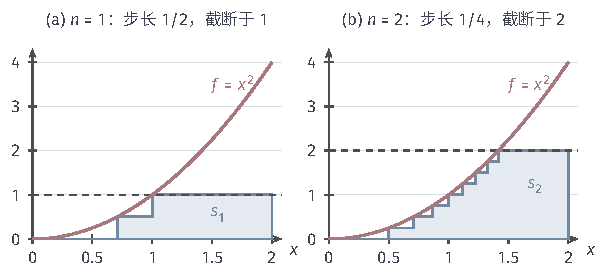
\includegraphics[width=102.634mm]{figures/02-abstract-mathematics/01-metric-and-measure/tikz/c3-dyadic-approximation/figure.pdf}
  \caption{二进分层逼近$f(x)=x^2$，$x\in[0,2]$。蓝色阶梯是$\varphi_n=2^{-n}\lfloor2^n\min\{f,n\}\rfloor$，虚线是截断高度$n$。(a)$n=1$，$\varphi_1$取值$0,0.5,1$；(b)$n=2$，$\varphi_2$取值$0,0.25,\dots,2$，断点为$\sqrt{k/4}$。阶梯始终位于曲线下方，且随$n$增大而升高。}
  \label{fig:meas-dyadic-approximation}
\end{figure}

这个逼近有三点要在下一章用到。第一，它从下方逼近，所以“下方简单函数的累计”自然成为非负函数积分的候选定义。第二，它单调递增，下一章将证明递增逼近的积分收敛到极限的积分。第三，它对每个非负可测函数都存在，不要求连续，也不要求有界；无界或取$+\infty$的函数由截断高度$n$逐步纳入。

\section{本章小结}
\label{sec:meas-summary}

本章开头问：区间里的有理点有多长，挖去无数个中间段后剩下的点集有多长，怎样把“分开测量、合起来相加”推广到这些集合。计数、长度与体积共有的是有限可加性，Jordan测量用有限个矩形从内外夹逼，能处理边界可以用有限个小矩形盖住的集合。有理点集的内外测量分别为$0$与$1$，暴露了有限覆盖的局限；改用可数覆盖，总长度可以任意小。

由此得到两项要求：允许测量的集合族对可数运算封闭，测量规则对可数不交分割可加。$\sigma$代数规定测量范围，生成$\sigma$代数只补入封闭性迫使加入的集合，度量空间的开集生成Borel集，实轴上的区间或半直线已经足够生成它。测度在$\sigma$代数上非负、可数可加，由此推出单调性、可数次可加性与从下连续性；从上连续性需要一个测度有限的起点。零测集与几乎处处说明哪些例外可以忽略，完备化补入零测集的子集而不改变原有集合的测度。

测度的构造分三步。外测度用可数覆盖的最小费用给每个子集赋值，但一般不可加；Carathéodory判据选出与外测度相容的集合，它们构成$\sigma$代数，外测度在其上可数可加。从集合代数上的预测度出发，这一路线给出延拓；延拓的唯一性另需$\sigma$有限条件，并由$\pi$--$\lambda$定理在生成族上比较。

对单调不减且右连续的$F$，区间增量$F(b)-F(a)$确定唯一的Stieltjes测度，跳跃给出点质量；取$F(x)=x$得到Lebesgue测度，它平移不变，其完备化正是Lebesgue可测集。Cantor集零测而不可数，说明测度与基数是两回事；不可测集的存在说明测度只能定义在某个$\sigma$代数上。

有符号测度允许正负值，但至多取一种无穷，以免出现无穷减无穷。Hahn分解把空间切成正集与负集，切法不唯一；Jordan分解把有符号测度写成两个分别集中在不交集合上的测度之差，这个表示唯一且最小。全变差$\lvert\eta\rvert=\eta^++\eta^-$累计正负两方面的质量，也等于有限分割上绝对值之和的上确界，它的零测集正是有符号测度完全看不见的集合。

可测映射用原像规定哪些函数可以用测度研究，只需在生成族上检查；实值函数的可测性归结为阈值集合可测。连续函数都Borel可测，反之不然。可测函数对代数运算和可数次上下确界、上下极限封闭，扩展实值的运算要先说明有定义的范围；零测修改是否保持可测性取决于完备性。

按取值分层得到的递增简单函数列从下方逼近每个非负可测函数，这是第~\ref{chap:integration}章定义积分的出发点。两个测度怎样比较、何时能写成参考测度的加权积分，留到第~\ref{chap:measure-densities}章；质量沿可测映射的转移留到第~\ref{chap:pushforward-measures}章。


\chapter{积分}
\label{chap:integration}

上一章的测度回答“一个集合有多大”。很多问题要的不只是大小，还要求按位置给出不同的贡献再累计：一根细杆各处的线密度不同，总质量是多少；一列函数逐点趋于某个极限，它们的累计是否也趋于极限函数的累计；一个依赖参数的累计量，能不能对参数求导。这些问题的共同对象是测度空间$(X,\mathcal A,\mu)$上的可测函数$f$，要算的是一个数$\int_Xf\,\mathrm d\mu$。

最容易想象的是有限情形。设$X=\{1,\dots,n\}$，第$i$个点的质量是$\mu_i$，函数$f$就是一个数组$[f(1),\dots,f(n)]$。这时累计的意思只有一种：
\[
 \int_Xf\,\mathrm d\mu=\sum_{i=1}^nf(i)\,\mu_i .
\]
它是取值向量与质量向量的内积，对$f$线性，$f\leq g$时结果不减，$f$为某个集合的指示函数时结果就是该集合的测度。本章要把这个加权求和推广到不可数的$X$上，并保留这些性质。

类比到这里遇到困难。$X=[0,1]$时点有不可数多个，每一点的长度都是零，无法逐点相加；而且“先把定义域切成小段”的黎曼做法要求函数在小段上近似常数，这对一般的可测函数不成立。解决办法是改切值域：函数值接近的点归为一层，无论这些点散落在哪里，层的大小都由测度给出。

前三节建立积分本身。第~\ref{sec:integ-definition}节从“层高乘以层的测度”出发，用下方逼近定义非负函数的积分，再用正负部分处理实值函数、用实部虚部处理复值函数。第~\ref{sec:integ-basic-properties}节核对上面那些性质在新定义下的成立条件。第~\ref{sec:integ-classical}节回到熟悉的区间积分，说明黎曼积分与绝对收敛的反常积分怎样被新积分延续，条件收敛的反常积分又为什么不在其列。

后四节研究积分与其他运算能否交换。第~\ref{sec:integ-limits}节从一个积分不随极限收敛的尖峰例子出发，依次证明单调收敛、Fatou估计与支配收敛。第~\ref{sec:integ-iterated}节构造乘积测度，用Tonelli定理与Fubini定理把联合累计拆成依次累计。第~\ref{sec:integ-ftc}节回到区间，研究变上限积分的导数，以及哪些函数能由几乎处处导数的积分恢复。第~\ref{sec:integ-parametric}节把积分看成参数的函数，给出连续性、积分号下求导和变动区域上求导的条件。

本章只使用上一章的测度、可测函数与简单函数逼近。下一章的卷积光滑化与弱导数要用到这里的换序、含参求导与积分恢复。函数列收敛方式的系统比较和一致可积性放在第~\ref{chap:function-normed-spaces}章；用一个测度的加权积分表示另一个测度的问题放在第~\ref{chap:measure-densities}章，沿映射换元放在第~\ref{chap:pushforward-measures}章。

\section{积分的定义}
\label{sec:integ-definition}

黎曼积分把定义域切成小段，在每段上用一个高度近似函数。对有理点的指示函数$\mathbf 1_{\mathbb Q}$，任何小段上都同时有取$0$和取$1$的点，一个高度代表不了这一段。测度提供了另一种切法：按函数值把定义域分层，每一层是一个可测集合，层的高度乘以它的测度，再把各层相加。

图~\ref{fig:integ-slicing-comparison}把两种切法放在同一个函数上对比。左图的小矩形沿横轴并排，每个矩形对应定义域的一小段。右图取定一个值域区间$[t_k,t_{k+1})$，看哪些点的函数值落在其中：这些点在横轴上分成三段，彼此不相邻，却属于同一层。层的贡献只由高度和这三段的总长决定，三段分别在哪里无关紧要。

\begin{BookInlineFigure}
  \centering
  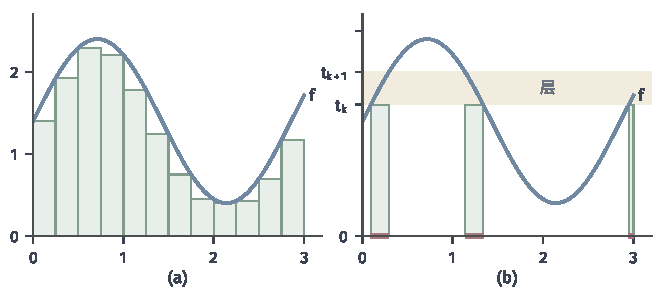
\includegraphics[width=112mm]{figures/04-spaces-measures-and-geometry/02-measure/matplotlib/integ-slicing-comparison/figure.pdf}
  \caption{同一函数$f(x)=1.4+\sin(2.2x)$的两种切法。(a)切定义域：把$[0,3]$等分成$12$段，绿色矩形以各段上$f$的下确界为高。(b)切值域：黄色带是值域区间$[1.6,2.0)$，红色线段是横轴上满足$1.6\leq f<2.0$的点，共三段，绿色矩形以$t_k=1.6$为高画在这些点上。}
  \label{fig:integ-slicing-comparison}
\end{BookInlineFigure}

下面先对只取有限个值的简单函数这样计算，再用简单函数从下方逼近一般的非负可测函数；随后用正负部分处理实值函数，用实部与虚部处理复值函数。

\subsection{非负积分}
\label{sec:integ-nonnegative}

\paragraph{简单函数的积分}
设$(X,\mathcal A,\mu)$是测度空间。非负简单函数在有限个不交可测集合上各取一个常值，分层已经现成，累计的方式就是“高度乘以测度”再求和。

由于测度可以为$+\infty$，先约定$0\cdot(+\infty)=0$：高度为零的层，无论占据多大的集合，贡献都是零。没有这条约定，$\mathbb R$上的零函数就没有积分。

\begin{definition}[非负简单函数的积分]
\label{def:integ-simple}
设$\varphi=\sum_{i=1}^mc_i\mathbf 1_{A_i}$是非负简单函数的标准表示，即$c_1,\dots,c_m\geq0$互不相同，$A_i=\{\varphi=c_i\}$。定义
\begin{equation}
 \int_X\varphi\,\mathrm d\mu=\sum_{i=1}^mc_i\,\mu(A_i)\in[0,+\infty].
 \label{eq:integ-simple}
\end{equation}
\end{definition}

图~\ref{fig:integ-simple-height}中$[0,3]$上的简单函数在$A_1=[0,1)\cup[2,2.5)$上取$2$，在$A_2=[1,2)\cup[2.5,3]$上取$0.5$。两层各占长度$1.5$，所以对Lebesgue测度的积分为
\[
 \int_{[0,3]}\varphi\,\mathrm d\lambda=2\times1.5+0.5\times1.5=3.75 .
\]
图下方的两行线段把两层在横轴上的位置单独画出。每一层都由不相邻的两段组成，而式~\eqref{eq:integ-simple}只用到它们的总长。

\begin{BookInlineFigure}
  \centering
  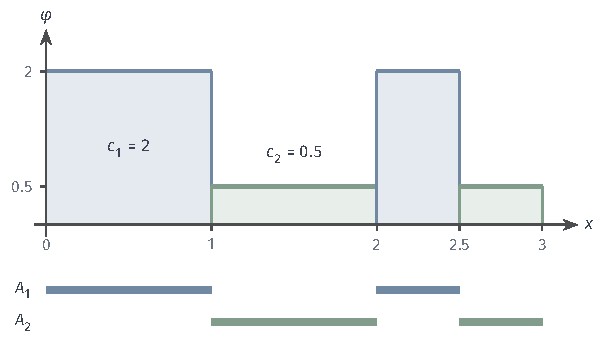
\includegraphics[width=102.401mm]{figures/04-spaces-measures-and-geometry/02-measure/tikz/integ-simple-height/figure.pdf}
  \caption{简单函数积分的“高度乘以测度”。$[0,3]$上的$\varphi$在$A_1=[0,1)\cup[2,2.5)$（蓝）上取$2$，在$A_2=[1,2)\cup[2.5,3]$（绿）上取$0.5$；下方两行线段标出两层占据的集合，各自总长为$1.5$。}
  \label{fig:integ-simple-height}
\end{BookInlineFigure}

同一个简单函数常常以别的方式写出，例如$[0,2]$的指示函数可以拆成$[0,1]$与$(1,2]$两段的指示函数之和。计算时我们希望随手把定义域切成方便的块，不必先合并成标准表示。下面的引理说明这样做得到同一个数，也给出简单函数积分的基本运算。

\begin{lemma}[简单函数积分的运算]
\label{lem:integ-simple-properties}
设$\varphi,\psi$是非负简单函数。
\begin{enumerate}
 \item 若$X$被分成两两不交的可测集$B_1,\dots,B_r$，$\varphi$在$B_j$上取常值$b_j$，则$\int\varphi\,\mathrm d\mu=\sum_jb_j\mu(B_j)$。
 \item 对$a,b\in[0,+\infty)$，有
 \begin{equation}
  \int(a\varphi+b\psi)\,\mathrm d\mu=a\int\varphi\,\mathrm d\mu+b\int\psi\,\mathrm d\mu .
  \label{eq:integ-simple-linear}
 \end{equation}
 \item 若$\varphi\leq\psi$，则$\varphi$的积分不超过$\psi$的积分。
 \item $E\mapsto\int\varphi\mathbf 1_E\,\mathrm d\mu$是$(X,\mathcal A)$上的测度。
\end{enumerate}
\end{lemma}

\begin{proof}
第1条。空的块对右端贡献为零，可以先去掉。设$\varphi$的标准表示为$\sum_ic_i\mathbf 1_{A_i}$，把取同一个值$c_i$的块合并，有
\[
 A_i=\bigcup_{j:\,b_j=c_i}B_j .
\]
由$\mu$的有限可加性，
\[
 \sum_jb_j\mu(B_j)=\sum_ic_i\sum_{j:\,b_j=c_i}\mu(B_j)=\sum_ic_i\mu(A_i).
\]

第2条。设$\varphi$的标准表示以$A_i$为块、取值$\alpha_i$，$\psi$的标准表示以$C_j$为块、取值$\beta_j$。集合$A_i\cap C_j$两两不交、并为$X$，$a\varphi+b\psi$在其上取常值$a\alpha_i+b\beta_j$。由第1条，
\[
 \int(a\varphi+b\psi)\,\mathrm d\mu=\sum_{i,j}(a\alpha_i+b\beta_j)\,\mu(A_i\cap C_j).
\]
把求和拆开，并对固定的$i$用有限可加性$\sum_j\mu(A_i\cap C_j)=\mu(A_i)$，对固定的$j$同样处理，得到
\[
 \int(a\varphi+b\psi)\,\mathrm d\mu=a\sum_i\alpha_i\mu(A_i)+b\sum_j\beta_j\mu(C_j).
\]

第3条。若$\varphi\leq\psi$，则在每个非空的$A_i\cap C_j$上$\alpha_i\leq\beta_j$。按这些块计算两个积分，再逐项比较即得。

第4条。函数$\varphi\mathbf 1_E$在$A_i\cap E$上取$c_i$，在$X\setminus E$上取$0$，由第1条，
\[
 \int\varphi\mathbf 1_E\,\mathrm d\mu=\sum_ic_i\,\mu(A_i\cap E).
\]
右端是有限个测度$E\mapsto\mu(A_i\cap E)$的非负加权和，由上一章的加权和规则，它是测度。
\end{proof}

\paragraph{一般非负函数的积分}
一般的非负可测函数可能取无穷多个值，没有有限分层可以直接计算。可行的办法是从下方逼近：若简单函数$\varphi$满足$0\leq\varphi\leq f$，它的积分就是$f$的累计的一个下界。上一章还证明了存在递增的简单函数列逐点趋于$f$，所以这些下界可以任意接近真正的累计。于是把全部下界的上确界定义为积分。

\begin{definition}[非负可测函数的积分]
\label{def:integ-nonnegative}
设$f:X\to[0,+\infty]$可测。定义
\begin{equation}
 \int_Xf\,\mathrm d\mu=\sup\Bigl\{\int_X\varphi\,\mathrm d\mu:\ \varphi\text{简单},\ 0\leq\varphi\leq f\Bigr\}.
 \label{eq:integ-nonnegative}
\end{equation}
值在$[0,+\infty]$中。常写作$\int f\,\mathrm d\mu$，或在不致混淆时写作$\int f$；对Lebesgue测度也写作$\int f(x)\,\mathrm dx$。
\end{definition}

这个定义与简单函数的积分不冲突。若$f$本身是简单函数，由引理~\ref{lem:integ-simple-properties}第3条，每个下方简单函数的积分都不超过$f$自己的积分，而$f$本身也是候选之一，所以上确界就是$f$自己的积分。

单调性可以直接从定义读出。若$0\leq f\leq g$，每个低于$f$的简单函数也低于$g$，上确界取在更大的范围上，于是$\int f\leq\int g$。

积分允许取$+\infty$。$\mathbb R$上$f\equiv1$的积分对Lebesgue测度为$\lambda(\mathbb R)=+\infty$。$(0,1]$上$f(x)=1/x$的积分也是$+\infty$：简单函数$\sum_{k=1}^nk\mathbf 1_{(1/(k+1),1/k]}$位于$f$下方，因为$(1/(k+1),1/k]$上$1/x\geq k$，而它的积分为
\[
 \sum_{k=1}^nk\Bigl(\frac1k-\frac1{k+1}\Bigr)=\sum_{k=1}^n\frac1{k+1},
\]
随$n$增大而无界。所以“积分有定义”与“积分有限”是两回事：非负函数的积分总有定义，但可能是$+\infty$。

\paragraph{递增逼近的积分}
定义用的是全部下方简单函数的上确界，这是一个庞大的集合。计算时我们只想用一列具体的逼近，例如上一章的二进分层逼近。下面的引理保证这样做不会漏掉任何下界。

\begin{lemma}[递增简单函数列的积分]
\label{lem:integ-increasing-simple}
设$f:X\to[0,+\infty]$可测，$\varphi_1\leq\varphi_2\leq\cdots$是非负简单函数，且对每个$x$有$\lim_n\varphi_n(x)=f(x)$。则
\begin{equation}
 \int_Xf\,\mathrm d\mu=\lim_{n\to\infty}\int_X\varphi_n\,\mathrm d\mu .
 \label{eq:integ-increasing-simple}
\end{equation}
\end{lemma}

\begin{proof}
积分$\int\varphi_n$关于$n$递增，并且都不超过$\int f$，所以极限存在且$\lim_n\int\varphi_n\leq\int f$。反方向要证明：对任意简单函数$0\leq s\leq f$，都有$\lim_n\int\varphi_n\geq\int s$。

固定$c\in(0,1)$，令$E_n=\{\varphi_n\geq cs\}$，它可测且关于$n$递增。下面说明$\bigcup_nE_n=X$。若$s(x)=0$，则$x\in E_1$。若$s(x)>0$，则$f(x)\geq s(x)>cs(x)$，而$\varphi_n(x)\to f(x)$，所以从某项起$\varphi_n(x)\geq cs(x)$。

由于$\varphi_n\geq cs\mathbf 1_{E_n}$，用单调性与线性性得到
\[
 \int\varphi_n\,\mathrm d\mu\geq c\int s\mathbf 1_{E_n}\,\mathrm d\mu .
\]
由引理~\ref{lem:integ-simple-properties}第4条，$E\mapsto\int s\mathbf 1_E\,\mathrm d\mu$是测度，集合$E_n$递增到$X$，所以由测度的从下连续性，右端趋于$c\int s\,\mathrm d\mu$。于是
\[
 \lim_n\int\varphi_n\,\mathrm d\mu\geq c\int s\,\mathrm d\mu .
\]
令$c\uparrow1$，得到所要的不等式。对$s$取上确界，即得$\lim_n\int\varphi_n\geq\int f$。
\end{proof}

引入因子$c<1$是为了处理$f(x)=s(x)$的点：在这些点上$\varphi_n(x)$可能永远略小于$s(x)$，却终究超过$cs(x)$。第~\ref{sec:integ-monotone-convergence}小节用一幅图看这件事，并把同一论证推广到一般的递增可测函数列。

\begin{example}[由定义计算$\int_{[0,1]}x\,\mathrm dx$]
\label{ex:integ-x-dyadic}
取$f(x)=x$，$x\in[0,1]$，测度为Lebesgue测度。二进分层逼近$\varphi_n$在$[k2^{-n},(k+1)2^{-n})$上取$k2^{-n}$，其中$0\leq k<2^n$；点$1$是零测集，在那里的取值不影响积分。每一层的宽度是$2^{-n}$，所以
\[
 \int\varphi_n\,\mathrm d\lambda=\sum_{k=0}^{2^n-1}\frac k{2^n}\cdot\frac1{2^n}=\frac1{4^n}\sum_{k=0}^{2^n-1}k .
\]
用等差数列求和$\sum_{k=0}^{2^n-1}k=\tfrac12(2^n-1)2^n$，得到
\[
 \int\varphi_n\,\mathrm d\lambda=\frac{(2^n-1)2^n}{2\cdot4^n}=\frac12\bigl(1-2^{-n}\bigr).
\]
前三项依次是
\[
 \frac14,\qquad\frac38,\qquad\frac7{16}.
\]
令$n\to\infty$，由引理~\ref{lem:integ-increasing-simple}得$\int_{[0,1]}x\,\mathrm dx=\frac12$，与黎曼积分的值相同。
\end{example}

图~\ref{fig:integ-dyadic-approx}画出了例子中的前三个逼近。绿色面积逐步填满直线下方的三角形。把第$n$步加细到第$n+1$步时，每个台阶右半边抬高$2^{-n-1}$，这些抬高部分的总面积是$2^{-n-2}$，正好是公式$\frac12(1-2^{-n})$的增量。

\begin{BookInlineFigure}
  \centering
  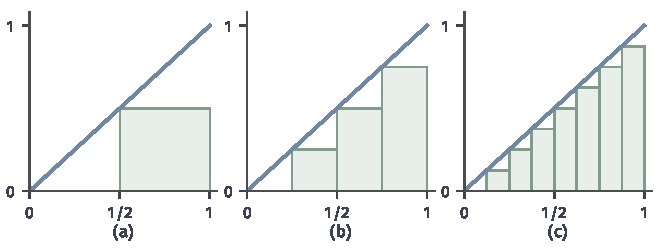
\includegraphics[width=112mm]{figures/04-spaces-measures-and-geometry/02-measure/matplotlib/integ-dyadic-approx/figure.pdf}
  \caption{$f(x)=x$（蓝）的二进分层逼近$\varphi_n$（绿色台阶）。(a)、(b)、(c)依次为$n=1,2,3$，绿色面积分别为$\frac14$、$\frac38$、$\frac7{16}$，递增趋于三角形面积$\frac12$。}
  \label{fig:integ-dyadic-approx}
\end{BookInlineFigure}

\paragraph{非负积分的可加性}
有了递增逼近，加法可以落到简单函数上完成。设$f,g$非负可测，取简单函数列$\varphi_n\uparrow f$与$\psi_n\uparrow g$，例如二进分层逼近。则$\varphi_n+\psi_n$是递增的非负简单函数，逐点收敛到$f+g$。由引理~\ref{lem:integ-increasing-simple}与引理~\ref{lem:integ-simple-properties}第2条，
\begin{equation}
\begin{aligned}
 \int(f+g)\,\mathrm d\mu&=\lim_n\int(\varphi_n+\psi_n)\,\mathrm d\mu\\
 &=\lim_n\int\varphi_n\,\mathrm d\mu+\lim_n\int\psi_n\,\mathrm d\mu\\
 &=\int f\,\mathrm d\mu+\int g\,\mathrm d\mu .
\end{aligned}
 \label{eq:integ-nonnegative-additive}
\end{equation}
用$c\varphi_n\uparrow cf$同样得到$\int cf=c\int f$，其中$c\in[0,+\infty)$。这些等式在$[0,+\infty]$中成立，允许两边为$+\infty$；系数取$+\infty$的情形放在第~\ref{sec:integ-linearity}小节核对。

\subsection{有符号积分}
\label{sec:integ-signed}

\paragraph{正部与负部}
取正负值的函数，正的贡献与负的贡献会相互抵消。若把两者混在一起累计，结果可能取决于累计的先后。最稳妥的做法是把两种贡献分开累计，最后再相减。对可测函数$f:X\to[-\infty,+\infty]$，令
\begin{equation}
 f^+=\max\{f,0\},\qquad f^-=\max\{-f,0\}.
 \label{eq:integ-parts}
\end{equation}
它们是非负可测函数，每一点至少一个为零，并且满足
\[
 f=f^+-f^-,\qquad \lvert f\rvert=f^++f^- .
\]
图~\ref{fig:integ-positive-negative-parts}以$\sin x$为例：$f^+$保留上半部分，$f^-$把下半部分翻到横轴上方。

\begin{BookInlineFigure}
  \centering
  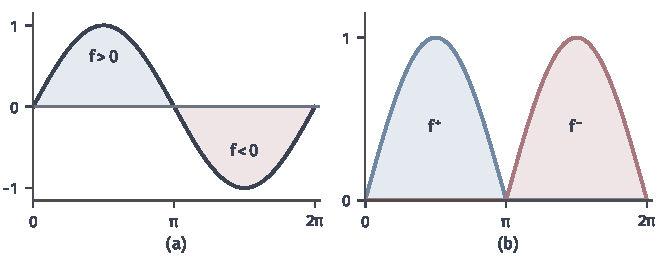
\includegraphics[width=112mm]{figures/04-spaces-measures-and-geometry/02-measure/matplotlib/integ-positive-negative-parts/figure.pdf}
  \caption{正负部分解，$f(x)=\sin x$，$x\in[0,2\pi]$。(a)$f$在$[0,\pi]$上为正（蓝底），在$[\pi,2\pi]$上为负（红底）。(b)正部$f^+$（蓝）与负部$f^-$（红）都是非负函数，每一点至少一个为零。}
  \label{fig:integ-positive-negative-parts}
\end{BookInlineFigure}

分开累计之后，两部分的积分都有意义，唯一的障碍是相减时可能出现$+\infty-(+\infty)$。下面的定义把这种情形排除在外。

\begin{definition}[积分存在与可积]
\label{def:integ-signed}
设$f:X\to[-\infty,+\infty]$可测。若$\int f^+\,\mathrm d\mu$与$\int f^-\,\mathrm d\mu$中至少一个有限，称$f$的积分存在，定义
\begin{equation}
 \int_Xf\,\mathrm d\mu=\int_Xf^+\,\mathrm d\mu-\int_Xf^-\,\mathrm d\mu\in[-\infty,+\infty].
 \label{eq:integ-signed}
\end{equation}
若$\int\lvert f\rvert\,\mathrm d\mu<+\infty$，称$f$关于$\mu$\term{可积}（integrable），也称\term{Lebesgue可积}（Lebesgue integrable），此时积分称为$f$的\term{Lebesgue积分}（Lebesgue integral）。
\end{definition}

三种情形可以这样区分。在$\mathbb R$上取$f=\mathbf 1_{[0,+\infty)}-\mathbf 1_{(-\infty,0)}$，正部与负部的积分都是$+\infty$，$f$的积分不存在；不能因为图像左右对称就说积分为零，那需要额外指定一种抵消的次序。取$f=\mathbf 1_{[0,+\infty)}$，积分存在且等于$+\infty$，但$f$不可积。取$f=\mathbf 1_{[0,1]}-\mathbf 1_{[-2,-1]}$，两部分的积分都是$1$，$f$可积且积分为$0$。

可积性用$\lvert f\rvert$规定，由$\lvert f\rvert=f^++f^-$与式~\eqref{eq:integ-nonnegative-additive}得
\[
 \int\lvert f\rvert\,\mathrm d\mu=\int f^+\,\mathrm d\mu+\int f^-\,\mathrm d\mu .
\]
所以$\int\lvert f\rvert<+\infty$当且仅当两部分的积分都有限。此时$\int f$是有限实数，并且
\[
 \Bigl\lvert\int f\,\mathrm d\mu\Bigr\rvert\leq\int f^+\,\mathrm d\mu+\int f^-\,\mathrm d\mu=\int\lvert f\rvert\,\mathrm d\mu .
\]

\paragraph{零测集与几乎处处等价类}
非负积分对零测集“视而不见”，这是用测度累计的直接后果：零测集这一层，高度再大，贡献也是零。下面的引理把这一点说清楚，并说明积分只依赖函数的几乎处处等价类。

\begin{lemma}[非负积分与零测集]
\label{lem:integ-null-sets}
设$f,g:X\to[0,+\infty]$可测。
\begin{enumerate}
 \item 对$t>0$，$\mu(\{f\geq t\})\leq\frac1t\int f\,\mathrm d\mu$。
 \item 若$\int f\,\mathrm d\mu<+\infty$，则$f<+\infty$几乎处处成立。
 \item $\int f\,\mathrm d\mu=0$当且仅当$f=0$几乎处处成立。
 \item 若$f=g$几乎处处成立，则$\int f\,\mathrm d\mu=\int g\,\mathrm d\mu$。
\end{enumerate}
\end{lemma}

\begin{proof}
第1条。$t\mathbf 1_{\{f\geq t\}}$是低于$f$的简单函数，它的积分是$t\mu(\{f\geq t\})$，所以$t\mu(\{f\geq t\})\leq\int f$。

第2条。对一切$t>0$有$\{f=+\infty\}\subseteq\{f\geq t\}$，由第1条，
\[
 \mu(\{f=+\infty\})\leq\frac1t\int f\,\mathrm d\mu .
\]
令$t\to+\infty$，右端趋于$0$。

第3条。若$\int f=0$，由第1条，对每个正整数$k$有$\mu(\{f\geq1/k\})=0$。又$\{f>0\}=\bigcup_k\{f\geq1/k\}$，所以$\mu(\{f>0\})=0$。反过来，设$N=\{f>0\}$零测。任一低于$f$的简单函数在$N$外为零，它的非零各层都含于$N$，测度为零，所以积分为$0$，上确界也是$0$。

第4条。设$N$是零测集，$f,g$在$N$外相等。对低于$f$的简单函数$\varphi$，函数$\varphi\mathbf 1_{X\setminus N}$低于$g$。由引理~\ref{lem:integ-simple-properties}第4条，
\[
 \int\varphi\,\mathrm d\mu=\int\varphi\mathbf 1_{X\setminus N}\,\mathrm d\mu+\int\varphi\mathbf 1_N\,\mathrm d\mu .
\]
最后一项按层计算为零，所以$\int\varphi\leq\int g$。对$\varphi$取上确界得$\int f\leq\int g$，对称地得到反向不等式。
\end{proof}

第1条称为\term{Markov不等式}（Markov inequality），它用积分控制函数取大值的集合有多大。在$[0,1]$上取$f(x)=x$、$t=\frac12$，左边是$\lambda(\{x\geq\frac12\})=\frac12$，右边是$2\cdot\frac12=1$，不等式成立。

对实值函数，若$f=g$几乎处处成立，则$f^\pm=g^\pm$几乎处处成立，由第4条，两者的积分存在性、可积性和积分值都相同。所以积分是定义在几乎处处等价类上的：在零测集上改动函数，或者在零测集上根本不给函数赋值，都不影响积分。

可积函数的取值可以是$\pm\infty$，但由第2条只能发生在零测集上，因此总可以改成处处取实数值的可积函数而积分不变。把可积函数按几乎处处相等分类，得到的空间及其范数结构在第~\ref{chap:function-normed-spaces}章研究。

\subsection{复值积分}
\label{sec:integ-complex}

\paragraph{复值可测函数的可积性}
Fourier分析中的$e^{\mathrm ikx}$、内积$\int\bar fg$都是复值的，所以积分要推广到复值函数。设$f=u+\mathrm iv:X\to\mathbb C$，其中$u,v$为实值可测函数，上一章已说明$\lvert f\rvert=\sqrt{u^2+v^2}$可测。复数没有正负之分，不能再用正部负部拆开；可以把它看成平面上的向量，分别累计两个坐标，而可积性仍用非负函数$\lvert f\rvert$规定。

\begin{definition}[复值函数的积分]
\label{def:integ-complex}
设$f=u+\mathrm iv$是复值可测函数。若$\int\lvert f\rvert\,\mathrm d\mu<+\infty$，称$f$可积，并定义
\begin{equation}
 \int_Xf\,\mathrm d\mu=\int_Xu\,\mathrm d\mu+\mathrm i\int_Xv\,\mathrm d\mu .
 \label{eq:integ-complex}
\end{equation}
\end{definition}

定义右端要求$u,v$都可积，下面的引理说明这正好由$\lvert f\rvert$可积保证。

\begin{lemma}[复值可积性的等价刻画]
\label{lem:integ-complex-integrable}
复值可测函数$f=u+\mathrm iv$可积，当且仅当$u$与$v$都可积。
\end{lemma}

\begin{proof}
平面上一个向量的长度不小于每个坐标的绝对值，不大于两个坐标绝对值之和，所以逐点有
\[
 \lvert u\rvert\leq\lvert f\rvert,\qquad\lvert v\rvert\leq\lvert f\rvert,\qquad\lvert f\rvert\leq\lvert u\rvert+\lvert v\rvert .
\]
若$\int\lvert f\rvert<+\infty$，由非负积分的单调性，$\int\lvert u\rvert$与$\int\lvert v\rvert$都有限。反过来，由单调性与式~\eqref{eq:integ-nonnegative-additive}，
\[
 \int\lvert f\rvert\,\mathrm d\mu\leq\int\lvert u\rvert\,\mathrm d\mu+\int\lvert v\rvert\,\mathrm d\mu<+\infty.
\]
\end{proof}

\paragraph{共轭与几乎处处相等}
复共轭$\bar f=u-\mathrm iv$与$f$的模相同，所以$\bar f$可积当且仅当$f$可积。由定义~\ref{def:integ-complex}直接得到
\[
 \int\bar f\,\mathrm d\mu=\int u\,\mathrm d\mu-\mathrm i\int v\,\mathrm d\mu=\overline{\int f\,\mathrm d\mu}.
\]
若复值函数$f,g$几乎处处相等，则实部、虚部分别几乎处处相等，由第~\ref{sec:integ-signed}小节，两者的积分相同。所以复值积分同样只依赖几乎处处等价类。

\begin{example}[复值积分的抵消]
\label{ex:integ-complex-cancel}
取$X=\{1,2,3,4\}$，每点质量$1/4$，$f(k)=\mathrm i^k$。实部$u$依次为$0,-1,0,1$，虚部$v$依次为$1,0,-1,0$。分别累计两个坐标：
\[
 \int u\,\mathrm d\mu=\frac14(0-1+0+1)=0,\qquad\int v\,\mathrm d\mu=\frac14(1+0-1+0)=0 .
\]
于是$\int f\,\mathrm d\mu=0$。另一方面$\lvert f\rvert\equiv1$，$\int\lvert f\rvert\,\mathrm d\mu=1$。四个方向的单位复数相互抵消，积分的模远小于模的积分。
\end{example}

复值积分把实值情形的运算搬到两个坐标上，不再比较大小。第~\ref{chap:function-inner-product-spaces}章的$L^2$内积$\langle f,g\rangle=\int f\bar g\,\mathrm d\mu$、第~\ref{chap:fourier-transform}章的Fourier系数与Fourier变换，都以这里的复值积分及其共轭规则为共同运算。

\section{积分的基本性质}
\label{sec:integ-basic-properties}

计算积分时我们反复做三件事：把被积函数拆成几项分别积分，用一个容易计算的函数从上方或下方比较，把积分区域切成几块分别累计。在有限情形$\sum_if(i)\mu_i$里，这三件事分别对应求和的线性、逐项比较和分组求和，都没有条件。

积分的情形多了一个麻烦：值可以是$+\infty$，而$+\infty-(+\infty)$没有意义。所以下面每条规则都要写明范围：可积函数的运算在有限实数中进行，非负函数允许积分为$+\infty$，但不允许系数为负。

\subsection{线性性}
\label{sec:integ-linearity}

\paragraph{三种情形的线性性}
线性性要回答两件事：线性组合是否仍属于可以积分的范围，积分能否逐项计算。非负函数总可以积分，但系数必须非负，否则会产生负值；可积函数允许任意实系数或复系数，代价是要先核对线性组合仍然可积。

\begin{theorem}[积分的线性性]
\label{thm:integ-linearity}
\begin{enumerate}
 \item 设$f,g:X\to[0,+\infty]$可测，$a,b\in[0,+\infty]$，约定$0\cdot(+\infty)=0$。则下式在$[0,+\infty]$中成立：
 \begin{equation}
  \int(af+bg)\,\mathrm d\mu=a\int f\,\mathrm d\mu+b\int g\,\mathrm d\mu .
  \label{eq:integ-linearity}
 \end{equation}
 \item 设$f,g$是实值可积函数，$a,b\in\mathbb R$。则$af+bg$可积，且式~\eqref{eq:integ-linearity}成立。
 \item 设$f,g$是复值可积函数，$a,b\in\mathbb C$。则$af+bg$可积，且式~\eqref{eq:integ-linearity}成立。
\end{enumerate}
\end{theorem}

\begin{proof}
第1条。由式~\eqref{eq:integ-nonnegative-additive}，$\int(af+bg)=\int af+\int bg$，所以只需证明$\int af=a\int f$。系数有限的情形第~\ref{sec:integ-nonnegative}小节已经给出，只需处理$a=+\infty$。

函数$(+\infty)\cdot f$在$\{f>0\}$上取$+\infty$，在$\{f=0\}$上取$0$。分两种情形。若$\mu(\{f>0\})>0$，这个函数的积分为$+\infty$；由引理~\ref{lem:integ-null-sets}第3条，此时$\int f>0$，右端$(+\infty)\cdot\int f$也是$+\infty$。若$\mu(\{f>0\})=0$，左端是几乎处处为零的函数的积分，等于$0$；右端是$(+\infty)\cdot0=0$。

第2条，先看可积性。可积函数只在零测集上取$\pm\infty$，把这些点上的值改成$0$，积分不变，$af+bg$处处有定义。由三角不等式与第1条，
\[
 \int\lvert af+bg\rvert\,\mathrm d\mu\leq\lvert a\rvert\int\lvert f\rvert\,\mathrm d\mu+\lvert b\rvert\int\lvert g\rvert\,\mathrm d\mu<+\infty,
\]
所以$af+bg$可积。

再看数乘。$a\geq0$时$(af)^\pm=af^\pm$；$a<0$时$(af)^+=\lvert a\rvert f^-$，$(af)^-=\lvert a\rvert f^+$。代入式~\eqref{eq:integ-signed}，两种情形都得到$\int af=a\int f$。

最后看加法。令$h=f+g$。把$h^+-h^-=f^+-f^-+g^+-g^-$中带负号的项移到另一边，得到
\[
 h^++f^-+g^-=h^-+f^++g^+ .
\]
两边都是非负可测函数之和，由第1条逐项积分，六个积分都有限，于是可以移项，得到
\[
 \int h\,\mathrm d\mu=\int f\,\mathrm d\mu+\int g\,\mathrm d\mu .
\]

第3条。第2条中的三角不等式对复数同样成立，给出可积性。加法按实部与虚部分别用第2条。对复数$a=\alpha+\mathrm i\beta$与$f=u+\mathrm iv$，有
\[
 af=(\alpha u-\beta v)+\mathrm i(\alpha v+\beta u).
\]
由第2条分别积分实部与虚部，再合并成复数的乘积：
\[
\begin{aligned}
 \int af&=\alpha\int u-\beta\int v+\mathrm i\Bigl(\alpha\int v+\beta\int u\Bigr)\\
 &=(\alpha+\mathrm i\beta)\Bigl(\int u+\mathrm i\int v\Bigr)=a\int f.
\end{aligned}
\]
\end{proof}

\paragraph{条件不能省略}
第2条要求两个函数都可积，只知道各自的积分存在是不够的。在$\mathbb R$上取$f\equiv1$、$g\equiv-1$，两者的积分分别为$+\infty$与$-\infty$，都存在。而$f+g\equiv0$的积分为$0$，右端却是$+\infty+(-\infty)$，没有意义。

第1条要求系数非负，同样是为了不让正负贡献相遇。由第2条，可积函数全体对线性组合封闭，积分是其上的线性映射，就像有限维时$f\mapsto\sum_if(i)\mu_i$是一个线性函数。这一结构在第~\ref{chap:function-normed-spaces}章作为函数空间再研究。

\subsection{单调性}
\label{sec:integ-monotonicity}

\paragraph{逐点比较}
用一个已知的函数控制被积函数，是估计积分最常用的办法。非负函数的单调性已由定义得到；对实值可积函数，比较可以借助线性性完成：$f\leq g$意味着$g-f\geq0$，非负函数的积分非负。

\begin{theorem}[积分的单调性]
\label{thm:integ-monotonicity}
设$f,g$都是非负可测函数，或都是实值可积函数。若$f\leq g$几乎处处成立，则$\int f\,\mathrm d\mu\leq\int g\,\mathrm d\mu$。若还有$\int f=\int g$且两者有限，则$f=g$几乎处处成立。
\end{theorem}

\begin{proof}
设$N$是零测集，$f\leq g$在$N$外成立。把$f,g$在$N$上都改成$0$，由引理~\ref{lem:integ-null-sets}第4条（实值情形对正负部分别使用），积分不变，而改后的函数处处满足$f\leq g$。

非负情形由定义的单调性得结论。可积情形中，$g-f$是几乎处处非负的可积函数，由线性性，
\[
 \int g\,\mathrm d\mu-\int f\,\mathrm d\mu=\int(g-f)\,\mathrm d\mu\geq0 .
\]

现在设两个积分相等且有限。非负情形下$f,g$的积分有限，也属于可积函数，所以统一按可积情形处理。这时$\int(g-f)=0$，而$g-f$几乎处处非负，由引理~\ref{lem:integ-null-sets}第3条，$g-f=0$几乎处处成立。
\end{proof}

逐点不等式放宽到几乎处处，是因为积分看不见零测集上的取值。例如在$[0,1]$上，$\mathbf 1_{\mathbb Q}\leq0$只在零测的有理点之外成立，结论$\int\mathbf 1_{\mathbb Q}\leq0$仍然正确，再结合$\mathbf 1_{\mathbb Q}\geq0$，得$\int\mathbf 1_{\mathbb Q}=0$。

\paragraph{复值积分不比较大小}
复数之间没有与运算相容的次序，所以复值积分没有单调性可言。能比较的是实值量：实部与虚部满足$\operatorname{Re}\int f=\int\operatorname{Re}f$，可以对它们分别使用单调性；模$\lvert f\rvert$是非负函数，也可以比较。下一小节就是用实部与模的比较来估计复值积分。

\subsection{积分的绝对值估计}
\label{sec:integ-absolute-estimate}

\paragraph{实值与复值情形}
积分是加权累计，取绝对值之后，正负或不同方向的贡献不再抵消，累计只会变大。这与向量的三角不等式$\lVert\sum_iv_i\rVert\leq\sum_i\lVert v_i\rVert$是同一件事：把许多向量首尾相接，总位移不超过路程之和。

\begin{theorem}[积分的绝对值估计]
\label{thm:integ-absolute-estimate}
设$f$是实值或复值可积函数，则
\begin{equation}
 \Bigl\lvert\int f\,\mathrm d\mu\Bigr\rvert\leq\int\lvert f\rvert\,\mathrm d\mu .
 \label{eq:integ-absolute-estimate}
\end{equation}
\end{theorem}

\begin{proof}
实值情形。由$-\lvert f\rvert\leq f\leq\lvert f\rvert$与单调性、线性性，
\[
 -\int\lvert f\rvert\,\mathrm d\mu\leq\int f\,\mathrm d\mu\leq\int\lvert f\rvert\,\mathrm d\mu .
\]

复值情形。记$z=\int f\,\mathrm d\mu$。若$z=0$，左端为零，不等式成立。若$z\neq0$，令$\alpha=\bar z/\lvert z\rvert$，这是模为一的复数，使$\alpha z=\lvert z\rvert$为正实数。由复线性性，
\[
 \lvert z\rvert=\alpha\int f\,\mathrm d\mu=\int\alpha f\,\mathrm d\mu .
\]
左边是实数，所以它等于右边的实部。再用复数的实部不超过它的模这一事实与单调性，并利用$\lvert\alpha\rvert=1$，得到
\[
 \lvert z\rvert=\int\operatorname{Re}(\alpha f)\,\mathrm d\mu\leq\int\lvert\alpha f\rvert\,\mathrm d\mu=\int\lvert f\rvert\,\mathrm d\mu .
\]
\end{proof}

证明中乘以$\alpha$的作用是把积分旋转到正实轴上，这样复数的模就变成了可以比较大小的实部。例~\ref{ex:integ-complex-cancel}中$\lvert\int f\rvert=0<1=\int\lvert f\rvert$，说明不等式可以严格成立：四个向量首尾相接回到原点，总位移为零，路程却是$1$。

\paragraph{误差控制}
把估计用于两个可积函数之差，就得到积分误差的界：
\begin{equation}
 \Bigl\lvert\int f\,\mathrm d\mu-\int g\,\mathrm d\mu\Bigr\rvert\leq\int\lvert f-g\rvert\,\mathrm d\mu .
 \label{eq:integ-error-bound}
\end{equation}
用$g$近似$f$时，积分结果的误差不超过两者差的模的积分。

用例~\ref{ex:integ-x-dyadic}的二进分层函数检验这个界。在$[0,1]$上用$\varphi_n$近似$f(x)=x$，逐点有$0\leq f-\varphi_n\leq2^{-n}$，所以式~\eqref{eq:integ-error-bound}的右端不超过$2^{-n}$。实际误差是
\[
 \frac12-\frac12\bigl(1-2^{-n}\bigr)=2^{-n-1},
\]
确实在这个界之内。第~\ref{sec:integ-dominated-convergence}小节将用同一个量$\int\lvert f_n-f\rvert$判断一列近似的积分是否收敛。

\subsection{积分区域的可加性}
\label{sec:integ-domain-additivity}

\paragraph{子集上的积分}
在可测子集$A$上积分，就是只累计$A$内的贡献。用指示函数把$A$外的值清零，就可以沿用全空间上的定义。

\begin{definition}[可测子集上的积分]
\label{def:integ-subset}
设$A\in\mathcal A$，$f$非负可测或可积。定义
\begin{equation}
 \int_Af\,\mathrm d\mu=\int_Xf\mathbf 1_A\,\mathrm d\mu .
 \label{eq:integ-subset}
\end{equation}
对Lebesgue测度和区间$A=[a,b]$，也写作$\int_a^bf(x)\,\mathrm dx$。
\end{definition}

这个积分也等于把$f$限制到$A$上、在$A$的可测子集族上对$\mu$所作的积分，因为两种算法在简单函数上逐层相同，再由递增逼近推广到一般函数。若$f$可积，由$\lvert f\mathbf 1_A\rvert\leq\lvert f\rvert$，$f$在每个可测子集上可积。

\paragraph{有限拆分与零测集}
设$A,B\in\mathcal A$不交。则$f\mathbf 1_{A\cup B}=f\mathbf 1_A+f\mathbf 1_B$，由线性性，
\begin{equation}
 \int_{A\cup B}f\,\mathrm d\mu=\int_Af\,\mathrm d\mu+\int_Bf\,\mathrm d\mu .
 \label{eq:integ-domain-additive}
\end{equation}
这对非负可测函数在$[0,+\infty]$中成立，对可积函数在有限数中成立；归纳可得有限个不交区域的情形。

若$N$是零测集，$f\mathbf 1_{A\cup N}$与$f\mathbf 1_A$只在$N$上可能不同，所以$\int_{A\cup N}f=\int_Af$。增删零测集不改变积分，区间端点开闭也就无关紧要：$\int_{[a,b]}f=\int_{(a,b)}f$。

\paragraph{可数拆分}
可数个不交区域$A_1,A_2,\dots$的情形不能从有限拆分直接得到，因为需要交换积分与无限求和。对非负可测函数，第~\ref{sec:integ-monotone-convergence}小节的单调收敛定理将给出
\begin{equation}
 \int_{\bigcup_nA_n}f\,\mathrm d\mu=\sum_n\int_{A_n}f\,\mathrm d\mu,
 \label{eq:integ-domain-countable}
\end{equation}
两边允许为$+\infty$；对可积函数，再由支配收敛得到同样的等式且级数绝对收敛。换句话说，对非负可测函数$f$，$A\mapsto\int_Af\,\mathrm d\mu$本身是一个测度。由非负函数生成的这类测度怎样反过来刻画，放在第~\ref{chap:measure-densities}章。

\section{与经典积分的关系}
\label{sec:integ-classical}

新积分的定义与黎曼积分完全不同：一个切值域，一个切定义域。对熟悉的区间积分，两种定义给出的数是否相同，新积分又多处理了哪些函数？

本节分两种情形比较。有界闭区间上的有界函数，用不连续点集刻画黎曼可积性并证明两种积分相等；无界区间或奇点附近的反常积分，绝对收敛时与新积分一致，条件收敛时则不然。下文中区间上的测度都是Lebesgue测度$\lambda$。

\subsection{与黎曼积分的关系}
\label{sec:integ-riemann}

\paragraph{阶梯函数与上下和}
两种理论的接触点是阶梯函数。对区间$I\subseteq[a,b]$，$\int\mathbf 1_I\,\mathrm d\lambda=\lambda(I)$等于区间长度，与黎曼积分的值相同；端点是零测集，开闭不影响Lebesgue积分。由线性性，阶梯函数$\sum_ic_i\mathbf 1_{I_i}$的两种积分都等于$\sum_ic_i\lambda(I_i)$。而黎曼积分的上和与下和正是阶梯函数的积分，两种理论就从这里连起来。

回顾卷一的Darboux判据：有界函数$f$在$[a,b]$上黎曼可积，当且仅当对任意$\varepsilon>0$存在分割$P$，使上和与下和之差$U(f,P)-L(f,P)<\varepsilon$；此时黎曼积分是上下和共同逼近的值（可参考\BookChapterRef{chap:univariate-integration}{卷一第7章“一元函数的积分”}）。下面的判据把“上下和之差可以任意小”换成一个关于不连续点的测度条件。

\paragraph{振幅与不连续点}
上下和之差由函数在小段上的跳动幅度决定，所以要先量化函数在一点附近的跳动。设$f:[a,b]\to\mathbb R$有界，记$I_\delta(x)=(x-\delta,x+\delta)\cap[a,b]$，定义$f$在$x$处的\term{振幅}（oscillation）
\begin{equation}
 \omega_f(x)=\inf_{\delta>0}\Bigl(\sup_{I_\delta(x)}f-\inf_{I_\delta(x)}f\Bigr).
 \label{eq:integ-oscillation}
\end{equation}
括号内的量随$\delta$减小而不增，下确界就是$\delta\downarrow0$时的极限。$f$在$x$连续当且仅当$\omega_f(x)=0$，所以不连续点集为$D_f=\bigcup_{m\geq1}\{\omega_f\geq1/m\}$。例如$\mathbf 1_{[1/2,1]}$在$x=\frac12$处的振幅是$1$，在其余点都是$0$。

有了振幅，可以陈述下面的判据：决定黎曼可积性的是不连续点集的测度。

\begin{theorem}[黎曼可积的Lebesgue判据]
\label{thm:integ-riemann-lebesgue}
设$f:[a,b]\to\mathbb R$有界。$f$黎曼可积，当且仅当其不连续点集$D_f$是Lebesgue零测集。此时$f$关于Lebesgue可测集可测，Lebesgue可积，且$\int_{[a,b]}f\,\mathrm d\lambda$等于$f$的黎曼积分。
\end{theorem}

这一判据称为\term{Lebesgue判据}（Lebesgue criterion）。证明分三步：先说明黎曼可积函数被两列阶梯函数夹住，由此得到两种积分相等；再读出$D_f$零测；最后由$D_f$零测构造上下和之差很小的分割。下面始终记$\lvert f\rvert\leq M$。

\begin{proof}
\emph{第一步：两种积分相等。}设$f$黎曼可积。由Darboux判据，对每个$k$有分割$Q_k$使上下和之差小于$1/k$。令$P_k$为$Q_1,\dots,Q_k$的公共加细，加细不增大上下和之差，于是$P_1\subseteq P_2\subseteq\cdots$，且$U(f,P_k)-L(f,P_k)\to0$。

对$P_k$的每个小段$[x_{i-1},x_i]$，记$m_i,M_i$为$f$在其上的下、上确界，令$J_i=[x_{i-1},x_i)$（最后一段取闭区间），定义阶梯函数
\[
 \varphi_k=\sum_im_i\mathbf 1_{J_i},\qquad\psi_k=\sum_iM_i\mathbf 1_{J_i}.
\]
于是$\varphi_k\leq f\leq\psi_k$，并且
\[
 \int\varphi_k\,\mathrm d\lambda=L(f,P_k),\qquad\int\psi_k\,\mathrm d\lambda=U(f,P_k).
\]

分割加细时子段上的下确界不减、上确界不增，所以$\varphi_k$递增、$\psi_k$递减，分别有逐点极限$\varphi\leq f\leq\psi$，它们都是Borel可测函数。由$0\leq\psi-\varphi\leq\psi_k-\varphi_k$，得到
\[
 \int(\psi-\varphi)\,\mathrm d\lambda\leq U(f,P_k)-L(f,P_k)\to0 .
\]
所以$\psi=\varphi$在某个零测集$N$外成立，从而$f=\varphi$在$N$外成立。

集合$\{f>t\}$与Borel集$\{\varphi>t\}$只在$N$内可能不同，Lebesgue测度完备，所以$f$关于$\mathcal L$可测；又$\lvert f\rvert\leq M$，$f$在有限长区间上可积。$\varphi_k+M$是递增的非负简单函数，逐点收敛到$\varphi+M$，由引理~\ref{lem:integ-increasing-simple}，$\int(\varphi_k+M)\to\int(\varphi+M)$。两边减去有限数$M(b-a)$，得到
\[
 \int_{[a,b]}f\,\mathrm d\lambda=\int_{[a,b]}\varphi\,\mathrm d\lambda=\lim_kL(f,P_k)=\int_a^bf(x)\,\mathrm dx .
\]

\emph{第二步：$D_f$零测。}全部分割$P_k$的分点只有可数个，组成零测集$Z$。若$x\notin Z$，对每个$k$，$x$位于$P_k$某个小段的内部，存在$\delta$使$I_\delta(x)$含于该小段，于是
\[
 \omega_f(x)\leq M_i-m_i=\psi_k(x)-\varphi_k(x).
\]
令$k\to\infty$得$\omega_f(x)\leq\psi(x)-\varphi(x)$。在零测集$Z\cup N$之外右端为零，所以$D_f\subseteq Z\cup N$是零测集。

\emph{第三步：$D_f$零测蕴含黎曼可积。}给定$\varepsilon>0$，令$K=\{\omega_f\geq\varepsilon\}$。$K$是闭集：若$\omega_f(x)<\varepsilon$，取$\delta$使$I_\delta(x)$上上下确界之差小于$\varepsilon$，则对$\lvert y-x\rvert<\delta/2$有$I_{\delta/2}(y)\subseteq I_\delta(x)$，故$\omega_f(y)<\varepsilon$。

$K\subseteq D_f$是零测的有界闭集，可用可数个开区间覆盖且总长小于$\varepsilon$。$K$紧，取其中有限个，其并$G$由有限个不交开区间组成，总长小于$\varepsilon$。于是$[a,b]\setminus G$是有限个闭区间$H_1,\dots,H_r$之并，其上处处$\omega_f<\varepsilon$。

对每点$x\in H_l$取$\delta_x$，使$I_{\delta_x}(x)$上上下确界之差小于$\varepsilon$。区间$(x-\delta_x/2,x+\delta_x/2)$覆盖紧集$H_l$，取有限子覆盖，令$\delta$为相应$\delta_x/2$的最小值。若$H_l$中的小段$J$长度小于$\delta$，它含于某个$I_{\delta_x}(x)$，$f$在$J$上的上下确界之差小于$\varepsilon$。

把每个$H_l$分成长度小于$\delta$的小段，再加上$G$各分支的端点，得到分割$P$。上下和之差分两部分估计：落在某个$H_l$中的小段，每段的上下确界之差小于$\varepsilon$，总长不超过$b-a$，贡献小于$\varepsilon(b-a)$；落在$G$某个分支闭包中的小段，上下确界之差至多$2M$，总长小于$\varepsilon$，贡献至多$2M\varepsilon$。于是
\[
 U(f,P)-L(f,P)<\varepsilon(b-a+2M),
\]
由Darboux判据，$f$黎曼可积。
\end{proof}

第一步说明两种理论在共同范围内一致：黎曼可积函数的上下阶梯函数从两侧夹住它，Lebesgue积分记录了夹逼的公共极限。第二、三步说明黎曼可积的障碍恰好是不连续点占据正的长度。

这里用到了完备性。黎曼可积函数未必Borel可测，但与一个Borel函数只在零测集上不同，所以结论说的是关于Lebesgue可测集$\mathcal L$可测。

\paragraph{有理点指示函数}
在$[0,1]$上，有理点的指示函数$\mathbf 1_{\mathbb Q}$称为\term{Dirichlet函数}（Dirichlet function）。$\mathbb Q\cap[0,1]$可数，Lebesgue测度为零，所以
\[
 \int_{[0,1]}\mathbf 1_{\mathbb Q}\,\mathrm d\lambda=0 .
\]
另一方面，每个小区间上它的上确界为$1$、下确界为$0$，振幅处处为$1$，$D_f=[0,1]$的测度为$1$，所以它不黎曼可积。这与“任意分割的下和为$0$、上和为$1$”的直接计算一致。

图~\ref{fig:integ-dirichlet-function}把这个例子与Cantor集的指示函数放在一起。Cantor集$C$是零测的闭集，$\mathbf 1_C$在每个$x\notin C$的邻域内恒为零，因而连续；在$x\in C$处，由于$C$不含任何区间，$x$附近有取值为零的点，因而不连续。于是$D_f=C$不可数却零测，$\mathbf 1_C$黎曼可积，两种积分都是$0$。

\begin{BookInlineFigure}
  \centering
  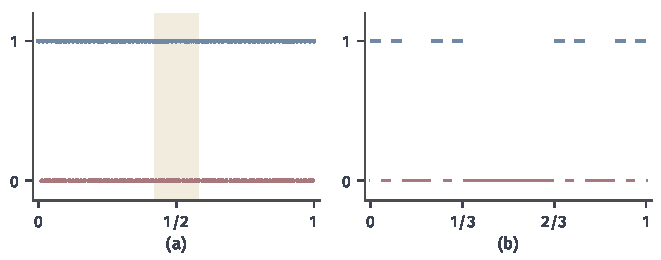
\includegraphics[width=112mm]{figures/04-spaces-measures-and-geometry/02-measure/matplotlib/integ-dirichlet-function/figure.pdf}
  \caption{两种不连续点集。(a)Dirichlet函数在有理点取$1$（蓝点）、无理点取$0$（红点），图中各取若干代表；两类点都稠密，任一小区间（黄色带）上上确界为$1$、下确界为$0$，不连续点集为整个$[0,1]$。(b)Cantor集的指示函数$\mathbf 1_C$，用第三步的$8$个保留区间示意$C$：蓝色线段处取$1$，红色线段处取$0$。它只在$C$上不连续，$\lambda(C)=0$，所以黎曼可积。}
  \label{fig:integ-dirichlet-function}
\end{BookInlineFigure}

两张图的对比说明，决定黎曼可积性的是不连续点集的测度，而不是它的基数或稠密性。$\mathbb Q$的基数比$C$小，$\mathbf 1_{\mathbb Q}$却不黎曼可积，因为它的不连续点集是全区间。Lebesgue积分则根本不要求函数在小区间上近似为常数，只要求各层可测。

\subsection{与反常积分的关系}
\label{sec:integ-improper}

\paragraph{截断区间的极限}
反常积分处理两种情形：区间无界，或函数在端点附近无界。做法都是先在有限闭区间上作黎曼积分，再让区间扩张取极限。新积分则直接在整个区间上累计，不需要截断。对非负函数，截断区间上的积分随区间扩张递增，这正是下一节单调收敛定理处理的情形。

\begin{theorem}[反常积分与Lebesgue积分]
\label{thm:integ-improper}
设$-\infty<a<\beta\leq+\infty$，$I=[a,\beta)$，$f:I\to\mathbb R$在每个$[a,b]$（$a<b<\beta$）上黎曼可积。
\begin{enumerate}
 \item 若$f\geq0$，则下式在$[0,+\infty]$中成立：
 \begin{equation}
  \int_If\,\mathrm d\lambda=\lim_{b\uparrow\beta}\int_a^bf(x)\,\mathrm dx .
  \label{eq:integ-improper}
 \end{equation}
 \item $f$在$I$上Lebesgue可积，当且仅当反常积分$\int_a^\beta\lvert f(x)\rvert\,\mathrm dx$收敛，即$\int_a^\beta f$绝对收敛；此时$\int_If\,\mathrm d\lambda$等于反常积分$\int_a^\beta f(x)\,\mathrm dx$。
\end{enumerate}
左端点为奇点的区间$(\alpha,b]$与两端都需截断的区间可类似处理。
\end{theorem}

证明的机制是：取$b_n\uparrow\beta$，截断函数$f\mathbf 1_{[a,b_n]}$逐点收敛到$f\mathbf 1_I$；当$f\geq0$时这列函数递增，积分与极限可以交换，而每个截断积分由定理~\ref{thm:integ-riemann-lebesgue}等于黎曼积分。交换的依据是单调收敛定理，所以完整证明放在第~\ref{sec:integ-monotone-convergence}小节，作为它的第一个应用。

对非负函数，反常积分收敛与Lebesgue可积是同一回事，值也相同。下面两个积分分别对应端点奇性和无界区间：
\[
\begin{aligned}
 \int_{(0,1]}x^{-1/2}\,\mathrm dx&=\lim_{\varepsilon\downarrow0}\bigl(2-2\sqrt\varepsilon\bigr)=2,\\
 \int_{[1,+\infty)}x^{-2}\,\mathrm dx&=\lim_{b\to+\infty}\Bigl(1-\frac1b\Bigr)=1 .
\end{aligned}
\]
对可正可负的函数，两种理论只在绝对收敛时一致；复值函数对实部和虚部分别使用第2条。

\paragraph{条件收敛不足以保证可积}
反常积分只要求截断积分有极限，允许正负部分相互抵消；Lebesgue积分则要求正负两部分各自有限。$f(x)=\sin x/x$在$[1,+\infty)$上体现了这一区别，图~\ref{fig:integ-sinc-improper}画出了它的前几瓣。

先看反常积分。分部积分得到
\[
 \int_1^b\frac{\sin x}x\,\mathrm dx=\cos1-\frac{\cos b}b-\int_1^b\frac{\cos x}{x^2}\,\mathrm dx .
\]
$b\to+\infty$时，$\cos b/b\to0$，而$\lvert\cos x/x^2\rvert\leq1/x^2$在$[1,+\infty)$上可积，最后一项也有有限极限。所以反常积分存在。

再看绝对值。在第$k$瓣$[k\pi,(k+1)\pi]$（$k\geq1$）上，$1/x\geq1/((k+1)\pi)$，而$\lvert\sin x\rvert$在每一瓣上的积分都是$2$，所以
\[
 \int_{[1,+\infty)}\frac{\lvert\sin x\rvert}x\,\mathrm dx\geq\sum_{k=1}^\infty\frac2{(k+1)\pi}=+\infty .
\]
由定理~\ref{thm:integ-improper}，$f$不Lebesgue可积。

进一步，$\int f^+$与$\int f^-$都是$+\infty$。它们是$\int_1^bf^\pm$的极限，而$\int_1^bf^+-\int_1^bf^-$有有限极限；若其中一个有限，另一个也有限，与$\int\lvert f\rvert=+\infty$矛盾。因此$f$在$[1,+\infty)$上的Lebesgue积分不存在。

\begin{BookInlineFigure}
  \centering
  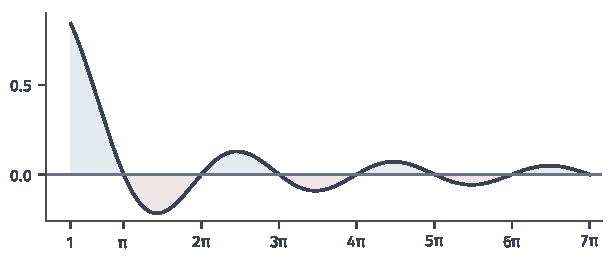
\includegraphics[width=104mm]{figures/04-spaces-measures-and-geometry/02-measure/matplotlib/integ-sinc-improper/figure.pdf}
  \caption{$f(x)=\sin x/x$在$[1,7\pi]$上的图像，正瓣蓝底、负瓣红底。第$k$瓣$[k\pi,(k+1)\pi]$上$\lvert f\rvert$的面积不小于$2/((k+1)\pi)$，各瓣面积之和按调和级数发散。按$x$增大的次序累加时正负瓣相互抵消，反常积分收敛。}
  \label{fig:integ-sinc-improper}
\end{BookInlineFigure}

图中正瓣与负瓣交替出现，面积按$1/k$缓慢减小。反常积分按从左到右的次序累加，正负瓣两两抵消，部分和收敛；把正瓣和负瓣分别累加，各自都发散。这与条件收敛的数项级数$\sum(-1)^k/k$相同：它的值依赖求和的次序。

测度积分不使用任何次序，所以它只接受与次序无关的绝对收敛情形。这并不是新积分的缺陷：需要条件收敛积分的场合，仍可以把它写成Lebesgue积分在截断区间上的极限。

\section{积分与极限}
\label{sec:integ-limits}

分析中的许多函数是逐步逼近得到的：级数的部分和、截断区间上的函数、越来越细的平均。若一列可测函数逐点趋于目标函数，我们希望各次积分也趋于目标函数的积分，这样就能用容易计算的近似求出难以直接计算的积分。本节先说明逐点与几乎处处收敛的含义，用一个尖峰例子说明交换不能无条件进行；再依次研究递增逼近、非负函数列的下极限估计，以及由同一个可积函数控制的函数列。收敛方式的系统比较以及一致可积性，留到第~\ref{chap:normed-spaces}章。

\subsection{逐点逼近与积分极限}
\label{sec:integ-pointwise}

\paragraph{逐点收敛与几乎处处收敛}
固定一个输入点$x$，函数列$f_1,f_2,\dots$在这一点的取值是一列数$f_1(x),f_2(x),\dots$。若对每个$x\in X$，这列数都收敛到$f(x)$，称$f_n$\term{逐点收敛}（pointwise convergence）到$f$。积分看不见零测集，所以只需要求收敛在零测集之外成立：若存在零测集$N$，使$f_n(x)\to f(x)$对每个$x\notin N$成立，称$f_n$\term{几乎处处收敛}（almost everywhere convergence）到$f$。

几乎处处的极限只确定到零测集。若$f_n$几乎处处收敛到$f$与$g$，两个例外集之并仍是零测集，在它之外$f=g$，所以$f=g$几乎处处成立。极限函数的可测性也要留意：收敛点集$\{x:\limsup_nf_n(x)=\liminf_nf_n(x)\}$可测，在其上取$\limsup_nf_n$、其外取$0$，就得到一个可测的极限代表；在完备测度空间中，任何几乎处处等于它的函数都可测。下面谈到几乎处处收敛的极限时，总指这样一个可测代表。

\paragraph{积分不随逐点极限收敛的例子}
在$[0,1]$上取
\[
 f_n(x)=n\mathbf 1_{(0,1/n)}(x),\qquad n\geq1.
\]
对$x=0$，每个$f_n(0)=0$；对$x>0$，当$n>1/x$时$x\notin(0,1/n)$，$f_n(x)=0$。所以$f_n$逐点收敛到$0$。但每个$f_n$是高为$n$、宽为$1/n$的矩形，$\int f_n=1$，于是
\[
 \lim_{n\to\infty}\int_{[0,1]}f_n\,\mathrm d\lambda=1\neq0=\int_{[0,1]}\lim_{n\to\infty}f_n\,\mathrm d\lambda .
\]
质量没有消失，而是挤进了越来越窄的区间：每一点最终都看不到尖峰，尖峰的面积却始终是$1$。这说明积分与极限的交换需要条件。下面三小节给出三种条件：函数列递增，函数列非负（只得到单向估计），以及函数列被一个可积函数共同控制。

\subsection{单调收敛}
\label{sec:integ-monotone-convergence}

\paragraph{单调收敛定理}
尖峰例子中的函数列不单调：$f_n$在$(0,1/n)$上增大，在别处变为零。若函数列递增，质量只会不断加入，不会挤走，积分就能与极限交换。引理~\ref{lem:integ-increasing-simple}对递增的简单函数列证明了这一点，同样的论证对一般的递增可测函数列成立。

\begin{theorem}[单调收敛定理]
\label{thm:integ-monotone-convergence}
设$f_n:X\to[0,+\infty]$可测，$f_1\leq f_2\leq\cdots$几乎处处成立，$f=\lim_nf_n$几乎处处成立。则
\[
 \int_Xf\,\mathrm d\mu=\lim_{n\to\infty}\int_Xf_n\,\mathrm d\mu,
\]
两边在$[0,+\infty]$中相等。
\end{theorem}

\begin{proof}
把可数个例外零测集合并为$N$，在$N$上把$f$与全部$f_n$改为$0$，积分都不变，所以不妨设单调性与收敛处处成立。由单调性，$\int f_n$递增且不超过$\int f$，极限存在且不超过$\int f$。

反方向，任取简单函数$0\leq s\leq f$与$c\in(0,1)$，令$E_n=\{f_n\geq cs\}$。它们可测且递增；与引理~\ref{lem:integ-increasing-simple}的证明相同，$s(x)>0$时$f(x)>cs(x)$，所以$\bigcup_nE_n=X$。于是$\int f_n\geq c\int s\mathbf 1_{E_n}\to c\int s$。令$c\uparrow1$，再对$s$取上确界，得$\lim_n\int f_n\geq\int f$。
\end{proof}

积分值允许为$+\infty$：若$\int f=+\infty$，定理说$\int f_n\to+\infty$。非负性也不能省去，否则会遇到$\int f_1=-\infty$这样无法向上逼近的起点；只要$f_1$可积，对$f_n-f_1$应用定理即可处理取负值的递增列。

\paragraph{非负级数与可数区域}
递增列最常见的来源是非负项的部分和与逐步扩大的区域。设$g_k\geq0$可测，部分和$\sum_{k\leq n}g_k$递增到$\sum_kg_k$，由单调收敛定理与有限可加性，
\begin{equation}
 \int\sum_{k=1}^\infty g_k\,\mathrm d\mu=\sum_{k=1}^\infty\int g_k\,\mathrm d\mu .
 \label{eq:integ-series-termwise}
\end{equation}
非负函数项级数总可以逐项积分，两边允许为$+\infty$。取$g_k=f\mathbf 1_{A_k}$，其中$A_k$两两不交，就得到第~\ref{sec:integ-domain-additivity}小节预告的可数区域分解$\int_{\bigcup_kA_k}f=\sum_k\int_{A_k}f$；所以对非负可测的$f$，$A\mapsto\int_Af\,\mathrm d\mu$是测度。

两个计算说明式~\eqref{eq:integ-series-termwise}的用法。在$\mathbb N$上取计数测度，非负函数$f=\sum_nf(n)\mathbf 1_{\{n\}}$，逐项积分得$\int f=\sum_nf(n)$：离散空间上的非负积分就是级数求和。在$[0,1)$上，$-\log(1-x)=\sum_{n\geq1}x^n/n$各项非负，逐项积分并用定理~\ref{thm:integ-riemann-lebesgue}计算多项式的积分，得
\[
 \int_{[0,1)}-\log(1-x)\,\mathrm dx=\sum_{n\geq1}\frac1{n(n+1)}=\sum_{n\geq1}\Bigl(\frac1n-\frac1{n+1}\Bigr)=1 .
\]

\paragraph{反常积分定理的证明}
现在补上第~\ref{sec:integ-improper}小节的依据。

\begin{proof}[定理~\ref{thm:integ-improper}的证明]
取$b_n\uparrow\beta$。由定理~\ref{thm:integ-riemann-lebesgue}，每个$f\mathbf 1_{[a,b_n]}$关于$\mathcal L$可测，它们逐点收敛到$f\mathbf 1_I$，所以$f$在$I$上可测。

第1条：$f\geq0$时$f\mathbf 1_{[a,b_n]}$递增到$f\mathbf 1_I$，单调收敛定理与定理~\ref{thm:integ-riemann-lebesgue}给出$\int_If\,\mathrm d\lambda=\lim_n\int_a^{b_n}f\,\mathrm dx$。由于$b\mapsto\int_a^bf$递增，沿任意$b_n\uparrow\beta$的极限都等于$b\uparrow\beta$时的极限。

第2条：$\lvert f\rvert$在每个$[a,b]$上黎曼可积（它的振幅不超过$f$的振幅），由第1条$\int_I\lvert f\rvert\,\mathrm d\lambda=\lim_{b\uparrow\beta}\int_a^b\lvert f\rvert$，可积性的等价随之成立。可积时$f^\pm=\frac12(\lvert f\rvert\pm f)$也在每个$[a,b]$上黎曼可积，由第1条$\int_If^\pm\,\mathrm d\lambda=\lim_b\int_a^bf^\pm$，两个极限都有限，相减即得。
\end{proof}

\subsection{Fatou估计}
\label{sec:integ-fatou}

\paragraph{下极限的积分}
对不单调的非负函数列，尖峰例子说明等式可以失败。但失败只有一个方向：极限函数的积分不会\emph{超过}积分的极限，因为非负函数的质量只能在极限中丢失，不能凭空产生。把不单调的列换成它的尾部下确界，就得到一个递增列，可以用单调收敛定理。

\begin{theorem}[Fatou引理]
\label{thm:integ-fatou}
设$f_n:X\to[0,+\infty]$可测。则
\[
 \int_X\liminf_{n\to\infty}f_n\,\mathrm d\mu\leq\liminf_{n\to\infty}\int_Xf_n\,\mathrm d\mu .
\]
\end{theorem}

\begin{proof}
令$g_n=\inf_{k\geq n}f_k$。它们是非负可测函数，关于$n$递增，极限为$\liminf_nf_n$。由单调收敛定理，$\int\liminf_nf_n=\lim_n\int g_n$。又对每个$k\geq n$有$g_n\leq f_k$，所以$\int g_n\leq\inf_{k\geq n}\int f_k$。令$n\to\infty$，右边趋于$\liminf_n\int f_n$。
\end{proof}

\paragraph{严格不等与单向性}
在尖峰例子中，$\liminf_nf_n=0$，左边为$0$，右边为$1$，不等式严格成立。所以Fatou引理一般只给出单向估计：当我们知道$\int f_n$有界时，它保证极限函数可积，并给出积分的上界，却不给出积分的值。

非负性不能省去。把尖峰换成$-f_n=-n\mathbf 1_{(0,1/n)}$，下极限仍为$0$，左边为$0$，右边为$-1$，不等式反向。这说明Fatou引理依赖的是“质量只会丢失”这一非负性质。对取正负值的函数列，若有一个可积函数从下方控制它，可以先加上这个函数再用Fatou引理，下一小节正是这样做的。

\subsection{支配收敛}
\label{sec:integ-dominated-convergence}

\paragraph{支配收敛定理}
尖峰的质量能够逃逸，是因为$f_n$的高度没有共同的可积上界。若所有$f_n$都被同一个可积函数压住，质量就无处可逃：它不能挤进越来越窄的区间无限升高，也不能向无穷远处流走。

\begin{theorem}[支配收敛定理]
\label{thm:integ-dominated-convergence}
设$f_n$是实值或复值可测函数，$f_n\to f$几乎处处成立，并且存在可积函数$g\geq0$，使对每个$n$都有$\lvert f_n\rvert\leq g$几乎处处成立。则$f$可积，
\[
 \lim_{n\to\infty}\int_X\lvert f_n-f\rvert\,\mathrm d\mu=0,\qquad \lim_{n\to\infty}\int_Xf_n\,\mathrm d\mu=\int_Xf\,\mathrm d\mu .
\]
\end{theorem}

\begin{proof}
合并可数个例外零测集，不妨设收敛与控制处处成立。先设$f_n$实值。由$\lvert f_n\rvert\leq g$取极限得$\lvert f\rvert\leq g$，所以$f$可积。令$h_n=2g-\lvert f_n-f\rvert$，由$\lvert f_n-f\rvert\leq\lvert f_n\rvert+\lvert f\rvert\leq2g$知$h_n\geq0$，且$h_n\to2g$。由Fatou引理，
\[
 \int2g\leq\liminf_n\int\bigl(2g-\lvert f_n-f\rvert\bigr)=\int2g-\limsup_n\int\lvert f_n-f\rvert,
\]
其中等号用了线性性，$\int2g$有限，可以从两边消去，得$\limsup_n\int\lvert f_n-f\rvert\leq0$。再由绝对值估计$\lvert\int f_n-\int f\rvert\leq\int\lvert f_n-f\rvert\to0$。

复值情形，记$f_n=u_n+\mathrm iv_n$。$\lvert u_n\rvert,\lvert v_n\rvert\leq\lvert f_n\rvert\leq g$，实部与虚部分别几乎处处收敛，由实值情形分别交换极限与积分；误差$\int\lvert f_n-f\rvert\leq\int\lvert u_n-u\rvert+\int\lvert v_n-v\rvert\to0$。
\end{proof}

结论$\int\lvert f_n-f\rvert\to0$比积分值收敛更强：它说的是近似函数整体上接近目标，而不仅是总量接近。由上一节的误差控制，它对每个可测子集$A$同时给出$\lvert\int_Af_n-\int_Af\rvert\leq\int\lvert f_n-f\rvert\to0$。

\paragraph{共同上界的作用}
图~\ref{fig:integ-dominating-envelope}对照了一个可控与一个不可控的例子。在$[0,1]$上$f_n(x)=x^n$逐点收敛到$\mathbf 1_{\{1\}}$，几乎处处为零，所有$f_n$都被常数$1$控制，常数在$[0,1]$上可积，所以$\int x^n=1/(n+1)\to0$，与支配收敛一致。

尖峰列$f_n=n\mathbf 1_{(0,1/n)}$没有可积的控制函数。任何控制函数都不小于上包络$h=\sup_nf_n$，而$h$在$[\frac1{n+1},\frac1n)$上等于$n$，于是$h(x)\geq1/x-1$，后者在$(0,1)$上积分为$+\infty$。这正是积分极限失败的原因：共同上界缺失时，质量可以集中到越来越小的集合上。

\begin{figure}[!htbp]
 \centering
 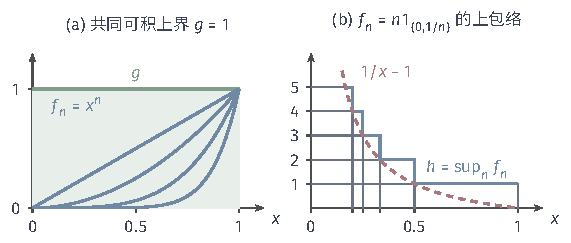
\includegraphics[width=96.633mm]{figures/02-abstract-mathematics/01-metric-and-measure/tikz/c3-dominating-envelope/figure.pdf}
 \caption{控制函数与上包络。(a)$[0,1]$上$f_n=x^n$（$n=1,2,4,8$）都位于可积函数$g=1$之下，积分$1/(n+1)\to0$。(b)$f_n=n\mathbf 1_{(0,1/n)}$（灰色，$n=1,\dots,5$）积分恒为$1$；上包络$h=\sup_nf_n$（蓝色阶梯）在$[\frac1{n+1},\frac1n)$上等于$n$，不小于$1/x-1$（红色虚线），后者在$(0,1)$上积分为$+\infty$，所以不存在可积的控制函数。}
 \label{fig:integ-dominating-envelope}
\end{figure}

支配条件是充分而非必要的：有些函数列没有可积的共同上界，积分仍然收敛。刻画积分收敛的确切条件需要一致可积性，它与依测度收敛等收敛方式一起在第~\ref{chap:normed-spaces}章讨论。在有限测度空间上，最常用的特例是：一致有界且几乎处处收敛的函数列，以常数为控制函数，积分可以与极限交换。

\section{累次积分}
\label{sec:integ-iterated}

计算平面区域上的累计时，我们习惯先沿一个方向积分，再沿另一个方向积分；计算双重级数时，先按行求和再把行和相加。这些做法都把一个联合累计拆成依次累计，并默认两种次序给出同一个结果。

有限矩阵的元素求和可以先行后列，也可以先列后行，这是有限加法的交换律。无穷的情形则需要条件，本节后面会给出一个无穷矩阵，两种次序的结果不同。下面先为两个测度空间的乘积建立集合族和乘积测度，再分别对非负函数与绝对可积函数证明这种拆分与换序成立。

\subsection{乘积测度}
\label{sec:integ-product-measure}

\paragraph{可测矩形与乘积$\sigma$代数}
设$(X,\mathcal A,\mu)$与$(Y,\mathcal B,\nu)$是测度空间。在$X\times Y$上，最简单的集合是$A\times B$，其中$A\in\mathcal A$、$B\in\mathcal B$，称为\term{可测矩形}（measurable rectangle）。它的“面积”应当是$\mu(A)\nu(B)$。可测矩形的有限并一般不再是矩形，所以要像上一章那样由它们生成$\sigma$代数。

\begin{definition}[乘积$\sigma$代数]
\label{def:integ-product-sigma}
由全体可测矩形生成的$\sigma$代数称为\term{乘积$\sigma$代数}（product sigma-algebra），记作$\mathcal A\otimes\mathcal B$。
\end{definition}

可测矩形的“边”可以是任意可测集，不必是区间。图~\ref{fig:integ-product-rectangles}(a)中$A$由两段组成，$A\times B$也就由两块组成，面积仍是$\lambda(A)\lambda(B)=1.8\times1=1.8$。

两个可测矩形之交仍是可测矩形：
\[
 (A\times B)\cap(A'\times B')=(A\cap A')\times(B\cap B').
\]
所以可测矩形构成$\pi$系统，后面的唯一性论证要用到这一点。

\begin{BookInlineFigure}
  \centering
  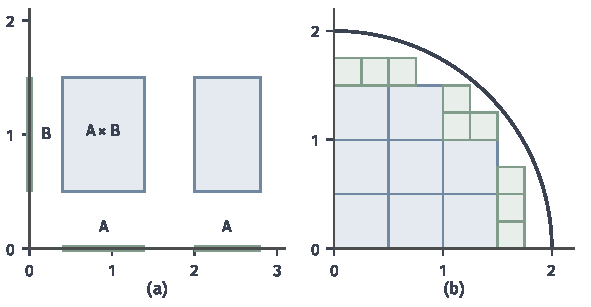
\includegraphics[width=100mm]{figures/04-spaces-measures-and-geometry/02-measure/matplotlib/integ-product-rectangles/figure.pdf}
  \caption{乘积可测结构由矩形生成。(a)取$A=[0.4,1.4]\cup[2.0,2.8]$、$B=[0.5,1.5]$，可测矩形$A\times B$由两块组成，绿色线段分别是$A$与$B$。(b)半径为$2$的四分之一圆盘不是矩形，蓝色矩形是边长$0.5$的网格中完全落在圆盘内的方格，绿色矩形是边长$0.25$的网格补充的方格；逐层加细的矩形不交并从内部逼近圆盘。}
  \label{fig:integ-product-rectangles}
\end{BookInlineFigure}

在欧氏空间上，乘积$\sigma$代数就是Borel代数：
\begin{equation}
 \mathcal B(\mathbb R)\otimes\mathcal B(\mathbb R)=\mathcal B(\mathbb R^2).
 \label{eq:integ-borel-product}
\end{equation}
一方面，开集是可数个有理顶点开矩形之并，开矩形是可测矩形，如图~\ref{fig:integ-product-rectangles}(b)所示，所以Borel集都在乘积$\sigma$代数中。另一方面，$A\times\mathbb R$是$A$在连续投影下的原像，对Borel集$A$是Borel集；$A\times B$是这样两个集合之交，也是Borel集。

\paragraph{截面}
依次累计的第一步是固定一个坐标。对$E\subseteq X\times Y$与$x\in X$，称$E_x=\{y\in Y:(x,y)\in E\}$为$E$在$x$处的\term{截面}（section）；类似地，$E^y=\{x\in X:(x,y)\in E\}$。对函数$f$，固定$x$得到截面函数$f_x(y)=f(x,y)$，固定$y$得到$f^y(x)=f(x,y)$。

截面的形状取决于固定哪个坐标。圆环在靠近中心的$x$处的截面是两段区间，在靠外的$x$处则是一段。下面先确认截面总是可测的，否则内层积分无从谈起。

\begin{lemma}[截面的可测性]
\label{lem:integ-section-measurable}
若$E\in\mathcal A\otimes\mathcal B$，则对每个$x$有$E_x\in\mathcal B$，对每个$y$有$E^y\in\mathcal A$。若$f$是$\mathcal A\otimes\mathcal B$可测函数，则每个$f_x$是$\mathcal B$可测的，每个$f^y$是$\mathcal A$可测的。
\end{lemma}

\begin{proof}
固定$x$，令$\mathcal E$为满足$E_x\in\mathcal B$的集合$E\subseteq X\times Y$全体。截面与补集、可数并可交换：
\[
 (X\times Y\setminus E)_x=Y\setminus E_x,\qquad\Bigl(\bigcup_nE_n\Bigr)_x=\bigcup_n(E_n)_x .
\]
所以$\mathcal E$是$\sigma$代数。对可测矩形，$(A\times B)_x$在$x\in A$时为$B$、否则为空集，所以$\mathcal E$含全部可测矩形，从而含$\mathcal A\otimes\mathcal B$。函数的情形由$\{f_x>a\}=(\{f>a\})_x$得到。$y$一侧对称。
\end{proof}

\paragraph{截面测度的可测性}
乘积测度的候选定义是沿$x$累计截面的测度，这相当于把区域切成薄片，每片的“长度”乘以厚度再相加：
\[
 E\mapsto\int_X\nu(E_x)\,\mathrm d\mu(x).
\]
为此要先知道$x\mapsto\nu(E_x)$可测。这一步需要$\sigma$有限条件。

\begin{lemma}[截面测度的可测性]
\label{lem:integ-section-measure}
设$\nu$是$\sigma$有限测度，$E\in\mathcal A\otimes\mathcal B$。则$x\mapsto\nu(E_x)$是$X$上的可测函数。
\end{lemma}

\begin{proof}
先设$\nu$有限。令$\mathcal D$为使$x\mapsto\nu(E_x)$可测的$E\in\mathcal A\otimes\mathcal B$全体。对可测矩形，$\nu((A\times B)_x)=\nu(B)\mathbf 1_A(x)$，可测，所以$\mathcal D$含可测矩形这一$\pi$系统。

$\mathcal D$是$\lambda$系统，逐条核对。全集$X\times Y$的截面测度是常数$\nu(Y)$。补集的截面测度为$\nu(Y)-\nu(E_x)$，这里用到$\nu$有限，差才有意义。不交可数并的截面测度是各截面测度之和，可测函数的可数和可测。由$\pi$--$\lambda$定理，$\mathcal D=\mathcal A\otimes\mathcal B$。

一般情形取$Y_m\in\mathcal B$两两不交、并为$Y$且$\nu(Y_m)<+\infty$，令$\nu_m(B)=\nu(B\cap Y_m)$。每个$\nu_m$有限，由上一段$x\mapsto\nu_m(E_x)$可测，而$\nu(E_x)=\sum_m\nu_m(E_x)$是可数个可测函数之和。
\end{proof}

\paragraph{乘积测度的构造}
截面测度可测以后，沿$x$累计截面测度就得到一个候选的乘积测度；沿$y$累计得到另一个候选。下面的定理说明二者是同一个测度，并且它由矩形上的取值唯一确定。

\begin{theorem}[乘积测度的存在唯一性]
\label{thm:integ-product-measure}
设$\mu,\nu$都是$\sigma$有限测度。则$\mathcal A\otimes\mathcal B$上存在唯一的测度$\pi$，使
\begin{equation}
 \pi(A\times B)=\mu(A)\nu(B),\qquad A\in\mathcal A,\ B\in\mathcal B,
 \label{eq:integ-product-rectangle}
\end{equation}
并且对每个$E\in\mathcal A\otimes\mathcal B$，
\begin{equation}
 \pi(E)=\int_X\nu(E_x)\,\mathrm d\mu(x)=\int_Y\mu(E^y)\,\mathrm d\nu(y).
 \label{eq:integ-product-sections}
\end{equation}
\end{theorem}

\begin{proof}
令$\pi_1(E)=\int_X\nu(E_x)\,\mathrm d\mu(x)$，由引理~\ref{lem:integ-section-measure}，被积函数非负可测。空集的截面都是空集，所以$\pi_1(\varnothing)=0$。若$E_n$两两不交，各截面$(E_n)_x$也两两不交，于是$\nu((\bigcup_nE_n)_x)=\sum_n\nu((E_n)_x)$。对$x$积分并用式~\eqref{eq:integ-series-termwise}逐项积分，得到
\[
 \pi_1\Bigl(\bigcup_nE_n\Bigr)=\sum_n\pi_1(E_n).
\]
所以$\pi_1$是测度。对矩形，
\[
 \pi_1(A\times B)=\int_X\nu(B)\mathbf 1_A\,\mathrm d\mu=\mu(A)\nu(B).
\]
同理$\pi_2(E)=\int_Y\mu(E^y)\,\mathrm d\nu(y)$也是满足式~\eqref{eq:integ-product-rectangle}的测度。

唯一性。取$X_n\in\mathcal A$、$Y_m\in\mathcal B$分别覆盖$X$、$Y$且测度有限，可数个矩形$X_n\times Y_m$覆盖$X\times Y$，在任何满足式~\eqref{eq:integ-product-rectangle}的测度下都取有限值。两个这样的测度在可测矩形这一$\pi$系统上相等，由第~\ref{chap:measure}章生成$\pi$系统上的唯一性定理，它们在$\mathcal A\otimes\mathcal B$上相等。特别地$\pi_1=\pi_2$，这就是式~\eqref{eq:integ-product-sections}。
\end{proof}

\begin{definition}[乘积测度]
\label{def:integ-product-measure}
定理~\ref{thm:integ-product-measure}中的测度称为$\mu$与$\nu$的\term{乘积测度}（product measure），记作$\mu\otimes\nu$。
\end{definition}

下面在一个可以逐项计算的网格上验证式~\eqref{eq:integ-product-sections}。两种切法分别相当于先按行、先按列累计，结果相同正是这个公式的含义。

\begin{example}[有限网格上的乘积测度]
\label{ex:integ-product-grid}
取$X=\{1,2\}$，质量为$\mu(\{1\})=1$、$\mu(\{2\})=2$；取$Y=\{a,b,c\}$，质量为$\nu(\{a\})=1$、$\nu(\{b\})=3$、$\nu(\{c\})=1$。乘积测度给格点$(i,y)$的质量$\mu(\{i\})\nu(\{y\})$。取
\[
 E=\{(1,a),(1,b),(2,b),(2,c)\}.
\]
按$x$切，两个截面的$\nu$测度为
\[
 \nu(E_1)=1+3=4,\qquad\nu(E_2)=3+1=4,
\]
于是
\[
 \int\nu(E_x)\,\mathrm d\mu=1\cdot4+2\cdot4=12 .
\]

按$y$切，三个截面的$\mu$测度为
\[
 \mu(E^a)=1,\qquad\mu(E^b)=1+2=3,\qquad\mu(E^c)=2,
\]
于是
\[
 \int\mu(E^y)\,\mathrm d\nu=1\cdot1+3\cdot3+1\cdot2=12 .
\]
两种切法得到同一个数。
\end{example}

\paragraph{与Lebesgue测度的关系}
在$\mathbb R^2$上，$\lambda\otimes\lambda$与第~\ref{chap:measure}章的二维Lebesgue测度$\lambda_2$都定义在式~\eqref{eq:integ-borel-product}的$\sigma$代数上，在左开右闭矩形上都等于边长之积；由唯一性它们相等。归纳可得$\lambda_d$等于$d$个$\lambda$的乘积。于是$\mathbb R^d$上Borel函数的积分可以逐个坐标计算，这是下面两个定理的主要用途。

\paragraph{乘积集合族与完备化}
乘积$\sigma$代数与测度的完备化是两回事。即使$\mu,\nu$都完备，$\mathcal A\otimes\mathcal B$也未必完备。取$\mathcal L$为Lebesgue可测集，$S\subseteq\mathbb R$不Lebesgue可测，$E=S\times\{0\}$。$E$含于$\mathbb R\times\{0\}$，后者的$\lambda\otimes\lambda$测度为$0$，所以$E$属于完备化；但截面$E^0=S$不可测，由引理~\ref{lem:integ-section-measurable}，$E\notin\mathcal L\otimes\mathcal L$。

二维Lebesgue可测集是$\lambda_2$的完备化，它比$\mathcal L\otimes\mathcal L$大。所以在完备化的乘积测度下，不能默认每个截面都可测；下面的定理会把这种例外限制在零测的参数集上。

\subsection{Tonelli定理}
\label{sec:integ-tonelli}

\paragraph{非负函数的换序}
式~\eqref{eq:integ-product-sections}说的是指示函数的联合积分等于两种次序的累次积分。对一般的非负函数，沿积分的构造步骤推广：指示函数、简单函数、递增极限。非负贡献不会相互抵消，所以结论允许各方都等于$+\infty$。先对一个变量积分、再对另一个变量积分所得的量称为\term{累次积分}（iterated integral）。

\begin{theorem}[Tonelli定理]
\label{thm:integ-tonelli}
设$\mu,\nu$都是$\sigma$有限测度，$f:X\times Y\to[0,+\infty]$是$\mathcal A\otimes\mathcal B$可测函数。则$x\mapsto\int_Yf_x\,\mathrm d\nu$与$y\mapsto\int_Xf^y\,\mathrm d\mu$分别可测，并且下面三者在$[0,+\infty]$中相等：
\begin{equation}
\begin{aligned}
 \int_{X\times Y}f\,\mathrm d(\mu\otimes\nu)&=\int_X\Bigl(\int_Yf(x,y)\,\mathrm d\nu(y)\Bigr)\mathrm d\mu(x)\\
 &=\int_Y\Bigl(\int_Xf(x,y)\,\mathrm d\mu(x)\Bigr)\mathrm d\nu(y).
\end{aligned}
 \label{eq:integ-tonelli}
\end{equation}
\end{theorem}

\begin{proof}
由引理~\ref{lem:integ-section-measurable}，各截面函数可测，内层积分有意义。证明按函数的构造分三步，只写$x$先固定的一侧，另一侧对称。

第一步，$f=\mathbf 1_E$，$E\in\mathcal A\otimes\mathcal B$。内层积分是$\nu(E_x)$，由引理~\ref{lem:integ-section-measure}可测，外层积分等于$(\mu\otimes\nu)(E)$，这就是式~\eqref{eq:integ-product-sections}。

第二步，$f$是非负简单函数，即有限个$c_i\mathbf 1_{E_i}$之和。内层积分是相应$c_i\nu((E_i)_x)$之和，可测，由线性性逐项得到式~\eqref{eq:integ-tonelli}。

第三步，一般的$f$。取二进分层逼近$\varphi_n\uparrow f$，每个$\varphi_n$是$\mathcal A\otimes\mathcal B$可测的简单函数。对每个$x$，$(\varphi_n)_x\uparrow f_x$，由单调收敛定理，
\[
 \int_Y(\varphi_n)_x\,\mathrm d\nu\uparrow\int_Yf_x\,\mathrm d\nu .
\]
作为可测函数的递增极限，$x\mapsto\int f_x\,\mathrm d\nu$可测。再对$x$用一次单调收敛定理，并在乘积空间上对$\varphi_n\uparrow f$用一次，由第二步的等式取极限即得。
\end{proof}

换序的实际用处是：内层积分按一种次序算不出来，换一种次序就能算。下面的例子中，$e^{y^2}$没有初等原函数，先对$y$积分行不通，先对$x$积分却只是乘以区间长度。

\begin{example}[换序计算]
\label{ex:integ-tonelli-swap}
计算累次积分
\[
 I=\int_0^1\Bigl(\int_x^1e^{y^2}\,\mathrm dy\Bigr)\mathrm dx .
\]
被积函数$f(x,y)=e^{y^2}\mathbf 1_{\{0\leq x\leq y\leq1\}}$非负且Borel可测，由Tonelli定理可以换序。固定$y$，$x$的截面是$[0,y]$，于是
\[
 I=\int_0^1\Bigl(\int_0^ye^{y^2}\,\mathrm dx\Bigr)\mathrm dy=\int_0^1ye^{y^2}\,\mathrm dy .
\]
令$w=y^2$，$\mathrm dw=2y\,\mathrm dy$，得到
\[
 I=\frac12\int_0^1e^w\,\mathrm dw=\frac{e-1}2 .
\]
换序之所以合法，只因为被积函数非负，不需要事先知道积分有限。
\end{example}

图~\ref{fig:integ-section-swap}画出了这个例子的积分区域。同一个三角形，竖着切时每个截面从对角线走到顶边，横着切时每个截面从左边走到对角线；换序就是把这两种切片方式互换，新的积分限要从图上读出来。

\begin{BookInlineFigure}
  \centering
  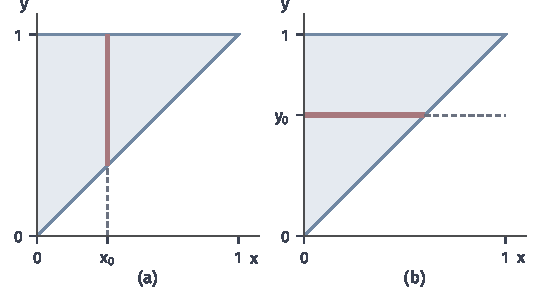
\includegraphics[width=92mm]{figures/04-spaces-measures-and-geometry/02-measure/matplotlib/integ-section-swap/figure.pdf}
  \caption{三角形$T=\{0\leq x\leq y\leq1\}$的两种截面。(a)固定$x=x_0$，红色线段是$y\in[x_0,1]$。(b)固定$y=y_0$，红色线段是$x\in[0,y_0]$，虚线部分不在$T$内。}
  \label{fig:integ-section-swap}
\end{BookInlineFigure}

\paragraph{完备化下的Tonelli定理}
若$f$只对完备化的乘积测度可测，截面函数可能不可测，结论要改成“几乎所有参数”。设$\mu,\nu$完备且$\sigma$有限，$f\geq0$对$\mu\otimes\nu$的完备化可测。

第一步找一个可测的替身。存在$\mathcal A\otimes\mathcal B$可测的$g\geq0$与$\mu\otimes\nu$零测集$N\in\mathcal A\otimes\mathcal B$，使$f=g$在$N$外成立：对指示函数，这就是完备化的定义（可测集等于乘积可测集并上零测集的子集），再经简单函数的递增逼近推广到一般的$f$。

第二步把零测的影响限制在参数上。由式~\eqref{eq:integ-product-sections}，$\int\nu(N_x)\,\mathrm d\mu=0$，所以对几乎每个$x$，$N_x$是$\nu$零测集。在这些$x$处，$f_x$与可测的$g_x$只在零测集上不同，由$\nu$的完备性可测，且积分相同。

对$g$用Tonelli定理，就得到式~\eqref{eq:integ-tonelli}，只是内层积分只对几乎每个$x$有定义，在例外的零测集上可以任意取值。$\mathbb R^d$上Lebesgue可测函数的累次积分正是这种情形。

\paragraph{$\sigma$有限条件}
$\sigma$有限条件不能省去。在$X=Y=[0,1]$上取$\mu$为Lebesgue测度，$\nu$为以全部Borel集为可测范围的计数测度，它不是$\sigma$有限的。对角线$D=\{(x,x):x\in[0,1]\}$是闭集，属于$\mathcal B([0,1])\otimes\mathcal B([0,1])$。

每个$x$截面$D_x=\{x\}$的计数为$1$，每个$y$截面$D^y=\{y\}$的Lebesgue测度为$0$，于是
\[
 \int_X\nu(D_x)\,\mathrm d\mu(x)=1,\qquad \int_Y\mu(D^y)\,\mathrm d\nu(y)=0 .
\]
两种次序不相等，式~\eqref{eq:integ-product-sections}失效。乘积测度构造中的唯一性论证正是在这里失去了依据：计数测度没有有限质量的覆盖片。

\paragraph{非负双重级数}
取两个$\mathbb N$上的计数测度，非负函数$a(m,n)=a_{m,n}$对乘积$\sigma$代数$\mathcal P(\mathbb N\times\mathbb N)$可测，乘积测度是$\mathbb N\times\mathbb N$上的计数测度。Tonelli定理给出
\[
 \sum_m\sum_na_{m,n}=\sum_n\sum_ma_{m,n},
\]
两边可以为$+\infty$：非负双重级数总可以交换求和次序。下一小节将看到，有正有负的双重级数并非如此。

\subsection{Fubini定理}
\label{sec:integ-fubini}

\paragraph{绝对可积函数的换序}
对取正负值或复值的函数，正负贡献的抵消可能依赖求和或积分的次序。解决办法是先对$\lvert f\rvert$用Tonelli定理核对绝对可积性，有了这一保证，再把$f$拆成正负部分或实部虚部，分别使用Tonelli定理。

\begin{theorem}[Fubini定理]
\label{thm:integ-fubini}
设$\mu,\nu$都是$\sigma$有限测度，$f$是$X\times Y$上$\mathcal A\otimes\mathcal B$可测的实值或复值函数，且
\begin{equation}
 \int_X\Bigl(\int_Y\lvert f(x,y)\rvert\,\mathrm d\nu(y)\Bigr)\mathrm d\mu(x)<+\infty .
 \label{eq:integ-fubini-condition}
\end{equation}
则$f$关于$\mu\otimes\nu$可积，并且：
\begin{enumerate}
 \item 对$\mu$-几乎每个$x$，$f_x$关于$\nu$可积；对$\nu$-几乎每个$y$，$f^y$关于$\mu$可积。
 \item 令$F(x)=\int_Yf_x\,\mathrm d\nu$，在$f_x$不可积的例外集上令$F(x)=0$，则$F$关于$\mu$可积；对$y$同样定义的$G$关于$\nu$可积。
 \item 三种累计相等：
 \begin{equation}
  \int_{X\times Y}f\,\mathrm d(\mu\otimes\nu)=\int_XF\,\mathrm d\mu=\int_YG\,\mathrm d\nu .
  \label{eq:integ-fubini}
 \end{equation}
\end{enumerate}
\end{theorem}

\begin{proof}
对$\lvert f\rvert$用Tonelli定理，式~\eqref{eq:integ-fubini-condition}的累次积分等于$\lvert f\rvert$在乘积空间上的积分，所以$f$可积。

令
\[
 N=\Bigl\{x:\ \int_Y\lvert f_x\rvert\,\mathrm d\nu=+\infty\Bigr\}.
\]
由Tonelli定理，它是可测集；又$x\mapsto\int\lvert f_x\rvert$的积分有限，由引理~\ref{lem:integ-null-sets}第2条，$\mu(N)=0$。这就是第1条。

先设$f$实值。$f^+$与$f^-$都是非负可测函数，由Tonelli定理，$x\mapsto\int f^\pm_x\,\mathrm d\nu$可测，积分分别等于$\int f^\pm\,\mathrm d(\mu\otimes\nu)$，都有限。在$N$外两者都有限，所以在$N$外有
\[
 F(x)=\int_Yf^+_x\,\mathrm d\nu-\int_Yf^-_x\,\mathrm d\nu .
\]
在$N$上$F=0$，所以$F$可测。对$F$积分，去掉零测集$N$不改变积分，得到
\[
\begin{aligned}
 \int_XF\,\mathrm d\mu&=\int_{X\setminus N}\Bigl(\int_Yf^+_x\,\mathrm d\nu\Bigr)\mathrm d\mu-\int_{X\setminus N}\Bigl(\int_Yf^-_x\,\mathrm d\nu\Bigr)\mathrm d\mu\\
 &=\int f^+\,\mathrm d(\mu\otimes\nu)-\int f^-\,\mathrm d(\mu\otimes\nu).
\end{aligned}
\]
右端就是$\int f\,\mathrm d(\mu\otimes\nu)$。$y$一侧对称。复值情形对实部与虚部分别使用实值结论，二者的例外集之并仍是零测集。
\end{proof}

截面只需几乎处处可积，这是由内层积分自身的性质决定的：对某个零测的$x$集合，$f_x$可能不可积，内层积分没有定义。把这些点上的$F$统一取零，得到的是一个可测的外层被积函数，而外层积分看不见零测集上的取值。若改用完备化的乘积测度，再结合上一小节的完备化讨论，结论同样成立，只是截面可测性本身也只对几乎每个参数成立。

\paragraph{缺少绝对可积时的反例}
绝对可积的假设不能去掉。考虑$\mathbb N\times\mathbb N$上的计数测度与下面的无穷矩阵，图~\ref{fig:integ-fubini-counterexample}画出了它的左上角：
\[
 a_{i,j}=\begin{cases}1,&j=i,\\-1,&j=i+1,\\0,&\text{其他}.\end{cases}
\]

先按行累计。每一行只有$+1$与$-1$两个非零元，行和为$0$，所以
\[
 \sum_i\sum_ja_{i,j}=0 .
\]
再按列累计。第一列只有$a_{1,1}=1$，列和为$1$；第$j\geq2$列有$a_{j,j}=1$与$a_{j-1,j}=-1$，列和为$0$，所以
\[
 \sum_j\sum_ia_{i,j}=1 .
\]

\begin{BookInlineFigure}
  \centering
  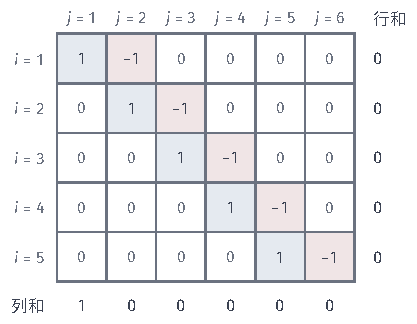
\includegraphics[width=70.672mm]{figures/04-spaces-measures-and-geometry/02-measure/tikz/integ-fubini-counterexample/figure.pdf}
  \caption{无穷矩阵$a_{i,j}$的左上角五行六列，矩阵向右下方继续。蓝色单元为$+1$，红色单元为$-1$。右侧是整行的和，下方是整列的和；第六列的$+1$位于第六行，在图外。}
  \label{fig:integ-fubini-counterexample}
\end{BookInlineFigure}

两种次序给出不同结果。原因是$\sum_{i,j}\lvert a_{i,j}\rvert=+\infty$，Fubini定理的条件不成立；每一行、每一列单独看都绝对可和，这并不够。这与有限矩阵不同：有限矩阵的两种次序总相同，因为有限和的重排不需要任何条件。

使用Fubini定理的标准步骤因此是：先对$\lvert f\rvert$任选一种方便的次序作累次积分，由Tonelli定理确认结果有限；然后才可以对$f$本身任意换序。对有界函数和有限测度，例如有界区域上的有界可测函数，第一步自动成立。

\section{微积分基本定理}
\label{sec:integ-ftc}

卷一的微积分基本定理有两个方向。被积函数$g$连续时，累计函数$G(x)=\int_a^xg(t)\,\mathrm dt$可导且$G'=g$；$F$连续可导时，$F(b)-F(a)=\int_a^bF'(t)\,\mathrm dt$。

有了Lebesgue积分，被积函数只需可积，导数也只需几乎处处存在，两个方向都要重新回答：可积函数的累计函数在什么意义下可导，导数是否回到被积函数？哪些函数能由几乎处处导数的积分恢复？本节在有界闭区间$[a,b]$上回答这两个问题，测度都是Lebesgue测度。

\subsection{变上限积分的导数}
\label{sec:integ-indefinite-derivative}

\paragraph{绝对连续函数}
先看什么样的函数有希望写成某个函数的累计。一致连续要求：区间足够短时，函数在两端的增量就小。要由导数恢复增量，这还不够。导数为零的点之间可能散布着许多极短的区间，函数恰好在这些区间上完成全部增长。需要控制的是许多互不相交的小区间上的\emph{总}增量。

\begin{definition}[绝对连续函数]
\label{def:integ-absolutely-continuous}
设$F:[a,b]\to\mathbb R$。若对任意$\varepsilon>0$存在$\delta>0$，使对$[a,b]$中任意有限个两两不交的开区间$(a_i,b_i)$（$i=1,\dots,m$），只要总长满足
\begin{equation}
 \sum_{i=1}^m(b_i-a_i)<\delta,
 \label{eq:integ-ac-length}
\end{equation}
就有
\begin{equation}
 \sum_{i=1}^m\lvert F(b_i)-F(a_i)\rvert<\varepsilon,
 \label{eq:integ-ac-increment}
\end{equation}
则称$F$为$[a,b]$上的\term{绝对连续函数}（absolutely continuous function）。
\end{definition}

取$m=1$就回到一致连续，所以绝对连续函数一致连续。区别在于$\delta$必须对任意多个小区间同时有效：区间个数不受限制，只限制总长度。图~\ref{fig:integ-absolute-continuity-intervals}中$F(x)=\sqrt x$，四段绿色区间总长$1.2$，对应的增量为
\[
 0.260,\qquad0.158,\qquad0.090,\qquad0.053,
\]
和约为$0.562$。绝对连续性要求，当总长趋于零时，增量之和也一致地趋于零，无论区间怎样分布、分成多少段。

\begin{BookInlineFigure}
  \centering
  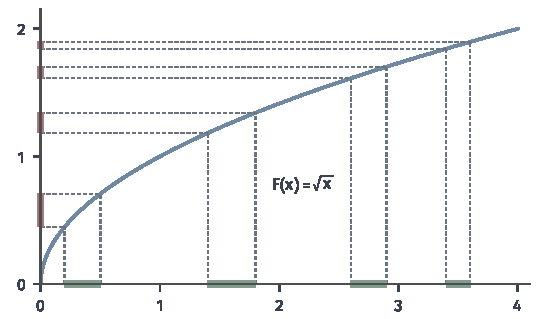
\includegraphics[width=92mm]{figures/04-spaces-measures-and-geometry/02-measure/matplotlib/integ-absolute-continuity-intervals/figure.pdf}
  \caption{绝对连续性控制的是多个不交区间上的总增量。$F(x)=\sqrt x$（蓝）。横轴上的绿色区间为$(0.2,0.5)$、$(1.4,1.8)$、$(2.6,2.9)$、$(3.4,3.6)$，纵轴上的红色线段是相应增量。靠近原点的区间虽短，增量却最大。}
  \label{fig:integ-absolute-continuity-intervals}
\end{BookInlineFigure}

若$F$满足Lipschitz条件$\lvert F(x)-F(y)\rvert\leq L\lvert x-y\rvert$，则总增量不超过$L$乘以总长度，取$\delta=\varepsilon/L$即可，所以Lipschitz函数绝对连续。$[a,b]$上连续可导的函数由中值定理满足Lipschitz条件，因而绝对连续。有限线性组合保持绝对连续，由三角不等式对各函数分别取$\delta$再取最小值即得。

这里的“绝对连续”描述函数增量受区间长度控制，与第~\ref{chap:measure-densities}章两个测度之间的绝对连续是不同的定义，两者的联系在那里说明。

\paragraph{变上限积分的绝对连续性}
设$g$在$[a,b]$上可积，令
\begin{equation}
 G(x)=\int_a^xg(t)\,\mathrm dt,\qquad a\leq x\leq b,
 \label{eq:integ-indefinite}
\end{equation}
称为$g$的\term{变上限积分}（indefinite integral）。多个不交区间上$G$的增量之和不超过$\lvert g\rvert$在这些区间之并上的积分，所以要证$G$绝对连续，需要的是：测度很小的集合上，$\lvert g\rvert$的积分也很小。

\begin{lemma}[积分的绝对连续性]
\label{lem:integ-small-sets}
设$g$关于$\mu$可积。则对任意$\varepsilon>0$存在$\delta>0$，使对每个满足$\mu(A)<\delta$的可测集$A$，都有$\int_A\lvert g\rvert\,\mathrm d\mu<\varepsilon$。
\end{lemma}

\begin{proof}
把$\lvert g\rvert$分成有界的截断$\min\{\lvert g\rvert,n\}$与尾部。截断随$n$递增到$\lvert g\rvert$，由单调收敛定理，$\int\min\{\lvert g\rvert,n\}\uparrow\int\lvert g\rvert<+\infty$。所以可取$n$使尾部满足
\[
 \int\bigl(\lvert g\rvert-\min\{\lvert g\rvert,n\}\bigr)\,\mathrm d\mu<\frac\varepsilon2 .
\]
令$\delta=\varepsilon/(2n)$。当$\mu(A)<\delta$时，截断部分不超过高度$n$乘以测度，于是
\[
 \int_A\lvert g\rvert\,\mathrm d\mu\leq\int_A\min\{\lvert g\rvert,n\}\,\mathrm d\mu+\frac\varepsilon2<n\delta+\frac\varepsilon2=\varepsilon .
\]
\end{proof}

对$[a,b]$中两两不交的$(a_i,b_i)$，令$A=\bigcup_i(a_i,b_i)$，由绝对值估计，
\[
 \sum_i\lvert G(b_i)-G(a_i)\rvert=\sum_i\Bigl\lvert\int_{a_i}^{b_i}g\Bigr\rvert\leq\int_A\lvert g\rvert\,\mathrm d\lambda .
\]
总长$\lambda(A)<\delta$时右侧小于$\varepsilon$，所以$G$绝对连续。例如在$[0,4]$上取$g(t)=1/(2\sqrt t)$，它在原点附近无界，但由反常积分定理$\int_0^xg=\sqrt x$，所以$\sqrt x$绝对连续；它在原点附近斜率无界，不是Lipschitz函数。

这里要区分两种对象。$g$只确定到零测集：在零测集上改动$g$，$G$完全不变。$G$却在每个点都有确定的值，并且是连续函数。所以下面关于$G'$的结论只能是“几乎处处等于$g$”，不能期望在每一点成立。

\paragraph{Vitali覆盖}
要研究$G'$，先要知道单调函数几乎处处可导，证明的核心是一个区间选择引理。设想要用彼此不重叠的短区间尽量铺满一个集合，手边有很多候选区间，每个点附近都有任意短的候选。

设$E\subseteq\mathbb R$，$\mathcal V$是一族非退化闭区间；若对每个$x\in E$和每个$\eta>0$，都有$I\in\mathcal V$满足$x\in I$且长度$\lvert I\rvert<\eta$，称$\mathcal V$为$E$的\term{Vitali覆盖}（Vitali cover）。

\begin{lemma}[Vitali覆盖引理]
\label{lem:integ-vitali}
设$E\subseteq\mathbb R$的外测度$\lambda^*(E)<\infty$，$\mathcal V$是$E$的Vitali覆盖。则对任意$\varepsilon>0$，存在$\mathcal V$中有限个两两不交的区间$I_1,\dots,I_N$，使
\begin{equation}
 \lambda^*\Bigl(E\setminus\bigcup_{k=1}^NI_k\Bigr)<\varepsilon .
 \label{eq:integ-vitali}
\end{equation}
\end{lemma}

\begin{proof}
取开集$O\supseteq E$，$\lambda(O)<\infty$，只保留$\mathcal V$中含于$O$的区间；$O$是开集，每点附近足够短的区间都含于$O$，所以剩下的仍是Vitali覆盖。

归纳地选取区间，每次都选得尽量长。设已选出两两不交的$I_1,\dots,I_n$。若它们已覆盖$E$，结论成立。否则令$k_n$为$\mathcal V$中与$I_1,\dots,I_n$都不相交的区间长度的上确界。$E$中未被覆盖的点到闭集$I_1\cup\dots\cup I_n$有正距离，所以$0<k_n\leq\lambda(O)$。选取与已选区间不交的$I_{n+1}\in\mathcal V$，使$\lvert I_{n+1}\rvert>k_n/2$。

所选区间两两不交，含于$O$，故$\sum_n\lvert I_n\rvert\leq\lambda(O)<\infty$。于是长度趋于零，并且
\[
 k_n<2\lvert I_{n+1}\rvert\to0 .
\]

取$N$使$\sum_{n>N}\lvert I_n\rvert<\varepsilon/5$，记$5I_n$为与$I_n$同心、长度为$5\lvert I_n\rvert$的闭区间。任取$x\in E\setminus\bigcup_{k\leq N}I_k$，存在$I\in\mathcal V$含$x$且与$I_1,\dots,I_N$都不相交。$I$不能与全部$I_n$都不相交，否则$\lvert I\rvert\leq k_n\to0$，与$I$非退化矛盾。

设$n$是使$I\cap I_n\neq\varnothing$的最小下标，则$n>N$，并且$I$与前$n-1$个区间都不相交，所以$\lvert I\rvert\leq k_{n-1}<2\lvert I_n\rvert$。于是$x$到$I_n$中点的距离满足
\[
 \mathrm{dist}\leq\lvert I\rvert+\tfrac12\lvert I_n\rvert<\tfrac52\lvert I_n\rvert,
\]
即$x\in5I_n$。未覆盖部分含于$\bigcup_{n>N}5I_n$，外测度小于$\varepsilon$。
\end{proof}

图~\ref{fig:integ-vitali-cover}展示了最后一步的放大论证：未选中的区间$I$若碰到某个已选区间$I_n$，且长度不超过$I_n$的两倍，就整个落在$5I_n$之内。已选区间的五倍放大接住了所有漏掉的点，而尾部区间的总长任意小。

\begin{BookInlineFigure}
  \centering
  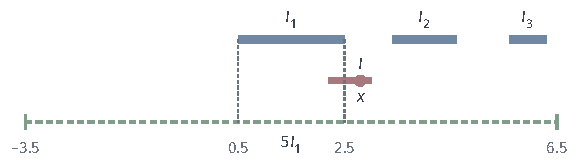
\includegraphics[width=97.991mm]{figures/04-spaces-measures-and-geometry/02-measure/tikz/integ-vitali-cover/figure.pdf}
  \caption{Vitali选择中的五倍放大。蓝色为已选的两两不交区间$I_1=[0.5,2.5]$、$I_2=[3.4,4.6]$、$I_3=[5.6,6.3]$；红色区间$I=[2.2,3.0]$含点$x$，与$I_1$相交且$\lvert I\rvert=0.8<2\lvert I_1\rvert$，因此落在与$I_1$同心、长为$10$的区间$5I_1=[-3.5,6.5]$（绿色虚线）中。}
  \label{fig:integ-vitali-cover}
\end{BookInlineFigure}

\paragraph{单调函数的导数}
为描述导数可能不存在的情况，对$x\in(a,b)$引入右侧差商$\bigl(F(x+h)-F(x)\bigr)/h$在$h\downarrow0$时的上极限$D^+F(x)$与下极限$D_+F(x)$，以及左侧差商$\bigl(F(x)-F(x-h)\bigr)/h$的上极限$D^-F(x)$与下极限$D_-F(x)$，统称\term{Dini导数}（Dini derivative）。$F$在$x$处可导当且仅当四者相等且有限。

下面的证明还要用到积分的平移不变性：对可积或非负可测的$\phi$与实数$h$，有
\[
 \int_{[a,b]}\phi(x+h)\,\mathrm dx=\int_{[a+h,b+h]}\phi(x)\,\mathrm dx .
\]
对指示函数这就是Lebesgue测度的平移不变性，由线性性推广到简单函数，再由递增逼近推广到非负可测函数和可积函数。

单调函数的增量总和被端点差控制，这个全局约束足以迫使差商在几乎每一点收敛。

\begin{theorem}[单调函数几乎处处可导]
\label{thm:integ-monotone-differentiable}
设$F:[a,b]\to\mathbb R$单调不减。则$F$在$[a,b]$上几乎处处有有限导数，$F'$（在导数不存在处取$0$）可积，并且
\begin{equation}
 \int_a^bF'(x)\,\mathrm dx\leq F(b)-F(a).
 \label{eq:integ-monotone-derivative-bound}
\end{equation}
\end{theorem}

\begin{proof}
先证四个Dini导数几乎处处相等。取有理数$0<u<v$，令
\[
 E=\{x\in(a,b):D_-F(x)<u<v<D^+F(x)\},\qquad s=\lambda^*(E).
\]
思路是用$E$上的两种差商夹出矛盾：左侧小区间上增量小于$u$倍长度，右侧小区间上增量大于$v$倍长度。

对$\varepsilon>0$取开集$O\supseteq E$，$\lambda(O)<s+\varepsilon$。每个$x\in E$都有任意小的$h>0$，使$[x-h,x]\subseteq O\cap(a,b)$且$F(x)-F(x-h)<uh$。这些区间构成$E$的Vitali覆盖，由引理~\ref{lem:integ-vitali}选出两两不交的$[x_k-h_k,x_k]$（$k\leq N$），未覆盖部分外测度小于$\varepsilon$，并且
\[
 \sum_k\bigl(F(x_k)-F(x_k-h_k)\bigr)<u\lambda(O)<u(s+\varepsilon).
\]

令$A$为$E$落在这些区间内部的部分，则$\lambda^*(A)>s-\varepsilon$。每个$y\in A$都有任意小的$k>0$，使$[y,y+k]$含于某个$(x_j-h_j,x_j)$且$F(y+k)-F(y)>vk$。再用引理选出两两不交的$J_1,\dots,J_M$，总长大于$s-2\varepsilon$，于是$F$在这些区间上的增量之和大于$v(s-2\varepsilon)$。

$F$单调不减，同一个$[x_k-h_k,x_k]$内不交子区间上的增量之和不超过它两端的增量。比较两次估计，得到
\[
 v(s-2\varepsilon)<u(s+\varepsilon).
\]
令$\varepsilon\to0$得$vs\leq us$。由$u<v$，只能$s=0$。

对所有有理数对取并，$D^+F\leq D_-F$几乎处处成立。把这一结论用于单调不减函数$\tilde F(x)=-F(-x)$，得到$D^-F\leq D_+F$几乎处处成立。于是几乎处处有
\[
 D^+F\leq D_-F\leq D^-F\leq D_+F\leq D^+F .
\]
四者相等，导数在$[0,+\infty]$中几乎处处存在。

再证积分估计，它同时说明导数几乎处处有限。对$x>b$令$F(x)=F(b)$，令$q_n(x)=n\bigl(F(x+1/n)-F(x)\bigr)$。单调函数的阈值集合是区间，所以$q_n$是非负可测函数，并在导数存在处$q_n\to F'$。由Fatou引理与平移不变性，
\[
\begin{aligned}
 \int_a^bF'\,\mathrm dx&\leq\liminf_n\int_a^bq_n\,\mathrm dx\\
 &=\liminf_n\Bigl(n\int_b^{b+1/n}F\,\mathrm dx-n\int_a^{a+1/n}F\,\mathrm dx\Bigr).
\end{aligned}
\]
在$[b,b+1/n]$上$F=F(b)$，在$[a,a+1/n]$上$F\geq F(a)$，所以右端不超过$F(b)-F(a)$。左侧有限，非负可积函数几乎处处有限。
\end{proof}

式~\eqref{eq:integ-monotone-derivative-bound}只是不等式。$[0,1]$上的阶跃函数$\mathbf 1_{[1/2,1]}$单调不减，除$x=1/2$外导数都是$0$，导数的积分为$0$，而端点增量为$1$；增量全部发生在一个点上，导数读不到它。所以单调性只给出导数的存在与总量的上界。

\paragraph{变上限积分的导数}
现在回到$G(x)=\int_a^xg$。证明思路是先得到$\int_a^c(G'-g)=0$对每个$c$成立，所以需要一个判零引理：区间上的积分全为零的函数几乎处处为零。

\begin{lemma}[区间积分全为零的函数]
\label{lem:integ-vanishing-intervals}
设$g$在$[a,b]$上可积且为实值。若对每个$x\in[a,b]$都有$\int_a^xg=0$，则$g=0$几乎处处成立。
\end{lemma}

\begin{proof}
Lebesgue可测函数与某个Borel函数几乎处处相等，改动零测集不影响结论，不妨设$g$是Borel函数。令$\mathcal D$为使$\int_Eg=0$的Borel集$E\subseteq[a,b]$全体。

区间$(c,d]\subseteq[a,b]$满足
\[
 \int_{(c,d]}g=\int_a^dg-\int_a^cg=0,
\]
这些区间与空集对有限交封闭，并生成$[a,b]$上的Borel集（单点零测，可以并入）。

$\mathcal D$是$\lambda$系统：$[a,b]\in\mathcal D$；补集由$\int_{E^c}g=\int g-\int_Eg$得到；两两不交的可数并由支配收敛（以$\lvert g\rvert$为控制）得到。由$\pi$--$\lambda$定理，$\mathcal D$包含全部Borel集。取$E=\{g>0\}$，得$\int g^+=0$，所以$g\leq0$几乎处处成立；同理$g\geq0$几乎处处成立。
\end{proof}

现在可以陈述本小节的主要结论。

\begin{theorem}[Lebesgue微分定理]
\label{thm:integ-lebesgue-differentiation}
设$g$在$[a,b]$上可积，$G$由式~\eqref{eq:integ-indefinite}给出。则$G$绝对连续，$G$几乎处处可导，并且$G'=g$几乎处处成立，即对几乎每个$x\in(a,b)$，
\begin{equation}
 \lim_{h\to0}\frac1h\int_x^{x+h}g(t)\,\mathrm dt=g(x).
 \label{eq:integ-lebesgue-differentiation}
\end{equation}
其中$h<0$时$\int_x^{x+h}$理解为$-\int_{x+h}^x$。
\end{theorem}

\begin{proof}
绝对连续性已经证明。复值情形对实部、虚部分别处理；实值情形由$g=g^+-g^-$与导数的线性性，只需对$g\geq0$证明。

先设$0\leq g\leq M$。此时$G$单调不减且是Lipschitz函数，由定理~\ref{thm:integ-monotone-differentiable}几乎处处可导。对$x>b$令$G(x)=G(b)$，差商$q_n(x)=n\bigl(G(x+1/n)-G(x)\bigr)$满足$0\leq q_n\leq M$，并在$G$可导处趋于$G'$。对$c\in(a,b]$，在$[a,c]$上以常数$M$为控制用支配收敛，再平移，得
\[
 \int_a^cG'\,\mathrm dx=\lim_{n\to\infty}\Bigl(n\int_c^{c+1/n}G\,\mathrm dx-n\int_a^{a+1/n}G\,\mathrm dx\Bigr).
\]
$G$连续，函数在缩小区间上的平均值趋于端点值，所以右端等于$G(c)-G(a)$。于是
\[
 \int_a^c(G'-g)\,\mathrm dx=0
\]
对所有$c$成立，由引理~\ref{lem:integ-vanishing-intervals}，$G'=g$几乎处处成立。

再看一般的$g\geq0$。令$g_n=\min\{g,n\}$，$G_n(x)=\int_a^xg_n$。由有界情形，$G_n'=g_n$几乎处处成立。函数$G-G_n=\int_a^x(g-g_n)$单调不减，其导数几乎处处非负，所以$G'\geq g_n$几乎处处成立；合并可数个例外集，得$G'\geq g$几乎处处成立。

另一方面，由式~\eqref{eq:integ-monotone-derivative-bound}，
\[
 \int_a^bG'\,\mathrm dx\leq G(b)-G(a)=\int_a^bg\,\mathrm dx .
\]
因此$G'-g\geq0$几乎处处成立且积分不超过$0$，由定理~\ref{thm:integ-monotonicity}，$G'=g$几乎处处成立。
\end{proof}

定理的名称来自式~\eqref{eq:integ-lebesgue-differentiation}：$g$在$x$附近的局部平均值，在几乎每一点恢复$g$的取值。卷一要求$g$连续，结论在每一点成立；这里$g$只是可积，结论在零测集外成立。

下面用一个能手算的例子看例外集。在$[0,2]$上取$g=\mathbf 1_{[0,1]}$，变上限积分是
\[
 G(x)=\min\{x,1\}.
\]
除$x=1$外$G$都可导，$x<1$时$G'=1=g$，$x>1$时$G'=0=g$；在$x=1$处$G$有折角，导数不存在。例外集是单点，与定理相符。

$[0,1]$上的$\mathbf 1_{\mathbb Q}$说明“几乎处处”不能改成“处处”：它的变上限积分恒为$0$，导数$0$与$\mathbf 1_{\mathbb Q}$在每个有理点都不同。

\subsection{由导数恢复函数}
\label{sec:integ-recovery}

\paragraph{有界变差与导数的存在}
现在处理第二个方向：给定绝对连续的$F$，要证明$F(x)=F(a)+\int_a^xF'$。第一步是确认$F'$几乎处处存在且可积。对$[a,b]$的分割$P:a=x_0<\dots<x_n=b$，令
\[
 V(F,P)=\sum_k\lvert F(x_k)-F(x_{k-1})\rvert .
\]
称$V_a^b(F)=\sup_PV(F,P)$为$F$在$[a,b]$上的变差，它是函数图像沿纵向走过的总路程；若它有限，称$F$为\term{有界变差函数}（function of bounded variation）。在分割中插入点只会使$V(F,P)$不减，所以变差对区间可加：$V_a^b(F)=V_a^c(F)+V_c^b(F)$。

\begin{lemma}[绝对连续函数有界变差]
\label{lem:integ-ac-bv}
若$F$在$[a,b]$上绝对连续，则$F$是有界变差函数，并且是两个单调不减函数之差。
\end{lemma}

\begin{proof}
对$\varepsilon=1$取定义中的$\delta$，把$[a,b]$等分成$K$段，每段长度小于$\delta$。在一段$[c,d]$内任取分割，其小区间两两不交、总长小于$\delta$，增量之和小于$1$，故$V_c^d(F)\leq1$。由区间可加性，$V_a^b(F)\leq K$。

令$V(x)=V_a^x(F)$。对$x<y$，$V(y)-V(x)=V_x^y(F)\geq\lvert F(y)-F(x)\rvert$，所以$V$与$V-F$都单调不减，而$F=V-(V-F)$。
\end{proof}

由定理~\ref{thm:integ-monotone-differentiable}，两个单调函数都几乎处处可导且导数可积，所以绝对连续函数$F$几乎处处可导，$F'$可积。

\paragraph{零导数引理}
令$H(x)=F(x)-F(a)-\int_a^xF'$。由上一小节，$H$绝对连续且$H'=F'-F'=0$几乎处处成立。恢复公式就归结为：导数几乎处处为零的绝对连续函数必为常数。阶跃函数说明没有绝对连续性时这不成立；绝对连续性的作用，是控制导数为零的点之外那些总长很小的间隙上的增量。

\begin{lemma}[零导数引理]
\label{lem:integ-zero-derivative}
若$H$在$[a,b]$上绝对连续，且$H'=0$几乎处处成立，则$H$是常数。
\end{lemma}

\begin{proof}
任取$c\in(a,b]$，证明$H(c)=H(a)$。给定$\varepsilon>0$，取绝对连续定义中的$\delta$。令$E=\{x\in(a,c):H'(x)=0\}$，则$\lambda(E)=c-a$。

对每个$x\in E$，有任意小的$h>0$使$[x,x+h]\subseteq(a,c)$且$\lvert H(x+h)-H(x)\rvert<\varepsilon h$。这些区间构成$E$的Vitali覆盖，由引理~\ref{lem:integ-vitali}选出两两不交的$[x_k,y_k]$（$k=1,\dots,N$，按$x_1<y_1<x_2<\dots<y_N$排列），使$\lambda\bigl(E\setminus\bigcup_k[x_k,y_k]\bigr)<\delta$。

记$y_0=a$、$x_{N+1}=c$。剩下的间隙$(y_k,x_{k+1})$两两不交，总长小于$\delta$。把端点增量沿选中区间和间隙拆开：
\[
 \lvert H(c)-H(a)\rvert\leq\sum_{k=1}^N\lvert H(y_k)-H(x_k)\rvert+\sum_{k=0}^N\lvert H(x_{k+1})-H(y_k)\rvert .
\]
第一个和由导数为零控制，不超过$\varepsilon\sum_k(y_k-x_k)\leq\varepsilon(c-a)$；第二个和由绝对连续性控制，小于$\varepsilon$。于是
\[
 \lvert H(c)-H(a)\rvert<\varepsilon(c-a)+\varepsilon .
\]
$\varepsilon$任意，所以$H(c)=H(a)$。
\end{proof}

\paragraph{恢复公式}
零导数引理补上了最后一步，两个方向合起来给出一个双向刻画。

\begin{theorem}[Lebesgue微积分基本定理]
\label{thm:integ-ftc}
设$F:[a,b]\to\mathbb R$。以下两条等价：
\begin{enumerate}
 \item $F$在$[a,b]$上绝对连续；
 \item 存在$[a,b]$上的可积函数$g$，使$F(x)=F(a)+\int_a^xg(t)\,\mathrm dt$对所有$x\in[a,b]$成立。
\end{enumerate}
此时$F$几乎处处可导，$F'=g$几乎处处成立，并且对任意$c,x\in[a,b]$，
\begin{equation}
 F(x)=F(c)+\int_c^xF'(t)\,\mathrm dt,
 \label{eq:integ-ftc}
\end{equation}
其中$x<c$时$\int_c^x$理解为$-\int_x^c$。
\end{theorem}

\begin{proof}
(2)推出(1)及$F'=g$几乎处处成立，就是定理~\ref{thm:integ-lebesgue-differentiation}。

(1)推出(2)。由引理~\ref{lem:integ-ac-bv}，$F'$几乎处处存在且可积。令$H(x)=F(x)-F(a)-\int_a^xF'$，它绝对连续且$H'=0$几乎处处成立。由引理~\ref{lem:integ-zero-derivative}，$H\equiv H(a)=0$，取$g=F'$即得(2)。

式~\eqref{eq:integ-ftc}由$x$与$c$两处的(2)相减得到。
\end{proof}

这一形式的\term{微积分基本定理}（fundamental theorem of calculus）说：绝对连续函数恰好是可积函数的变上限积分加上常数，这个可积函数在几乎处处的意义下唯一确定为$F'$。

式~\eqref{eq:integ-ftc}说明怎样恢复整个函数：只需知道一点的函数值$F(c)$和一个可积的导数代表。导数在零测集上的取值无关紧要，函数值却要在一点给定，否则只能恢复到相差一个常数。

例如$F(x)=\lvert x\rvert$在$[-1,1]$上是Lipschitz函数，因而绝对连续。除$x=0$外$F'(x)=\operatorname{sgn}x$。从$c=-1$出发恢复，
\[
 F(0)=F(-1)+\int_{-1}^0(-1)\,\mathrm dt=1-1=0,
\]
再继续恢复到右端点，
\[
 F(1)=F(0)+\int_0^11\,\mathrm dt=1 .
\]
两个值都与$\lvert x\rvert$一致；$F'$在$x=0$处没有定义，并不影响恢复。

\paragraph{Cantor函数}
仅有连续性和几乎处处可导，还不能保证恢复公式。下面用Cantor集构造一个反例。记第~\ref{chap:measure}章Cantor集构造中第$n$步的$2^n$个保留闭区间之并为$C_n$。令$c_n:[0,1]\to[0,1]$是这样的连续分段线性函数：$c_n(0)=0$，在$C_n$的每个保留区间上线性增加$2^{-n}$，在已删去的开区间上取常值，于是$c_n(1)=1$。

从$c_n$到$c_{n+1}$，在每个保留区间上，原来线性增加的$2^{-n}$被分成左、右三分之一上各增加$2^{-n-1}$，中间三分之一上不变；两端的值不变。在同一个保留区间上，$c_n$与$c_{n+1}$都是单调函数，从相同的起点走到相同的终点，总上升量是$2^{-n}$，所以二者之差不超过$2^{-n}$。在已删去的区间上二者相等。于是
\[
 \sup_{[0,1]}\lvert c_{n+1}-c_n\rvert\leq2^{-n}.
\]
所以$c_n$一致收敛到一个连续函数$c$，称为\term{Cantor函数}（Cantor function）。它单调不减，$c(0)=0$，$c(1)=1$，并且在每个删去的开区间上取常值，因为从删去这一区间的那一步起，所有$c_n$在其上都取同一个常值。图~\ref{fig:integ-cantor-function}画出了前几步的逼近。

\begin{BookInlineFigure}
  \centering
  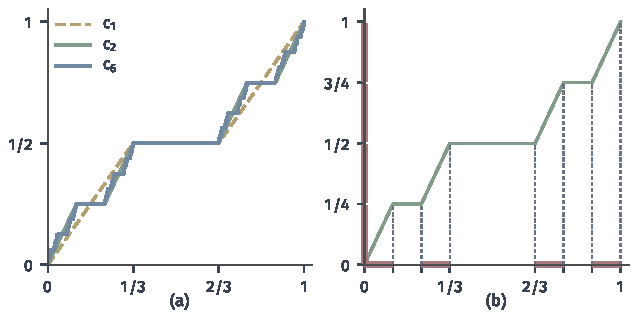
\includegraphics[width=108mm]{figures/04-spaces-measures-and-geometry/02-measure/matplotlib/integ-cantor-function/figure.pdf}
  \caption{Cantor函数及其分段线性逼近。(a)$c_1$（黄色虚线）、$c_2$（绿）与$c_6$（蓝），$c_n$在第$n$步的$2^n$个保留区间上线性增加$2^{-n}$，在已删去的区间上保持常值。(b)第二步的四个保留区间$[0,\frac19]$、$[\frac29,\frac13]$、$[\frac23,\frac79]$、$[\frac89,1]$（横轴红色）总长$\frac49$，对应的增量（纵轴红色）各为$\frac14$，合起来覆盖整个$[0,1]$。}
  \label{fig:integ-cantor-function}
\end{BookInlineFigure}

$[0,1]\setminus C$是删去的开区间之并，$c$在其中每一点导数为$0$；$\lambda(C)=0$，所以$c'=0$几乎处处成立，而
\[
 \int_0^1c'(x)\,\mathrm dx=0\neq1=c(1)-c(0).
\]
恢复公式失败，由定理~\ref{thm:integ-ftc}，$c$不绝对连续。这也可以直接从定义看出：第$n$步的$2^n$个保留区间（取其内部）两两不交，总长$(2/3)^n\to0$，$c$在它们上的增量之和始终是$1$。

Cantor函数把几种容易混淆的性质分开了。它连续，所以连续不能保证恢复公式；它单调，因而有界变差并且几乎处处可导，所以这两条也不够；它缺的正是绝对连续性。在$[a,b]$上有
\begin{equation}
 \text{Lipschitz}\Rightarrow\text{绝对连续}\Rightarrow\text{连续且有界变差}\Rightarrow\text{几乎处处可导},
 \label{eq:integ-regularity-chain}
\end{equation}
三个箭头都不能反过来，反例依次是$\sqrt x$、Cantor函数与阶跃函数$\mathbf 1_{[1/2,1]}$。

Cantor函数作为Stieltjes测度的累积函数，给出一个没有点质量、却集中在零测集$C$上的概率测度；第~\ref{chap:measure-densities}章把实轴上的测度分解为点质量、绝对连续与这类奇异连续三部分时，它是奇异连续部分的标准例子。

\section{含参积分}
\label{sec:integ-parametric}

很多量由一个依赖参数的积分给出，例如$F(t)=\int_0^\infty e^{-tx}\,\mathrm dx$，或下一章的局部平均$\int\rho_\varepsilon(x-y)f(y)\,\mathrm dy$。我们关心$F$作为参数的函数是否连续、是否可导，导数能否移到积分号内计算。这些问题都可以化为函数列的积分极限：参数$t_n\to t$时，被积函数$f(\cdot,t_n)$构成一列函数，差商构成另一列函数。所以支配收敛定理是本节的主要工具，关键是找出合适的共同上界。先处理固定的积分区域，再讨论积分区域随参数移动时的额外变化。

\subsection{积分对参数的连续性}
\label{sec:integ-parameter-continuity}

\paragraph{连续性定理}
设$(X,\mathcal A,\mu)$是测度空间，参数$t$取值于度量空间$T$，$f:X\times T\to\mathbb C$，并且每个$f(\cdot,t)$可测。令$F(t)=\int_Xf(x,t)\,\mathrm d\mu(x)$。被积函数关于参数的逐点连续性不足以推出$F$连续，还需要一个与参数无关的可积上界，防止质量在参数变化时逃逸。

\begin{theorem}[含参积分的连续性]
\label{thm:integ-parameter-continuity}
设$t_0\in T$，$U$是$t_0$的邻域。若存在零测集$N$与可积函数$g\geq0$，使对每个$x\notin N$：
\begin{enumerate}
 \item $t\mapsto f(x,t)$在$t_0$处连续；
 \item 对一切$t\in U$，$\lvert f(x,t)\rvert\leq g(x)$，
\end{enumerate}
则$F$在$U$上有定义，并在$t_0$处连续。
\end{theorem}

\begin{proof}
由第2条，每个$f(\cdot,t)$（$t\in U$）可积，$F$在$U$上有定义。度量空间中的连续性可以用序列检验：任取$t_n\to t_0$，不妨设$t_n\in U$。函数列$f(\cdot,t_n)$在$N$外收敛到$f(\cdot,t_0)$，并由同一个$g$控制。由支配收敛定理，$F(t_n)\to F(t_0)$。
\end{proof}

定理要求的控制是对参数邻域内\emph{所有}$t$同时成立的：控制的是参数变化后的函数值，而不只是$t_0$处的函数值。零测集$N$也必须与$t$无关，因为参数可以取不可数多个值，而不可数个零测例外的并不一定零测。

例如$F(t)=\int_0^\infty e^{-x}\cos(tx)\,\mathrm dx$。对每个$x$，$t\mapsto e^{-x}\cos(tx)$连续，并且$\lvert e^{-x}\cos(tx)\rvert\leq e^{-x}$对一切$t\in\mathbb R$成立，$e^{-x}$在$[0,\infty)$上可积，所以$F$在$\mathbb R$上处处连续。

\paragraph{控制失效的情形}
在$[0,\infty)$上取$f(x,t)=te^{-tx}$，$t\geq0$。对每个固定的$x>0$，$t\mapsto te^{-tx}$连续，在$t=0$处取$0$。但$t>0$时$F(t)=\int_0^\infty te^{-tx}\,\mathrm dx=1$，而$F(0)=0$，$F$在$0$处不连续。

图~\ref{fig:integ-parameter-continuity}显示了原因：$t$越小，曲线越低、越向右摊开，面积始终为$1$；质量没有消失，而是逃向无穷远处。任何控制函数都不小于包络$\sup_{t>0}te^{-tx}=1/(ex)$（在$t=1/x$处取到），它在无穷远处不可积，所以$t=0$附近不存在可积的共同上界。与尖峰例子相比，这里质量不是挤进窄区间，而是摊到无界区域上，支配条件同样排除了这种情况。

\begin{figure}[!htbp]
\centering
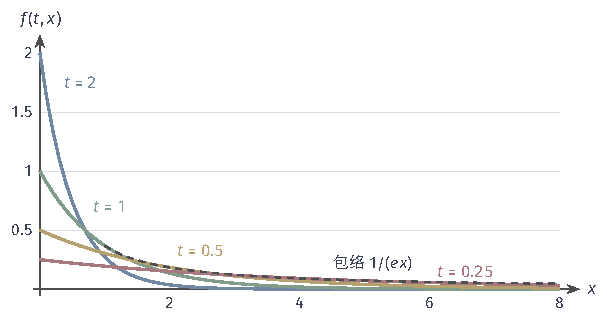
\includegraphics[width=102.807mm]{figures/02-abstract-mathematics/01-metric-and-measure/tikz/c3-parameter-continuity/figure.pdf}
\caption{含参积分中质量的逃逸。四条实线是$f(t,x)=te^{-tx}$在$t=2,1,0.5,0.25$时的图像，每条曲线下的面积都是$1$；$t$越小，质量越向右摊开。虚线是包络$\sup_tte^{-tx}=1/(ex)$（在$t=1/x$处取到，画在$x\geq1$部分），它在无穷远处不可积，所以$t=0$附近没有可积控制。}
\label{fig:integ-parameter-continuity}
\end{figure}

\subsection{积分号下求导}
\label{sec:integ-differentiation-under-integral}

\paragraph{求导定理}
现在设参数取值于开区间$T\subseteq\mathbb R$。$F$在$t$处的差商是$\int\bigl(f(x,t+h)-f(x,t)\bigr)/h\,\mathrm d\mu$，被积函数在$h\to0$时趋于$\partial_tf(x,t)$。要把极限移进积分号，同样需要给差商一个共同的可积上界；由中值定理，差商的大小由导数在参数区间上的大小控制。

\begin{theorem}[积分号下求导]
\label{thm:integ-differentiation-under-integral}
设$T\subseteq\mathbb R$是开区间，$f:X\times T\to\mathbb R$满足：
\begin{enumerate}
 \item 存在$t_0\in T$，使$f(\cdot,t_0)$可积；
 \item 存在零测集$N$，使对每个$x\notin N$，$t\mapsto f(x,t)$在$T$上可微；
 \item 存在可积函数$g\geq0$，使对每个$x\notin N$与每个$t\in T$，$\lvert\partial_tf(x,t)\rvert\leq g(x)$。
\end{enumerate}
则对每个$t\in T$，$f(\cdot,t)$可积，$F(t)=\int_Xf(x,t)\,\mathrm d\mu(x)$在$T$上可微，并且
\[
 F'(t)=\int_X\partial_tf(x,t)\,\mathrm d\mu(x).
\]
复值函数对实部与虚部分别应用即可。
\end{theorem}

\begin{proof}
对$x\notin N$，由中值定理，$\lvert f(x,t)-f(x,s)\rvert\leq g(x)\lvert t-s\rvert$对$s,t\in T$成立。取$s=t_0$，得$\lvert f(x,t)\rvert\leq\lvert f(x,t_0)\rvert+\lvert t-t_0\rvert g(x)$，右边可积，所以每个$f(\cdot,t)$可积。

固定$t\in T$，任取$h_n\to0$且$t+h_n\in T$，$h_n\neq0$。差商$q_n(x)=\bigl(f(x,t+h_n)-f(x,t)\bigr)/h_n$是可测函数，在$N$外收敛到$\partial_tf(x,t)$，所以$\partial_tf(\cdot,t)$在$N$外是可测函数列的极限，可测。由中值定理，$\lvert q_n(x)\rvert\leq g(x)$。由支配收敛定理与线性性，
\[
 \frac{F(t+h_n)-F(t)}{h_n}=\int_Xq_n\,\mathrm d\mu\to\int_X\partial_tf(x,t)\,\mathrm d\mu .
\]
对一切$h_n\to0$都成立，所以$F$在$t$处可微且导数如定理所述。
\end{proof}

导数的控制条件只需在一个参数区间内成立。若条件只在每个$t$附近的某个子区间上成立，把定理用于这些子区间，同样得到$F$在整个$T$上可微。

\begin{example}[逐阶求导]
\label{ex:integ-gamma-derivatives}
对$t>0$，$F(t)=\int_0^\infty e^{-tx}\,\mathrm dx=1/t$。固定$t_0>0$，在$T=(t_0,\infty)$上，$\lvert\partial_te^{-tx}\rvert=xe^{-tx}\leq xe^{-t_0x}$，右边在$[0,\infty)$上可积。由定理，$-\int_0^\infty xe^{-tx}\,\mathrm dx=F'(t)=-1/t^2$。同样的控制$x^ne^{-t_0x}$允许继续求导，归纳得$\int_0^\infty x^ne^{-tx}\,\mathrm dx=n!/t^{n+1}$；取$t=1$即$\int_0^\infty x^ne^{-x}\,\mathrm dx=n!$。由于$t_0>0$任意，结论对一切$t>0$成立；而在$t=0$附近控制失效，$F$本身也在那里趋于无穷。
\end{example}

\paragraph{偏导数逐点存在不等于可以交换}
定理的第3条不能省去。在$[0,\infty)$上取$f(x,t)=t^3e^{-t^2x}$，$t\in\mathbb R$。对$t\neq0$，$F(t)=t^3\cdot t^{-2}=t$；又$F(0)=0$，所以$F(t)=t$，$F'(0)=1$。另一方面，对每个$x\geq0$，
\[
 \partial_tf(x,0)=\lim_{t\to0}\frac{t^3e^{-t^2x}}t=0,
\]
于是$\int_0^\infty\partial_tf(x,0)\,\mathrm dx=0\neq1$。偏导数在每一点都存在，交换却失败了。原因是$\partial_tf(x,t)=(3t^2-2t^4x)e^{-t^2x}$在$t^2=1/x$处等于$1/(ex)$，所以在$0$的任何参数邻域内，它的上包络不小于一个在无穷远处不可积的函数；控制条件必须覆盖参数邻域，只在$t=0$处检查导数是不够的。

\subsection{变动区域上的积分}
\label{sec:integ-moving-domain}

\paragraph{变限的一元积分}
当积分区域也随参数移动时，$F(t)$的变化来自两部分：区域内部的被积函数在变，边界又新添或移除了一部分区域。先看一元的变限积分$F(t)=\int_{a(t)}^{b(t)}f(x,t)\,\mathrm dx$。

\begin{theorem}[变限积分的求导]
\label{thm:integ-variable-limits}
设$J=[\alpha,\beta]$，$T\subseteq\mathbb R$是开区间，$a,b:T\to J$可微。设$f:J\times T\to\mathbb R$连续，$\partial_tf$在$J\times T$上处处存在，并存在可积函数$g\geq0$使$\lvert\partial_tf(x,t)\rvert\leq g(x)$对一切$x\in J$、$t\in T$成立。则$F(t)=\int_{a(t)}^{b(t)}f(x,t)\,\mathrm dx$在$T$上可微，且
\[
 F'(t)=\int_{a(t)}^{b(t)}\partial_tf(x,t)\,\mathrm dx+f\bigl(b(t),t\bigr)b'(t)-f\bigl(a(t),t\bigr)a'(t).
\]
\end{theorem}

\begin{proof}
固定$t$，取$h\neq0$且$t+h\in T$，记$a=a(t)$、$a_h=a(t+h)$，$b,b_h$同理。把增量拆成三部分：
\begin{equation*}
\begin{aligned}
 F(t+h)-F(t)={}&\int_a^b\bigl(f(x,t+h)-f(x,t)\bigr)\mathrm dx\\
 &+\int_b^{b_h}f(x,t+h)\,\mathrm dx-\int_a^{a_h}f(x,t+h)\,\mathrm dx .
\end{aligned}
\end{equation*}
第一项除以$h$后，由定理~\ref{thm:integ-differentiation-under-integral}的论证（差商由$g$控制，支配收敛）趋于$\int_a^b\partial_tf(x,t)\,\mathrm dx$。

第二项来自上端点的移动。$f$在$(b,t)$处连续，对$\varepsilon>0$，当$h$足够小时，$b_h$与$b$之间的每个$x$都满足$\lvert f(x,t+h)-f(b,t)\rvert<\varepsilon$。于是
\[
 \Bigl\lvert\frac1h\int_b^{b_h}f(x,t+h)\,\mathrm dx-\frac{b_h-b}hf(b,t)\Bigr\rvert\leq\varepsilon\Bigl\lvert\frac{b_h-b}h\Bigr\rvert,
\]
而$(b_h-b)/h\to b'(t)$，所以第二项除以$h$趋于$f(b,t)b'(t)$。第三项同理趋于$f(a,t)a'(t)$。
\end{proof}

两个边界项符号相反：上端向右移动增加积分区域，下端向右移动减少积分区域。例如$F(t)=\int_0^txt\,\mathrm dx=t^3/2$，直接求导得$3t^2/2$；按定理计算，内部变化贡献$\int_0^tx\,\mathrm dx=t^2/2$，上端移动贡献$f(t,t)\cdot1=t^2$，合计$3t^2/2$，两者一致。与卷二在连续可微条件下的同一公式相比，这里只要求被积函数连续、参数导数有可积控制，内部项的交换完全由支配收敛负责；连续性只在边界点上用于读出新添部分的高度。

\paragraph{有参数的多元区域}
在$\mathbb R^d$中，区域的移动不能只用两个端点描述，需要把区域参数化。设$\Omega_0\subseteq\mathbb R^d$是开集，对每个$t\in T$，$\Phi_t:\Omega_0\to\Omega_t$是连续可微的双射，逆映射也连续可微，记$J_t(y)=\lvert\det D\Phi_t(y)\rvert$。由卷二的积分换元公式（可参考\BookChapterRef{chap:region-integrals}{卷二第21章“区域积分”}），
\[
 F(t)=\int_{\Omega_t}f(x,t)\,\mathrm dx=\int_{\Omega_0}f\bigl(\Phi_t(y),t\bigr)J_t(y)\,\mathrm dy,
\]
右端是固定区域上的积分。

于是变动区域的问题化为固定区域上的含参积分：只要对几乎每个$y$，映射$t\mapsto f(\Phi_t(y),t)J_t(y)$可微，并且这个参数导数在$T$上有与$t$无关的可积上界，就可以用定理~\ref{thm:integ-differentiation-under-integral}在积分号下求导。这里有两类条件：边界的移动由参数化$\Phi_t$的光滑性描述，被积函数的变化由支配条件控制，二者都要在使用前核对。一元情形取$\Phi_t(y)=a(t)+y(b(t)-a(t))$，$\Omega_0=(0,1)$，得到的正是上面的公式。

在$\Phi$足够光滑时，把导数写回$\Omega_t$上，并用散度定理把与区域移动有关的部分改写成边界上的通量，可以得到边界项的多元形式：它沿整个边界累计被积函数乘以边界的法向移动速度。这一改写需要边界的光滑性与散度定理，这里不展开推导。

\section{本章小结}
\label{sec:integ-summary}

本章开头问：怎样按位置给出不同的贡献再累计，累计能否与极限、依次求积和求导交换。积分按值域分层：非负简单函数的积分是“高度乘以测度”之和，与写法无关；一般非负可测函数的积分是下方简单函数积分的上确界，允许取$+\infty$，并且任何一列递增的简单逼近都能算出它。实值函数把正部与负部分开累计，只要至少一部分有限积分就存在，两部分都有限才称可积；复值函数以模的积分有限为可积条件，按实部与虚部积分。积分看不见零测集，只依赖函数的几乎处处等价类。

基本性质各有条件。非负函数的线性组合要求系数非负，并按$0\cdot(+\infty)=0$处理无穷；可积函数允许任意实系数或复系数，但只知道积分存在不足以相加。单调性可以放宽到几乎处处，复值积分不比较大小，绝对值估计则通过旋转把复积分化为实部与模的比较，并给出$\lvert\int f-\int g\rvert\leq\int\lvert f-g\rvert$。有限个不交区域的积分可加，增删零测集不改变积分，可数个区域的情形要用单调收敛定理。

与经典积分相比，有界闭区间上的有界函数黎曼可积当且仅当不连续点集零测，此时两种积分相等；$\mathbf 1_{\mathbb Q}$只有新积分。反常积分在绝对收敛时与新积分一致，条件收敛的$\sin x/x$却不是Lebesgue可积的，因为测度积分不依赖任何次序。

积分与极限的交换由尖峰例子引出：逐点收敛不足以保证积分收敛，质量可以挤进越来越窄的区间，或者摊到无界区域上。单调收敛定理处理递增的非负函数列，并给出非负级数逐项积分；Fatou引理对非负函数列给出单向估计；支配收敛定理在存在共同可积上界时交换极限与积分，并保证$\int\lvert f_n-f\rvert\to0$。

累次积分与含参积分分别给出换序与参数运算的条件。$\sigma$有限测度的乘积测度由矩形上的乘积赋值唯一确定；Tonelli定理对非负可测函数无条件换序，Fubini定理在先核对$\int\lvert f\rvert<+\infty$后对一般函数换序，截面只需几乎处处可积，例外处的内层积分取零；完备化下截面的可测性也只对几乎每个参数成立。含参积分的连续性与积分号下求导都依赖参数邻域上与参数无关的可积控制；积分区域移动时，还要加上边界移动带来的项。

微积分基本定理在绝对连续条件下联系积分与导数。可积函数的变上限积分绝对连续，几乎处处可导，导数几乎处处等于被积函数；反过来，绝对连续函数几乎处处可导、导数可积，并能由一点的函数值和导数的积分恢复。Cantor函数连续、单调、几乎处处导数为零却从$0$增到$1$，标出了恢复公式的边界。第~\ref{chap:smoothing-weak-derivatives}章在这些基础上研究卷积光滑化与弱导数，那里要用到本章的换序、积分号下求导与一维的积分恢复；换测度与沿映射换元分别在第~\ref{chap:measure-densities}章与第~\ref{chap:pushforward-measures}章展开。


\chapter{光滑逼近与弱导数}
\label{chap:smoothing-weak-derivatives}

阶跃函数在跳点没有导数，绝对值函数在原点有一个尖角，测量得到的信号还常常只在几乎处处意义下确定。对这类函数，逐点定义的导数要么在个别点失效，要么根本无从谈起：把函数在一个零测集上改值，积分不变，任意一点的函数值却可以变成任何数。

于是有两个问题。能否用光滑函数在积分意义下逼近这些函数？能否绕开逐点差商，给它们一个可以运算的“导数”？

第一个问题的回答是局部平均。把每一点的函数值换成它附近的加权平均，权重取光滑的函数，结果就是光滑的；平均范围缩小时，结果回到原函数。第二个问题的回答是把分部积分反过来用。光滑函数的导数乘测试函数再积分，等于函数本身乘测试函数的导数再积分，后者不需要函数可导，可以拿来当定义。

本章只在欧氏开集上工作，积分换序、积分号下求导、支配收敛和绝对连续函数的微积分基本定理都取自第~\ref{chap:integration}章。以弱导数的$L^p$大小为范数的Sobolev空间、它的完备性与嵌入在第~\ref{chap:sobolev-spaces}章研究；磨光在$L^p$范数下的收敛放在第~\ref{chap:function-approximation}章，本章只建立积分误差意义下的局部逼近。

\section{卷积光滑化}
\label{sec:weakd-convolution-smoothing}

阶跃函数$\mathbf 1_{(0,\infty)}$在原点断开。若把每一点的函数值换成它在一个小邻域内的加权平均，并让权重光滑地变化，得到的函数就不再有断点；邻域越小，平均值越接近原来的值。要把这个想法写成定理，先得规定哪些函数可以做局部平均、用什么函数做权重。

本章的点$x,y,z$都在欧氏空间$\mathbb R^d$中，作为积分变量使用，不加粗；$\lvert x\rvert$表示欧氏长度，$\mathrm dx$表示$d$维Lebesgue测度。$\Omega$总表示$\mathbb R^d$中的非空开集，$\operatorname{dist}(x,\Omega^{c})$表示$x$到补集$\Omega^{c}=\mathbb R^d\setminus\Omega$的距离；$\Omega=\mathbb R^d$时约定这个距离为$+\infty$。

\subsection{局部可积函数与测试函数}
\label{sec:weakd-local-integrability}

在一点附近做平均，只需要函数在这个邻域上可积，不需要它在整个区域上可积。考虑$(0,1)$上的$1/x$：它在靠近$0$处无界，整体积分发散；但在离$0$有一段距离的地方，它是有界连续函数，完全可以平均。下面的定义只要求这种局部控制。

\begin{definition}[局部可积]
\label{def:weakd-locally-integrable}
设$f$是$\Omega$上的可测函数，取实值或复值。若对每个紧集$K\subset\Omega$都有$\int_K\lvert f\rvert\,\mathrm dx<\infty$，就称$f$在$\Omega$上\term{局部可积}（locally integrable），记作$f\in L^1_{\mathrm{loc}}(\Omega)$。几乎处处相等的两个函数视为同一元素。
\end{definition}

定义只检查紧含于$\Omega$的集合，所以函数在边界附近可以任意增大。仍以$1/x$为例。$(0,1)$的紧子集$K$都落在某个$[a,b]$中，其中$0<a<b<1$，而$1/x$在其上不超过$1/a$，于是
\[
\int_K\frac{\mathrm dx}{x}\leq\frac{b-a}{a}<\infty .
\]
所以$1/x\in L^1_{\mathrm{loc}}(0,1)$。另一方面，
\[
\int_0^1\frac{\mathrm dx}{x}=+\infty ,
\]
它在$(0,1)$上不可积。

把同一个函数放到整条实轴上，紧区间$[-1,1]$上的积分就发散了，它不再局部可积。可见局部可积依赖于区域：边界在哪里，哪里就不受控制。

\paragraph{支撑与测试函数}
平均要用权重函数。为了让权重只读取区域内部的值，并且在后面的分部积分中不留下边界项，我们要求权重在边界附近恒为零。先把“恒为零的地方”说清楚。

\begin{definition}[支撑与测试函数]
\label{def:weakd-test-function}
函数$\varphi:\Omega\to\mathbb C$的\term{支撑}（support of a function）是集合$\{x\in\Omega:\varphi(x)\neq0\}$在$\mathbb R^d$中的闭包，记作$\operatorname{supp}\varphi$。$\Omega$上无穷次可微、支撑是紧集且含于$\Omega$的函数全体记作$C_c^\infty(\Omega)$，其中的函数称为\term{测试函数}（test function）。
\end{definition}

支撑是紧集并含于$\Omega$，意味着它与补集$\Omega^{c}$有正距离，因为紧集到不相交闭集的距离为正。于是存在$\delta>0$，使离边界不到$\delta$的点上测试函数恒为零。

测试函数$\varphi$在其支撑$K$上连续，因而有界。所以对$f\in L^1_{\mathrm{loc}}(\Omega)$，有
\begin{equation}
\Bigl\lvert\int_\Omega f\varphi\,\mathrm dx\Bigr\rvert\leq\Bigl(\sup_{K}\lvert\varphi\rvert\Bigr)\int_K\lvert f\rvert\,\mathrm dx<\infty .
\label{eq:weakd-local-pairing}
\end{equation}
这说明局部可积正是让“与测试函数相乘后积分”有意义的条件。改变$f$在零测集上的值不影响左端，所以这个积分读取的是几乎处处等价类的信息。

\paragraph{光滑隆起函数}
测试函数是否存在，需要构造才能回答。多项式、指数和三角函数都做不到：它们在一点的全部导数决定了整条实轴上的值，一旦在某个区间上恒为零，就处处为零。我们要找一个在某点所有导数都为零、却不恒为零的光滑函数。

令
\[
E(s)=\exp(-1/s)\quad(s>0),\qquad E(s)=0\quad(s\leq0).
\]
先看它在$s>0$处的各阶导数。对$k$归纳可以写出
\[
E^{(k)}(s)=P_k(1/s)\,\exp(-1/s),\qquad s>0,
\]
其中$P_k$是多项式。$k=0$时$P_0=1$。由$k$到$k+1$时求一次导，得到
\[
\frac{\mathrm d}{\mathrm ds}\Bigl[P_k(1/s)\,\mathrm e^{-1/s}\Bigr]
=\frac{1}{s^2}\Bigl[P_k(1/s)-P_k'(1/s)\Bigr]\mathrm e^{-1/s},
\]
方括号外的因子$s^{-2}$与方括号内的式子合起来仍是$1/s$的多项式。

再看$s\to0^+$时的行为。令$t=1/s\to+\infty$，对每个整数$m\geq0$有
\[
s^{-m}\,\mathrm e^{-1/s}=t^m\mathrm e^{-t}\to0 ,
\]
指数压过任意多项式，所以$E^{(k)}(s)\to0$（$s\to0^+$）。

最后在$s=0$处逐阶检查导数定义。设已知$E^{(k)}(0)=0$。左侧的差商为零，右侧的差商是
\[
\frac{E^{(k)}(s)-0}{s}=\frac1s\,P_k(1/s)\,\mathrm e^{-1/s}\to0 .
\]
所以$E^{(k+1)}(0)=0$。这样$E$在实轴上无穷次可微，并且在原点的全部导数为零，它的Taylor级数在原点恒为零，却不等于$E$本身。

把$s$换成$1-\lvert x\rvert^2$，得到
\begin{equation}
\psi(x)=E\bigl(1-\lvert x\rvert^2\bigr)=
\begin{cases}
\exp\Bigl(-\dfrac{1}{1-\lvert x\rvert^2}\Bigr),&\lvert x\rvert<1,\\
0,&\lvert x\rvert\geq1 .
\end{cases}
\label{eq:weakd-bump}
\end{equation}
$\lvert x\rvert^2=x_1^2+\cdots+x_d^2$是多项式，与光滑函数$E$复合后仍光滑。$\psi$在开单位球内为正，在球外为零，支撑是闭单位球。这样的函数称为\term{隆起函数}（bump function）。

隆起函数可以放到任意内点附近。设$x_0\in\Omega$，取$0<r<\operatorname{dist}(x_0,\Omega^{c})$，令
\[
\varphi(x)=\psi\Bigl(\frac{x-x_0}{r}\Bigr).
\]
它在开球$B(x_0,r)$内为正，支撑是闭球$\overline B(x_0,r)$，紧且含于$\Omega$，所以$\varphi\in C_c^\infty(\Omega)$。因此每个内点附近都有测试函数，而且可以把支撑压缩到任意小的球内。

图~\ref{fig:weakd-bump}按这三步画出构造。左图中$E$在原点左侧为零，右侧从零开始上升，接合处没有任何折痕；中图把两个这样的接合点放在$\pm1$，得到一个鼓包；右图把鼓包平移、缩小，放进区域$\Omega$内部。

\begin{BookInlineFigure}
  \centering
  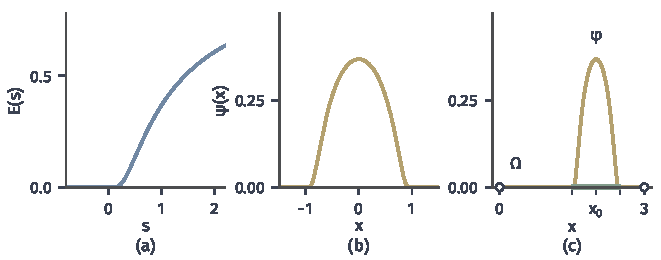
\includegraphics[width=112mm]{figures/04-spaces-measures-and-geometry/02-measure/matplotlib/weakd-bump/figure.pdf}
  \caption{隆起函数的构造，一维情形。(a)~$E(s)$在$s\leq0$处为零，在$s>0$处为$\exp(-1/s)$。(b)~隆起函数$\psi$的支撑是$[-1,1]$，峰值$\mathrm e^{-1}\approx0.368$。(c)~区域$\Omega=(0,3)$内的测试函数$\varphi(x)=\psi((x-x_0)/r)$，这里$x_0=2$，$r=0.5$；横轴上的绿色线段是支撑$[1.5,2.5]$，两个空心圆表示$\Omega$的端点不属于$\Omega$。}
  \label{fig:weakd-bump}
\end{BookInlineFigure}

\subsection{卷积}
\label{sec:weakd-convolution}

局部平均要把$f$在$x$附近的值按某个权重加起来，权重只依赖于被读取的点相对$x$的位置。这件事在数列上是熟悉的滑动平均，我们先从数列看起。

把一个双向无穷的数列看成向量$a=[\ldots,a_{-1},a_0,a_1,a_2,\ldots]$，再取一组权重$w_{-1}=w_1=\tfrac14$，$w_0=\tfrac12$，其余$w_j=0$。滑动平均把第$k$个分量换成它和两个邻居的加权平均：
\begin{equation}
b_k=\sum_{j}w_j\,a_{k-j}=\tfrac14a_{k+1}+\tfrac12a_k+\tfrac14a_{k-1}.
\label{eq:weakd-moving-average}
\end{equation}
下面用一个台阶状的向量手算一遍，它在$k\leq0$处为$0$，在$k\geq1$处为$1$。把四个相邻的下标代入式~\eqref{eq:weakd-moving-average}，得到
\[
b_{-1}=0,\quad b_0=\tfrac14,\quad b_1=\tfrac34,\quad b_2=1.
\]

台阶从一步跳变摊成了两级小台阶，如图~\ref{fig:weakd-moving-average}。权重的总和是$1$，所以常数向量经过平均不变；这里在$k\leq-1$处$b_k=0$，在$k\geq2$处$b_k=1$，正是因为这些位置的三个邻居都相同。

\begin{BookInlineFigure}
  \centering
  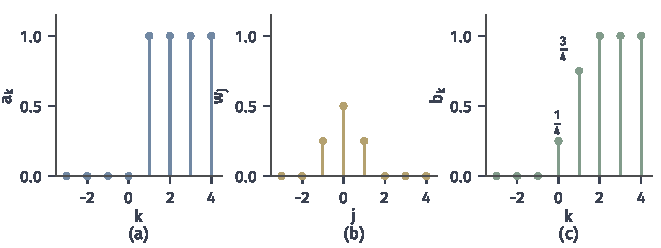
\includegraphics[width=112mm]{figures/04-spaces-measures-and-geometry/02-measure/matplotlib/weakd-moving-average/figure.pdf}
  \caption{数列上的滑动平均。(a)~台阶状的向量$a$。(b)~权重$w_{-1}=w_1=\frac14$，$w_0=\frac12$，总和为$1$。(c)~平均后的向量$b$：跳变被摊开到两个位置，离跳变较远的分量不变。}
  \label{fig:weakd-moving-average}
\end{BookInlineFigure}

现在让下标连续变化，把函数看成“每个点占一个分量”的向量。分量$a_k$变成函数值$f(x)$，权重$w_j$变成权重函数$g(z)$，求和变成积分。表~\ref{tab:weakd-dictionary}列出对应关系，其中式~\eqref{eq:weakd-moving-average}对应的连续形式就是卷积。

\begin{BookInlineTable}
  \centering
  \begin{tabular}{@{}ll@{}}
    \toprule
    数列 & 函数\\
    \midrule
    下标$k\in\mathbb Z$ & 点$x\in\mathbb R^d$\\
    分量$a_k$ & 函数值$f(x)$\\
    权重$w_j$，$\sum_jw_j=1$ & 权重函数$g(z)$，$\int g\,\mathrm dz=1$\\
    平移$k\mapsto k-j$ & 平移$x\mapsto x-z$\\
    $b_k=\sum_jw_j\,a_{k-j}$ & $(f*g)(x)=\int g(z)\,f(x-z)\,\mathrm dz$\\
    \bottomrule
  \end{tabular}
  \caption{滑动平均与卷积的对应。}
  \label{tab:weakd-dictionary}
\end{BookInlineTable}

类比有一处要改。数列的每个分量都有自己的权重，改动一个分量，平均值就可能变；函数的单个点在积分中没有权重，改动一个点不影响平均。所以卷积只读取函数的几乎处处等价类，这正是我们想要的。

\paragraph{平移与缩放的积分规则}
卷积的计算反复用到变量替换，先核对Lebesgue积分在平移、反射和缩放下怎样变化。设$h\in\mathbb R^d$，$a\neq0$，记$\lambda_d$为$d$维Lebesgue测度。

第~\ref{chap:measure}章的Lebesgue外测度是用可数个矩形覆盖的总体积取下确界得到的。矩形$R=\prod_{i}[\alpha_i,\beta_i]$平移$h$后仍是矩形，体积不变；关于原点反射后也是矩形，体积不变；乘以$a$后各边长乘$\lvert a\rvert$，体积乘$\lvert a\rvert^d$。集合$A$的覆盖与$A+h$、$-A$、$aA$的覆盖一一对应，总体积按同样的比例变化。

可测性判据中的检验集合也随之一一对应，因此可测集映成可测集，并且
\[
\lambda_d(A+h)=\lambda_d(A),\quad\lambda_d(-A)=\lambda_d(A),\quad\lambda_d(aA)=\lvert a\rvert^d\lambda_d(A).
\]

把集合的规则推广到函数。对指示函数$f=\mathbf 1_A$，有
\[
f(x-h)=\mathbf 1_{A+h}(x),\quad f(-x)=\mathbf 1_{-A}(x),\quad f(x/a)=\mathbf 1_{aA}(x),
\]
于是集合的规则就是函数的等式。由线性性推广到非负简单函数，再取递增的简单函数逼近并用单调收敛定理，得到对非负可测$f$成立的
\begin{equation}
\begin{gathered}
\int f(x-h)\,\mathrm dx=\int f(x)\,\mathrm dx,\qquad
\int f(-x)\,\mathrm dx=\int f(x)\,\mathrm dx,\\
\int f\Bigl(\frac xa\Bigr)\mathrm dx=\lvert a\rvert^d\int f(x)\,\mathrm dx .
\end{gathered}
\label{eq:weakd-translation-scaling}
\end{equation}
可积函数分正负部、实部与虚部处理，等式仍成立。缩放规则中的因子$\lvert a\rvert^d$将用来保持磨光核的总积分为$1$。

\paragraph{卷积的定义}
在$\mathbb R^d$上取两个可积函数$f,g$。我们希望对每个$x$计算
\begin{equation}
(f*g)(x)=\int_{\mathbb R^d}f(x-y)\,g(y)\,\mathrm dy .
\label{eq:weakd-convolution}
\end{equation}
右端有定义时，称$f*g$为$f$与$g$的\term{卷积}（convolution）。它把$g$当作权重，对$f$在$x-y$处的值累计。被积函数是两个可积函数之积，不一定可积，所以先要说明对哪些$x$右端有意义。

可测性要先处理。可测函数在一个Borel零测集外与某个Borel函数相等（第~\ref{chap:measure}章的完备化），先设$f,g$是Borel函数，则$(x,y)\mapsto f(x-y)g(y)$是$\mathbb R^{2d}$上的Borel函数，因为映射$(x,y)\mapsto x-y$连续。

若$f$在Borel零测集$N$之外被改值，被改动的点落在$\{(x,y):x-y\in N\}$中。这个集合对每个固定的$y$的截面是$N+y$，测度为零，由Tonelli定理它是$\mathbb R^{2d}$中的零测集。$g$的改值同样只涉及零测集$\mathbb R^d\times N'$，所以都不影响下面的积分。

\begin{theorem}[可积函数的卷积]
\label{thm:weakd-convolution-l1}
设$f,g$在$\mathbb R^d$上可积。则对几乎每个$x\in\mathbb R^d$，函数$y\mapsto f(x-y)g(y)$可积，由式~\eqref{eq:weakd-convolution}定义的$f*g$几乎处处有定义、可积，并且
\begin{equation}
\int_{\mathbb R^d}\lvert(f*g)(x)\rvert\,\mathrm dx\leq\Bigl(\int_{\mathbb R^d}\lvert f\rvert\,\mathrm dx\Bigr)\Bigl(\int_{\mathbb R^d}\lvert g\rvert\,\mathrm dx\Bigr).
\label{eq:weakd-young-l1}
\end{equation}
此外$f*g=g*f$几乎处处成立。
\end{theorem}

\begin{proof}
对非负函数$(x,y)\mapsto\lvert f(x-y)\rvert\lvert g(y)\rvert$用Tonelli定理，先对$x$积分。由式~\eqref{eq:weakd-translation-scaling}的平移规则，内层对$x$的积分等于$\int\lvert f\rvert$，与$y$无关，所以
\[
\begin{aligned}
\int\!\!\int\lvert f(x-y)\rvert\,\lvert g(y)\rvert\,\mathrm dy\,\mathrm dx
&=\int\lvert g(y)\rvert\Bigl(\int\lvert f(x-y)\rvert\,\mathrm dx\Bigr)\mathrm dy\\
&=\int\lvert f\rvert\,\mathrm dx\cdot\int\lvert g\rvert\,\mathrm dy<\infty .
\end{aligned}
\]

左端按另一种次序是$\int G(x)\,\mathrm dx$，其中
\[
G(x)=\int\lvert f(x-y)\,g(y)\rvert\,\mathrm dy .
\]
非负函数积分有限，所以$G(x)<\infty$对几乎每个$x$成立，这些$x$处$y\mapsto f(x-y)g(y)$可积。

被积函数在$\mathbb R^{2d}$上绝对可积，由Fubini定理，$x\mapsto(f*g)(x)$在例外零测集外有定义且可测（例外集上取零），并且$\lvert(f*g)(x)\rvert\leq G(x)$。对$x$积分即得式~\eqref{eq:weakd-young-l1}。

交换律来自对固定的$x$作替换$y\mapsto x-y$。它是反射与平移的复合，由式~\eqref{eq:weakd-translation-scaling}不改变积分，于是
\[
\int f(x-y)\,g(y)\,\mathrm dy=\int f(y)\,g(x-y)\,\mathrm dy .
\]
\end{proof}

两个可积性条件都不能少。若只假设$f,g$局部可积，卷积可以处处发散：$\mathbb R$上$f=g=1$时，对每个$x$都有
\[
\int_{\mathbb R}f(x-y)\,g(y)\,\mathrm dy=\int_{\mathbb R}1\,\mathrm dy=+\infty .
\]
式~\eqref{eq:weakd-young-l1}的证明正是靠两个绝对积分的乘积有限，Tonelli定理才给出几乎处处有限的内层积分。下一小节的磨光核紧支撑且有界，那时只需要$f$局部可积，因为每个$x$处的积分只读取$f$在一个紧集上的值。

下面的例子可以逐点算出，它把权重的滑动过程完整走一遍。

\begin{example}[两个盒函数的卷积]
\label{ex:weakd-box-convolution}
取$d=1$，$f=g=\mathbf 1_{[0,1]}$。由交换律，用形式$\int f(y)g(x-y)\,\mathrm dy$来算。固定$x$，$g(x-y)=1$当且仅当$x-y\in[0,1]$，也就是$y\in[x-1,x]$。所以卷积值就是两段的重叠长度：
\[
(f*g)(x)=\lambda_1\bigl([0,1]\cap[x-1,x]\bigr).
\]
当$0\leq x\leq1$时重叠区间是$[0,x]$，当$1\leq x\leq2$时重叠区间是$[x-1,1]$，其余情形没有重叠。于是
\[
(f*g)(x)=\begin{cases}x,&0\leq x\leq1,\\2-x,&1\leq x\leq2,\\0,&\text{其余情形}.\end{cases}
\]
三角形的面积是$\frac12\cdot2\cdot1=1$，恰好等于$\int f\cdot\int g=1$，式~\eqref{eq:weakd-young-l1}在这里取等号。
\end{example}

图~\ref{fig:weakd-convolution-box}中，蓝色盒子固定，黄色盒子随$x$向右滑动，绿色部分的长度就是卷积值。两个不连续的函数卷积后成为连续函数，这是卷积光滑作用的最简单表现：滑动权重的边缘越过跳点时，重叠长度是连续变化的。

\begin{BookInlineFigure}
  \centering
  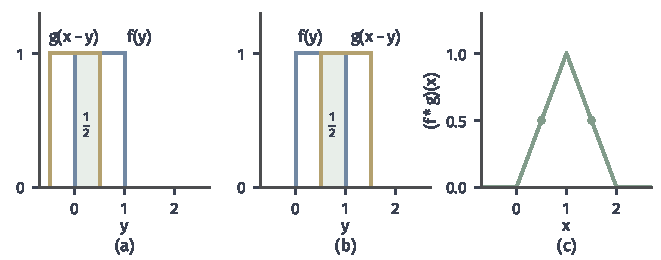
\includegraphics[width=112mm]{figures/04-spaces-measures-and-geometry/02-measure/matplotlib/weakd-convolution-box/figure.pdf}
  \caption{盒函数的卷积。(a)~$x=0.5$时固定盒子$f(y)$与滑动盒子$g(x-y)$重叠的绿色部分长$\frac12$。(b)~$x=1.5$时重叠长度同样是$\frac12$。(c)~卷积结果是$[0,2]$上的三角形，两个圆点是(a)、(b)的读数。}
  \label{fig:weakd-convolution-box}
\end{BookInlineFigure}

\subsection{局部磨光}
\label{sec:weakd-local-mollification}

现在把隆起函数归一化为权重，对局部可积函数做局部平均。由于$f$只在$\Omega$上有定义，平均的邻域必须留在$\Omega$内，这决定了磨光函数的定义域。

\paragraph{磨光核与磨光}
令$c_d=\int_{\mathbb R^d}\psi\,\mathrm dx>0$，其中$\psi$是式~\eqref{eq:weakd-bump}的隆起函数，并令
\begin{equation}
\rho(x)=c_d^{-1}\psi(x),\qquad\rho_\varepsilon(x)=\varepsilon^{-d}\rho\Bigl(\frac x\varepsilon\Bigr)\quad(\varepsilon>0).
\label{eq:weakd-mollifier}
\end{equation}
$\rho_\varepsilon$光滑、非负，支撑是闭球$\overline B(0,\varepsilon)$。由式~\eqref{eq:weakd-translation-scaling}的缩放规则，
\[
\int\rho_\varepsilon\,\mathrm dx=\varepsilon^{-d}\cdot\varepsilon^d\int\rho\,\mathrm dx=1 .
\]

$\varepsilon$减小时支撑收缩，高度按$\varepsilon^{-d}$增大，总积分保持为$1$。下面的论证只用到$\rho$光滑、非负、积分为$1$并支撑于闭单位球，任何满足这些条件的核都可以代替它；我们把这类函数称为\term{磨光核}（mollifier）。

一维时$c_1\approx0.4440$，峰值$\rho_\varepsilon(0)\approx0.829/\varepsilon$。后面的手算还要用到$\rho$的两个矩：
\[
m_1=\int_{-1}^{1}\lvert u\rvert\rho(u)\,\mathrm du\approx0.3345,\qquad
m_2=\int_{-1}^{1}u^2\rho(u)\,\mathrm du\approx0.1581 .
\]
这些数值由数值积分得到。$\rho$是偶函数，所以$\int u\rho(u)\,\mathrm du=0$。

平均的邻域要留在$\Omega$内，因此只能在离边界足够远的点上做平均。记
\[
\Omega_\varepsilon=\{x\in\Omega:\operatorname{dist}(x,\Omega^{c})>\varepsilon\},
\]
它是开集。对$f\in L^1_{\mathrm{loc}}(\Omega)$与$x\in\Omega_\varepsilon$，闭球$\overline B(x,\varepsilon)$是$\Omega$内的紧集，定义
\begin{equation}
\begin{aligned}
f_\varepsilon(x)&=\int_\Omega\rho_\varepsilon(x-y)\,f(y)\,\mathrm dy\\
&=\int_{\lvert z\rvert\leq\varepsilon}\rho_\varepsilon(z)\,f(x-z)\,\mathrm dz ,\qquad x\in\Omega_\varepsilon ,
\end{aligned}
\label{eq:weakd-mollification}
\end{equation}
称为$f$的\term{磨光}（mollification）。

被积函数在紧集$\overline B(x,\varepsilon)$外为零，由式~\eqref{eq:weakd-local-pairing}积分有限；第二个等号是替换$z=x-y$。因为$\rho_\varepsilon\geq0$且$\int\rho_\varepsilon=1$，$f_\varepsilon(x)$是$f$在球$B(x,\varepsilon)$上的加权平均，权重集中在中心附近。$\Omega=\mathbb R^d$且$f$可积时，$f_\varepsilon=f*\rho_\varepsilon$就是上一小节的卷积。

图~\ref{fig:weakd-interior}(a)说明为什么定义域要缩小：点$x$的平均球完全落在$\Omega$内，可以计算；点$x'$的平均球越过了边界，要用到$f$没有定义的地方。

\begin{BookInlineFigure}
  \centering
  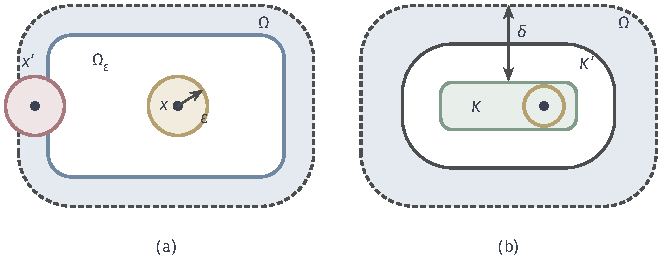
\includegraphics[width=112mm]{figures/04-spaces-measures-and-geometry/02-measure/tikz/weakd-interior/figure.pdf}
  \caption{磨光的定义域与局部逼近中的紧集。虚线是开集$\Omega$的边界。(a)~白色区域是$\Omega_\varepsilon$，灰蓝色环带上的点离边界不超过$\varepsilon$。黄色球$B(x,\varepsilon)$留在$\Omega$内，红色球越出$\Omega$，所以$x'\notin\Omega_\varepsilon$。(b)~紧集$K$（绿色）到$\Omega^{c}$的距离为$\delta$，$K'$是$K$的$\delta/2$邻域。半径小于$\delta/2$的黄色球以$K$中点为心时，都留在$K'$内。}
  \label{fig:weakd-interior}
\end{BookInlineFigure}

\paragraph{磨光函数的光滑性}
磨光把$x$只放在核里，被积的$f(y)$与$x$无关。所以对$x$求导时，可以把导数全部移到光滑的核上；需要检查的只是积分号下求导的条件。

\begin{theorem}[磨光函数光滑]
\label{thm:weakd-mollification-smooth}
设$f\in L^1_{\mathrm{loc}}(\Omega)$，$\varepsilon>0$。则$f_\varepsilon\in C^\infty(\Omega_\varepsilon)$，并且对每个多重指标$\alpha$，
\begin{equation}
\partial^\alpha f_\varepsilon(x)=\int_\Omega(\partial^\alpha\rho_\varepsilon)(x-y)\,f(y)\,\mathrm dy ,\qquad x\in\Omega_\varepsilon .
\label{eq:weakd-mollifier-derivative}
\end{equation}
这里\term{多重指标}（multi-index）$\alpha=(\alpha_1,\ldots,\alpha_d)$是非负整数组，$\lvert\alpha\rvert=\alpha_1+\cdots+\alpha_d$称为它的阶数，$\partial^\alpha$表示依次对第$j$个坐标求$\alpha_j$次偏导；$\alpha=0$时$\partial^\alpha$是恒等运算。
\end{theorem}

\begin{proof}
固定$x_0\in\Omega_\varepsilon$，取$r>0$使$\operatorname{dist}(x_0,\Omega^{c})>\varepsilon+2r$，再令$K=\overline B(x_0,\varepsilon+r)$，它是$\Omega$内的紧集。对$x\in B(x_0,r)$，若$\rho_\varepsilon(x-y)\neq0$，则$\lvert y-x\rvert<\varepsilon$，从而$y\in K$。因此在这个参数邻域内，被积函数可以写成$\rho_\varepsilon(x-y)f(y)\mathbf 1_K(y)$。

先求一个坐标方向的偏导数。对固定的$y$，$x\mapsto\rho_\varepsilon(x-y)f(y)$光滑，对$x_j$的偏导数是$(\partial_j\rho_\varepsilon)(x-y)f(y)$，其绝对值不超过
\[
M_j\,\lvert f(y)\rvert\,\mathbf 1_K(y),\qquad M_j=\sup_{\mathbb R^d}\lvert\partial_j\rho_\varepsilon\rvert<\infty .
\]
这个上界与$x\in B(x_0,r)$无关，并且由$f$局部可积而可积。沿第$j$个坐标的参数区间应用第~\ref{chap:integration}章的积分号下求导定理，得到式~\eqref{eq:weakd-mollifier-derivative}在$\lvert\alpha\rvert=1$时成立。

右端仍是同一形式的积分，只是核换成了光滑紧支撑函数$\partial_j\rho_\varepsilon$，支撑仍在$\overline B(0,\varepsilon)$内。对阶数归纳，重复上面的论证即得全部偏导数存在并满足式~\eqref{eq:weakd-mollifier-derivative}。

每个偏导数又是这种积分，被积函数关于$x$连续，并被同一个可积函数控制，由含参积分的连续性定理，它在$B(x_0,r)$上连续。$x_0$任意，所以$f_\varepsilon\in C^\infty(\Omega_\varepsilon)$。
\end{proof}

光滑性完全来自核，与$f$本身是否连续无关。下面在一维手算$f(x)=\lvert x\rvert$的磨光，$\Omega=\mathbb R$，看光滑化具体做了什么。

设$x\geq\varepsilon$。此时$\lvert z\rvert\leq\varepsilon$推出$x-z\geq0$，所以$\lvert x-z\rvert=x-z$。代入式~\eqref{eq:weakd-mollification}，并用$\int\rho_\varepsilon=1$、$\int z\rho_\varepsilon(z)\,\mathrm dz=0$，得到
\[
f_\varepsilon(x)=\int_{\lvert z\rvert\leq\varepsilon}\rho_\varepsilon(z)\,(x-z)\,\mathrm dz=x .
\]
$x\leq-\varepsilon$时同理得$f_\varepsilon(x)=-x$，所以在$\lvert x\rvert\geq\varepsilon$处磨光没有改变函数。

尖点处的值是$\rho_\varepsilon$的一阶矩。取$x=0$，再作替换$z=\varepsilon u$，得到
\[
f_\varepsilon(0)=\int_{\lvert z\rvert\leq\varepsilon}\rho_\varepsilon(z)\,\lvert z\rvert\,\mathrm dz=\varepsilon m_1 .
\]
$\varepsilon=0.5$时这个值约为$0.167$，图~\ref{fig:weakd-mollifier}(b)标出了它。同样的计算用于符号函数：在$\lvert x\rvert\geq\varepsilon$处，它的磨光等于自身；在原点，被积函数是奇函数，磨光值为$0$。

\begin{BookInlineFigure}
  \centering
  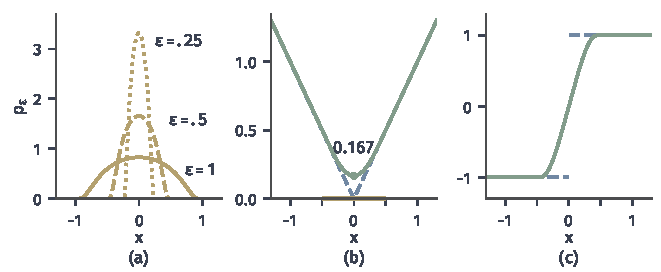
\includegraphics[width=112mm]{figures/04-spaces-measures-and-geometry/02-measure/matplotlib/weakd-mollifier/figure.pdf}
  \caption{一维磨光。(a)~磨光核$\rho_\varepsilon$，$\varepsilon=1,0.5,0.25$：支撑为$[-\varepsilon,\varepsilon]$，峰值约$0.829/\varepsilon$，面积均为$1$。(b)~$\lvert x\rvert$（蓝色虚线）与它的磨光（绿色实线），$\varepsilon=0.5$：尖点被抹平，原点值约$0.167$，横轴上黄色线段是改动发生的范围$[-\varepsilon,\varepsilon]$，其外两者重合。(c)~$\operatorname{sgn}x$与它的磨光，$\varepsilon=0.5$：后者光滑地从$-1$升到$1$，恰好是(b)中绿色曲线的导数。}
  \label{fig:weakd-mollifier}
\end{BookInlineFigure}

\subsection{平移的积分连续性}
\label{sec:weakd-translation-continuity}

磨光值$f_\varepsilon(x)$是$f(x-z)$在$\lvert z\rvert\leq\varepsilon$上的平均，所以$f_\varepsilon-f$由“把$f$平移一小段后与原来差多少”控制。逐点看，平移误差可以很大：阶跃函数平移后，跳点附近的值从$0$变成$1$。但改变的只是一段长度为$\lvert h\rvert$的区间，积分误差仍然小。

图~\ref{fig:weakd-translation}(a)画的是$\mathbf 1_{[0,1]}$平移$h=0.2$的情形。在两侧的红色条带上，逐点误差都等于$1$，一点也不小；但条带总宽只有$2h=0.4$，积分误差就是$0.4$，随$h$趋于零。下面要证明，对每个可积函数，平移引起的积分误差都随平移量趋于零。

\paragraph{集合的开集外逼近与紧集内逼近}
可积函数可以由简单函数逼近，简单函数由有限测度集合的指示函数组成。所以问题先归结为集合：一个有限测度可测集能否用一些矩形的有限并很好地近似。下面先从外测度的定义出发，用开集从外面、用紧集从里面夹住这个集合。

\begin{lemma}[Lebesgue测度的外逼近与内逼近]
\label{lem:weakd-regularity}
设$A\subset\mathbb R^d$可测且$\lambda_d(A)<\infty$，$\eta>0$。则存在开集$U\supset A$与紧集$K\subset A$，使$\lambda_d(U\setminus A)<\eta$且$\lambda_d(A\setminus K)<\eta$。
\end{lemma}

\begin{proof}
先做外逼近。按外测度的定义，存在可数个矩形$R_k$覆盖$A$且$\sum_k\lambda_d(R_k)<\lambda_d(A)+\eta/2$。把每个$R_k$的各边略微向外延伸，得到包含它的开矩形$R_k'$，并使
\[
\lambda_d(R_k')<\lambda_d(R_k)+\eta\,2^{-k-1}.
\]
令$U=\bigcup_kR_k'$，它是开集且包含$A$，并且$\lambda_d(U)<\lambda_d(A)+\eta$。由于$\lambda_d(A)$有限，得
\[
\lambda_d(U\setminus A)=\lambda_d(U)-\lambda_d(A)<\eta .
\]

再做内逼近。令$A_m=A\cap[-m,m]^d$，它们递增到$A$，由测度的从下连续性与$\lambda_d(A)<\infty$，可取$m$使$\lambda_d(A\setminus A_m)<\eta/2$。记$Q=[-m,m]^d$，对有界可测集$Q\setminus A_m$用外逼近，得到开集$V\supset Q\setminus A_m$，使
\[
\lambda_d\bigl(V\setminus(Q\setminus A_m)\bigr)<\eta/2 .
\]

令$K=Q\setminus V$，它是有界闭集，因而紧。由$V\supset Q\setminus A_m$可知$K\subset A_m\subset A$。又
\[
A_m\setminus K=A_m\cap V\subset V\setminus(Q\setminus A_m),
\]
所以
\[
\lambda_d(A\setminus K)\leq\lambda_d(A\setminus A_m)+\lambda_d(A_m\setminus K)<\eta .
\]
\end{proof}

两种逼近配合起来，就能用矩形的有限并逼近$A$。$\mathbb R^d$中的开集$U$是可数个开矩形之并：$U$中每点都落在某个端点为有理数、整个含于$U$的开矩形里，而这样的矩形只有可数个。紧集$K\subset U$被这些开矩形覆盖，由紧性可取出有限个$R_1,\ldots,R_N$覆盖$K$。

令$E=R_1\cup\cdots\cup R_N$，则$K\subset E\subset U$。于是$A$与$E$的对称差$A\triangle E=(A\setminus E)\cup(E\setminus A)$满足
\begin{equation}
\lambda_d(A\triangle E)\leq\lambda_d(A\setminus K)+\lambda_d(U\setminus A)<2\eta .
\label{eq:weakd-box-approx}
\end{equation}
外逼近负责让近似集合不多出太多测度，紧集内逼近则保证只需有限个矩形；有限性在下面估计平移误差时是必需的。

\paragraph{平移误差趋零}
单个矩形的平移误差可以直接计算。设$R=\prod_{i=1}^d[\alpha_i,\beta_i]$，边长$\ell_i=\beta_i-\alpha_i$，平移量$h=(h_1,\ldots,h_d)$。我们要估计$R$与$R+h$的对称差。

先看$(R+h)\setminus R$中的点$x$。这时$x-h\in R$而$x\notin R$，所以存在某个坐标$i$使$x_i\notin[\alpha_i,\beta_i]$。又$x_i-h_i\in[\alpha_i,\beta_i]$，所以$x_i$落在$[\alpha_i,\beta_i]$外侧紧邻的一段宽度不超过$\lvert h_i\rvert$的区间内，其余坐标$x_j$落在长度为$\ell_j$的区间$[\alpha_j+h_j,\beta_j+h_j]$内。于是$(R+h)\setminus R$被$d$块矩形盖住，第$i$块的体积不超过$\lvert h_i\rvert\prod_{j\neq i}\ell_j$。

对$R\setminus(R+h)$把$R$与$R+h$的角色互换，得到同样的估计。两部分相加，得到
\begin{equation}
\begin{aligned}
\int\lvert\mathbf 1_R(x-h)-\mathbf 1_R(x)\rvert\,\mathrm dx&=\lambda_d\bigl((R+h)\triangle R\bigr)\\
&\leq2\sum_{i=1}^d\lvert h_i\rvert\prod_{j\neq i}\ell_j ,
\end{aligned}
\label{eq:weakd-box-translation}
\end{equation}
右端随$h\to0$趋于零。一维时空积等于$1$，右端是$2\lvert h\rvert$，就是图~\ref{fig:weakd-translation}(a)的两个条带。

用二维的数验证一下。下面取矩形的边长和平移量为
\[
\ell_1=2,\quad\ell_2=1,\quad h=(0.2,\,0.1).
\]
重叠部分$R\cap(R+h)$是$1.8\times0.9$的矩形，面积$1.62$。于是实际的对称差是
\[
\lambda_2\bigl(R\triangle(R+h)\bigr)=2(2-1.62)=0.76 .
\]
式~\eqref{eq:weakd-box-translation}的右端是$2(0.2\cdot1+0.1\cdot2)=0.8$，确实不小于$0.76$，多出的部分来自四块条带在角上的重复计算，见图~\ref{fig:weakd-translation}(b)。

\begin{BookInlineFigure}
  \centering
  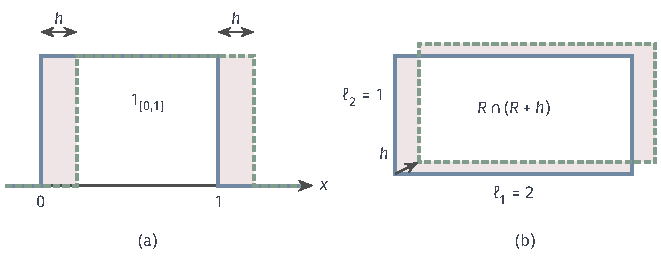
\includegraphics[width=112mm]{figures/04-spaces-measures-and-geometry/02-measure/tikz/weakd-translation/figure.pdf}
  \caption{平移引起的积分误差。蓝色实线为原函数或原矩形，绿色虚线为平移后的结果，红色区域是两者不相同的部分。(a)~$\mathbf 1_{[0,1]}$平移$h=0.2$，两侧条带上逐点误差都是$1$，积分误差为$2h=0.4$。(b)~二维矩形$R$平移$h=(0.2,0.1)$，红色部分是对称差，面积$0.76$。}
  \label{fig:weakd-translation}
\end{BookInlineFigure}

有了矩形的情形，就可以处理一般的可积函数：用矩形的有限并逼近，逼近误差和平移误差分开估计。

\begin{theorem}[平移的积分连续性]
\label{thm:weakd-translation-continuity}
设$F$在$\mathbb R^d$上可积。则
\begin{equation}
\omega_F(h):=\int_{\mathbb R^d}\lvert F(x-h)-F(x)\rvert\,\mathrm dx\to0\qquad(h\to0).
\label{eq:weakd-translation-modulus}
\end{equation}
\end{theorem}

\begin{proof}
任给$\eta>0$。第一步，用阶梯函数逼近$F$。对$F$的实部、虚部的正部与负部分别取递增的非负简单函数逼近，由单调收敛定理，可以得到简单函数$s$，满足$\int\lvert F-s\rvert<\eta$。把$s$写成不同非零值的标准形式
\[
s=\sum_{i=1}^mc_i\mathbf 1_{A_i},
\]
其中$A_i$互不相交。$s$可积，所以每个$\lambda_d(A_i)<\infty$。

由式~\eqref{eq:weakd-box-approx}，对每个$i$取矩形的有限并$E_i$，使$\lambda_d(A_i\triangle E_i)<\eta/(m\lvert c_i\rvert)$，并令$u=\sum_ic_i\mathbf 1_{E_i}$。两个指示函数之差的绝对值正是对称差的指示函数，所以$\int\lvert s-u\rvert<\eta$，从而
\[
\int\lvert F-u\rvert\,\mathrm dx<2\eta .
\]

第二步，比较三项。由三角不等式，
\[
\begin{aligned}
\lvert F(x-h)-F(x)\rvert\leq{}&\lvert F(x-h)-u(x-h)\rvert+\lvert u(x-h)-u(x)\rvert\\
&+\lvert u(x)-F(x)\rvert .
\end{aligned}
\]
对$x$积分。第一项由平移规则~\eqref{eq:weakd-translation-scaling}等于$\int\lvert F-u\rvert$，于是
\[
\omega_F(h)<4\eta+\omega_u(h).
\]

第三步，估计$\omega_u(h)$。设$E_i=R_{i,1}\cup\cdots\cup R_{i,N_i}$。若$\mathbf 1_{E_i}(x-h)\neq\mathbf 1_{E_i}(x)$，则$x-h$与$x$中恰有一个属于$E_i$，属于的那个落在某个$R_{i,k}$中而另一个不在其中，所以
\[
\lvert\mathbf 1_{E_i}(x-h)-\mathbf 1_{E_i}(x)\rvert\leq\sum_{k=1}^{N_i}\lvert\mathbf 1_{R_{i,k}}(x-h)-\mathbf 1_{R_{i,k}}(x)\rvert .
\]

积分并乘以$\lvert c_i\rvert$求和，得到
\[
\omega_u(h)\leq\sum_i\lvert c_i\rvert\sum_k\omega_{\mathbf 1_{R_{i,k}}}(h).
\]
这是有限和，由式~\eqref{eq:weakd-box-translation}，右端随$h\to0$趋于零。因此$h$足够小时$\omega_F(h)<5\eta$，而$\eta$任意。
\end{proof}

定理只控制积分误差，不控制逐点误差。图~\ref{fig:weakd-translation}(a)中对每个$h\neq0$都有点使误差等于$1$，而积分误差是$2\lvert h\rvert$，这种差别在阶跃函数上不会消失。下一小节需要的恰好只是积分误差。

\subsection{磨光的局部逼近}
\label{sec:weakd-local-approximation}

现在回到磨光函数。我们只在离边界有正距离的紧集上比较$f_\varepsilon$与$f$，因为靠近边界时磨光半径必须随之缩小。思路是把$f$截成一个可积函数，使磨光在紧集上只读取这个截断函数，然后把误差写成平移误差的平均。

\begin{theorem}[磨光的局部积分逼近]
\label{thm:weakd-local-approximation}
设$f\in L^1_{\mathrm{loc}}(\Omega)$，$K\subset\Omega$是非空紧集，$\delta=\operatorname{dist}(K,\Omega^{c})>0$。则当$0<\varepsilon<\delta$时$K\subset\Omega_\varepsilon$，并且
\begin{equation}
\int_K\lvert f_\varepsilon(x)-f(x)\rvert\,\mathrm dx\to0\qquad(\varepsilon\to0).
\label{eq:weakd-local-approximation}
\end{equation}
\end{theorem}

\begin{proof}
令$\delta_0=\min\{\delta,1\}$，这样$\Omega=\mathbb R^d$时$\delta=+\infty$的情形也包括在内。再令
\[
K'=\{x:\operatorname{dist}(x,K)\leq\delta_0/2\}.
\]
$K'$是有界闭集，并且离$\Omega^{c}$至少$\delta_0/2$，所以是$\Omega$内的紧集。令$F=f\mathbf 1_{K'}$，并在$\Omega$外取零，则$F$在$\mathbb R^d$上可积。这正是图~\ref{fig:weakd-interior}(b)的设置。

当$x\in K$、$\varepsilon<\delta_0/2$、$\lvert z\rvert\leq\varepsilon$时，$x-z\in K'$，所以$f(x-z)=F(x-z)$，并且$f(x)=F(x)$。利用$\int\rho_\varepsilon=1$把$f(x)$也写成平均，得到
\[
f_\varepsilon(x)-f(x)=\int_{\lvert z\rvert\leq\varepsilon}\rho_\varepsilon(z)\bigl(F(x-z)-F(x)\bigr)\,\mathrm dz ,\qquad x\in K .
\]

取绝对值、对$x\in K$积分，再对非负被积函数用Tonelli定理交换次序，得
\[
\begin{aligned}
\int_K\lvert f_\varepsilon-f\rvert\,\mathrm dx
&\leq\int_{\lvert z\rvert\leq\varepsilon}\rho_\varepsilon(z)\Bigl(\int_{\mathbb R^d}\lvert F(x-z)-F(x)\rvert\,\mathrm dx\Bigr)\mathrm dz\\
&\leq\sup_{\lvert z\rvert\leq\varepsilon}\omega_F(z).
\end{aligned}
\]
最后一步用了$\rho_\varepsilon\geq0$与$\int\rho_\varepsilon=1$：非负权重的平均不超过被平均量的上确界。由定理~\ref{thm:weakd-translation-continuity}，右端随$\varepsilon\to0$趋于零。
\end{proof}

证明的关键是核非负且积分为$1$：误差$f_\varepsilon-f$本身就是平移误差的加权平均，权重的总量为$1$，所以平均误差被最坏的小平移误差控制。若核取负值，权重绝对值的总积分可能大于$1$，同样的估计要多出一个因子；若核的积分不为$1$，常数函数的磨光就不再等于自身。

\begin{example}[阶跃函数的磨光误差]
\label{ex:weakd-step-mollification}
在$\Omega=(-1,1)$上取$H=\mathbf 1_{(0,1)}$，$K=[-1/2,1/2]$，并设$\varepsilon<1/2$。由式~\eqref{eq:weakd-mollification}，对$x\in K$有
\[
H_\varepsilon(x)=\int_{z<x}\rho_\varepsilon(z)\,\mathrm dz .
\]
所以在$x\leq-\varepsilon$处$H_\varepsilon=0$，在$x\geq\varepsilon$处$H_\varepsilon=1$，只在$(-\varepsilon,\varepsilon)$内取中间值。积分误差只来自这一段：
\[
\int_K\lvert H_\varepsilon-H\rvert\,\mathrm dx=\int_{-\varepsilon}^0H_\varepsilon\,\mathrm dx+\int_0^\varepsilon(1-H_\varepsilon)\,\mathrm dx .
\]

核是偶函数，所以$H_\varepsilon(-x)=1-H_\varepsilon(x)$，上式两项相等。又$x>0$时，$1-H_\varepsilon(x)$就是$\rho_\varepsilon$在$[x,\varepsilon]$上的积分，用Tonelli定理交换次序，得到
\[
\int_0^\varepsilon\!\!\int_x^\varepsilon\rho_\varepsilon(z)\,\mathrm dz\,\mathrm dx
=\int_0^\varepsilon z\,\rho_\varepsilon(z)\,\mathrm dz
=\frac{\varepsilon m_1}{2}.
\]
两项相加，积分误差恰好是
\[
\int_K\lvert H_\varepsilon-H\rvert\,\mathrm dx=\varepsilon m_1 .
\]
$\varepsilon=0.5,0.25,0.1$时分别约为$0.167,0.084,0.033$。

另一方面，核的对称性给出$H_\varepsilon(0)=\tfrac12$。当$x\to0^+$时$H_\varepsilon(x)\to\tfrac12$而$H(x)=1$，所以误差的上确界不小于$\tfrac12$；又在$K$上处处有$\lvert H_\varepsilon-H\rvert\leq\tfrac12$，因此上确界恰为$\tfrac12$，与$\varepsilon$无关。
\end{example}

图~\ref{fig:weakd-step-error}对比了这两种误差。曲线越来越陡，积分误差线性地趋于零；但最大误差始终停在$\tfrac12$，因为光滑函数要连续地穿过跳跃。

\begin{BookInlineFigure}
  \centering
  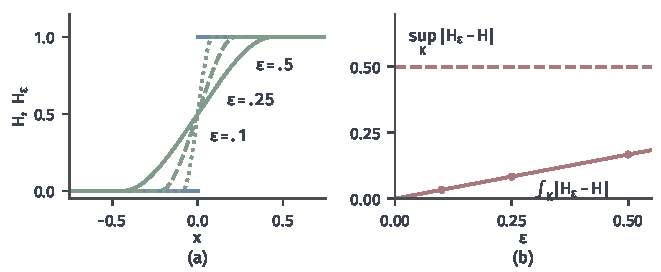
\includegraphics[width=112mm]{figures/04-spaces-measures-and-geometry/02-measure/matplotlib/weakd-step-error/figure.pdf}
  \caption{阶跃函数的磨光误差。(a)~蓝色为阶跃函数$H$，绿色为$H_\varepsilon$，$\varepsilon=0.5,0.25,0.1$依次由实线、虚线、点线表示，三条曲线都通过$(0,\tfrac12)$。(b)~$K=[-\tfrac12,\tfrac12]$上的两种误差：积分误差$\varepsilon m_1$（实线，圆点对应三个$\varepsilon$）随$\varepsilon$线性趋零，最大误差（虚线）保持为$\tfrac12$。}
  \label{fig:weakd-step-error}
\end{BookInlineFigure}

\subsection{测试函数判别}
\label{sec:weakd-test-criterion}

有限维空间里，判断一个向量是否为零，可以逐个看它在基向量上的分量：若$\langle v,e_k\rangle=0$对每个$k$成立，则$v=0$。函数的情形有类似的问题：若$h$与每个测试函数相乘后的积分都为零，$h$是否为零？

类比要作一处调整。函数“在一点的分量”$h(x)$无法用积分读出，因为单点没有测度；测试函数是一支有宽度的探针，读到的是$h$在一小块区域上的加权平均。图~\ref{fig:weakd-test-probe}说明单支探针可能什么都读不到：宽探针同时盖住正负两部分，读数为零；把探针收窄到正的部分，读数就变成正数。

\begin{BookInlineFigure}
  \centering
  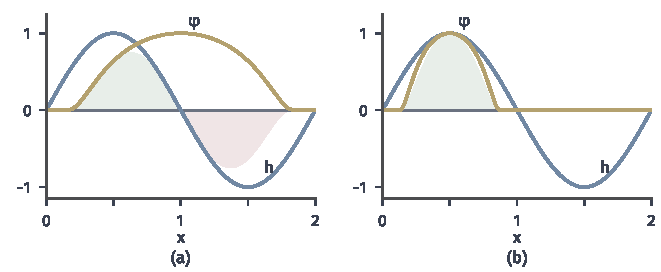
\includegraphics[width=112mm]{figures/04-spaces-measures-and-geometry/02-measure/matplotlib/weakd-test-probe/figure.pdf}
  \caption{测试函数作为探针。蓝色为$h(x)=\sin\pi x$，黄色为测试函数$\varphi$，填充部分是乘积$h\varphi$，绿色为正、红色为负。(a)~$\varphi$以$x=1$为中心、半径$0.9$，正负部分相消，$\int h\varphi=0$。(b)~$\varphi$以$x=0.5$为中心、半径$0.4$，$\int h\varphi\approx0.425$。}
  \label{fig:weakd-test-probe}
\end{BookInlineFigure}

积分看不见零测集上的差别，所以至多能期望几乎处处为零。磨光给出了肯定的回答，因为磨光值本身就是一个测试积分。

\begin{theorem}[测试函数判别]
\label{thm:weakd-test-criterion}
设$h\in L^1_{\mathrm{loc}}(\Omega)$，且对所有$\varphi\in C_c^\infty(\Omega)$都有$\int_\Omega h\varphi\,\mathrm dx=0$。则$h=0$在$\Omega$上几乎处处成立。
\end{theorem}

\begin{proof}
固定$\varepsilon>0$与$x\in\Omega_\varepsilon$。函数$\varphi_x(y)=\rho_\varepsilon(x-y)$光滑，支撑是闭球$\overline B(x,\varepsilon)$，它紧且含于$\Omega$，所以$\varphi_x\in C_c^\infty(\Omega)$。由假设，
\[
h_\varepsilon(x)=\int_\Omega h\,\varphi_x\,\mathrm dy=0 .
\]
也就是说，$h_\varepsilon$在$\Omega_\varepsilon$上恒为零。

取紧集$K\subset\Omega$。当$\varepsilon<\operatorname{dist}(K,\Omega^{c})$时，由定理~\ref{thm:weakd-local-approximation}，
\[
\int_K\lvert h\rvert\,\mathrm dx=\int_K\lvert h-h_\varepsilon\rvert\,\mathrm dx\to0 .
\]
左端与$\varepsilon$无关，所以$\int_K\lvert h\rvert=0$，即$h=0$在$K$上几乎处处成立。

最后用可数个紧集填满$\Omega$。令
\[
K_m=\{x\in\Omega:\lvert x\rvert\leq m,\ \operatorname{dist}(x,\Omega^{c})\geq1/m\},\qquad m=1,2,\ldots .
\]
它们是$\Omega$内的紧集，并且并集为$\Omega$：每个$x\in\Omega$到补集的距离为正，$m$足够大时$x\in K_m$。可数个零测集之并仍是零测集，所以$h=0$在$\Omega$上几乎处处成立。
\end{proof}

最后一步不能省。每个紧集上的结论只排除该紧集上的非零部分；开集一般不是紧集，需要用可数个内部紧集把它填满，并依靠可数可加性把各处的零测例外合在一起。复值的$h$不需要分开实部与虚部，因为定理~\ref{thm:weakd-local-approximation}对复值函数同样成立。

把判别法用于两个函数之差，就得到识别结论：若$f,g\in L^1_{\mathrm{loc}}(\Omega)$对所有测试函数满足$\int f\varphi=\int g\varphi$，则$f=g$几乎处处。因此，一个局部可积函数的几乎处处等价类，完全由它与全部测试函数的积分值决定，正如有限维向量由它在基上的分量决定。这一结论将保证下一节的弱导数不会有两个本质不同的候选。

\section{弱导数}
\label{sec:weakd-weak-derivatives}

绝对值函数$\lvert x\rvert$在原点没有导数，但除了这一点以外，它的导数$\operatorname{sgn}x$处处存在，而且一个点并不承载长度。阶跃函数$\mathbf 1_{(0,\infty)}$也只在原点没有导数，其余各点导数都是零，可它在原点确实有一次变化。逐点导数分不清这两种情形，我们改用积分来描述变化。

\subsection{经典导数的测试恒等式}
\label{sec:weakd-test-identity}

先在有限维看导数怎样“转移”。对数列定义前向差分$(Da)_k=a_{k+1}-a_k$，并取只有有限个非零分量的权重$w$。把求和重新分组，可得
\[
\sum_k(a_{k+1}-a_k)\,w_k=-\sum_ka_k\,(w_k-w_{k-1}).
\]
这是矩阵转置的关系：差分算子$D$从$a$转到$w$时变成它的转置，转置是负的后向差分，负号由此而来。

下面用一组数据核对一下，取
\[
a_k=k^2,\qquad w_2=1,\quad w_3=2,\quad\text{其余}\ w_k=0 .
\]
左端是$(9-4)\cdot1+(16-9)\cdot2=19$。右端只有$k=2,3,4$三项非零，等于$-[4\cdot1+9\cdot1+16\cdot(-2)]=19$。

$w$只有有限个非零分量，所以重新分组时没有边界项。函数的情形也一样：设$f\in C^1(\Omega)$，$\varphi\in C_c^\infty(\Omega)$，我们把$\int_\Omega(\partial_jf)\varphi$中的导数从$f$转到$\varphi$上。一元分部积分会留下端点项，而测试函数在边界附近恒为零，可以期望这些端点项全部消失。

\begin{lemma}[测试恒等式]
\label{lem:weakd-integration-by-parts}
设$f\in C^1(\Omega)$，$\varphi\in C_c^\infty(\Omega)$，$1\leq j\leq d$。则
\begin{equation}
\int_\Omega(\partial_jf)\,\varphi\,\mathrm dx=-\int_\Omega f\,\partial_j\varphi\,\mathrm dx .
\label{eq:weakd-integration-by-parts}
\end{equation}
更一般地，若$f\in C^k(\Omega)$，则对每个阶数$\lvert\alpha\rvert\leq k$的多重指标$\alpha$，
\begin{equation}
\int_\Omega(\partial^\alpha f)\,\varphi\,\mathrm dx=(-1)^{\lvert\alpha\rvert}\int_\Omega f\,\partial^\alpha\varphi\,\mathrm dx .
\label{eq:weakd-repeated-parts}
\end{equation}
\end{lemma}

\begin{proof}
令$u=f\varphi$，在$\Omega$外补成零。$u$在$\Omega$内是$C^1$的；$\operatorname{supp}\varphi$是$\Omega$内的紧集，它的某个邻域之外$u$恒为零，所以补零后$u$是$\mathbb R^d$上紧支撑的$C^1$函数。取一个包含$\operatorname{supp}\varphi$的大矩形$Q=\prod_i[a_i,b_i]$，使$\operatorname{supp}\varphi$在$Q$的内部。

固定除第$j$个以外的坐标，沿第$j$个方向用一元微积分基本定理，得到
\[
\int_{a_j}^{b_j}\partial_ju\,\mathrm dx_j=u\big|_{x_j=b_j}-u\big|_{x_j=a_j}=0 ,
\]
两个端点都落在$\operatorname{supp}\varphi$之外。再对其余坐标积分，由第~\ref{chap:integration}章的Fubini定理，得$\int_Q\partial_ju\,\mathrm dx=0$。

在$\Omega$内有乘积法则
\[
\partial_ju=(\partial_jf)\,\varphi+f\,\partial_j\varphi ,
\]
在$Q\setminus\Omega$上两边都是零。代入上式，就得到式~\eqref{eq:weakd-integration-by-parts}。

对$\alpha$的阶数归纳。设$\alpha=\beta+e_j$，其中$e_j$是第$j$个分量为$1$、其余为$0$的多重指标。把式~\eqref{eq:weakd-integration-by-parts}用于$C^1$函数$\partial^\beta f$与测试函数$\varphi$，得
\[
\int_\Omega(\partial^\alpha f)\,\varphi\,\mathrm dx=-\int_\Omega(\partial^\beta f)\,\partial_j\varphi\,\mathrm dx .
\]
$\partial_j\varphi$仍是测试函数，对它用归纳假设，再由测试函数的混合偏导数与次序无关，得到式~\eqref{eq:weakd-repeated-parts}。
\end{proof}

恒等式中的三个约定各有来由。方向与阶数由$\alpha$记录，$\partial^\alpha$对$f$与对$\varphi$作用相同。符号$(-1)^{\lvert\alpha\rvert}$来自每转移一次导数产生一个负号，与一元公式$\int u'w=[uw]-\int uw'$一致，可参考\BookChapterRef{chap:univariate-integration}{卷一第7章“一元函数的积分”}。边界项消失，靠的是测试函数的支撑与边界有正距离；若改用在边界上不为零的函数$\varphi$，式~\eqref{eq:weakd-integration-by-parts}一般不成立。

恒等式的右端还有一个重要特点：它不再出现$f$的任何导数，只要求$f$与$\partial^\alpha\varphi$的乘积可积。按式~\eqref{eq:weakd-local-pairing}，只要$f$局部可积，右端就有意义。这正是下面定义所利用的。

\subsection{弱导数的定义}
\label{sec:weakd-definition}

对一般的局部可积函数$f$，式~\eqref{eq:weakd-repeated-parts}的左端$\partial^\alpha f$没有意义，右端却总有意义。于是反过来问：是否存在某个局部可积函数，代替$\partial^\alpha f$放到左端后，恒等式对全部测试函数成立？

\begin{definition}[弱导数]
\label{def:weakd-weak-derivative}
设$f\in L^1_{\mathrm{loc}}(\Omega)$，$\alpha$为多重指标。若存在$g\in L^1_{\mathrm{loc}}(\Omega)$，使对所有$\varphi\in C_c^\infty(\Omega)$都有
\begin{equation}
\int_\Omega f\,\partial^\alpha\varphi\,\mathrm dx=(-1)^{\lvert\alpha\rvert}\int_\Omega g\,\varphi\,\mathrm dx ,
\label{eq:weakd-weak-derivative}
\end{equation}
就称$g$是$f$的$\alpha$阶\term{弱导数}（weak derivative），记作$\partial^\alpha f=g$。一阶情形$\alpha=e_j$记作$\partial_jf$。
\end{definition}

定义中的“所有测试函数”不能放宽。只对少数几个$\varphi$核对恒等式，相当于只检查了$f$的几个积分平均，不足以确定$g$，正如只知道向量的几个分量确定不了向量。下面的唯一性定理说明，对全部测试函数成立的恒等式恰好把$g$确定到零测集。

\begin{theorem}[弱导数的唯一性与相容性]
\label{thm:weakd-uniqueness}
设$f\in L^1_{\mathrm{loc}}(\Omega)$。
\begin{enumerate}
\item 若$g_1,g_2\in L^1_{\mathrm{loc}}(\Omega)$都是$f$的$\alpha$阶弱导数，则$g_1=g_2$几乎处处。
\item 若$f\in C^k(\Omega)$且$\lvert\alpha\rvert\leq k$，则经典导数$\partial^\alpha f$是$f$的$\alpha$阶弱导数。
\end{enumerate}
\end{theorem}

\begin{proof}
(1) 两个恒等式~\eqref{eq:weakd-weak-derivative}的左端相同，相减得
\[
\int_\Omega(g_1-g_2)\,\varphi\,\mathrm dx=0
\]
对所有测试函数成立。$g_1-g_2$局部可积，由定理~\ref{thm:weakd-test-criterion}，$g_1=g_2$几乎处处。

(2) $\partial^\alpha f$连续，因而局部可积。式~\eqref{eq:weakd-repeated-parts}两边乘以$(-1)^{\lvert\alpha\rvert}$，就是式~\eqref{eq:weakd-weak-derivative}取$g=\partial^\alpha f$。
\end{proof}

唯一的是几乎处处等价类。把$g$在一个零测集上改值，式~\eqref{eq:weakd-weak-derivative}的右端不变，所以“弱导数在某一点的值”没有意义。表~\ref{tab:weakd-classical-weak}把两种导数放在一起对比。

\begin{BookInlineTable}
  \centering
  \begin{tabular}{@{}lll@{}}
    \toprule
    & 经典导数 & 弱导数\\
    \midrule
    定义依据 & 一点处的差商极限 & 对全部测试函数的恒等式\\
    作用对象 & 逐点定义的函数 & 局部可积函数的等价类\\
    结果 & 每个点上的一个数 & 几乎处处确定的函数\\
    零测集上改值 & 可能破坏可导性 & 结果不变\\
    光滑函数上 & 二者相同 & 二者相同\\
    \bottomrule
  \end{tabular}
  \caption{经典导数与弱导数的对比。}
  \label{tab:weakd-classical-weak}
\end{BookInlineTable}

弱导数对$f$是线性的：若$\partial^\alpha f_1=g_1$，$\partial^\alpha f_2=g_2$，则对常数$a,b$有$\partial^\alpha(af_1+bf_2)=ag_1+bg_2$，因为式~\eqref{eq:weakd-weak-derivative}两边对$(f,g)$都是线性的。

与光滑函数相乘也有乘积法则。设$a\in C^\infty(\Omega)$，$f$有弱导数$\partial_jf$。对测试函数$\varphi$，$a\varphi$仍是测试函数，并且由乘积法则可把$f\,\partial_j(a\varphi)$拆成两项。于是
\[
\begin{aligned}
\int_\Omega af\,\partial_j\varphi\,\mathrm dx
&=\int_\Omega f\,\partial_j(a\varphi)\,\mathrm dx-\int_\Omega f\varphi\,\partial_ja\,\mathrm dx\\
&=-\int_\Omega\bigl(a\,\partial_jf+f\,\partial_ja\bigr)\,\varphi\,\mathrm dx ,
\end{aligned}
\]
第二个等号对测试函数$a\varphi$用了弱导数的定义。括号内的函数局部可积，所以$\partial_j(af)=a\,\partial_jf+f\,\partial_ja$。

\subsection{弱导数与分布导数}
\label{sec:weakd-distributional-derivative}

现在用两个具体函数检验定义。它们都只在一点失去经典导数，结局却不同：一个有弱导数，另一个没有。

\paragraph{尖点}
在$\Omega=\mathbb R$上取$f(x)=\lvert x\rvert$，它连续，因而局部可积。对测试函数$\varphi$，在原点两侧分别用一元分部积分，得到
\[
\begin{aligned}
\int_{-\infty}^{\infty}\lvert x\rvert\,\varphi'(x)\,\mathrm dx
&=\int_{-\infty}^{0}(-x)\,\varphi'(x)\,\mathrm dx+\int_{0}^{\infty}x\,\varphi'(x)\,\mathrm dx\\
&=\Bigl[-x\varphi(x)\Bigr]_{-\infty}^{0}+\int_{-\infty}^{0}\varphi\,\mathrm dx\\
&\quad+\Bigl[x\varphi(x)\Bigr]_{0}^{\infty}-\int_{0}^{\infty}\varphi\,\mathrm dx\\
&=-\int_{-\infty}^{\infty}\operatorname{sgn}(x)\,\varphi(x)\,\mathrm dx .
\end{aligned}
\]
四个端点项都为零：在$\pm\infty$一侧，测试函数紧支撑；在原点一侧，因子$x$等于零。这正是式~\eqref{eq:weakd-weak-derivative}在$\alpha=1$、$g=\operatorname{sgn}x$时的形式，所以$\lvert x\rvert$的弱导数是$\operatorname{sgn}x$，见图~\ref{fig:weakd-abs-sign}。原点处$\operatorname{sgn}0$取什么值都无关紧要。

为了能手算，下面取一个具体的$\varphi$核对这个恒等式。它只有一阶连续导数，不是测试函数，但紧支撑，而上面的计算只用到一次分部积分，所以恒等式对它同样成立：
\[
\varphi(x)=(1-x^2)^2(1+x),\qquad\lvert x\rvert\leq1 ,
\]
在$[-1,1]$外取零。它的导数是
\[
\varphi'(x)=(1-x^2)^2-4x(1-x^2)(1+x).
\]

左端按奇偶性化简。$\lvert x\rvert$是偶函数，$\varphi'$的三项$(1-x^2)^2$、$-4x(1-x^2)$、$-4x^2(1-x^2)$中第二项是奇函数，积分相消。其余两项给出
\[
\begin{aligned}
\int_{-1}^{1}\lvert x\rvert\,\varphi'(x)\,\mathrm dx
&=2\int_0^1x(1-x^2)^2\,\mathrm dx-8\int_0^1x^3(1-x^2)\,\mathrm dx\\
&=2\cdot\tfrac16-8\cdot\tfrac1{12}=-\tfrac13 .
\end{aligned}
\]

右端同样分奇偶。$\operatorname{sgn}$是奇函数，只有$\varphi$的奇部$x(1-x^2)^2$有贡献：
\[
-\int_{-1}^{1}\operatorname{sgn}(x)\,\varphi(x)\,\mathrm dx
=-2\int_0^1x(1-x^2)^2\,\mathrm dx=-\tfrac13 .
\]
两端相等。

\begin{BookInlineFigure}
  \centering
  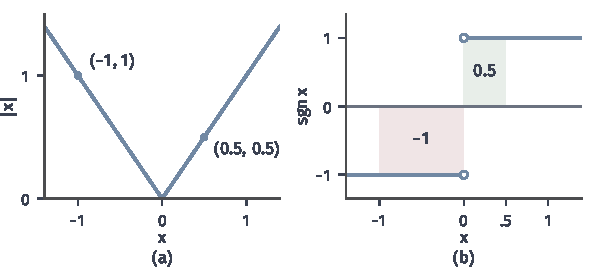
\includegraphics[width=100mm]{figures/04-spaces-measures-and-geometry/02-measure/matplotlib/weakd-abs-sign/figure.pdf}
  \caption{尖点函数与它的弱导数。(a)~$f(x)=\lvert x\rvert$在原点连续但有尖点，两个圆点在一维恢复公式中使用。(b)~弱导数$\operatorname{sgn}x$在原点两侧分别为$-1$与$1$，空心点表示原点的取值可以任意约定，弱导数作为等价类不受影响。填充部分是$[-1,0.5]$上的有向面积，红色部分为$-1$，绿色部分为$0.5$。}
  \label{fig:weakd-abs-sign}
\end{BookInlineFigure}

原点处的两个端点项相消，靠的是$\lvert x\rvert$在原点连续，两侧的极限值相同。下面的阶跃函数在原点断开，同样的计算会在原点留下一项。

\paragraph{跳跃}
取$H=\mathbf 1_{(0,\infty)}$。对测试函数$\varphi$，
\begin{equation}
-\int_{-\infty}^{\infty}H\,\varphi'\,\mathrm dx=-\int_0^\infty\varphi'\,\mathrm dx=\varphi(0).
\label{eq:weakd-step-derivative}
\end{equation}
用上面的$\varphi$可以核对：$\varphi(0)=1$，而
\[
-\int_0^1\varphi'\,\mathrm dx=\varphi(0)-\varphi(1)=1 .
\]

若$H$有弱导数$g$，就应有$\int g\varphi=\varphi(0)$对所有测试函数成立。$H$在原点以外处处可导且经典导数为零，但零函数不满足这个要求：$\int0\cdot\varphi=0$，而$\varphi(0)$可以不为零。不仅零函数不行，任何局部可积函数都不行。

\begin{example}[跳跃不产生局部可积的弱导数]
\label{ex:weakd-step-no-weak-derivative}
反设$g\in L^1_{\mathrm{loc}}(\mathbb R)$使$\int g\varphi=\varphi(0)$对所有测试函数成立。取测试函数
\[
\chi=\mathrm e\,\psi ,
\]
其中$\psi$为式~\eqref{eq:weakd-bump}的隆起函数，$\mathrm e$是自然常数。于是$0\leq\chi\leq1$，$\chi(0)=1$，支撑在$[-1,1]$内。对$0<\varepsilon\leq1$令$\varphi_\varepsilon(x)=\chi(x/\varepsilon)$，它支撑在$[-\varepsilon,\varepsilon]$内，$\varphi_\varepsilon(0)=1$，于是
\[
1=\varphi_\varepsilon(0)=\int g\,\varphi_\varepsilon\,\mathrm dx\leq\int_{-\varepsilon}^{\varepsilon}\lvert g\rvert\,\mathrm dx .
\]
当$\varepsilon\to0$时，$\lvert g\rvert\mathbf 1_{[-\varepsilon,\varepsilon]}$在原点以外逐点趋于零，并被可积函数$\lvert g\rvert\mathbf 1_{[-1,1]}$控制，由支配收敛定理右端趋于零，与左端的$1$矛盾。
\end{example}

例子的机制在图~\ref{fig:weakd-step-spike}(b)中：测试函数的支撑缩到原点时，读数始终是$\varphi_\varepsilon(0)=1$，而任何局部可积函数$g$的积分读数都要乘上越来越短的区间，即使$g$在原点无界，阴影面积也趋于零。跳跃把$H$的全部变化集中在一个点上，这种集中质量正是第~\ref{chap:measure}章中位于原点的单位点质量$\delta_0$。

磨光也说明了同一件事。一维时$H_\varepsilon(x)=\int_{-\infty}^x\rho_\varepsilon$，所以$H_\varepsilon'=\rho_\varepsilon$。图~\ref{fig:weakd-step-spike}(a)中这些导数越来越高越来越窄，面积保持为$1$，极限不是一个函数，而是原点上的集中质量。

\begin{BookInlineFigure}
  \centering
  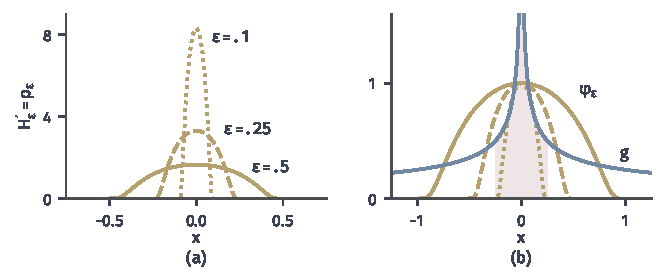
\includegraphics[width=112mm]{figures/04-spaces-measures-and-geometry/02-measure/matplotlib/weakd-step-spike/figure.pdf}
  \caption{跳跃产生集中质量。(a)~磨光后的阶跃函数的导数$H_\varepsilon'=\rho_\varepsilon$，$\varepsilon=0.5,0.25,0.1$，面积都是$1$。(b)~黄色的测试函数$\varphi_\varepsilon$，$\varepsilon=1,0.5,0.25$，在原点的值都是$1$；蓝色是局部可积函数$g(x)=0.25\lvert x\rvert^{-1/2}$，红色阴影是$\varepsilon=0.25$时的积分范围$[-\varepsilon,\varepsilon]$，随$\varepsilon\to0$面积趋于零。}
  \label{fig:weakd-step-spike}
\end{BookInlineFigure}

顺带可知，$\lvert x\rvert$没有二阶弱导数。对测试函数$\varphi$，用上一段的结果和$\operatorname{sgn}x=2H-1$，得到
\[
\int\lvert x\rvert\,\varphi''\,\mathrm dx=-\int\operatorname{sgn}(x)\,\varphi'\,\mathrm dx=2\varphi(0).
\]
要有局部可积的$g$使其等于$\int g\varphi$，同样会与上面的例子矛盾。

\paragraph{分布导数}
两个例子都可以用同一种对象描述。对任意$f\in L^1_{\mathrm{loc}}(\Omega)$与多重指标$\alpha$，规则
\begin{equation}
\varphi\longmapsto(-1)^{\lvert\alpha\rvert}\int_\Omega f\,\partial^\alpha\varphi\,\mathrm dx ,\qquad\varphi\in C_c^\infty(\Omega),
\label{eq:weakd-distributional-derivative}
\end{equation}
把每个测试函数送到一个数，并且对$\varphi$是线性的。由于$\partial^\alpha\varphi$仍是测试函数，式~\eqref{eq:weakd-local-pairing}保证这个数总是有限的。我们把这条线性规则称为$f$的$\alpha$阶\term{分布导数}（distributional derivative）。

有限维的类比是：一个线性泛函总可以写成与某个向量的内积，于是“泛函”和“向量”几乎不用区分。这里的情形不同。分布导数对每个局部可积函数都存在，但这条规则未必能写成与某个局部可积函数的积分；能写成时，那个函数就是弱导数。表~\ref{tab:weakd-distribution-examples}列出前面的例子。

\begin{BookInlineTable}
  \centering
  \begin{tabular}{@{}lll@{}}
    \toprule
    函数 & 分布导数（规则） & 弱导数\\
    \midrule
    $\lvert x\rvert$ & $\varphi\mapsto\int\operatorname{sgn}(x)\,\varphi\,\mathrm dx$ & $\operatorname{sgn}x$\\
    $\operatorname{sgn}x$ & $\varphi\mapsto2\varphi(0)$ & 不存在\\
    $H$ & $\varphi\mapsto\varphi(0)$ & 不存在\\
    \bottomrule
  \end{tabular}
  \caption{一阶分布导数与弱导数。}
  \label{tab:weakd-distribution-examples}
\end{BookInlineTable}

由测试函数判别，能这样表示时$g$几乎处处唯一，所以弱导数就是“能由局部可积函数表示的分布导数”。这类线性规则本身是广义函数理论的研究对象，点质量、读取导数值的规则$\varphi\mapsto-\varphi'(0)$都属于其中；本章只在式~\eqref{eq:weakd-distributional-derivative}的意义下使用分布导数，用它说明弱导数在什么时候不存在。

\subsection{一维弱导数与绝对连续性}
\label{sec:weakd-one-dimension}

$\lvert x\rvert$与阶跃函数的差别还有另一种说法：$\lvert x\rvert$可以由它的导数积分恢复。在图~\ref{fig:weakd-abs-sign}中取两点$x=-1$，$y=0.5$，算出两边：
\[
\lvert y\rvert-\lvert x\rvert=0.5-1=-0.5,\qquad
\int_{-1}^{0.5}\operatorname{sgn}t\,\mathrm dt=-1+0.5=-0.5 .
\]
阶跃函数的经典导数几乎处处为零，积分恒为零，恢复不了原点的跳跃。

第~\ref{chap:integration}章已经证明，有界闭区间上能由可积导数积分恢复的函数恰好是绝对连续函数。本小节证明，在一维情形，“有可积的弱导数”与“有绝对连续代表”是同一件事。下面在有界开区间$(a,b)$上工作，先处理最简单的情形：弱导数为零的函数。

\begin{lemma}[弱导数为零的函数]
\label{lem:weakd-zero-derivative}
设$f\in L^1_{\mathrm{loc}}(a,b)$，且$\int_a^bf\varphi'\,\mathrm dx=0$对所有$\varphi\in C_c^\infty(a,b)$成立。则存在常数$c$，使$f=c$几乎处处。
\end{lemma}

\begin{proof}
先看哪些测试函数是另一个测试函数的导数。设$\psi\in C_c^\infty(a,b)$且$\int_a^b\psi=0$，令
\[
\varphi(x)=\int_a^x\psi(t)\,\mathrm dt .
\]
$\varphi$光滑，$\varphi'=\psi$。在$\operatorname{supp}\psi$左侧$\varphi=0$，在其右侧$\varphi=\int_a^b\psi=0$，所以$\varphi$的支撑在$\operatorname{supp}\psi$的凸包内，是$(a,b)$中的紧集，$\varphi\in C_c^\infty(a,b)$。于是假设给出：$f$与每个积分为零的测试函数相乘后积分为零。

固定一个积分为$1$的测试函数$\theta$，例如中心在区间中点、半径足够小的磨光核。任意测试函数$\psi$可以分解为
\[
\psi=\Bigl(\int_a^b\psi\,\mathrm dx\Bigr)\theta+\Bigl(\psi-\Bigl(\int_a^b\psi\,\mathrm dx\Bigr)\theta\Bigr),
\]
其中第二项积分为零，与$f$相乘后积分为零。

令$c=\int_a^bf\theta\,\mathrm dx$，于是
\[
\int_a^bf\psi\,\mathrm dx=c\int_a^b\psi\,\mathrm dx ,
\]
即$f-c$与所有测试函数相乘后积分为零。由定理~\ref{thm:weakd-test-criterion}，$f=c$几乎处处。
\end{proof}

证明的第一步抓住了一维的特点：积分为零正是一个测试函数能写成另一个测试函数导数的条件。图~\ref{fig:weakd-primitive}比较了两种情形：积分为零时，原函数回到零，支撑仍紧；积分不为零时，原函数停留在一个正的高度，不再是紧支撑的。所以约束$\int f\varphi'=0$只漏掉了一个方向，弱导数为零的函数只剩下一个自由度，即常数。

\begin{BookInlineFigure}
  \centering
  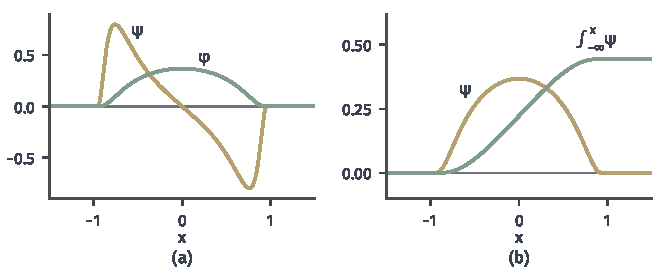
\includegraphics[width=112mm]{figures/04-spaces-measures-and-geometry/02-measure/matplotlib/weakd-primitive/figure.pdf}
  \caption{紧支撑函数的原函数。黄色为$\psi$，绿色为从左端点算起的原函数。(a)~$\psi=\varphi'$的积分为零，原函数$\varphi$回到零，支撑仍在$[-1,1]$内。(b)~$\psi$是隆起函数，积分为$c_1\approx0.444$，原函数在$x\geq1$时停留在$c_1$，不是紧支撑的。}
  \label{fig:weakd-primitive}
\end{BookInlineFigure}

有了这个引理，就可以证明一维的等价定理。

\begin{theorem}[一维弱导数与绝对连续代表]
\label{thm:weakd-absolute-continuity}
设$f,g\in L^1(a,b)$。则$g$是$f$在$(a,b)$上的弱导数，当且仅当存在$[a,b]$上的绝对连续函数$\tilde f$，满足$\tilde f=f$在$(a,b)$上几乎处处成立，并且
\begin{equation}
\tilde f(y)-\tilde f(x)=\int_x^yg(t)\,\mathrm dt ,\qquad a\leq x\leq y\leq b .
\label{eq:weakd-integral-representation}
\end{equation}
这样的$\tilde f$唯一，并且其经典导数$\tilde f'=g$几乎处处成立。
\end{theorem}

\begin{proof}
先说明变上限积分$G(x)=\int_a^xg(t)\,\mathrm dt$以$g$为弱导数。对测试函数$\varphi$，把$G$写成$\int_a^b\mathbf 1_{\{t<x\}}g(t)\,\mathrm dt$，交换积分次序，得到
\[
\begin{aligned}
\int_a^bG\,\varphi'\,\mathrm dx&=\int_a^b\!\!\int_a^b\mathbf 1_{\{t<x\}}\,g(t)\,\varphi'(x)\,\mathrm dt\,\mathrm dx\\
&=\int_a^bg(t)\Bigl(\int_t^b\varphi'(x)\,\mathrm dx\Bigr)\mathrm dt\\
&=-\int_a^bg\,\varphi\,\mathrm dt .
\end{aligned}
\]
交换次序的依据是Fubini定理：$\varphi'$有界，被积函数被$\lvert g(t)\rvert$的常数倍控制，在正方形$[a,b]^2$上可积。最后一步用了$\varphi(b)=0$。

必要性。设$g$是$f$的弱导数，则$f-G$的弱导数为零，由引理~\ref{lem:weakd-zero-derivative}，存在常数$c$使$f=c+G$几乎处处。令$\tilde f=c+G$。由第~\ref{chap:integration}章的微积分基本定理（复值时分实部、虚部），$\tilde f$在$[a,b]$上绝对连续，$\tilde f'=g$几乎处处成立，并满足式~\eqref{eq:weakd-integral-representation}。

充分性。若有满足式~\eqref{eq:weakd-integral-representation}的$\tilde f$，取$x=a$得$\tilde f=\tilde f(a)+G$。常数的弱导数为零，所以$\tilde f$以$g$为弱导数，$f=\tilde f$几乎处处，式~\eqref{eq:weakd-weak-derivative}的两边不变。

唯一性：两个连续函数若几乎处处相等，则在每点相等，因为不相等的点构成开集，而非空开区间的测度为正。
\end{proof}

定理中的端点值属于选定的代表。$f$作为几乎处处等价类没有“在$a$处的值”；正是弱导数的存在，在等价类中选出了唯一一个连续成员$\tilde f$，它在闭区间$[a,b]$上处处有值，包括两个端点。在高维情形，函数及其全部一阶弱导数可积并不保证存在连续代表，这是第~\ref{chap:sobolev-spaces}章嵌入定理研究的问题。

若只假设$f,g\in L^1_{\mathrm{loc}}(a,b)$，结论变为局部的。对每个紧区间$[c,d]\subset(a,b)$，$(c,d)$上的测试函数补零后是$(a,b)$上的测试函数，所以$g$仍是$f$在$(c,d)$上的弱导数，把定理用于$(c,d)$，得到$[c,d]$上的绝对连续代表。这些代表在区间重叠处一致，拼起来是$(a,b)$上的连续函数，在每个紧子区间上绝对连续，却未必能连续延拓到端点。

例如$(0,1)$上$f(x)=\ln x$，弱导数$1/x$局部可积而不可积，$f$在$0$附近无界。局部结论只在内部紧区间上提供积分表示，覆盖整个闭区间的结论需要$f,g$在$(a,b)$上可积。

\begin{example}[有弱导数的无界导数]
\label{ex:weakd-power}
在$(0,1)$上取$f(x)=x^{1/2}$。它是下面这个变上限积分：
\[
f(x)=\int_0^x\tfrac12\,t^{-1/2}\,\mathrm dt .
\]
被积函数可积，
\[
\int_0^1\tfrac12\,t^{-1/2}\,\mathrm dt=1 .
\]
由定理~\ref{thm:weakd-absolute-continuity}，$f$在$[0,1]$上绝对连续，弱导数是$\tfrac12x^{-1/2}$，虽然它在$0$附近无界。阶跃函数则没有绝对连续代表：在$(-1,1)$上，若$H=\mathbf 1_{(0,1)}$有连续代表，它在$(-1,0)$上恒为$0$、在$(0,1)$上恒为$1$，在原点就不可能连续，与上一小节的结论一致。
\end{example}

\subsection{磨光的求导规则}
\label{sec:weakd-mollification-derivative}

图~\ref{fig:weakd-mollifier}中，磨光后的$\lvert x\rvert$的经典导数，看上去恰好是磨光后的$\operatorname{sgn}x$。对有弱导数的函数，这个现象是一般的：先磨光再求经典导数，与先取弱导数再磨光，得到同一个函数。

\begin{theorem}[磨光与弱导数交换]
\label{thm:weakd-mollification-commute}
设$f\in L^1_{\mathrm{loc}}(\Omega)$有弱导数$\partial^\alpha f\in L^1_{\mathrm{loc}}(\Omega)$，$\varepsilon>0$。则在$\Omega_\varepsilon$上
\begin{equation}
\partial^\alpha(f_\varepsilon)=(\partial^\alpha f)_\varepsilon ,
\label{eq:weakd-mollification-commute}
\end{equation}
左端是光滑函数$f_\varepsilon$的经典导数，右端是弱导数的磨光。
\end{theorem}

\begin{proof}
固定$x\in\Omega_\varepsilon$。函数$\varphi_x(y)=\rho_\varepsilon(x-y)$是$\Omega$上的测试函数，定理~\ref{thm:weakd-test-criterion}的证明已核对其支撑。对$y$求导时，链式法则对每个坐标产生一个因子$-1$，所以
\[
\partial_y^\alpha\varphi_x(y)=(-1)^{\lvert\alpha\rvert}(\partial^\alpha\rho_\varepsilon)(x-y).
\]

由定理~\ref{thm:weakd-mollification-smooth}的式~\eqref{eq:weakd-mollifier-derivative}与上式，得到
\[
\begin{aligned}
\partial^\alpha f_\varepsilon(x)&=\int_\Omega(\partial^\alpha\rho_\varepsilon)(x-y)\,f(y)\,\mathrm dy\\
&=(-1)^{\lvert\alpha\rvert}\int_\Omega f\,\partial^\alpha\varphi_x\,\mathrm dy\\
&=\int_\Omega(\partial^\alpha f)\,\varphi_x\,\mathrm dy=(\partial^\alpha f)_\varepsilon(x),
\end{aligned}
\]
第三个等号是弱导数的定义~\eqref{eq:weakd-weak-derivative}用于测试函数$\varphi_x$。
\end{proof}

证明只用了一次弱导数的定义，测试函数恰好是平移、反射后的磨光核。定义中“对所有测试函数成立”的要求在这里被具体地用上了：每个$x$都需要一个不同的测试函数。

\paragraph{函数与导数的同时逼近}
把交换规则与上一节的局部逼近结合，磨光就能在每个内部紧集上同时逼近函数和它的弱导数。

\begin{theorem}[磨光的同时局部逼近]
\label{thm:weakd-simultaneous-approximation}
设$f\in L^1_{\mathrm{loc}}(\Omega)$，$A$是一组有限多个多重指标，对每个$\alpha\in A$，$f$都有弱导数$\partial^\alpha f\in L^1_{\mathrm{loc}}(\Omega)$。设$K\subset\Omega$紧。则$f_\varepsilon$在$K$的一个邻域上光滑，并且当$\varepsilon\to0$时
\begin{equation}
\begin{gathered}
\int_K\lvert f_\varepsilon-f\rvert\,\mathrm dx\to0,\\
\int_K\lvert\partial^\alpha f_\varepsilon-\partial^\alpha f\rvert\,\mathrm dx\to0\quad(\alpha\in A).
\end{gathered}
\label{eq:weakd-simultaneous-approximation}
\end{equation}
\end{theorem}

\begin{proof}
当$\varepsilon<\operatorname{dist}(K,\Omega^{c})$时$K\subset\Omega_\varepsilon$，由定理~\ref{thm:weakd-mollification-smooth}，$f_\varepsilon$在开集$\Omega_\varepsilon$上光滑。第一个极限是定理~\ref{thm:weakd-local-approximation}。

对$\alpha\in A$，由式~\eqref{eq:weakd-mollification-commute}，在$K$上
\[
\partial^\alpha f_\varepsilon-\partial^\alpha f=(\partial^\alpha f)_\varepsilon-\partial^\alpha f .
\]
把定理~\ref{thm:weakd-local-approximation}用于局部可积函数$\partial^\alpha f$即得。$A$有限，所有分量可以同时取充分小的$\varepsilon$。
\end{proof}

以$\lvert x\rvert$为例把两种误差算出来，取$\Omega=\mathbb R$，$K=[-1,1]$，$\varepsilon\leq0.5$。先看导数的误差。由$\operatorname{sgn}x=2H-1$和例~\ref{ex:weakd-step-mollification}的计算，
\[
\int_K\bigl\lvert(\operatorname{sgn})_\varepsilon-\operatorname{sgn}\bigr\rvert\,\mathrm dx=2\varepsilon m_1 .
\]

再看函数本身的误差。记$f(x)=\lvert x\rvert$。把$\rho_\varepsilon$的偶性用上，$A=f_\varepsilon-f$可以写成
\[
A(x)=\int_{\lvert z\rvert\leq\varepsilon}\rho_\varepsilon(z)\,\frac{\lvert x-z\rvert+\lvert x+z\rvert-2\lvert x\rvert}{2}\,\mathrm dz .
\]
由三角不等式，被积函数非负，所以$A\geq0$。

因此误差的积分就是$A$的积分。交换积分次序，并用
\[
\int_{-1}^1\bigl(\lvert x-z\rvert-\lvert x\rvert\bigr)\,\mathrm dx=z^2\qquad(\lvert z\rvert\leq1),
\]
再用替换$z=\varepsilon u$，得到
\[
\int_K\lvert f_\varepsilon-f\rvert\,\mathrm dx=\int_{\lvert z\rvert\leq\varepsilon}\rho_\varepsilon(z)\,z^2\,\mathrm dz=\varepsilon^2m_2 .
\]

表~\ref{tab:weakd-simultaneous-errors}是这两个公式的数值。函数误差按$\varepsilon^2$减小，导数误差按$\varepsilon$减小：弱导数在原点有跳跃，比函数本身更难逼近。

\begin{BookInlineTable}
  \centering
  \begin{tabular}{@{}lll@{}}
    \toprule
    $\varepsilon$ & 函数误差$\varepsilon^2m_2$ & 导数误差$2\varepsilon m_1$\\
    \midrule
    $0.5$ & $0.0395$ & $0.3345$\\
    $0.25$ & $0.0099$ & $0.1672$\\
    $0.1$ & $0.0016$ & $0.0669$\\
    \bottomrule
  \end{tabular}
  \caption{$\lvert x\rvert$的同时逼近误差，$K=[-1,1]$，$m_1\approx0.3345$，$m_2\approx0.1581$。}
  \label{tab:weakd-simultaneous-errors}
\end{BookInlineTable}

阶跃函数$H$的情形不同。$H_\varepsilon$也是光滑函数，它的导数$H_\varepsilon'=\rho_\varepsilon$却不在积分意义下收敛：对任意$\delta>0$，只要$\varepsilon<\delta$，$\rho_\varepsilon$在$\lvert x\rvert\geq\delta$上恒为零，所以极限若是某个函数，只能是零函数；而$\int\rho_\varepsilon=1$并不趋于零。这与$H$没有弱导数相符。

定理~\ref{thm:weakd-simultaneous-approximation}给出的是局部的积分逼近：逼近函数只在离边界大于$\varepsilon$的地方有定义，误差用积分衡量。把这些局部逼近拼成整个区域上的光滑逼近，并在$L^p$范数下控制函数与弱导数的误差，是第~\ref{chap:sobolev-spaces}章光滑稠密性定理的任务。

\section{本章小结}
\label{sec:weakd-summary}

本章开头问：对只在几乎处处意义下确定、可能有尖点或跳跃的函数，能否用光滑函数逼近，能否给它一个可以运算的导数。第一个问题由局部平均回答。局部可积只要求函数在每个紧含于区域的集合上可积，这恰好使它与测试函数的乘积可以积分。以归一化的隆起函数为权重做局部平均，得到磨光函数；它的光滑性完全来自核，因为对参数求导可以全部移到核上，而局部可积的函数提供与参数无关的可积上界。

磨光函数逼近原函数的依据是平移的积分连续性。从外测度的矩形覆盖得到开集外逼近与紧集内逼近，再用矩形的有限并和简单函数逼近可积函数，就能证明小平移只引起小的积分误差。核非负且积分为$1$，使磨光误差成为平移误差的加权平均，所以在每个内部紧集上$\int_K\lvert f_\varepsilon-f\rvert\to0$。这种逼近只控制积分误差，阶跃函数的例子说明逐点最大误差可以不趋于零。由于磨光值本身就是一个测试积分，局部逼近立即给出测试函数判别：与全部测试函数积分为零的局部可积函数几乎处处为零。

第二个问题由测试恒等式回答。光滑函数的分部积分把导数转到测试函数上，测试函数的紧支撑使边界项消失，得到的右端只要求函数局部可积。弱导数就是能代替经典导数放进这个恒等式的局部可积函数；测试函数判别保证它几乎处处唯一，对光滑函数它与经典导数一致。

尖点与跳跃的对照说明了定义的边界：$\lvert x\rvert$在原点两侧的端点项相消，弱导数是$\operatorname{sgn}x$；阶跃函数留下读取原点值的规则，它是分布导数，却不能由任何局部可积函数表示。分布导数对每个局部可积函数都存在，弱导数还要求这条线性规则由局部可积函数给出。

在一维有界区间上，函数及其弱导数可积，等价于函数有绝对连续代表并能由弱导数积分恢复；弱导数为零的函数是常数，这一点依靠积分为零的测试函数恰好是测试函数的导数。端点值属于唯一的连续代表，局部可积的情形只在内部紧区间上得到绝对连续代表。最后，磨光与弱导数可以交换次序，因此在每个内部紧集上，光滑的磨光函数及其经典导数同时在积分意义下逼近原函数及其弱导数。

这些结论都是局部的，并且用积分误差衡量。把函数与若干阶弱导数的$L^p$大小合成范数，研究空间的完备性、整个区域上的光滑稠密性、边界处理与嵌入，是第~\ref{chap:sobolev-spaces}章的内容；磨光在$L^p$范数下的收敛由第~\ref{chap:function-approximation}章处理。下一章回到测度本身，研究一个测度何时能写成另一个测度的加权积分。


\chapter{测度的密度}
\label{chap:measure-densities}
\label{chap:densities-change-of-measure}

区间$[0,1]$上的质量可以均匀分布，也可以向右端堆积，还可以有一部分集中在一个点上。用长度作参照，均匀分布的质量处处是长度的同一个倍数，向右堆积的质量在右端是长度的更大倍数，而点上的质量无论乘以什么倍数都不能从长度得到，因为单点的长度为零。本章研究这种“相对于参考测度的倍数”：一个测度何时能写成另一个测度的加权积分，权重函数怎样计算，以及有了权重之后积分怎样改写。

回答从测度之间最粗的关系开始。第一节只看零测集：参考测度认为可以忽略的集合，目标测度是否也忽略；两个测度能否被一个可测集合完全分开。第二节先从“给定权重得到测度”的方向定义相对密度，再用Radon–Nikodym定理说明，在$\sigma$有限条件下绝对连续恰好保证密度存在，并且密度几乎处处唯一。第三节把一般的测度分成能用密度表示的部分与和参考测度相互奇异的部分，并在实轴上把后者进一步分成点质量与奇异连续质量。

有了密度，第四节建立运算规则：换测度公式把对目标测度的积分改写成对参考测度的加权积分，相对同一参考的密度可以线性组合，逐次更换参考时密度相乘，两个测度等价时密度可以取倒数。第五节回到具体对象，由点质量之比计算离散测度的密度，由累积函数的导数计算实轴测度的密度，并说明导数为何不能恢复点质量与奇异连续质量。

本章的测度都定义在同一个可测空间上，所用的测度构造、有符号测度的Hahn与Jordan分解来自第~\ref{chap:measure}章，积分、单调收敛定理与绝对连续函数的微积分基本定理来自第~\ref{chap:integration}章。点经过映射从一个空间移到另一个空间时质量怎样转移，以及相应的坐标换元，是第~\ref{chap:pushforward-measures}章的内容。

\section{绝对连续与相互奇异}
\label{sec:dens-ac-singular}

同一个可测空间上可以放很多测度：长度、点质量、计数测度以及它们的加权和。比较两个测度时，最粗也最基本的信息是它们怎样对待“可以忽略的集合”。本节固定可测空间$(X,\mathcal A)$上的两个非负测度，一个作为参考，一个作为要描述的目标，只用集合上的测度值回答两个问题：参考测度忽略的集合，目标测度是否也忽略；两个测度的质量能否分别集中在两个互不相交的可测集合上。这两种关系都由集合定义，不涉及积分，也还没有任何密度函数。

记号约定：$\lambda$表示实轴上的Lebesgue测度；对可测集$E$，$\lambda|_E(A)=\lambda(A\cap E)$表示把$\lambda$限制到$E$上得到的测度，它仍定义在整条实轴上；$\delta_a$表示位于点$a$的单位点质量，$\delta_a(A)=1$当且仅当$a\in A$。

\subsection{测度的绝对连续}
\label{sec:dens-absolute-continuity}

设$\mu$是我们用来判断“哪些集合可以忽略”的参考测度。若凡是$\mu$忽略的集合，目标测度$\nu$也一律忽略，那么在$\mu$下几乎处处成立的结论，在$\nu$下也几乎处处成立。下一节会看到，这正是用$\mu$的加权积分表示$\nu$的前提。

\begin{definition}[测度的绝对连续与等价]
\label{def:dens-absolute-continuity}
设$\mu,\nu$是$(X,\mathcal A)$上的非负测度。若对每个$A\in\mathcal A$，
\[
\mu(A)=0\ \Longrightarrow\ \nu(A)=0 ,
\]
就称$\nu$相对于$\mu$\term{绝对连续}（absolutely continuous），记作$\nu\ll\mu$。若$\nu\ll\mu$与$\mu\ll\nu$同时成立，就称$\mu$与$\nu$是\term{等价测度}（equivalent measures），记作$\mu\sim\nu$。
\end{definition}

关系有方向。$\nu\ll\mu$说的是$\mu$的零测集族包含在$\nu$的零测集族之中，参考测度写在右边。它只比较测度值是否为零，不比较非零值的大小；等价也只说明两个测度认可同一族零测集，不说明它们给同一集合相同的值。

\begin{example}[两点空间上的单向关系]
\label{ex:dens-two-point}
取$X=\{0,1\}$，$\mathcal A$为全部子集，$\mu=\delta_0+\delta_1$，$\nu=\delta_0$。$\mu$给每个单点质量$1$，零测集只有空集，所以条件“$\mu(A)=0\Rightarrow\nu(A)=0$”只需对$A=\varnothing$检查，$\nu\ll\mu$成立。反方向不成立：$\nu(\{1\})=0$，而$\mu(\{1\})=1$。再取$\rho=2\delta_0+5\delta_1$，它与$\mu$的零测集都只有空集，于是$\rho\sim\mu$，尽管$\rho(\{1\})=5\neq\mu(\{1\})$。
\end{example}

参考测度不必是Lebesgue测度。上例中参考测度是离散的，零测集由“哪些点没有质量”决定。在实轴上以$\lambda$为参考时，零测集包含所有单点和可数集，因此容易只拿单点来检验。单点检查足以否定$\delta_0\ll\lambda$：$\lambda(\{0\})=0$，而$\delta_0(\{0\})=1$。但单点检查一般不够。

\begin{example}[区间上的连续质量]
\label{ex:dens-two-intervals}
比较$\lambda|_{[0,1]}$与$\lambda|_{[2,3]}$。两者给每个单点的质量都是零，单点完全看不出差别；然而$\lambda|_{[2,3]}([0,1])=0$，$\lambda|_{[0,1]}([0,1])=1$，所以$\lambda|_{[0,1]}\ll\lambda|_{[2,3]}$不成立，反方向同理。另一方面$\lambda|_{[0,1]}\ll\lambda$：$\lambda(A)=0$推出$\lambda(A\cap[0,1])=0$。原因在于$[0,1]$不可数，可数可加性不允许把它的质量拆成单点质量之和；定义要求对每个可测集检查。图~\ref{fig:dens-absolute-continuity}对照了本例与上一例。
\end{example}

\begin{figure}[!htbp]
  \centering
  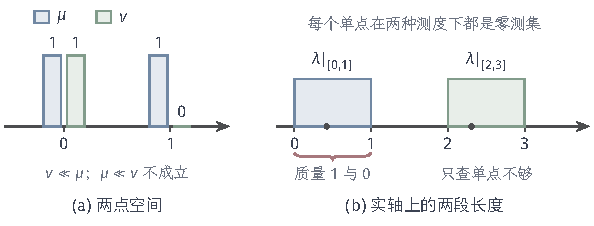
\includegraphics[width=100.669mm]{figures/02-abstract-mathematics/01-metric-and-measure/tikz/c2-absolute-continuity/figure.pdf}
  \caption{绝对连续比较的是零测集。(a)两点空间上$\mu=\delta_0+\delta_1$（蓝）与$\nu=\delta_0$（绿）：$\mu$只把空集看作零测集，所以$\nu\ll\mu$；$\nu$在点$1$的质量为零而$\mu$不为零，所以反向不成立。(b)$\lambda|_{[0,1]}$（蓝）与$\lambda|_{[2,3]}$（绿）在每个单点上都为零，但在$[0,1]$上分别为$1$与$0$，两者互不绝对连续。}
  \label{fig:dens-absolute-continuity}
\end{figure}

\paragraph{与函数的绝对连续}
名称“绝对连续”在第~\ref{chap:integration}章已经用于函数：区间上的函数若在总长度很小的有限个小区间上增量之和也很小，就称它绝对连续。两个概念分别定义，联系要等到第~\ref{sec:dens-cumulative-density}小节才说明：单调函数绝对连续，当且仅当它的增量所产生的测度相对于$\lambda$绝对连续。测度的名称也与“小推出小”有关：若$\nu$有限，则$\nu\ll\mu$等价于对每个$\varepsilon>0$存在$\delta>0$，使$\mu(A)<\delta$推出$\nu(A)<\varepsilon$。本章不使用这一刻画，这里不给出证明。

\subsection{测度的相互奇异}
\label{sec:dens-mutual-singularity}

绝对连续描述的是“参考测度忽略的地方，目标测度也忽略”。与它相对的另一种极端是两个测度各自待在对方忽略的区域里，质量完全不重叠。若$\nu(X\setminus N)=0$，就说$\nu$\emph{集中}在可测集$N$上。

\begin{definition}[相互奇异]
\label{def:dens-mutual-singularity}
设$\mu,\nu$是$(X,\mathcal A)$上的非负测度。若存在$N\in\mathcal A$，使
\[
\mu(N)=0,\qquad\nu(X\setminus N)=0 ,
\]
就称$\mu$与$\nu$\term{相互奇异}（mutually singular），记作$\mu\perp\nu$。
\end{definition}

定义对两个测度是对称的：令$N'=X\setminus N$，则$\nu(N')=0$且$\mu(X\setminus N')=0$，同一关系从$\nu$的角度看就是用补集作分割。直观地说，$X$被一个可测集合分成两块，$\nu$的全部质量在$N$中，$\mu$的全部质量在$X\setminus N$中。在实轴上取$\mu=\lambda|_{[0,1]}$，$\nu=\tfrac12\delta_{1/2}$，$N=\{1/2\}$，则$\mu(N)=0$，$\nu(\mathbb R\setminus N)=0$，所以$\mu\perp\nu$。点$1/2$位于区间内部，相互奇异并不要求两种质量在位置上分开。

两种关系检查的是不同的事。$\nu\ll\mu$问的是$\mu$零测集上有没有$\nu$质量；$\nu\perp\mu$问的是$\nu$能否全部放进一个$\mu$零测集。二者几乎不能同时成立：若$\nu\ll\mu$且$\nu\perp\mu$，取定义中的$N$，则$\mu(N)=0$推出$\nu(N)=0$，又$\nu(X\setminus N)=0$，所以$\nu(X)=0$，$\nu$是零测度。一般的测度两种关系都不满足，例如$\lambda|_{[0,1]}+\delta_2$相对于$\lambda$，第~\ref{sec:dens-decomposition}节将把它拆成满足两种关系的两部分。

\paragraph{集中集合与闭支撑}
在实轴或$\mathbb R^d$上，“相互奇异”很容易被想象成两团质量隔着一段距离。为了说明这种想象不对，先定义Borel测度$\mu$的\term{闭支撑}（support of a measure）：它是这样一些点$x$的集合，$x$的每个开邻域都有正的$\mu$质量。闭支撑的补集是所有$\mu$零测开集之并，因而闭支撑是闭集。$\lambda|_{[0,1]}$的闭支撑是$[0,1]$，$\delta_{1/2}$的闭支撑是$\{1/2\}$，两者相交，测度却相互奇异。

\begin{example}[闭支撑相同而相互奇异]
\label{ex:dens-rationals}
设$(q_n)_{n\geq1}$列举全部有理数，令
\[
\mu=\sum_{n=1}^\infty2^{-n}\delta_{q_n},\qquad\nu=\sum_{n=1}^\infty2^{-n}\delta_{q_n+\sqrt2},
\]
两者都是总质量为$1$的有限测度。$\mu$集中在$\mathbb Q$上，$\nu$集中在$\mathbb Q+\sqrt2$上。这两个集合不相交：若$q=q'+\sqrt2$，则$\sqrt2=q-q'$是有理数，矛盾。取$N=\mathbb Q+\sqrt2$，有$\mu(N)=0$，$\nu(\mathbb R\setminus N)=0$，所以$\mu\perp\nu$。

另一方面，$\mathbb Q$与$\mathbb Q+\sqrt2$都在实轴上稠密，每个非空开区间中两者都有点，所以两个测度在每个非空开区间上都有正质量，闭支撑都是整条实轴。图~\ref{fig:dens-mutually-singular}画出了两组点中的前几个，它们彼此交错。
\end{example}

\begin{figure}[!htbp]
  \centering
  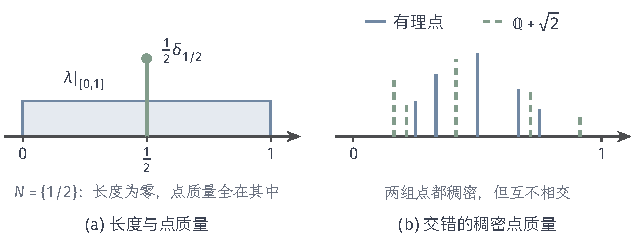
\includegraphics[width=107.668mm]{figures/02-abstract-mathematics/01-metric-and-measure/tikz/c2-mutually-singular/figure.pdf}
  \caption{相互奇异是可测集合上的分离。(a)$\lambda|_{[0,1]}$与$\tfrac12\delta_{1/2}$相互奇异，分离集$N=\{1/2\}$位于区间内部。(b)$\mu=\sum_n2^{-n}\delta_{q_n}$集中在有理点上（蓝色实线），$\nu=\sum_n2^{-n}\delta_{q_n+\sqrt2}$集中在$\mathbb Q+\sqrt2$上（绿色虚线）；图中只画出$[0,1]$内各几个点，线高仅示意权重递减。两组点在每个开区间中都出现，但互不相交，所以$\mu\perp\nu$。}
  \label{fig:dens-mutually-singular}
\end{figure}

这个例子说明，判断相互奇异要找可测的集中集合，而不是看闭支撑是否相交。反方向的蕴含是成立的：若两个闭支撑不相交，取$N$为$\nu$的闭支撑，则$\nu(X\setminus N)=0$：闭支撑的补集中每点都落在某个中心与半径均为有理数、且含于一个$\nu$零测开集的球内，这样的球只有可数个，所以补集是可数个$\nu$零测集之并，而$N$落在$\mu$闭支撑的补集中，$\mu(N)=0$。所以闭支撑不交是相互奇异的充分条件，不是必要条件。顺带一提，上例中的$\mu,\nu$都集中在可数集上，因而都与$\lambda$相互奇异。

\section{相对密度}
\label{sec:dens-relative-density}

绝对连续只是一个关于零测集的条件，它没有给出任何函数。本节从相反的方向进入：先给定参考测度和一个非负权重，用积分产生一个新测度，并把权重称为新测度的相对密度，这一方向不需要任何条件。然后问，给定两个测度，能否找到这样的权重。Radon–Nikodym定理回答，在$\sigma$有限的条件下，绝对连续恰好是所需的条件，而且权重在参考测度几乎处处的意义下唯一。

\subsection{由密度生成测度}
\label{sec:dens-weighted-measure}

给定参考测度，怎样用一个权重函数得到新测度？先在有限点集上看清乘数的含义，再用积分把它推广到一般测度，最后说明权重只在几乎处处意义下确定。

\paragraph{有限点集上的质量之比}
设$X=\{a,b,c\}$，目标测度$\nu$给三个点的质量写成向量是$(0.2,0.5,0.3)$。若参考测度是计数测度，每点质量为$1$，从参考质量得到目标质量只需在每点乘以$0.2,0.5,0.3$。若参考测度改为$\mu'=2\delta_a+\delta_b+\delta_c$，点$a$的乘数就要改成$0.2/2=0.1$，另外两点不变。

把乘数写成对角矩阵，这个关系就是矩阵乘向量。对参考$\mu'$，
\[
\begin{pmatrix}0.2\\0.5\\0.3\end{pmatrix}
=\begin{pmatrix}0.1&&\\&0.5&\\&&0.3\end{pmatrix}
\begin{pmatrix}2\\1\\1\end{pmatrix}.
\]
任一子集的目标质量都等于参考质量乘以乘数后求和，例如
\[
\nu(\{a,b\})=0.1\cdot2+0.5\cdot1=0.7 .
\]

图~\ref{fig:dens-mass-ratio}并排画出这两种参考。目标测度在两栏中完全相同，变化的只有参考质量，乘数随之改变。所以乘数描述的是“目标相对于参考”的换算比例，离开参考测度谈乘数没有意义。

\begin{BookInlineFigure}
  \centering
  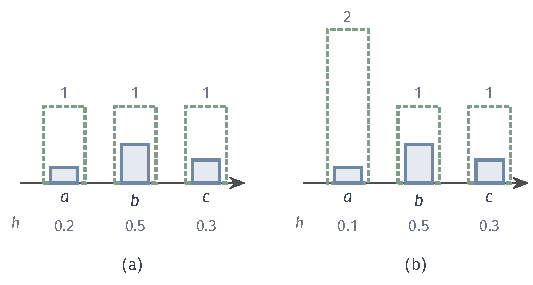
\includegraphics[width=90.255mm]{figures/04-spaces-measures-and-geometry/02-measure/tikz/dens-mass-ratio/figure.pdf}
  \caption{密度是目标质量与参考质量之比。三点集$\{a,b,c\}$上的目标质量$(0.2,0.5,0.3)$（蓝色实心柱）保持不变。(a)参考为计数测度（绿色虚线框高为$1$），每点的密度$h$等于目标质量本身；(b)参考权重改为$(2,1,1)$，点$a$的密度变为$0.2/2=0.1$，其余两点不变。}
  \label{fig:dens-mass-ratio}
\end{BookInlineFigure}

在实轴的长度测度下，每个单点的长度都是$0$，“单点质量相除”变成$0/0$，一般情形不能逐点定义比值，对角矩阵的类比在这里失效。可以保留的是另一半：在每个集合上，参考质量乘以权重再累计，应当得到目标质量。在有限点集上累计是求和，一般情形下就是第~\ref{chap:integration}章的积分。下面约定
\[
\int_Ah\,\mathrm d\mu=\int_Xh\mathbf 1_A\,\mathrm d\mu .
\]

\paragraph{加权测度}
先说明“给定权重，产生测度”总是可行的。这一方向相当于用对角矩阵去乘向量，不需要任何条件。

\begin{theorem}[加权测度]
\label{thm:dens-weighted-measure}
设$(X,\mathcal A,\mu)$是测度空间，$h:X\to[0,+\infty]$可测。令
\begin{equation}
\nu_h(A)=\int_Ah\,\mathrm d\mu ,\qquad A\in\mathcal A .
\label{eq:dens-weighted}
\end{equation}
则$\nu_h$是$(X,\mathcal A)$上的非负测度，并且$\nu_h\ll\mu$。
\end{theorem}

\begin{proof}
空集上的被积函数恒为零，所以$\nu_h(\varnothing)=0$，且$\nu_h$取值于$[0,+\infty]$。

设$A_1,A_2,\ldots\in\mathcal A$两两不交，$A=\bigcup_nA_n$。各$A_n$不交，所以逐点有
\[
h\mathbf 1_A=\sum_{n\geq1}h\mathbf 1_{A_n} .
\]
部分和是递增的非负可测函数列，由单调收敛定理可以逐项积分，得到
\[
\nu_h(A)=\int_Xh\mathbf 1_A\,\mathrm d\mu=\sum_{n=1}^\infty\int_Xh\mathbf 1_{A_n}\,\mathrm d\mu=\sum_{n=1}^\infty\nu_h(A_n).
\]
所以$\nu_h$可数可加。

若$\mu(A)=0$，函数$h\mathbf 1_A$在$\mu$零测集之外为零，其积分为$0$，故$\nu_h(A)=0$，即$\nu_h\ll\mu$。
\end{proof}

证明只用了单调收敛定理，没有要求$\mu$或$h$有限。若$h$在一个正测度集合上取$+\infty$，$\nu_h$可能连$\sigma$有限都不是，但它仍是测度。定理的最后一句说明：凡是能由参考测度加权得到的测度，都相对于参考测度绝对连续。

\begin{definition}[相对密度]
\label{def:dens-relative-density}
设$\mu,\nu$是$(X,\mathcal A)$上的非负测度。若可测函数$h:X\to[0,+\infty]$满足
\begin{equation}
\nu(A)=\int_Ah\,\mathrm d\mu ,\qquad A\in\mathcal A ,
\label{eq:dens-definition}
\end{equation}
就称$h$是$\nu$相对于$\mu$的一个\term{相对密度}（relative density），也称\term{Radon–Nikodym密度}（Radon-Nikodym derivative），记作$\dfrac{\mathrm d\nu}{\mathrm d\mu}=h$；$\mu$称为\term{参考测度}（reference measure）。
\end{definition}

密度的数值同时依赖目标测度与参考测度：上面的三点例子中，同一个$\nu$换一个参考，点$a$的密度就从$0.2$变为$0.1$。记号$\mathrm d\nu/\mathrm d\mu$借用了导数的写法，但它不是对某个坐标求导，而是两种测度之间的换算权重。由定理~\ref{thm:dens-weighted-measure}，密度存在的一个必要条件是$\nu\ll\mu$。

\paragraph{几乎处处版本}
定义说的是“一个”密度。若$h=g$在$\mu$几乎处处成立，则对每个$A$，$h\mathbf 1_A$与$g\mathbf 1_A$也$\mu$几乎处处相等，积分相同，所以$h,g$生成同一个测度。在$[0,1]$上，$h=1$与$g=1+\mathbf 1_{\mathbb Q\cap[0,1]}$都给出$\lambda|_{[0,1]}$，因为二者只在可数集上不同。

因此记号$\mathrm d\nu/\mathrm d\mu$只指其中任一个版本，关于密度的逐点断言，如“$h>0$”“$h<\infty$”，都只在$\mu$几乎处处的意义下才有意义。这与有限点集上不同：在每点都有正质量时，比值逐点确定；在长度下，单点不承载质量，所以单点上的值不算数。

\begin{example}[分段常值密度]
\label{ex:dens-piecewise}
在$[0,1]$上取$\mu=\lambda|_{[0,1]}$，并令
\[
h=\tfrac32\mathbf 1_{[0,1/2)}+\tfrac12\mathbf 1_{[1/2,1]} .
\]
由简单函数的积分，在每一块上把参考质量乘以该块的系数再相加：
\[
\nu_h(E)=\tfrac32\lambda\bigl(E\cap[0,\tfrac12)\bigr)+\tfrac12\lambda\bigl(E\cap[\tfrac12,1]\bigr).
\]
取$E=[0,1]$，得到
\[
\nu_h([0,1])=\tfrac32\cdot\tfrac12+\tfrac12\cdot\tfrac12=\tfrac34+\tfrac14=1 ,
\]
所以$\nu_h$是概率测度。对$E=[1/4,3/4]$，两块的长度各为$\tfrac14$，于是
\[
\nu_h(E)=\tfrac32\cdot\tfrac14+\tfrac12\cdot\tfrac14=\tfrac38+\tfrac18=\tfrac12 .
\]
\end{example}

图~\ref{fig:dens-weighted-measure}(a)中，$E$的质量$\tfrac12$就是$E$上方、密度图像之下的面积。(b)说明在零测点上改动密度不改变面积，这是“几乎处处版本”的几何含义。

\begin{BookInlineFigure}
  \centering
  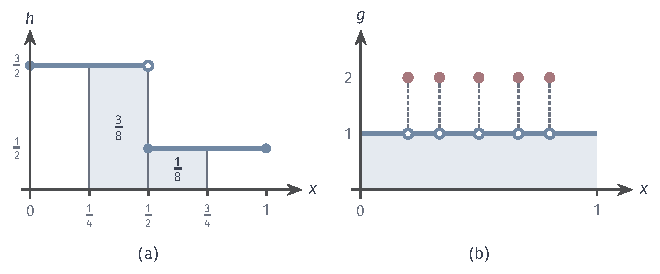
\includegraphics[width=111.693mm]{figures/04-spaces-measures-and-geometry/02-measure/tikz/dens-weighted-measure/figure.pdf}
  \caption{由密度构造测度，以及几乎处处版本。(a)参考测度为$[0,1]$上的长度，密度$h$在$[0,1/2)$上取$3/2$、在$[1/2,1]$上取$1/2$；集合$A=[1/4,3/4]$的质量$\nu_h(A)$是$A$上方的阴影面积$3/8+1/8=1/2$。(b)常数密度$1$与在若干零测点（红点，示意有理点）上改取$2$的函数$g$给出同一测度，因为改动的位置不承载长度。}
  \label{fig:dens-weighted-measure}
\end{BookInlineFigure}

概率论中的概率质量函数与概率密度函数都是这一定义的特例，区别只在参考测度：前者相对于可数集上的计数测度，后者相对于Lebesgue测度，可参考\BookChapterRef{chap:random-variables}{卷七第2章“随机变量的分布”}。一般的密度不要求总积分为一，$\int_Xh\,\mathrm d\mu=\nu(X)$只在目标是概率测度时等于$1$。

概率密度在某点的值也可以大于$1$，上例中$h$在$[0,1/2)$上就等于$\tfrac32$。密度值不是该点的概率，只有在集合上积分后才成为质量。

\subsection{Radon–Nikodym定理}
\label{sec:dens-radon-nikodym}

现在反过来：给定两个测度，能否找到同一个函数$h$，使式~\eqref{eq:dens-definition}对所有可测集同时成立？$\nu\ll\mu$是必要条件。它是否充分是一个真正的问题，因为要同时满足的等式有不可数多个，而绝对连续只告诉我们零测集的信息。

在有限点集上答案是直接的：$\nu\ll\mu$表示$m_i=0$时$p_i=0$，所以在$m_i>0$处令$h_i=p_i/m_i$，在$m_i=0$处任取一个值，就得到密度。一般情形没有逐点比值可用，下面的定理用一种优化的办法把比值“求”出来。

\begin{theorem}[Radon–Nikodym定理]
\label{thm:dens-radon-nikodym}
设$\mu,\nu$是$(X,\mathcal A)$上的$\sigma$有限非负测度，且$\nu\ll\mu$。则存在可测函数$h:X\to[0,+\infty)$，使
\begin{equation}
\nu(A)=\int_Ah\,\mathrm d\mu ,\qquad A\in\mathcal A .
\label{eq:dens-rn}
\end{equation}
若可测函数$g:X\to[0,+\infty]$也满足这一等式，则$g=h$在$\mu$几乎处处成立。
\end{theorem}

把\term{Radon–Nikodym定理}（Radon-Nikodym theorem）与定理~\ref{thm:dens-weighted-measure}对照：那里从$h$得到测度，这里从测度得到$h$。在$\sigma$有限范围内，“$\nu$相对于$\mu$有密度”与“$\nu\ll\mu$”是同一件事。证明先处理两个测度都有限的情形，再用$\sigma$有限性把空间切成可数个有限块。

\paragraph{有限情形：取最大的候选权重}
思路是在所有“处处不超过$\nu$”的权重中找一个积分最大的。把权重想成一层一层往上堆的沙子：每个集合上堆出的量都不能超过$\nu$在该集合上的质量。若某个权重已经堆到不能再高，那么它在每个集合上就应该恰好等于$\nu$。

\begin{lemma}[有限测度的密度存在]
\label{lem:dens-rn-finite}
设$\mu,\nu$是$(X,\mathcal A)$上的有限非负测度，且$\nu\ll\mu$。则存在可测函数$h:X\to[0,+\infty)$，使
\begin{equation}
\nu(A)=\int_Ah\,\mathrm d\mu ,\qquad A\in\mathcal A .
\label{eq:dens-rn-finite}
\end{equation}
\end{lemma}

\begin{proof}
第一步，证明候选权重对取最大值封闭。令
\[
\mathcal G=\Bigl\{g:X\to[0,+\infty]\text{可测}:\ \int_Ag\,\mathrm d\mu\leq\nu(A)\ \ \forall A\in\mathcal A\Bigr\}.
\]
零函数属于$\mathcal G$。设$g_1,g_2\in\mathcal G$，$g=\max(g_1,g_2)$。对任意$A$，令
\[
A_1=A\cap\{g_1\geq g_2\},\qquad A_2=A\cap\{g_1<g_2\}.
\]
二者可测、不交且并为$A$，于是
\[
\begin{aligned}
\int_Ag\,\mathrm d\mu&=\int_{A_1}g_1\,\mathrm d\mu+\int_{A_2}g_2\,\mathrm d\mu\\
&\leq\nu(A_1)+\nu(A_2)=\nu(A),
\end{aligned}
\]
故$g\in\mathcal G$。归纳可知有限个候选的最大值仍是候选。

第二步，用单调序列达到上确界。令
\[
s=\sup_{g\in\mathcal G}\int_Xg\,\mathrm d\mu\leq\nu(X)<\infty .
\]
取$g_n\in\mathcal G$使$\int_Xg_n\,\mathrm d\mu\to s$，再令$h_n=\max(g_1,\ldots,g_n)\in\mathcal G$。$h_n$递增，且
\[
\int_Xg_n\,\mathrm d\mu\leq\int_Xh_n\,\mathrm d\mu\leq s .
\]
令$h=\lim_nh_n$。由单调收敛定理，对每个$A$，
\[
\int_Ah\,\mathrm d\mu=\lim_{n\to\infty}\int_Ah_n\,\mathrm d\mu\leq\nu(A),
\]
所以$h\in\mathcal G$，并且$\int_Xh\,\mathrm d\mu=s$。由于这个积分有限，$h$只在$\mu$零测集上取$+\infty$，把这些值改为$0$不改变任何积分，所以可设$h$处处有限。

第三步，证明剩余质量为零。令
\[
r(A)=\nu(A)-\int_Ah\,\mathrm d\mu\geq0 .
\]
$\nu$与$\nu_h$都是有限测度，逐项相减可知$r$是有限非负测度。又$r\leq\nu$，所以$r\ll\mu$。

反设$r(X)>0$，则由$r\ll\mu$得$\mu(X)>0$。取
\[
\varepsilon=\frac{r(X)}{2\mu(X)} ,\qquad\text{于是}\quad(r-\varepsilon\mu)(X)=\frac{r(X)}2>0 .
\]
$r-\varepsilon\mu$是两个有限测度之差，是有限有符号测度。由第~\ref{chap:measure}章的Hahn分解，存在可测集$P$，使$P$的每个可测子集上$r-\varepsilon\mu\geq0$，$X\setminus P$的每个可测子集上$r-\varepsilon\mu\leq0$。

先说明$\mu(P)>0$。因为$(r-\varepsilon\mu)(X\setminus P)\leq0$，所以
\[
(r-\varepsilon\mu)(P)\geq(r-\varepsilon\mu)(X)>0 ,
\]
从而$r(P)>0$，再由$r\ll\mu$得$\mu(P)>0$。

再说明$h+\varepsilon\mathbf 1_P$仍是候选。对任意$A$，子集$A\cap P$上$r-\varepsilon\mu\geq0$，所以
\[
\varepsilon\mu(A\cap P)\leq r(A\cap P)\leq r(A).
\]
代回候选的积分，得到
\[
\begin{aligned}
\int_A(h+\varepsilon\mathbf 1_P)\,\mathrm d\mu
&=\int_Ah\,\mathrm d\mu+\varepsilon\mu(A\cap P)\\
&\leq\int_Ah\,\mathrm d\mu+r(A)=\nu(A).
\end{aligned}
\]
但它的总积分为$s+\varepsilon\mu(P)>s$，与$s$是上确界矛盾。因此$r(X)=0$，$r$在每个集合上为零，这就是式~\eqref{eq:dens-rn-finite}。
\end{proof}

第三步说明了为什么最大候选不留剩余：只要剩余质量$r$不为零，Hahn分解就能找到一块正测度区域，在那里$r$至少是参考测度的$\varepsilon$倍，于是可以把权重再加高$\varepsilon$。下面用一个两点的例子，把这一步的每个数都算出来。

\begin{example}[剩余质量怎样把候选抬高]
\label{ex:dens-rn-step}
取$X=\{a,b\}$，$\mu=\delta_a+2\delta_b$，$\nu=3\delta_a+\delta_b$。候选权重$g$只有两个数$g_a,g_b$，它在单点上的条件是
\[
g_a\cdot1\leq3,\qquad g_b\cdot2\leq1 .
\]
于是积分最大的候选是$(3,\tfrac12)$，它恰好就是质量之比，并且$s=3+1=4=\nu(X)$。

假设手里的候选还没到最大，取$h=(2,\tfrac12)$，它的总积分是$2+1=3<4$。剩余质量是
\[
r=\nu-h\mu=(3,1)-(2,1)=(1,0),\qquad r(X)=1 .
\]
证明中的$\varepsilon$取为
\[
\varepsilon=\frac{r(X)}{2\mu(X)}=\frac1{2\cdot3}=\frac16 .
\]
于是$r-\varepsilon\mu$在两点的值为
\[
1-\tfrac16\cdot1=\tfrac56,\qquad0-\tfrac16\cdot2=-\tfrac13 ,
\]
两数相加正好是$r(X)/2=\tfrac12$。Hahn分解的正集是$P=\{a\}$。

把$h$在$P$上加高$\varepsilon$，得到$h'=(\tfrac{13}6,\tfrac12)$。它在两点产生的质量是
\[
\tfrac{13}6\cdot1=\tfrac{13}6\leq3,\qquad\tfrac12\cdot2=1\leq1 ,
\]
仍是候选，而总积分从$3$升到$\tfrac{13}6+1=\tfrac{19}6$。只要$r$不为零，这样的抬高总能进行，所以最大的候选不留剩余。
\end{example}

图~\ref{fig:dens-rn-candidate}用连续的例子示意同一步。图中的$f$在证明中事先未知，这里画出只为便于观察；重要的是绿色条带仍在$f$之下，所以抬高后的函数仍是候选。

\begin{BookInlineFigure}
  \centering
  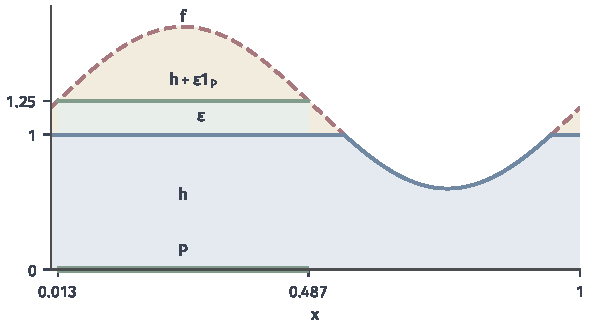
\includegraphics[width=100mm]{figures/04-spaces-measures-and-geometry/02-measure/matplotlib/dens-rn-candidate/figure.pdf}
  \caption{有限情形证明第三步的示意。参考测度为$[0,1]$上的长度，目标测度的密度$f(x)=1.2+0.6\sin(2\pi x)$（红色虚线）。候选$h=\min(f,1)$（蓝色实线）之下的质量已被表示，$h$与$f$之间的黄色区域是剩余质量$r$。取$\varepsilon=0.25$，正集$P=\{f-h\geq\varepsilon\}$约为$[0.013,0.487]$；在$P$上加高$\varepsilon$的绿色条带仍在$f$之下，所以$h+\varepsilon\mathbf 1_P$仍是候选而总积分更大。}
  \label{fig:dens-rn-candidate}
\end{BookInlineFigure}

\begin{proof}[定理~\ref{thm:dens-radon-nikodym}的证明]
先作有限分块。由$\sigma$有限性，存在两两不交的可测集$A_i$覆盖$X$且$\mu(A_i)<\infty$，以及两两不交的可测集$B_j$覆盖$X$且$\nu(B_j)<\infty$。可数族$\{A_i\cap B_j\}$两两不交、覆盖$X$，每块上$\mu,\nu$都有限，把它们排成一列$X_1,X_2,\ldots$。

再证存在性。对每个$k$，令
\[
\mu_k(A)=\mu(A\cap X_k),\qquad\nu_k(A)=\nu(A\cap X_k).
\]
这是两个有限测度，且$\nu_k\ll\mu_k$。由引理~\ref{lem:dens-rn-finite}，存在有限值可测函数$h_k$，使
\[
\nu(A\cap X_k)=\int_Ah_k\,\mathrm d\mu_k=\int_Ah_k\mathbf 1_{X_k}\,\mathrm d\mu ,
\]
后一个等号先对指示函数核对，再经简单函数与单调收敛推广。

令$h=\sum_kh_k\mathbf 1_{X_k}$，各$X_k$不交，每点至多一项非零，$h$有限且可测。由$\nu$的可数可加性与非负级数的逐项积分，
\[
\nu(A)=\sum_k\nu(A\cap X_k)=\sum_k\int_Ah_k\mathbf 1_{X_k}\,\mathrm d\mu=\int_Ah\,\mathrm d\mu .
\]

最后证唯一性。设$g:X\to[0,+\infty]$也满足等式。固定$k$，令$D=X_k\cap\{h>g\}$，则
\[
\int_Dh\,\mathrm d\mu=\nu(D)=\int_Dg\,\mathrm d\mu ,
\]
两边不超过$\nu(X_k)<\infty$，于是$\int_D(h-g)\,\mathrm d\mu=0$。被积函数在$D$上严格为正，所以$\mu(D)=0$。同理$\mu(X_k\cap\{g>h\})=0$。对$k$取可数并，$\{g\neq h\}$是$\mu$零测集。
\end{proof}

唯一性证明中只有一处用到有限性：$\nu(X_k)<\infty$才能把两个相等的积分相减。这里实际只需要$\nu$是$\sigma$有限的。缺少这一条件时唯一性可以失败：单点空间$X=\{0\}$上取$\mu(\{0\})=+\infty$，$\nu=\mu$，常数$1$与常数$2$都满足
\[
\int_{\{0\}}h\,\mathrm d\mu=+\infty=\nu(\{0\}),
\]
却在一个$\mu$测度为$+\infty$的集合上不同。所以密度只在$\mu$几乎处处的意义下唯一，而且这一唯一性依赖目标测度的$\sigma$有限性。

\paragraph{有限性条件不能随意去掉}
存在性同样依赖参考测度的$\sigma$有限性。在$[0,1]$的Borel集上取计数测度$c$与Lebesgue测度$\lambda$。$c(A)=0$只在$A=\varnothing$时成立，所以$\lambda\ll c$。若存在可测$h\geq0$使$\lambda(A)=\int_Ah\,\mathrm dc$，取$A=\{x\}$，就得到
\[
0=\lambda(\{x\})=h(x)c(\{x\})=h(x).
\]
于是$h$处处为零，却要给出$\lambda([0,1])=1$，矛盾。失效的原因在于$c$的有限测度集只能是有限集，可数个有限集之并盖不住$[0,1]$，$c$不是$\sigma$有限的。

这个反例说明定理不能无条件推广，但不说明$\sigma$有限是密度存在的必要条件。仍以$c$为参考，$\delta_0$有密度$\mathbf 1_{\{0\}}$，因为
\[
\int_A\mathbf 1_{\{0\}}\,\mathrm dc=c(A\cap\{0\})=\delta_0(A).
\]
$\sigma$有限是本章采用的一组充分条件。

\paragraph{有限有符号测度的密度}
第~\ref{chap:measure}章的有限有符号测度允许集合质量为负，它由Jordan分解写成两个有限测度之差$\eta=\eta^+-\eta^-$，总变差为$\lvert\eta\rvert=\eta^++\eta^-$。不能把上面的定理直接套到任意两个测度之差上：两个无限测度之差可能在某些集合上是$\infty-\infty$，根本没有定义。对有限有符号测度，可以对两个变差分别求密度。

\begin{theorem}[有限有符号测度的密度]
\label{thm:dens-signed}
设$\mu$是$(X,\mathcal A)$上的$\sigma$有限非负测度，$\eta$是有限有符号测度。则$\lvert\eta\rvert\ll\mu$当且仅当存在$\mu$可积的实值函数$h$，使
\begin{equation}
\eta(A)=\int_Ah\,\mathrm d\mu ,\qquad A\in\mathcal A .
\label{eq:dens-signed}
\end{equation}
此时$h$在$\mu$几乎处处意义下唯一，并且对每个$A\in\mathcal A$，
\begin{equation}
\eta^\pm(A)=\int_Ah^\pm\,\mathrm d\mu,\qquad\lvert\eta\rvert(A)=\int_A\lvert h\rvert\,\mathrm d\mu ,
\label{eq:dens-signed-parts}
\end{equation}
其中$h^+=\max(h,0)$，$h^-=\max(-h,0)$。
\end{theorem}

\begin{proof}
设$\lvert\eta\rvert\ll\mu$。由$\eta^\pm\leq\lvert\eta\rvert$得$\eta^\pm\ll\mu$。$\eta^\pm$是有限测度，由定理~\ref{thm:dens-radon-nikodym}得到有限值密度$h_1,h_2$，并且
\[
\int_Xh_1\,\mathrm d\mu=\eta^+(X)<\infty,\qquad\int_Xh_2\,\mathrm d\mu=\eta^-(X)<\infty ,
\]
二者都可积。令$h=h_1-h_2$，由可积函数积分的线性性，$h$满足式~\eqref{eq:dens-signed}。

反过来，设式~\eqref{eq:dens-signed}成立且$h$可积。令$P=\{h\geq0\}$。$P$的每个可测子集上$\eta\geq0$，补集的每个可测子集上$\eta\leq0$，所以$P$与$X\setminus P$构成$\eta$的一组Hahn分解。由Jordan分解，
\[
\eta^+(A)=\eta(A\cap P)=\int_Ah^+\,\mathrm d\mu ,
\]
\[
\eta^-(A)=-\eta(A\setminus P)=\int_Ah^-\,\mathrm d\mu .
\]
两式相加就得到$\lvert\eta\rvert$的表示，这就是式~\eqref{eq:dens-signed-parts}。由定理~\ref{thm:dens-weighted-measure}，$\lvert\eta\rvert\ll\mu$。

这一段对前一段构造的$h$同样适用，所以式~\eqref{eq:dens-signed-parts}在两个方向上都成立。

唯一性方面，若可积的$h,h'$都满足式~\eqref{eq:dens-signed}，令$D=\{h>h'\}$，则两个有限积分相等，得到
\[
\int_D(h-h')\,\mathrm d\mu=0 .
\]
被积函数在$D$上严格为正，所以$\mu(D)=0$。交换$h,h'$得$\mu(\{h'>h\})=0$，于是$h=h'$在$\mu$几乎处处成立。
\end{proof}

定理把集合层面的正负分解翻译成函数层面的正负部：Hahn分解的正区域可以取为$\{h\geq0\}$，Jordan分解的两项就是$h^+$与$h^-$分别生成的测度。可积性在这里是自然的，因为由式~\eqref{eq:dens-signed-parts}，$\lvert h\rvert$的积分就是有限的总变差$\lvert\eta\rvert(X)$。

例如$[0,1]$上$h(x)=1-2x$生成的$\eta$，正集是$P=[0,\tfrac12]$，两个变差的总质量都可以算出：
\[
\eta^+([0,1])=\int_0^{1/2}(1-2x)\,\mathrm dx=\tfrac14,\qquad\eta^-([0,1])=\int_{1/2}^1(2x-1)\,\mathrm dx=\tfrac14 .
\]
所以$\eta([0,1])=0$，正负质量完全抵消，而$\lvert\eta\rvert([0,1])=\tfrac12$记录了被抵消掉的变化总量。

\section{测度的分解}
\label{sec:dens-decomposition}

绝对连续与相互奇异是两个极端：前者不在参考测度的零测集上放任何质量，后者把全部质量放在某个参考零测集上。一般的测度介于两者之间，例如长度加上一个点质量。本节先证明，相对于给定的参考测度，$\sigma$有限测度都能唯一地拆成这两种极端之和，并用Radon–Nikodym定理表示其中绝对连续的一份。然后在实轴上以Lebesgue测度为参考，把奇异的一份再分成点质量与没有点质量的奇异质量，并说明累积函数的普通导数只能读出其中哪一部分。

\subsection{Lebesgue分解}
\label{sec:dens-lebesgue-decomposition}

给定参考测度$\mu$与目标测度$\nu$，我们希望把$\nu$的质量分成两份：一份完全落在某个$\mu$零测集上，是$\mu$“看不见”的质量；另一份在$\mu$零测集上没有任何质量。分解有三个问题需要分别回答：两份质量怎样构造，分法是否唯一，以及看得见的那份能否写成密度。

\begin{theorem}[Lebesgue分解]
\label{thm:dens-lebesgue-decomposition}
设$\mu,\nu$是可测空间$(X,\mathcal A)$上的$\sigma$有限非负测度。则存在唯一的一对非负测度$\nu_{\mathrm{ac}},\nu_{\mathrm s}$，使
\[
\nu=\nu_{\mathrm{ac}}+\nu_{\mathrm s},\qquad\nu_{\mathrm{ac}}\ll\mu,\qquad\nu_{\mathrm s}\perp\mu .
\]
更具体地，存在$N\in\mathcal A$使$\mu(N)=0$，$\nu_{\mathrm s}(A)=\nu(A\cap N)$，$\nu_{\mathrm{ac}}(A)=\nu(A\setminus N)$。并且存在可测函数$h:X\to[0,+\infty)$，使
\begin{equation}
\nu(A)=\int_Ah\,\mathrm d\mu+\nu_{\mathrm s}(A),\qquad A\in\mathcal A ,
\label{eq:dens-lebesgue-form}
\end{equation}
$h$在$\mu$几乎处处意义下唯一。特别地，$\nu$相对于$\mu$有密度，当且仅当$\nu_{\mathrm s}=0$。
\end{theorem}

这一分解称为$\nu$相对于$\mu$的\term{Lebesgue分解}（Lebesgue decomposition），$\nu_{\mathrm{ac}}$与$\nu_{\mathrm s}$分别称为绝对连续部分与奇异部分。分解依赖参考测度。在实轴上取$\nu=\lambda|_{[0,1]}+\delta_2$。以$\lambda$为参考，$N=\{2\}$是$\lambda$零测集并承载点质量，于是$\nu_{\mathrm s}=\delta_2$，$\nu_{\mathrm{ac}}=\lambda|_{[0,1]}$。以$\delta_2$为参考，$\mathbb R\setminus\{2\}$是$\delta_2$零测集，角色互换：$\nu_{\mathrm s}=\lambda|_{[0,1]}$，$\nu_{\mathrm{ac}}=\delta_2$。

\paragraph{构造：承载最多质量的零测集}
定理中的$N$应当在保持$\mu(N)=0$的同时尽可能多地装下$\nu$的质量。若某个$\mu$零测集在$N$之外还有正的$\nu$质量，就把它并进$N$。先在$\nu$有限时用上确界实现这个想法。

\begin{proof}[存在性，$\nu$有限的情形]
令$M=\sup\{\nu(A):A\in\mathcal A,\ \mu(A)=0\}\leq\nu(X)<\infty$。对每个$k$取$\mu$零测集$N_k$使$\nu(N_k)>M-1/k$，令$N=\bigcup_kN_k$。由可数次可加性$\mu(N)=0$，所以$\nu(N)\leq M$；又$\nu(N)\geq\nu(N_k)>M-1/k$，故$\nu(N)=M$。

令$\nu_{\mathrm s}(A)=\nu(A\cap N)$，$\nu_{\mathrm{ac}}(A)=\nu(A\setminus N)$，二者都是测度，和为$\nu$。由$\mu(N)=0$与$\nu_{\mathrm s}(X\setminus N)=0$得$\nu_{\mathrm s}\perp\mu$。设$\mu(A)=0$，则$N\cup(A\setminus N)$仍是$\mu$零测集，其$\nu$质量不超过$M$；两部分不交，所以$M+\nu(A\setminus N)\leq M$。$M$有限，消去得$\nu_{\mathrm{ac}}(A)=0$，即$\nu_{\mathrm{ac}}\ll\mu$。
\end{proof}

最后的消去正是需要有限性的地方：若$M=+\infty$，不等式$M+t\leq M$不能推出$t=0$。对$\sigma$有限的$\nu$，取两两不交的$X_j$覆盖$X$且$\nu(X_j)<\infty$，在每片上对有限测度$A\mapsto\nu(A\cap X_j)$作上面的构造，得到$\mu$零测集$N_j\subset X_j$；令$N=\bigcup_jN_j$，则$\mu(N)=0$。若$\mu(A)=0$，则$\nu(A\setminus N)=\sum_j\nu((A\setminus N_j)\cap X_j)=0$，每一项是相应片上已证的绝对连续性。构造只用了可数次可加性、上确界与限制测度，没有用积分。

\paragraph{唯一性}
设$\nu=\alpha+\beta=\alpha'+\beta'$，其中$\alpha,\alpha'\ll\mu$，$\beta,\beta'\perp\mu$。取$\mu$零测集$S,S'$使$\beta(X\setminus S)=0$，$\beta'(X\setminus S')=0$，令$T=S\cup S'$，则$\mu(T)=0$，$\beta,\beta'$在$X\setminus T$上都没有质量。对任意$A$，$\mu(A\cap T)=0$推出$\alpha(A\cap T)=\alpha'(A\cap T)=0$，所以$\beta(A\cap T)=\nu(A\cap T)=\beta'(A\cap T)$；又$\beta(A\setminus T)=\beta'(A\setminus T)=0$，所以$\alpha(A\setminus T)=\nu(A\setminus T)=\alpha'(A\setminus T)$。两部分相加，得$\alpha=\alpha'$，$\beta=\beta'$。

唯一性的论证只在$T$与$X\setminus T$上分别读取$\nu$，没有做减法，因此不需要任何有限性。$\sigma$有限条件只在存在性中用到，并且不能随意去掉：在$[0,1]$的Borel集上取$\mu=\lambda$，$\nu$为计数测度。若有满足要求的分解，取$N$使$\lambda(N)=0$、$\nu_{\mathrm s}([0,1]\setminus N)=0$；由于$\lambda(N)=0$，可取$x\notin N$，则$\nu_{\mathrm s}(\{x\})=0$，而$\lambda(\{x\})=0$又给出$\nu_{\mathrm{ac}}(\{x\})=0$，于是$\nu(\{x\})=0$，与计数测度矛盾。

\paragraph{密度表示}
最后一步才用到Radon–Nikodym定理。$\nu_{\mathrm{ac}}\leq\nu$，所以盖住$X$的$\nu$有限块也使$\nu_{\mathrm{ac}}$有限，$\nu_{\mathrm{ac}}$是$\sigma$有限的；对$\nu_{\mathrm{ac}}\ll\mu$应用定理~\ref{thm:dens-radon-nikodym}，得到$h=\mathrm d\nu_{\mathrm{ac}}/\mathrm d\mu$，这就是式~\eqref{eq:dens-lebesgue-form}。若另有$(h',\nu_{\mathrm s}')$满足同样的表示，则$A\mapsto\int_Ah'\,\mathrm d\mu$绝对连续（定理~\ref{thm:dens-weighted-measure}），由分解的唯一性它等于$\nu_{\mathrm{ac}}$，再由Radon–Nikodym定理的唯一性得$h'=h$几乎处处。若$\nu$有密度，则$\nu\ll\mu$，$\nu=\nu+0$就是它的分解，所以$\nu_{\mathrm s}=0$；反之$\nu_{\mathrm s}=0$时$h$就是$\nu$的密度。

三部分的依据各不相同：构造依靠可数次可加性与上确界，唯一性只读取两个集合上的值，密度表示则依靠Radon–Nikodym定理。奇异部分无论如何写不成相对于$\mu$的密度，因为它集中在一个$\mu$零测集上，而任何密度在零测集上的积分都是$0$。若目标是有限有符号测度，可以对第~\ref{chap:measure}章Jordan分解的两个变差分别作Lebesgue分解；正负分解本身回用那里的结论，这里不再重复。

\subsection{实轴测度的分解}
\label{sec:dens-real-line-decomposition}

在实轴上以$\lambda$为参考时，单点都是$\lambda$零测集，所以点质量一定属于奇异部分。问题是奇异部分是否只有点质量。下面先以实轴上的有限Borel测度为对象，把点质量完整地提出来，再说明余下的奇异部分可以不为零。

\paragraph{原子至多可数}
设$\rho$是$\mathcal B(\mathbb R)$上的有限测度。若$\rho(\{x\})>0$，称$x$是$\rho$的一个\term{原子}（atom）。

\begin{lemma}[原子至多可数]
\label{lem:dens-atoms-countable}
有限Borel测度$\rho$的原子集$D=\{x\in\mathbb R:\rho(\{x\})>0\}$至多可数。
\end{lemma}

\begin{proof}
令$D_k=\{x:\rho(\{x\})>1/k\}$，则$D=\bigcup_kD_k$。若$x_1,\ldots,x_m$是$D_k$中互不相同的点，有限可加性给出$m/k<\sum_{i=1}^m\rho(\{x_i\})\leq\rho(\mathbb R)$，所以$D_k$至多有$k\rho(\mathbb R)$个点。可数个有限集之并至多可数。
\end{proof}

于是可以定义$\rho_{\mathrm d}(B)=\rho(B\cap D)=\sum_{x\in B\cap D}\rho(\{x\})$，它是全部点质量之和，称为$\rho$的离散部分；余下的$\rho_{\mathrm c}(B)=\rho(B\setminus D)$没有原子。

\begin{theorem}[实轴上有限测度的分解]
\label{thm:dens-three-part}
设$\rho$是$\mathcal B(\mathbb R)$上的有限测度。则$\rho$可以唯一地写成
\[
\rho=\rho_{\mathrm d}+\rho_{\mathrm{ac}}+\rho_{\mathrm{sc}},
\]
其中$\rho_{\mathrm d}$集中在一个至多可数集上，$\rho_{\mathrm{ac}}\ll\lambda$，$\rho_{\mathrm{sc}}\perp\lambda$且没有原子。没有原子且与$\lambda$相互奇异的测度称为\term{奇异连续测度}（singular continuous measure）。
\end{theorem}

\begin{proof}
存在性：对有限测度$\rho_{\mathrm c}$关于$\lambda$作Lebesgue分解，得$\rho_{\mathrm c}=\rho_{\mathrm{ac}}+\rho_{\mathrm{sc}}$，而$\rho_{\mathrm{sc}}(\{x\})\leq\rho_{\mathrm c}(\{x\})=0$。

唯一性：设$\rho=d+a+s$也满足条件，$d$集中在至多可数集$D'$上。$a\ll\lambda$给出$a(\{x\})=0$，$s$没有原子，所以$\rho(\{x\})=d(\{x\})$对每个$x$成立。于是$D\subset D'$，并且$d(B)=\sum_{x\in B\cap D'}d(\{x\})=\sum_{x\in B\cap D}\rho(\{x\})=\rho_{\mathrm d}(B)$，因为$D'\setminus D$中的点质量为零。由此$a+s=\rho-d=\rho_{\mathrm c}$（各项有限，减法有意义），再由Lebesgue分解的唯一性得$a=\rho_{\mathrm{ac}}$，$s=\rho_{\mathrm{sc}}$。
\end{proof}

离散部分集中在可数集上，与$\lambda$相互奇异，所以$\rho$相对于$\lambda$的奇异部分就是$\rho_{\mathrm d}+\rho_{\mathrm{sc}}$。三项是同一个测度的三个成分，一个测度可以同时含有三者，也可以缺少其中任意几项。

定理只对有限测度陈述。推广到$\sigma$有限的Borel测度时需要核对两点。其一，原子集仍至多可数：取测度有限且覆盖$\mathbb R$的可测集$X_1,X_2,\ldots$，每个原子落在某个$X_k$中，对有限测度$B\mapsto\rho(B\cap X_k)$用引理~\ref{lem:dens-atoms-countable}，可知$X_k$中的原子至多可数。其二，唯一性证明中的减法$\rho-d$可能出现$\infty-\infty$，应改为把各成分限制到每个$X_k$上分别比较。局部有限测度，即在每个有界区间上取有限值的测度，用$X_k=(k-1,k]$与$(-k,-k+1]$即可覆盖，是最常见的情形，例如Lebesgue测度本身。

\paragraph{累积函数读出原子}
离散部分可以从累积函数读出。记$G(x)=\rho((-\infty,x])$。集合$(-\infty,x-1/m]$递增到$(-\infty,x)$，由测度的从下连续性，左极限$G(x-)=\rho((-\infty,x))$，所以
\[
G(x)-G(x-)=\rho(\{x\}).
\]
$G$在$x$处跳跃当且仅当$x$是原子，$G$连续当且仅当$\rho_{\mathrm d}=0$。累积函数连续能排除离散部分，却不能排除奇异连续部分。下面的Cantor测度说明后者确实存在。

\paragraph{Cantor测度}
第~\ref{chap:integration}章构造了Cantor集$C\subset[0,1]$与Cantor函数$F_C$：$C$由逐步删去中间三分之一开区间得到，Lebesgue测度为零；$F_C$连续、单调不减，$F_C(0)=0$，$F_C(1)=1$，并在每个删去的开区间上为常数。把$F_C$延拓为$x<0$时取$0$、$x>1$时取$1$，延拓后的函数连续、单调不减，按第~\ref{chap:measure}章的Stieltjes构造得到Borel测度$\mu_C$，满足$\mu_C((a,b])=F_C(b)-F_C(a)$，称为\term{Cantor测度}（Cantor measure）。

它的三条性质可以直接核对。总质量为$F_C(1)-F_C(0)=1$。没有原子：$F_C$连续，所以$\mu_C(\{x\})=F_C(x)-F_C(x-)=0$。集中在$C$上：在每个删去的开区间$(a,b)$上$F_C$为常数，由从下连续性$\mu_C((a,b))=\lim_m(F_C(b-1/m)-F_C(a))=0$，两条半直线同理；$\mathbb R\setminus C$是这些开区间与两条半直线的可数并，故$\mu_C(\mathbb R\setminus C)=0$。又$\lambda(C)=0$，取$N=C$即得$\mu_C\perp\lambda$。所以$\mu_C$是一个非零的奇异连续测度。

\begin{example}[三种成分的混合]
\label{ex:dens-three-part-mixture}
令$\rho=\tfrac12\lambda|_{[0,1]}+\tfrac14\delta_{1/2}+\tfrac14\mu_C$，总质量$\tfrac12+\tfrac14+\tfrac14=1$。$\lambda$与$\mu_C$都没有原子，唯一的原子是$1/2$，所以$\rho_{\mathrm d}=\tfrac14\delta_{1/2}$。余下的$\tfrac12\lambda|_{[0,1]}+\tfrac14\mu_C$相对于$\lambda$作Lebesgue分解，取$N=C$：前一项在$C$上为零，后一项集中在$C$上，于是$\rho_{\mathrm{ac}}=\tfrac12\lambda|_{[0,1]}$，$\rho_{\mathrm{sc}}=\tfrac14\mu_C$。按式~\eqref{eq:dens-lebesgue-form}，$\rho$相对于$\lambda$的密度部分是$h=\tfrac12\mathbf 1_{[0,1]}$，图~\ref{fig:dens-lebesgue-form}画出了这三部分。
\end{example}

\begin{figure}[!htbp]
  \centering
  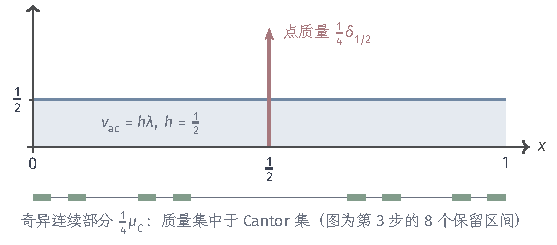
\includegraphics[width=94.365mm]{figures/02-abstract-mathematics/01-metric-and-measure/tikz/c4-lebesgue-density/figure.pdf}
  \caption{相对于长度测度的密度只表示绝对连续部分。$\rho=\tfrac12\lambda|_{[0,1]}+\tfrac14\delta_{1/2}+\tfrac14\mu_C$：蓝色区域是密度$h=1/2$表示的质量$1/2$；红色箭头是位于$1/2$的点质量$1/4$；下方绿色线段是Cantor集构造第$3$步保留的$8$个区间，Cantor测度的质量$1/4$集中在它们的极限——零长度的Cantor集上。后两部分都集中在长度零测集上，任何密度都无法表示。}
  \label{fig:dens-lebesgue-form}
\end{figure}

\paragraph{普通导数能恢复什么}
这个例子的累积函数在$[0,1]$上是$G(x)=\tfrac12x+\tfrac14\mathbf 1_{[1/2,\infty)}(x)+\tfrac14F_C(x)$。求它的普通导数：一次项的导数是$\tfrac12$；阶跃项在$x\neq1/2$处导数为零；Cantor函数在每个删去的开区间上为常数，而这些开区间的总长度为$1$，所以它几乎处处导数为零。于是$G'=\tfrac12$几乎处处，恰好是绝对连续部分的密度。

导数遗漏了另外两份质量：$\int_0^1G'\,\mathrm dx=\tfrac12$，而$G(1)-G(0)=1$，差额中$\tfrac14$是原点$1/2$处的跳跃，另$\tfrac14$是Cantor函数在零长度集合上的连续增长。这正是第~\ref{chap:integration}章所说的：连续性与几乎处处可导都不能保证函数由导数的积分恢复。一般地，实轴上有限Borel测度的累积函数几乎处处可导，导数几乎处处等于绝对连续部分的密度；这一结论属于Lebesgue微分定理，这里不给出证明。本章只在累积函数绝对连续时使用导数计算密度，见第~\ref{sec:dens-cumulative-density}小节。

\section{密度的运算}
\label{sec:dens-rules}

有了密度以后，最常用的操作都围绕“换参考测度”：把对目标测度的积分改写成对参考测度的加权积分；把几个目标测度相对同一参考的密度组合起来；经过一个中间测度连续换两次参考；或者把参考与目标的角色对调。本节在同一可测空间$(X,\mathcal A)$上依次建立这些规则，每条规则都注明所需的测度关系，以及等式在哪个测度的几乎处处意义下成立。

\subsection{换测度的积分公式}
\label{sec:dens-change-of-measure}

密度的定义~\eqref{eq:dens-definition}只说明指示函数$\mathbf 1_A$对$\nu$的积分等于$\mathbf 1_Ah$对$\mu$的积分。积分本来就是从指示函数出发，经简单函数和单调逼近推广到一般函数的，所以这个等式可以沿同一条路线推广。

\begin{theorem}[换测度公式]
\label{thm:dens-change-of-measure}
设$\mu,\nu$是$(X,\mathcal A)$上的非负测度，$h$是$\nu$相对于$\mu$的密度，约定$0\cdot(+\infty)=0$。
\begin{enumerate}
\item 对每个可测函数$f:X\to[0,+\infty]$，
\begin{equation}
\int_Xf\,\mathrm d\nu=\int_Xfh\,\mathrm d\mu .
\label{eq:dens-change-of-measure}
\end{equation}
\item 对实值或复值可测函数$f$，$f$对$\nu$可积当且仅当$fh$对$\mu$可积，此时式~\eqref{eq:dens-change-of-measure}成立。
\end{enumerate}
\end{theorem}

\begin{proof}
(1) 对$f=\mathbf 1_A$，两边分别是$\nu(A)$与$\int_Ah\,\mathrm d\mu$，由密度的定义相等。对非负简单函数，两边对$f$都是线性的，等式成立。对一般非负可测$f$，取非负简单函数列$s_n\uparrow f$。因$h\geq0$，$s_nh$也递增并逐点收敛到$fh$。两边分别用单调收敛定理，
\[
\int_Xf\,\mathrm d\nu=\lim_{n\to\infty}\int_Xs_n\,\mathrm d\nu=\lim_{n\to\infty}\int_Xs_nh\,\mathrm d\mu=\int_Xfh\,\mathrm d\mu ,
\]
两边允许同时为$+\infty$。

(2) 对$\lvert f\rvert$用(1)，得$\int\lvert f\rvert\,\mathrm d\nu=\int\lvert fh\rvert\,\mathrm d\mu$，两种可积性等价。实值时$(fh)^\pm=f^\pm h$，对$f^+,f^-$分别用(1)，各得两个有限数，相减即得等式。复值时对实部和虚部分别处理。
\end{proof}

\term{换测度公式}（change-of-measure formula）把“对目标测度累计”改写成“对参考测度加权累计”。被积的变量与函数$f$都不变，点不移动，改变的只是每一处的累计权重。例如$[0,1]$上$\nu$相对于长度的密度为$h(x)=2x$，取$f(x)=x$，则$\int f\,\mathrm d\nu=\int_0^1x\cdot2x\,\mathrm dx=\tfrac23$；若$\nu$是概率测度，这就是用概率密度计算期望的公式。

两部分的条件不同。非负函数不需要任何可积性，等式两边可以同为$+\infty$；实值或复值函数则必须先由$\lvert f\rvert$确认两边绝对可积，否则正部与负部的积分可能都是$+\infty$，不能相减。证明中没有用到$\mu,\nu$的有限性：只要密度存在，公式就成立。

\subsection{密度的线性组合}
\label{sec:dens-linear-combination}

相对同一个参考测度，几个目标测度组合起来时，密度怎样组合？非负组合可以直接相加；带符号的组合还要先保证测度之差有定义。

\paragraph{共同参考下的非负组合}
设$\nu_1,\ldots,\nu_m$相对于同一个参考测度$\mu$分别有密度$h_1,\ldots,h_m$，$a_1,\ldots,a_m\geq0$。由非负积分的线性性，对每个可测集$A$，
\[
\sum_{i=1}^ma_i\nu_i(A)=\sum_{i=1}^ma_i\int_Ah_i\,\mathrm d\mu=\int_A\sum_{i=1}^ma_ih_i\,\mathrm d\mu ,
\]
所以$\sum_ia_i\nu_i$的密度是$\sum_ia_ih_i$。关键是参考测度相同：密度是相对于参考的换算比例，只有同一种参考下的比例才能直接相加。非负系数的可数和同样成立，此时交换求和与积分的依据是单调收敛定理。

共同参考还能把一个相对于长度没有密度的测度写成单个函数的积分。

\begin{example}[点质量与长度的统一表示]
\label{ex:dens-mixed-reference}
在$[0,1]$上取参考测度$\mu=\lambda|_{[0,1]}+\delta_0$。对可测集$A\subset[0,1]$，
\begin{equation*}
\begin{aligned}
\int_A\mathbf 1_{(0,1]}\,\mathrm d\mu&=\lambda(A\cap(0,1])+\delta_0(A\cap(0,1])=\lambda(A),\\
\int_A\mathbf 1_{\{0\}}\,\mathrm d\mu&=\lambda(A\cap\{0\})+\delta_0(A\cap\{0\})=\delta_0(A),
\end{aligned}
\end{equation*}
其中用了$\lambda(\{0\})=0$与$0\notin(0,1]$。所以$\mathrm d\lambda|_{[0,1]}/\mathrm d\mu=\mathbf 1_{(0,1]}$，$\mathrm d\delta_0/\mathrm d\mu=\mathbf 1_{\{0\}}$。由线性组合规则，$a,b\geq0$时$\nu=a\lambda|_{[0,1]}+b\delta_0$的密度是$a\mathbf 1_{(0,1]}+b\mathbf 1_{\{0\}}$。当$b>0$时$\nu$在长度零测集$\{0\}$上有正质量，整体没有Lebesgue密度；换用共同参考$\mu$后，点质量与长度质量就由一个函数统一表示。
\end{example}

例中原点处的密度值$b$不能随意改动：原点在$\mu$下质量为$1$，不是$\mu$零测集。这与长度参考不同，那里单点上的取值可以任意改变。哪些点上的密度值有意义，取决于参考测度在那里有没有质量。

\paragraph{带符号的组合}
差需要谨慎处理。若$\nu_1,\nu_2$是有限测度，则$h_1,h_2$可积，$\eta=a\nu_1-b\nu_2$（$a,b$为实数）是有限有符号测度，由可积函数积分的线性性，它的密度是可积函数$ah_1-bh_2$，与定理~\ref{thm:dens-signed}一致。对无限测度不能这样做：在$\mathbb R$上取$\nu_1=\nu_2=\lambda$，形式上$h_1-h_2=0$，可$\nu_1(\mathbb R)-\nu_2(\mathbb R)=\infty-\infty$没有定义，“$\nu_1-\nu_2$”不是在所有集合上都有值的对象。更一般地，只要对相减的两项在所考虑的每个集合上都有$\int_Ah_2\,\mathrm d\mu<\infty$，差才有意义。


\subsection{链式规则}
\label{sec:dens-chain-rule}

换算比例可以连乘：先从一种参考换到中间测度，再从中间测度换到目标。为避免与Lebesgue测度的记号冲突，本小节用$\rho$表示最底层的参考测度。

\begin{theorem}[密度的链式规则]
\label{thm:dens-chain-rule}
设$\rho,\mu,\nu$是$(X,\mathcal A)$上的$\sigma$有限非负测度，且$\nu\ll\mu\ll\rho$。则$\nu\ll\rho$，并且
\[
\frac{\mathrm d\nu}{\mathrm d\rho}=\frac{\mathrm d\nu}{\mathrm d\mu}\cdot\frac{\mathrm d\mu}{\mathrm d\rho}\qquad\rho\text{几乎处处}.
\]
\end{theorem}

\begin{proof}
由Radon–Nikodym定理取$g=\mathrm d\nu/\mathrm d\mu$与$k=\mathrm d\mu/\mathrm d\rho$。对任意可测集$A$，先用$g$的定义，再对非负函数$\mathbf 1_Ag$与密度$k$使用换测度公式，
\[
\nu(A)=\int_X\mathbf 1_Ag\,\mathrm d\mu=\int_X\mathbf 1_Agk\,\mathrm d\rho .
\]
所以$gk$是$\nu$相对于$\rho$的一个密度，由定理~\ref{thm:dens-weighted-measure}得$\nu\ll\rho$。$\nu,\rho$都$\sigma$有限，由Radon–Nikodym定理的唯一性，任何版本的$\mathrm d\nu/\mathrm d\rho$都与$gk$在$\rho$几乎处处意义下相等。
\end{proof}

这条\term{密度的链式规则}（chain rule for densities）与一元微积分的链式法则形式相似，依据却是换测度公式，而不是对坐标求导。逐次换参考与直接换参考给出同一个积分表示：对非负$f$，$\int f\,\mathrm d\nu=\int fg\,\mathrm d\mu=\int fgk\,\mathrm d\rho$。数值例子：$[0,1]$上$\rho=\lambda|_{[0,1]}$，$\mathrm d\mu/\mathrm d\rho=2x$，$\mathrm d\nu/\mathrm d\mu=\tfrac32x$，链式规则给出$\mathrm d\nu/\mathrm d\rho=3x^2$。直接核对：$\mu([0,1])=\int_0^12x\,\mathrm dx=1$，$\nu([0,1])=\int_0^1\tfrac32x\cdot2x\,\mathrm dx=\int_0^13x^2\,\mathrm dx=1$。图~\ref{fig:dens-chain-rule}画出了两段换算。

\begin{figure}[!htbp]
  \centering
  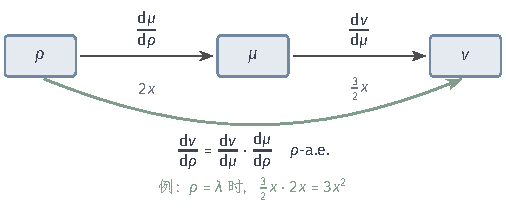
\includegraphics[width=85.651mm]{figures/02-abstract-mathematics/01-metric-and-measure/tikz/c4-chain-rule/figure.pdf}
  \caption{密度的链式规则。箭头表示“箭头终点的测度相对于起点测度的密度”：先从$\rho$换到$\mu$，再从$\mu$换到$\nu$，两段密度相乘就是从$\rho$直接换到$\nu$的密度（绿色弧线），等式在$\rho$几乎处处意义下成立。箭头下方是$[0,1]$上$\rho=\lambda$时的例子，$2x$与$\tfrac32x$相乘得到$3x^2$。}
  \label{fig:dens-chain-rule}
\end{figure}

\paragraph{各因子的几乎处处意义}
$g=\mathrm d\nu/\mathrm d\mu$只确定到$\mu$零测集，而结论是关于$\rho$零测集的。两者并不冲突。设$g'$是$g$的另一个版本，$g\neq g'$只发生在某个$\mu$零测集$M$上，于是乘积$gk$与$g'k$只可能在$M\cap\{k>0\}$上不同。由$0=\mu(M)=\int_Mk\,\mathrm d\rho$，$k$在$M$上$\rho$几乎处处为零，所以$\rho(M\cap\{k>0\})=0$。也就是说，在$k=0$处乘积按约定取$0$，与$g$的取值无关；在$k>0$处，$\mu$的零测例外也是$\rho$的零测例外。无论选哪个版本，乘积都给出同一个$\rho$几乎处处确定的密度。

\subsection{倒数规则}
\label{sec:dens-inverse-rule}

若两个测度相互绝对连续，就可以从任一方换到另一方。反向的密度应当是原密度的倒数，但这需要先保证原密度几乎处处既不为零也不为无穷。

\begin{theorem}[密度的倒数]
\label{thm:dens-inverse}
设$\mu,\nu$是$(X,\mathcal A)$上的$\sigma$有限非负测度，$\nu\ll\mu$且$\mu\ll\nu$，$h=\mathrm d\nu/\mathrm d\mu$。则$0<h<\infty$在$\mu$几乎处处成立，并且
\[
\frac{\mathrm d\mu}{\mathrm d\nu}=\frac1h ,
\]
等式在$\mu$几乎处处意义下成立，也在$\nu$几乎处处意义下成立。
\end{theorem}

\begin{proof}
由Radon–Nikodym定理可取有限值的$h$。令$Z=\{h=0\}$，则$\nu(Z)=\int_Zh\,\mathrm d\mu=0$，由$\mu\ll\nu$得$\mu(Z)=0$，所以$0<h<\infty$在$\mu$几乎处处成立。令$u=1/h$于$X\setminus Z$，$u=0$于$Z$。对任意可测集$A$，由换测度公式，
\[
\int_Au\,\mathrm d\nu=\int_X\mathbf 1_Auh\,\mathrm d\mu=\mu(A\setminus Z)=\mu(A),
\]
所以$u$是$\mu$相对于$\nu$的密度。两个测度等价，零测集相同，因此$\mu$几乎处处与$\nu$几乎处处是同一回事。
\end{proof}

这个结论也可以从链式规则读出：对$\mu\ll\nu\ll\mu$用定理~\ref{thm:dens-chain-rule}，得$(\mathrm d\mu/\mathrm d\nu)\cdot h=\mathrm d\mu/\mathrm d\mu=1$。例如$[0,1]$上$\nu$相对于$\lambda$的密度为$2x$，它只在零测集$\{0\}$上为零，所以$\nu$与$\lambda|_{[0,1]}$等价，反向密度为$1/(2x)$，$x\in(0,1]$。反向密度无界，但仍满足$\int_0^1\frac1{2x}\cdot2x\,\mathrm dx=1=\lambda([0,1])$。

\paragraph{单向绝对连续时的信息丢失}
若只有$\nu\ll\mu$，密度$h$可以在一个正$\mu$测度的区域上为零。取$\mu=\lambda|_{[0,2]}$，$\nu=\lambda|_{[0,1]}$，则$h=\mathbf 1_{[0,1]}$。在正密度区域$\{h>0\}=[0,1]$上，反向表示仍然成立：对$A\subset\{h>0\}$，$\mu(A)=\int_A(1/h)\,\mathrm d\nu$。但在零密度区域$(1,2]$上，$\mu$有质量$1$，$\nu$却为零，无论用什么函数加权，$\int_{(1,2]}u\,\mathrm d\nu$都是$0$，不可能恢复$\mu((1,2])=1$。这时$\mu$并不相对于$\nu$绝对连续，整体的反向密度不存在。图~\ref{fig:dens-one-sided-loss}显示了这块被目标测度完全忽略的区域。

\begin{figure}[!htbp]
  \centering
  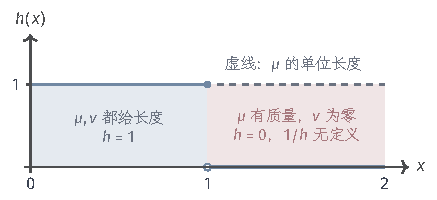
\includegraphics[width=73.914mm]{figures/02-abstract-mathematics/01-metric-and-measure/tikz/c4-one-sided-loss/figure.pdf}
  \caption{单向绝对连续时密度不能取倒数。参考测度$\mu$是$[0,2]$上的长度，目标测度$\nu$是$[0,1]$上的长度，密度$h=\mathbf 1_{[0,1]}$（蓝色实线）。在$[0,1]$上$h=1$，两种测度一致；在红色区域$(1,2]$上$h=0$，$\mu$有质量$1$而$\nu$没有质量，从$\nu$出发无法恢复这部分质量。}
  \label{fig:dens-one-sided-loss}
\end{figure}

一般地，若$\nu\ll\mu$且都$\sigma$有限，令$P=\{h>0\}$，同样的计算给出$\mu(A\cap P)=\int_A\mathbf 1_P/h\,\mathrm d\nu$，即$1/h$是$\mu|_P$相对于$\nu$的密度。原参考测度在零密度区域$X\setminus P$上的质量$\mu|_{X\setminus P}$与$\nu$相互奇异，这正是$\mu$相对于$\nu$的Lebesgue分解中的奇异部分，不能通过相除恢复。倒数公式只能在两个测度等价的范围内整体使用。

\section{密度的计算}
\label{sec:dens-computation}

前几节回答了密度何时存在、怎样使用。本节回到两类具体对象：可数集合上由点质量给出的测度，以及实轴上由累积函数的增量给出的测度。每个例子都按同一顺序处理：先固定参考测度，检查绝对连续性，再求密度，最后代入换测度公式核对它能否恢复目标测度的质量与积分。

\subsection{离散测度的密度}
\label{sec:dens-discrete}

可数集合上每个点都可以单独称量，所以离散测度的密度可以逐点计算，这是向量类比完全成立的情形。需要分别处理的只是参考质量为零的点。

\paragraph{点质量之比}
设$X=\{x_1,x_2,\ldots\}$是可数集合，取全部子集为可测集，参考测度与目标测度分别为
\[
\mu=\sum_im_i\delta_{x_i},\qquad\nu=\sum_ip_i\delta_{x_i},\qquad m_i,p_i\in[0,+\infty).
\]
单点质量有限，可数个单点覆盖$X$，所以两者都$\sigma$有限。

先检查绝对连续。$\mu(A)=0$当且仅当$A$中每点的$m_i$都为零，所以$\nu\ll\mu$当且仅当“$m_i=0$推出$p_i=0$”。在此条件下令
\begin{equation}
h(x_i)=\frac{p_i}{m_i}\quad(m_i>0),\qquad h(x_i)\ \text{取任意非负值}\quad(m_i=0).
\label{eq:dens-discrete}
\end{equation}

对离散测度的积分是加权求和，于是对任意$A\subset X$，
\[
\begin{aligned}
\int_Ah\,\mathrm d\mu&=\sum_{x_i\in A}h(x_i)m_i=\sum_{x_i\in A,\,m_i>0}p_i\\
&=\sum_{x_i\in A}p_i=\nu(A),
\end{aligned}
\]
第三个等号用到$m_i=0$时$p_i=0$。所以$h$是$\nu$相对于$\mu$的密度。

两类点的处理不同。参考质量为正的点上，密度值就是质量之比，被唯一确定。参考质量为零的点构成$\mu$零测集，密度在那里可以任意取值，这正是几乎处处版本在离散情形的样子。以计数测度为参考时所有$m_i=1$，密度就是目标的点质量本身，即概率质量函数。

\paragraph{参考零测点上的目标质量}
若某点$m_i=0$而$p_i>0$，不能用“取一个很大的有限比值”来补救：任何有限或无限的$h(x_i)$都满足$h(x_i)m_i=0\neq p_i$。这时的问题不在于比值难算，而在于$\nu\ll\mu$不成立，密度根本不存在。

正确的做法是先作Lebesgue分解。令$N=\{x_i:m_i=0\}$，则$\nu$的奇异部分与绝对连续部分分别是
\[
\nu_{\mathrm s}=\sum_{x_i\in N}p_i\delta_{x_i},\qquad\nu_{\mathrm{ac}}=\sum_{x_i\notin N}p_i\delta_{x_i} ,
\]
只有$\nu_{\mathrm{ac}}$才有密度$p_i/m_i$。

例如在$X=\{0,1,2\}$上取
\[
\mu=\delta_0+\delta_1,\qquad\nu=\tfrac12\delta_0+\tfrac14\delta_1+\tfrac14\delta_2 ,
\]
则$N=\{2\}$，点$2$上的质量$\tfrac14$是奇异部分。$\nu_{\mathrm{ac}}$的密度在$0,1$处分别为$\tfrac12,\tfrac14$。

\begin{example}[同一分布换两种参考]
\label{ex:dens-poisson}
在$\{0,1,2,\ldots\}$上取参数为$1$的Poisson分布$p_k=\mathrm e^{-1}/k!$为目标。相对于计数测度，密度就是$p_k$本身。若改用几何权重$m_k=2^{-(k+1)}$作参考，所有$m_k>0$，密度为
\[
h(k)=\frac{p_k}{m_k}=\frac{2^{k+1}\mathrm e^{-1}}{k!} .
\]
前六项约为
\[
0.736,\quad1.472,\quad1.472,\quad0.981,\quad0.491,\quad0.196 .
\]
核对集合$\{0,1\}$的质量。直接求和与加权求和分别是
\[
\begin{aligned}
\nu(\{0,1\})&=2\mathrm e^{-1}\approx0.7358,\\
h(0)m_0+h(1)m_1&\approx0.7358\cdot0.5+1.4715\cdot0.25\approx0.7358 ,
\end{aligned}
\]
两者一致。两种密度由链式规则联系：几何权重相对于计数测度的密度是$m_k$，所以$h(k)\cdot m_k=p_k$。
\end{example}

图~\ref{fig:dens-discrete}画出了两组点质量及它们的比值。比值大于$1$的地方，目标比参考更重；$k$增大后几何权重比阶乘倒数衰减得慢，比值趋于零。

\begin{BookInlineFigure}
  \centering
  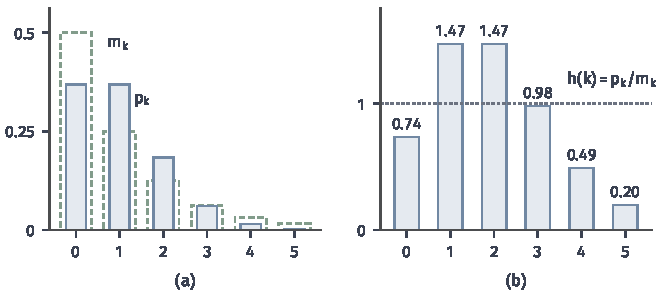
\includegraphics[width=112mm]{figures/04-spaces-measures-and-geometry/02-measure/matplotlib/dens-discrete/figure.pdf}
  \caption{可数集合上的离散密度。(a)绿色虚线框为几何参考质量$m_k=2^{-(k+1)}$，蓝色柱为Poisson目标质量$p_k=\mathrm e^{-1}/k!$，$k=0,\ldots,5$。(b)密度$h(k)=p_k/m_k$：$k=1,2$处目标质量相对参考最多，$h$约为$1.47$；$k$增大后$h$趋于零。}
  \label{fig:dens-discrete}
\end{BookInlineFigure}

密度的计算与总质量是否有限无关。仍以几何权重为参考，计数测度$\sum_k\delta_k$的密度是$h(k)=2^{k+1}$，目标的总质量为$+\infty$，但每个集合上的质量都由$h$正确恢复。代入换测度公式，例如对$f(k)=k$，
\[
\sum_kk\,p_k=\sum_kk\,\frac{p_k}{m_k}\,m_k ,
\]
两边都是Poisson分布的均值$1$。

\subsection{由累积函数求密度}
\label{sec:dens-cumulative-density}

实轴上的测度常常由累积函数给出。设$F:\mathbb R\to\mathbb R$单调不减且右连续，第~\ref{chap:measure}章的Stieltjes构造给出Borel测度$\mu_F$，满足$\mu_F((s,t])=F(t)-F(s)$。它在每个有界区间上有限，因而$\sigma$有限。我们要问$\mu_F$何时有Lebesgue密度，以及密度怎样从$F$算出。

\begin{theorem}[累积函数的密度]
\label{thm:dens-cumulative}
设$F:\mathbb R\to\mathbb R$单调不减且右连续。
\begin{enumerate}
\item 若$F$在每个有界闭区间上绝对连续，则$\mu_F\ll\lambda$，并且
\begin{equation}
\frac{\mathrm d\mu_F}{\mathrm d\lambda}=F'\qquad\lambda\text{几乎处处}.
\label{eq:dens-cumulative}
\end{equation}
\item 反之，若$\mu_F\ll\lambda$，则$F$在每个有界闭区间上绝对连续。
\end{enumerate}
\end{theorem}

\begin{proof}
(1) 由第~\ref{chap:integration}章，绝对连续函数几乎处处可导，导数局部可积，并且
\[
F(t)-F(s)=\int_s^tF'(x)\,\mathrm dx .
\]
$F$单调不减，在可导点差商非负，所以$F'\geq0$几乎处处，可以取非负版本。

令$\nu(A)=\int_AF'\,\mathrm d\lambda$。由定理~\ref{thm:dens-weighted-measure}它是测度，并且在每个区间$(s,t]$上与$\mu_F$相等。两者在每个$(-m,m]$上有限；半开区间族对交封闭并生成Borel $\sigma$代数，由第~\ref{chap:measure}章测度延拓的唯一性，$\nu=\mu_F$。于是$F'$是$\mu_F$相对于$\lambda$的密度，$\mu_F\ll\lambda$。

(2) 固定$[a,b]$。$\lambda$是$\sigma$有限的，由Radon–Nikodym定理存在非负可测$h$使$\mu_F(A)=\int_Ah\,\mathrm d\lambda$，并且
\[
\int_a^bh\,\mathrm dx=F(b)-F(a)<\infty .
\]
于是对$x\in[a,b]$，
\[
F(x)=F(a)+\mu_F((a,x])=F(a)+\int_a^xh(t)\,\mathrm dt .
\]
可积函数的变上限积分绝对连续，所以$F$在$[a,b]$上绝对连续。
\end{proof}

定理把函数的绝对连续与测度的绝对连续联系起来：对单调累积函数，“总长度小的区间组上增量之和小”恰好对应“长度零测集上没有增量质量”。密度就是导数，但只在几乎处处意义下确定：$F$在个别点上可以没有导数，在那里给密度取什么值都不影响$\mu_F$。

\begin{example}[多项式累积函数]
\label{ex:dens-square-cdf}
令$F(x)=0$（$x<0$），$F(x)=x^2$（$0\leq x\leq1$），$F(x)=1$（$x>1$）。$F$在每个有界闭区间上是Lipschitz的，因而绝对连续，于是$\mu_F$相对于$\lambda$的密度是
\[
F'(x)=2x\mathbf 1_{(0,1)}(x).
\]
在$x=1$处$F$没有导数，但单点不影响密度。代入换测度公式，
\[
\int x\,\mathrm d\mu_F=\int_0^1x\cdot2x\,\mathrm dx=\tfrac23 ,
\]
与第~\ref{sec:dens-change-of-measure}小节的例子一致。
\end{example}

\paragraph{检查原子与奇异连续部分}
定理的条件不能省略，也不能只检查$F$是否连续。计算一般累积函数的密度时，应当按第~\ref{sec:dens-decomposition}节的分解逐项检查。第一步读出跳跃：由式~\eqref{eq:dens-jump}的同一推导，$F(x)-F(x-)=\mu_F(\{x\})$，跳跃点就是原子。第二步去掉跳跃后检查余下的连续部分是否绝对连续；若是，它的导数就是$\mu_F$的绝对连续部分的密度，否则还有奇异连续部分。只把$F'$当作整个测度的密度，会同时漏掉这两类质量。

\begin{example}[有跳跃的累积函数]
\label{ex:dens-mixed-cdf}
令
\[
F(x)=\begin{cases}0,&x<0,\\\tfrac12+\tfrac x2,&0\leq x<1,\\1,&x\geq1.\end{cases}
\]
$F$在$0$处从$0$跳到$\tfrac12$，其余处连续，所以$\mu_F$有原子$0$，质量$\tfrac12$。去掉跳跃后的$F-\tfrac12\mathbf 1_{[0,\infty)}$在$[0,1]$上是$\tfrac x2$，绝对连续，导数$\tfrac12$。于是
\[
\mu_F=\tfrac12\delta_0+\tfrac12\lambda|_{[0,1]} ,
\]
只有后一项有Lebesgue密度$\tfrac12\mathbf 1_{[0,1]}$。

用换测度公式检验差别。取$g(x)=1+x$，正确的积分把原子和密度两部分都算上：
\[
\int g\,\mathrm d\mu_F=\tfrac12g(0)+\int_0^1\tfrac12(1+x)\,\mathrm dx=\tfrac12+\tfrac34=\tfrac54 .
\]
若误把$F'$当作整个测度的密度，只得到
\[
\int_0^1(1+x)\cdot\tfrac12\,\mathrm dx=\tfrac34 ,
\]
恰好漏掉原子贡献的$\tfrac12g(0)=\tfrac12$。
\end{example}

图~\ref{fig:dens-cumulative-jump}左边是累积函数，右边是它对应的测度。左图的跳跃高度变成右图的箭头，左图的斜率变成右图的密度。

\begin{BookInlineFigure}
  \centering
  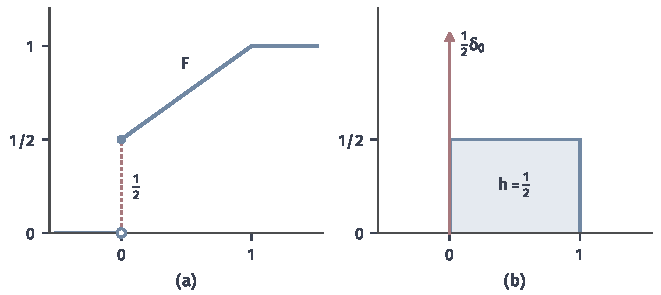
\includegraphics[width=112mm]{figures/04-spaces-measures-and-geometry/02-measure/matplotlib/dens-cumulative-jump/figure.pdf}
  \caption{有跳跃的累积函数与它的测度。(a)$F$在$0$处跳跃$\tfrac12$（红色虚线），在$(0,1)$上斜率为$\tfrac12$。(b)对应的测度$\mu_F=\tfrac12\delta_0+\tfrac12\lambda|_{[0,1]}$：红色箭头是原子，蓝色区域是密度$\tfrac12$表示的连续质量。}
  \label{fig:dens-cumulative-jump}
\end{BookInlineFigure}

连续却不绝对连续的情形由Cantor函数给出。第~\ref{sec:dens-real-line-decomposition}小节的混合例子中，去掉跳跃后的$\tfrac x2+\tfrac14F_C(x)$已经连续，却仍有$\tfrac14$的奇异连续质量，其导数几乎处处等于$\tfrac12$，只恢复绝对连续部分。所以“$F$连续”“$F$几乎处处可导”都不足以让导数成为整个测度的密度，必须要求绝对连续。

对右连续的有界变差函数，增量可以为负。这时可以先写成两个单调函数之差，再对两个Stieltjes测度分别应用本小节的步骤，最后按有限有符号测度的规则相减。

\section{本章小结}
\label{sec:dens-summary}

本章开头问：一个测度何时能写成参考测度的加权积分，权重怎样计算，有了权重之后积分怎样改写。全章可以对照有限点集上的向量来读，表~\ref{tab:dens-vector-analogy}列出了对应关系，以及类比失效之后一般情形用什么代替。

\begin{BookInlineTable}
\small
\begin{tabular}{@{}>{\RaggedRight\arraybackslash}p{22mm}>{\RaggedRight\arraybackslash}p{\dimexpr(\linewidth-22mm-4\tabcolsep)*2/5\relax}>{\RaggedRight\arraybackslash}p{\dimexpr(\linewidth-22mm-4\tabcolsep)*3/5\relax}@{}}
\toprule
概念 & 有限点集上的向量 & 一般测度\\
\midrule
测度 & 非负向量 & 集合上的可数可加函数\\
绝对连续 & 零分量位置的包含 & 对每个可测集检查零测关系\\
相互奇异 & 两向量无公共正分量 & 用一个可测集分开，闭支撑可以相交\\
密度 & 逐分量比值 & 无逐点比值，由集合上的积分等式确定\\
Lebesgue分解 & 按$m_i>0$与否分下标 & 寻找承载最多质量的零测集\\
换参考 & 对角矩阵乘向量 & 换测度公式\\
连续换参考 & 对角矩阵相乘 & 链式规则，几乎处处成立\\
对调参考与目标 & 对角矩阵求逆 & 倒数规则，要求两个测度等价\\
\bottomrule
\end{tabular}
\caption{密度理论的向量类比。}
\label{tab:dens-vector-analogy}
\end{BookInlineTable}

回答从零测集开始。绝对连续$\nu\ll\mu$要求参考测度忽略的集合目标测度也忽略，它有方向，而且必须对每个可测集检查，单点检查在不可数集合上不够。相互奇异$\mu\perp\nu$要求一个可测集把两种质量完全分开，闭支撑相交的两个测度仍可以相互奇异。

加权方向总是可行的：任给非负可测权重，对参考测度积分就得到一个测度，并且它相对于参考绝对连续。反方向由Radon–Nikodym定理回答：两个测度都$\sigma$有限时，$\nu\ll\mu$保证密度存在，密度在$\mu$几乎处处意义下唯一。证明取所有不超过目标的权重中积分最大的一个，Hahn分解说明剩余质量只能为零。计数测度的反例说明参考测度的$\sigma$有限性不能随意去掉；有限有符号测度则对两个变差分别求密度，得到一个可积密度，其正负部对应Jordan分解。

一般的测度未必绝对连续。Lebesgue分解把它唯一地拆成绝对连续部分与奇异部分：构造依靠承载最多质量的零测集，唯一性只读取两个集合上的值，密度表示再用Radon–Nikodym定理。实轴上以长度为参考时，奇异部分又分成原子与奇异连续部分。累积函数的跳跃读出原子，Cantor测度说明连续的累积函数仍可以把全部质量放在长度为零的集合上，普通导数只恢复绝对连续部分的密度。

有了密度，换测度公式把$\int f\,\mathrm d\nu$改写成$\int fh\,\mathrm d\mu$：点和被积函数都不变，只是累计权重乘上$h$。相对同一参考的密度可以非负组合，带符号的组合需要有限性。逐次换参考时密度相乘，各因子的零测例外最终都是底层参考的零测例外。两个测度等价时密度可以取倒数，单向绝对连续时只能在正密度区域上取倒数，零密度区域上的参考质量无法恢复。

具体计算时先查绝对连续，再求密度。离散测度的密度是参考质量为正处的点质量之比，参考零测点上若仍有目标质量，密度不存在，应先分出奇异部分。实轴上单调累积函数绝对连续时，导数就是密度；一般情形先读出跳跃，再检查去掉跳跃后的部分是否绝对连续。本章的所有运算都在同一个空间上进行；下一章研究质量沿可测映射从一个空间转移到另一个空间，那时目标空间上的密度要结合本章的换测度公式与坐标换元来计算。


\chapter{推前测度}
\label{chap:pushforward-measures}

在$[-1,1]$上均匀地撒一把质量，再把每一点$x$送到$x^2$。落到$[0,1]$中某个区间里的质量有多少？对$[0,1]$上的函数积分时，能否回到原来的区间上计算？这类问题在坐标变换、取部分坐标和随机变量的函数中反复出现。它们的共同结构是：原空间上有一个测度，一个可测映射把点送到目标空间，我们要描述目标空间上的质量分布，并在两个空间之间改写积分。

本章分三步回答。第一节用集合的原像定义目标空间的测度，即推前测度，核对它是测度并且与映射的复合相容，再用有限集合与坐标投影的例子观察质量怎样转移、汇合，以及哪些信息被保留。第二节证明推前积分恒等式：目标空间上的积分等于原空间上复合函数的积分。这一恒等式只用到原像，不要求映射可逆，也不要求任何密度。

第三节在目标空间选定参考测度，讨论推前测度何时有密度、密度怎样计算。这一步把推前与上一章的换测度结合起来，分三种机制处理：欧氏开集之间的光滑可逆映射靠逆映射的Jacobian因子，分成有限个可逆光滑分支的映射要对落到同一点的各分支求和，坐标投影则对舍去的坐标积分。常值映射的例子说明，推前测度相对于Lebesgue测度的密度未必存在。

本章所用的可测映射、测度延拓的唯一性来自第~\ref{chap:measure}章，单调收敛定理与Tonelli、Fubini定理来自第~\ref{chap:integration}章，相对密度与换测度公式来自第~\ref{chap:measure-densities}章。曲面上的面积测度、一般非线性降维所需的沿纤维积分超出本章范围；流形上的体积与积分在第~\ref{chap:manifold-calculus}章研究。

\section{推前测度的构造}
\label{sec:push-construction}

可测映射保证目标空间中的集合问题在原空间有意义：目标可测集的原像仍然可测。若原空间还配有测度，就可以回答“映射的输出落在$B$中的质量有多少”：把会被送进$B$的点全部找出来，累计它们的质量。本节用这一想法定义推前测度，核对它的可数可加性与复合规则，再用例子观察不同映射怎样改变质量的分配。积分与密度的计算放在后两节。

\subsection{推前测度的定义}
\label{sec:push-definition}

设$(X,\mathcal A)$与$(Y,\mathcal B)$是可测空间，$T:X\to Y$可测，$\mu$是$(X,\mathcal A)$上的测度。对$B\in\mathcal B$，输出落在$B$中的点恰好组成原像$T^{-1}(B)=\{x\in X:T(x)\in B\}$，它属于$\mathcal A$，于是可以取它的质量作为$B$的质量。

\begin{definition}[推前测度]
\label{def:push-pushforward}
在上述记号下，令
\[
(T_\#\mu)(B)=\mu\bigl(T^{-1}(B)\bigr),\qquad B\in\mathcal B ,
\]
称$T_\#\mu$为$\mu$在$T$下的\term{推前测度}（pushforward measure）。
\end{definition}

定义只用原像，所以先要核对$T_\#\mu$确实是测度。空集的原像是空集，故$(T_\#\mu)(\varnothing)=0$。设$B_1,B_2,\ldots\in\mathcal B$两两不交，则它们的原像也两两不交：一个$x$若同时属于$T^{-1}(B_n)$与$T^{-1}(B_m)$，$T(x)$就同时属于$B_n$与$B_m$。原像保持并运算，$T^{-1}(\bigcup_nB_n)=\bigcup_nT^{-1}(B_n)$，由$\mu$的可数可加性，
\[
(T_\#\mu)\Bigl(\bigcup_nB_n\Bigr)=\mu\Bigl(\bigcup_nT^{-1}(B_n)\Bigr)=\sum_n\mu\bigl(T^{-1}(B_n)\bigr)=\sum_n(T_\#\mu)(B_n).
\]
所以$T_\#\mu$是$(Y,\mathcal B)$上的测度。又$T^{-1}(Y)=X$，总质量不变：$(T_\#\mu)(Y)=\mu(X)$。特别地，有限测度推前后仍有限，概率测度推前后仍是概率测度。

\paragraph{复合规则}
复杂的映射常常可以拆成几步简单的映射。设$S:(Y,\mathcal B)\to(Z,\mathcal C)$也可测，复合$S\circ T$可测，并且原像按逆序作用：$(S\circ T)^{-1}(C)=T^{-1}(S^{-1}(C))$。于是对$C\in\mathcal C$，
\[
\bigl((S\circ T)_\#\mu\bigr)(C)=\mu\bigl(T^{-1}(S^{-1}(C))\bigr)=(T_\#\mu)\bigl(S^{-1}(C)\bigr)=\bigl(S_\#(T_\#\mu)\bigr)(C),
\]
即$(S\circ T)_\#\mu=S_\#(T_\#\mu)$。分两步传递质量与一步传递质量的结果相同，所以可以把映射拆开逐步计算推前。

\paragraph{总质量保持，$\sigma$有限性未必保持}
总质量不变，但$\sigma$有限性可能丢失，因为推前可以把无限多份有限质量集中到一点。在$\mathbb N$上取计数测度$\mu$，它是$\sigma$有限的。令$T$把$\mathbb N$映到单点集$Y=\{y\}$，则$(T_\#\mu)(\{y\})=\mu(\mathbb N)=+\infty$；$Y$的可测子集只有$\varnothing$与$\{y\}$，无法写成有限质量集合的可数并。后面需要测度延拓的唯一性或Radon–Nikodym定理时，推前测度的$\sigma$有限性必须单独核对。

\subsection{映射下的质量转移}
\label{sec:push-mass-transfer}

定义只说明了怎样计算，下面用例子看推前测度到底记录了什么。我们先按原像确定目标测度，不预设它有任何密度。

\paragraph{一一映射与多对一映射}
若$T$是一一映射，每个输出点只收到一个原像的质量，推前只是把质量换了位置。设$X=\{1,2,3,4\}$上的测度$\mu$给四个点分别赋权$0.1,0.2,0.3,0.4$，$T$把$k$送到$Y=\{a,b,c,d\}$中的第$k$个点，则$T_\#\mu$给$a,b,c,d$的权重仍是$0.1,0.2,0.3,0.4$。

推前不要求$T$是单射。若几个点被送到同一个输出，它们的质量在输出处相加。仍取上面的$\mu$，令$T(1)=T(3)=a$，$T(2)=T(4)=b$，则$T^{-1}(\{a\})=\{1,3\}$，$T^{-1}(\{b\})=\{2,4\}$，所以
\[
T_\#\mu=0.4\,\delta_a+0.6\,\delta_b .
\]
原来的四个点在输出端只剩两个，总量仍为$1$，见图~\ref{fig:push-merge}(a)。从$T_\#\mu$出发已经无法分辨$a$处的$0.4$来自哪两个点，汇合丢掉了原像之间的区分。

推前还可以把连续分布的质量汇合成点质量。令$\mu=\lambda|_{[0,1]}$，$T(x)=\lfloor2x\rfloor$。$[0,1]$中的原像分别是$T^{-1}(\{0\})\cap[0,1]=[0,\tfrac12)$，$T^{-1}(\{1\})\cap[0,1]=[\tfrac12,1)$，$T^{-1}(\{2\})\cap[0,1]=\{1\}$，所以$T_\#\mu=\tfrac12\delta_0+\tfrac12\delta_1$。每个单点在$\mu$下质量为零，推前后却出现了质量$\tfrac12$的点，因为原像不是单点，而是一段区间。

\begin{figure}[!htbp]
  \centering
  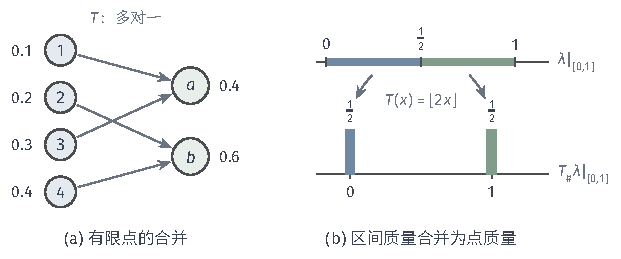
\includegraphics[width=105.1mm]{figures/02-abstract-mathematics/01-metric-and-measure/tikz/c2-pushforward-merge/figure.pdf}
  \caption{推前测度累计原像的质量。(a)四个带权点经多对一映射送到$a,b$两点，$a$收集点$1,3$的权重$0.1+0.3=0.4$，$b$收集点$2,4$的权重$0.2+0.4=0.6$；(b)$[0,1]$上的长度测度经$T(x)=\lfloor2x\rfloor$推前，原像$[0,\tfrac12)$与$[\tfrac12,1)$的长度分别汇集为点$0$和点$1$处的质量$\tfrac12$，单点$\{1\}$的长度为零，不贡献质量。}
  \label{fig:push-merge}
\end{figure}

\paragraph{平移与伸缩}
在实轴上，平移$T(x)=x+t$满足$T^{-1}(B)=B-t$，由Lebesgue测度的平移不变性，$T_\#\lambda=\lambda$；这种使$T_\#\mu=\mu$的映射称为\term{保持测度}（measure-preserving）的映射。伸缩则改变长度。令$T(x)=2x$，区间$(a,b]$的原像是$(a/2,b/2]$，所以$(T_\#\lambda)((a,b])=(b-a)/2$。两个测度$T_\#\lambda$与$\tfrac12\lambda$在全部半开区间上一致，并在每个$(-n,n]$上有限，由测度延拓的唯一性，$T_\#\lambda=\tfrac12\lambda$。把实轴拉长一倍，同一个输出区间只收集到原来一半长度的输入。这个例子将在第~\ref{sec:push-smooth-change}小节用来核对坐标换元中因子的方向。

\paragraph{坐标投影}
多元问题中最常见的多对一映射是坐标投影。设$\mu$是$\mathcal B(\mathbb R^d)$上的测度，$1\leq k<d$，$\pi(\bm x)=(x_1,\ldots,x_k)$。$\pi$连续，因而Borel可测，且对$B\in\mathcal B(\mathbb R^k)$有$\pi^{-1}(B)=B\times\mathbb R^{d-k}$，所以
\[
(\pi_\#\mu)(B)=\mu\bigl(B\times\mathbb R^{d-k}\bigr).
\]
$\pi_\#\mu$称为$\mu$在前$k$个坐标上的\term{边缘测度}（marginal measure）。它只回答形如“前$k$个坐标落在$B$中”的问题，保留的是$\mu$在柱形集合$B\times\mathbb R^{d-k}$上的值；后$d-k$个坐标怎样分布、两组坐标之间怎样关联，都不再能从边缘测度读出。概率论中由联合分布得到边缘分布正是这一操作，可参考\BookChapterRef{chap:random-vectors}{卷七“随机向量与联合分布”章}。

\begin{example}[点质量与单位正方形的投影]
\label{ex:push-projection}
在$\mathbb R^2$上取$\mu=0.2\,\delta_{(0,0)}+0.3\,\delta_{(0,1)}+0.5\,\delta_{(1,1)}$。第一坐标的投影$\pi_1$把$(0,0)$与$(0,1)$都送到$0$，所以$(\pi_1)_\#\mu=0.5\,\delta_0+0.5\,\delta_1$；第二坐标的投影把$(0,1)$与$(1,1)$都送到$1$，所以$(\pi_2)_\#\mu=0.2\,\delta_0+0.8\,\delta_1$。两个边缘测度合起来也不能恢复$\mu$：四个格点上的质量只要横向与纵向的合计相同，边缘就相同。例如$0.1\,\delta_{(0,0)}+0.1\,\delta_{(1,0)}+0.4\,\delta_{(0,1)}+0.4\,\delta_{(1,1)}$的两个边缘也是$0.5\,\delta_0+0.5\,\delta_1$与$0.2\,\delta_0+0.8\,\delta_1$，它却给$(1,0)$正质量。

再取$\nu=\lambda_2|_{[0,1]^2}$。对$B=(a,b]$，$\pi_1^{-1}(B)\cap[0,1]^2=((a,b]\cap[0,1])\times[0,1]$是一个矩形，面积等于$\lambda((a,b]\cap[0,1])$。于是$(\pi_1)_\#\nu$与$\lambda|_{[0,1]}$在全部半开区间上一致，总量都为$1$，由延拓的唯一性，二者相等。图~\ref{fig:push-projection}画出了两种情形。
\end{example}

\begin{figure}[!htbp]
  \centering
  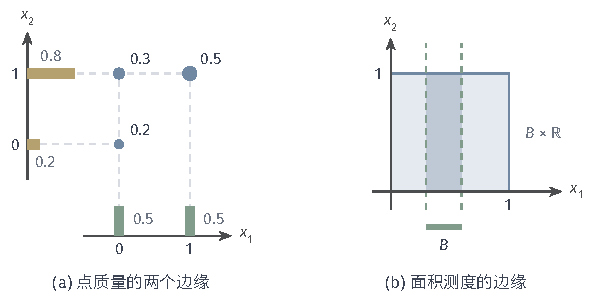
\includegraphics[width=100.9mm]{figures/02-abstract-mathematics/01-metric-and-measure/tikz/c2-projection-marginal/figure.pdf}
  \caption{坐标投影产生的边缘测度。(a)平面上三个点质量$0.2,0.3,0.5$，向横轴投影得到$0.5\delta_0+0.5\delta_1$，向纵轴投影得到$0.2\delta_0+0.8\delta_1$；(b)单位正方形上的面积测度，横轴区间$B$的边缘质量等于竖条$B\times\mathbb R$与正方形之交的面积，结果是$[0,1]$上的长度。}
  \label{fig:push-projection}
\end{figure}

边缘测度的总量与原测度相同，但$\sigma$有限性同样可能丢失：对整个平面上的$\lambda_2$，任一非退化区间$B$都有$(\pi_1)_\#\lambda_2(B)=\lambda_2(B\times\mathbb R)=+\infty$。上面的点质量例子还说明，输出测度不一定有密度，它可以是离散的。推前测度上的积分怎样计算，是下一节的问题；边缘测度何时有密度、怎样由原测度的密度算出，在第~\ref{sec:push-projection-density}小节处理。

\section{推前积分恒等式}
\label{sec:push-integral-identity}

上一节确定了目标空间上的质量。现在对目标空间上的函数$g$积分：$\int_Yg\,\mathrm d(T_\#\mu)$能否回到原空间计算？直观上，每个点$x$带着质量被送到$T(x)$，在那里读取函数值$g(T(x))$，所以应当有$\int_Yg\,\mathrm d(T_\#\mu)=\int_Xg\circ T\,\mathrm d\mu$。先对指示函数核对。若$g=\mathbf 1_B$，左端是$(T_\#\mu)(B)=\mu(T^{-1}(B))$；而$\mathbf 1_B(T(x))=1$当且仅当$x\in T^{-1}(B)$，即$\mathbf 1_B\circ T=\mathbf 1_{T^{-1}(B)}$，右端也等于$\mu(T^{-1}(B))$。沿积分的构造步骤推广，就得到一般结论。

\begin{theorem}[推前积分恒等式]
\label{thm:push-integral-identity}
设$(X,\mathcal A,\mu)$是测度空间，$T:(X,\mathcal A)\to(Y,\mathcal B)$可测。
\begin{enumerate}
\item 对每个可测$g:Y\to[0,+\infty]$，
\begin{equation}
\int_Yg\,\mathrm d(T_\#\mu)=\int_Xg\circ T\,\mathrm d\mu ,
\label{eq:push-integral-identity}
\end{equation}
两边可以同为$+\infty$。
\item 对可测的实值或复值$g$，$g$关于$T_\#\mu$可积当且仅当$g\circ T$关于$\mu$可积，此时式~\eqref{eq:push-integral-identity}成立且两边有限。
\end{enumerate}
\end{theorem}

\begin{proof}
$g\circ T$是可测映射的复合，因而可测。(1) 指示函数的情形已在上面核对。对非负简单函数$s=\sum_ic_i\mathbf 1_{B_i}$，$s\circ T=\sum_ic_i\mathbf 1_{B_i}\circ T$，两边由线性性相等。对一般非负可测$g$，取非负简单函数$s_n\uparrow g$，则$s_n\circ T\uparrow g\circ T$，两边分别用单调收敛定理取极限。

(2) 由$\lvert g\circ T\rvert=\lvert g\rvert\circ T$，把(1)用于$\lvert g\rvert$，两边的绝对积分相等，可积性等价。实值时$(g\circ T)^\pm=g^\pm\circ T$，对正部和负部分别用(1)后相减，两边都是有限数之差；复值时对实部和虚部分别处理。
\end{proof}

定理只用到可测性与推前测度的定义。它不要求$T$可逆或可微，不要求$X,Y$有距离或坐标，也不要求$T_\#\mu$相对于任何参考测度有密度。这里沿映射转移的是测度，被积函数相应地复合上$T$；这与上一章的换测度公式不同，那里点不移动，被积函数不变，只是累计权重乘上密度。

恒等式可以从两个方向读。已知$\mu$时，它把目标空间上的积分化为原空间上的积分，例如随机变量的函数的期望，可以直接在原来的概率空间上计算，不必先求出输出的分布。反过来，它说明对复合函数$g\circ T$的累计只取决于$T$把质量送到了哪里：两个映射若推前出同一个测度，所有形如$\int g\circ T\,\mathrm d\mu$的积分都相同。

\begin{example}[有限集合上的分组汇总]
\label{ex:push-finite-sum}
取$X=\{1,2,3,4\}$，$\mu(\{k\})=k/10$；$Y=\{0,1\}$，$T(1)=T(3)=1$，$T(2)=T(4)=0$。输出点$0$的原像是$\{2,4\}$，所以$(T_\#\mu)(\{0\})=0.2+0.4=0.6$；同理$(T_\#\mu)(\{1\})=0.1+0.3=0.4$。取$g(0)=5$、$g(1)=2$，左端是$5\times0.6+2\times0.4=3.8$；右端逐个原像点计算$g(T(k))\mu(\{k\})$，得$2\times0.1+5\times0.2+2\times0.3+5\times0.4=3.8$。
\end{example}

图~\ref{fig:push-finite-sum}显示了两种算法的差别：右端逐点累计，左端先把映到同一输出点的质量合并，再乘以该点的函数值。整个计算没有用到任何“输出密度”，输出测度本身就是两个原子。

\begin{figure}[!htbp]
\centering
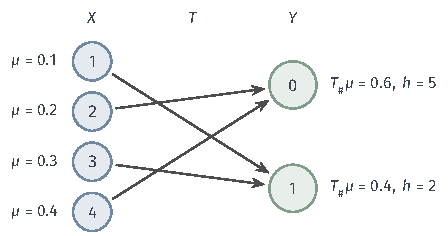
\includegraphics[width=75.812mm]{figures/02-abstract-mathematics/01-metric-and-measure/tikz/c3-pushforward-change/figure.pdf}
\caption{有限集合上的推前与换元。输入点$k=1,2,3,4$的质量为$k/10$，映射$T$把$2,4$送到$0$、把$1,3$送到$1$，输出质量分别为$0.6$与$0.4$。取$h(0)=5$、$h(1)=2$（正文记作$g$），按输出点汇总与按输入点逐个累计都得到$3.8$。}
\label{fig:push-finite-sum}
\end{figure}

\paragraph{连续情形与复合}
在$[0,1]$上取$\mu=\lambda|_{[0,1]}$，$T(x)=\lfloor2x\rfloor$，上一节已求出$T_\#\mu=\tfrac12\delta_0+\tfrac12\delta_1$。对$g(y)=y^2+1$，左端$\tfrac12g(0)+\tfrac12g(1)=\tfrac12+1=\tfrac32$；右端$\int_0^1(\lfloor2x\rfloor^2+1)\,\mathrm dx=\int_0^{1/2}1\,\mathrm dx+\int_{1/2}^12\,\mathrm dx=\tfrac32$，单点$x=1$不影响积分。若接着再作映射$S:Y\to Z$，由$(S\circ T)_\#\mu=S_\#(T_\#\mu)$，式~\eqref{eq:push-integral-identity}可以逐级使用：$\int_Zk\,\mathrm d((S\circ T)_\#\mu)=\int_Yk\circ S\,\mathrm d(T_\#\mu)=\int_Xk\circ S\circ T\,\mathrm d\mu$。

\paragraph{可积性条件}
第2条中的可积性条件不能省。在$(0,1)$上取$\mu=\lambda|_{(0,1)}$，$T(x)=1/x$，把质量送到$(1,\infty)$。对$g(y)=\sin y$，$\int_{(0,1)}\lvert\sin(1/x)\rvert\,\mathrm dx\leq1$，两边都可积，恒等式成立。对$g(y)=y$，$\int_0^1(1/x)\,\mathrm dx=+\infty$，按第1条两边同为$+\infty$，仍是一个正确的等式；但若换成带符号的$g(y)=y\sin y$，可以验证两边的正部与负部积分都是$+\infty$，这时式~\eqref{eq:push-integral-identity}没有意义，而不是不成立。实际使用时，应先对$\lvert g\rvert$用第1条确认可积，再写出有符号的等式。

\section{映射后的密度}
\label{sec:push-mapped-densities}

推前积分恒等式把目标空间上的积分送回原空间。但在目标空间上直接计算时，我们往往希望把推前测度写成一个熟悉的参考测度的加权形式，就像在实轴上用概率密度代替分布本身。

设在目标空间$Y$上选定参考测度$\lambda$，并假设推前测度有密度
\[
h=\frac{\mathrm d(T_\#\mu)}{\mathrm d\lambda}.
\]
对非负可测$g$，连续使用推前积分恒等式与第~\ref{chap:measure-densities}章的换测度公式，得到两步改写
\begin{equation}
\int_Xg\circ T\,\mathrm d\mu=\int_Yg\,\mathrm d(T_\#\mu)=\int_Ygh\,\mathrm d\lambda .
\label{eq:push-two-step}
\end{equation}

第一步沿映射转移测度并复合被积函数，第二步留在$Y$上，只把累计权重换成$h$。两步依据不同的定理，条件也不同：第一步对任何可测映射成立，第二步要求密度存在。

\paragraph{密度未必存在}
密度存在的必要条件是$T_\#\mu\ll\lambda$，即对每个$\lambda$零测集$N\subset Y$，都有
\[
\mu\bigl(T^{-1}(N)\bigr)=0 .
\]
也就是说，映射不能把正的质量压进目标空间的零测集。

常值映射给出最简单的反例。令$X=[0,1]$，$\mu=\lambda|_{[0,1]}$，$T(x)=c$。当$c\in B$时$T^{-1}(B)=[0,1]$，否则$T^{-1}(B)=\varnothing$，所以
\[
T_\#\mu=\delta_c .
\]
单点$\{c\}$是Lebesgue零测集，却承载全部质量，$T_\#\mu$与$\lambda$相互奇异，没有Lebesgue密度。映射把一段区间压成一点，原像$T^{-1}(\{c\})$有正长度，这就是失败的原因。

所以计算映射后的密度，要先确认映射不把正质量压进零测集。下面三个小节分别处理三种常见结构：光滑可逆映射、分成有限个可逆光滑分支的映射，以及坐标投影。

\subsection{光滑坐标换元}
\label{sec:push-smooth-change}

设$U,V\subset\mathbb R^d$是开集。若$T:U\to V$是双射，$T$与$T^{-1}$都连续可微，就称$T$为$C^1$\term{微分同胚}（diffeomorphism）。对$T^{-1}\circ T=\mathrm{id}$求导，得
\[
DT^{-1}\bigl(T(\bm x)\bigr)\,DT(\bm x)=\bm I .
\]

取行列式可知\term{Jacobian行列式}（Jacobian determinant）$\det DT(\bm x)$处处不为零，并且
\begin{equation}
\bigl\lvert\det DT^{-1}(\bm y)\bigr\rvert=\frac{1}{\bigl\lvert\det DT\bigl(T^{-1}(\bm y)\bigr)\bigr\rvert},\qquad\bm y\in V .
\label{eq:push-inverse-jacobian}
\end{equation}
本小节记$S=T^{-1}:V\to U$，它也是$C^1$微分同胚。所有函数与集合都取Borel可测的版本。

\paragraph{Lebesgue测度的推前}
先以$\lambda_d|_U$为原测度，问它推前到$V$上是什么。由定义，小盒子$Q\subset V$得到的质量是它的原像$S(Q)$的体积。$S$在小盒子上近似于线性映射$DS(\bm y)$，线性映射把体积乘以行列式的绝对值，所以
\[
(T_\#\lambda_d)(Q)=\lambda_d\bigl(S(Q)\bigr)\approx\bigl\lvert\det DS(\bm y)\bigr\rvert\,\lambda_d(Q).
\]
这说明推前测度的密度应当是逆映射的Jacobian因子。

用极坐标算一个具体的小盒子。取$S(r,\theta)=(r\cos\theta,r\sin\theta)$，$T$是它的逆，Jacobian行列式为
\[
\det DS(r,\theta)=r .
\]
取$Q=[1,1.2]\times[0.3,0.8]$，它的面积是$0.2\times0.5=0.1$。它的原像$S(Q)$是一块环形扇区，面积是
\[
\lambda_2\bigl(S(Q)\bigr)=\int_{0.3}^{0.8}\int_1^{1.2}r\,\mathrm dr\,\mathrm d\theta=0.5\times\frac{1.2^2-1^2}{2}=0.11 .
\]

两个面积之比是$0.11/0.1=1.1$，恰好是$Q$中心$r=1.1$处的$\lvert\det DS\rvert$。图~\ref{fig:push-local-volume}画出了这个小盒子和它的原像。绿色虚线是线性化$DS$给出的平行四边形，面积也是$1.1\times0.1=0.11$；它与真实的环形扇区只差一些边角，盒子越小差得越少。

\begin{BookInlineFigure}
  \centering
  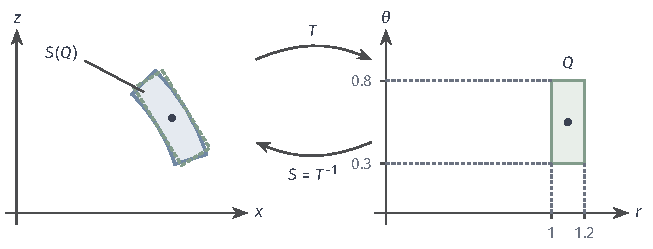
\includegraphics[width=110.539mm]{figures/04-spaces-measures-and-geometry/02-measure/tikz/push-local-volume/figure.pdf}
  \caption{小盒子的原像决定局部密度。右图是极坐标平面上的盒子$Q=[1,1.2]\times[0.3,0.8]$，左图蓝色区域是它在$(x,z)$平面的原像$S(Q)$，绿色虚线是中心处线性化$DS$给出的平行四边形，黑点是中心。两张图用相同的比例尺，面积分别为$0.1$与$0.11$，比值$1.1$等于$\lvert\det DS\rvert$在中心的值。}
  \label{fig:push-local-volume}
\end{BookInlineFigure}

把这个局部比例严格化，需要卷二的经典换元公式。设$E\subset V$是紧Jordan区域，$S(E)$也是Jordan区域，$f$在$S(E)$上连续，则
\begin{equation}
\int_{S(E)}f(\bm x)\,\mathrm d\bm x=\int_Ef\bigl(S(\bm y)\bigr)\,\lvert\det DS(\bm y)\rvert\,\mathrm d\bm y .
\label{eq:push-classical-change}
\end{equation}
公式的陈述和证明思路见\BookChapterRef{chap:region-integrals}{卷二第24章“区域积分”}。证明需要对细分作一致的误差控制，篇幅较长，读者可查阅实分析教材。我们只用它在闭盒子上、$f\equiv1$时的情形，再用测度延拓的唯一性推广到一切Borel集。

\begin{theorem}[微分同胚下Lebesgue测度的推前]
\label{thm:push-lebesgue-diffeo}
设$T:U\to V$是$C^1$微分同胚。则对每个Borel集$B\subset V$，
\begin{equation}
(T_\#\lambda_d)(B)=\lambda_d\bigl(T^{-1}(B)\bigr)=\int_B\bigl\lvert\det DT^{-1}(\bm y)\bigr\rvert\,\mathrm d\bm y ,
\label{eq:push-lebesgue-diffeo}
\end{equation}
即$T_\#(\lambda_d|_U)$相对于$\lambda_d|_V$的密度是$\lvert\det DT^{-1}\rvert$。
\end{theorem}

\begin{proof}
令$\nu(B)=\int_B\lvert\det DS\rvert\,\mathrm d\bm y$，它是$V$的Borel集上的测度。证明分两步：先在闭盒子上比较$T_\#\lambda_d$与$\nu$，再推广到全部Borel集。

设$Q\subset V$是闭盒子，允许退化。$S$是同胚，所以$S(Q)$是紧集，边界是$S(\partial Q)$。$S$在凸紧集$Q$上连续可微，由中值不等式在$Q$上Lipschitz，因而把$Q$中容量为零的集合映成容量为零的集合。$\partial Q$的容量为零，所以$S(\partial Q)$的容量为零，$S(Q)$是紧Jordan区域。

对$E=Q$、$f\equiv1$用式~\eqref{eq:push-classical-change}。Jordan区域上连续函数的Riemann积分等于Lebesgue积分，于是
\[
(T_\#\lambda_d)(Q)=\lambda_d\bigl(S(Q)\bigr)=\int_Q\lvert\det DS(\bm y)\rvert\,\mathrm d\bm y=\nu(Q).
\]

含于$V$的闭盒子连同空集对有限交封闭，构成$\pi$系统。$V$的每个开子集都是可数个含于其中的有理端点闭盒子之并，所以这些盒子生成$V$上的Borel $\sigma$代数，并有可数个覆盖$V$。两个测度在每个闭盒子上都有限，因为$S(Q)$紧、$\lvert\det DS\rvert$在$Q$上有界。由第~\ref{chap:measure}章的延拓唯一性，$T_\#\lambda_d=\nu$在$V$的全部Borel集上成立。
\end{proof}

定理说明，推前测度的密度在新坐标$\bm y$处取值，因子是逆映射的Jacobian。由式~\eqref{eq:push-inverse-jacobian}，它也可以写成$1/\lvert\det DT(S(\bm y))\rvert$：$T$在原像附近把体积拉伸的地方，同样多的质量摊到更大的范围，密度就变小。

\paragraph{原测度有密度的情形}
现在设$U$上的测度$\mu$相对于$\lambda_d$有密度$p$。把推前积分恒等式、换测度公式与上一个定理接起来，就得到推前测度的密度。

\begin{theorem}[微分同胚下的推前密度]
\label{thm:push-density-diffeo}
设$T:U\to V$是$C^1$微分同胚，$U$上的测度$\mu$相对于$\lambda_d$有密度$p$。则$T_\#\mu$相对于$V$上的$\lambda_d$有密度
\begin{equation}
q(\bm y)=p\bigl(T^{-1}(\bm y)\bigr)\,\bigl\lvert\det DT^{-1}(\bm y)\bigr\rvert ,\qquad\bm y\in V .
\label{eq:push-density-diffeo}
\end{equation}
\end{theorem}

\begin{proof}
设$B\subset V$是Borel集。由推前测度和密度的定义，
\[
(T_\#\mu)(B)=\mu\bigl(T^{-1}(B)\bigr)=\int_U\mathbf 1_B\bigl(T(\bm x)\bigr)\,p(\bm x)\,\mathrm d\bm x .
\]

因为$\bm x=S(T(\bm x))$，被积函数可以写成$\psi\circ T$，其中
\[
\psi(\bm y)=\mathbf 1_B(\bm y)\,p\bigl(S(\bm y)\bigr)
\]
是$V$上的非负Borel函数。对$\lambda_d|_U$与$T$用推前积分恒等式，再用定理~\ref{thm:push-lebesgue-diffeo}的密度与换测度公式，得到
\[
\begin{aligned}
\int_U\psi\circ T\,\mathrm d\lambda_d&=\int_V\psi\,\mathrm d(T_\#\lambda_d)\\
&=\int_V\psi(\bm y)\,\lvert\det DS(\bm y)\rvert\,\mathrm d\bm y\\
&=\int_Bp\bigl(S(\bm y)\bigr)\,\lvert\det DS(\bm y)\rvert\,\mathrm d\bm y .
\end{aligned}
\]
这正是$(T_\#\mu)(B)=\int_Bq\,\mathrm d\lambda_d$。
\end{proof}

\paragraph{与通常换元公式对照}
通常的积分换元公式中出现的是正向的Jacobian，这与定理~\ref{thm:push-density-diffeo}的因子方向相反。它也可以由定理~\ref{thm:push-lebesgue-diffeo}得到：把定理用于微分同胚$S:V\to U$，得到$S_\#\lambda_d$的密度是$\lvert\det DS^{-1}\rvert=\lvert\det DT\rvert$。

对非负Borel函数$g$，把$g$写成$(g\circ T)\circ S$，用推前积分恒等式，再用这个密度，得到
\begin{equation}
\begin{aligned}
\int_Vg\,\mathrm d\lambda_d&=\int_V(g\circ T)\circ S\,\mathrm d\lambda_d\\
&=\int_Ug\circ T\,\mathrm d(S_\#\lambda_d)\\
&=\int_Ug\bigl(T(\bm x)\bigr)\,\lvert\det DT(\bm x)\rvert\,\mathrm d\bm x .
\end{aligned}
\label{eq:push-jacobian-change}
\end{equation}

两个公式回答不同的问题。式~\eqref{eq:push-density-diffeo}问的是“新坐标$\bm y$处每单位体积有多少质量”，所以因子在新坐标上取值，是逆映射的Jacobian。式~\eqref{eq:push-jacobian-change}把新坐标上的体积元改写到原坐标上，所以因子在原坐标上取值，是正向映射的Jacobian。

用第~\ref{sec:push-mass-transfer}小节的伸缩$T(x)=2x$核对方向。这时$T^{-1}(y)=y/2$，导数的绝对值是$\tfrac12$，由定理~\ref{thm:push-lebesgue-diffeo}，
\[
T_\#\lambda=\tfrac12\lambda ,
\]
与按原像直接计算的结果一致：拉长一倍，密度减半。

而式~\eqref{eq:push-jacobian-change}给出
\[
\int g(y)\,\mathrm dy=\int g(2x)\cdot2\,\mathrm dx ,
\]
因子是正向导数$T'=2$：原坐标的一小段$\mathrm dx$，在新坐标中长$2\,\mathrm dx$。把两个因子混用，密度会算成实际值的四倍或四分之一。

\begin{example}[指数分布与仿射变换]
\label{ex:push-exponential}
取$(0,1)$上的均匀概率测度，密度$p=1$，经$T(x)=-\ln x$映到$(0,+\infty)$。逆映射与导数分别是
\[
T^{-1}(y)=\mathrm e^{-y},\qquad\bigl\lvert(T^{-1})'(y)\bigr\rvert=\mathrm e^{-y}.
\]

由式~\eqref{eq:push-density-diffeo}，输出密度是
\[
q(y)=\mathrm e^{-y},\qquad y>0 ,
\]
这是指数分布，总质量$\int_0^\infty\mathrm e^{-y}\,\mathrm dy=1$。

核对一个集合。$(1,2]$的原像是$[\mathrm e^{-2},\mathrm e^{-1})$，于是
\[
(T_\#\mu)\bigl((1,2]\bigr)=\mathrm e^{-1}-\mathrm e^{-2}=\int_1^2\mathrm e^{-y}\,\mathrm dy .
\]

再看仿射变换$T(\bm x)=\bm A\bm x+\bm b$，其中$\bm A$可逆。逆映射是$\bm A^{-1}(\bm y-\bm b)$，Jacobian因子是常数$1/\lvert\det\bm A\rvert$，所以
\[
q(\bm y)=\frac{p\bigl(\bm A^{-1}(\bm y-\bm b)\bigr)}{\lvert\det\bm A\rvert}.
\]
\end{example}

图~\ref{fig:push-exponential-bins}把指数分布例子中的密度“算”了出来。把$(0,1)$分成长度$0.2$的小段，每段质量都是$0.2$。靠近$x=1$的小段$(0.8,1)$映到长度约$0.223$的区间，平均高度约$0.2/0.223\approx0.90$；$(0.2,0.4]$映到长度约$0.693$的区间，平均高度约$0.29$。$T$拉得越长的地方，矩形越矮，这些矩形的高度沿着$\mathrm e^{-y}$下降。

\begin{BookInlineFigure}
  \centering
  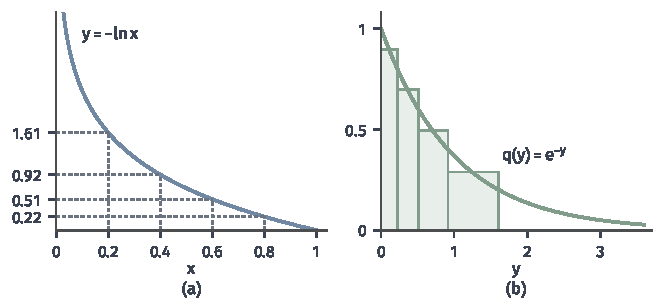
\includegraphics[width=112mm]{figures/04-spaces-measures-and-geometry/02-measure/matplotlib/push-exponential-bins/figure.pdf}
  \caption{由等质量分割看推前密度。(a)映射$y=-\ln x$与$x=0.2,0.4,0.6,0.8$对应的$y$值。(b)绿色矩形的底是长度$0.2$的输入小段映成的区间，面积都是$0.2$，所以高度等于$0.2$除以区间长度；曲线是极限密度$q(y)=\mathrm e^{-y}$。最左的输入小段$(0,0.2]$映到$[1.61,+\infty)$，质量$0.2$落在右侧的尾部，图中未画矩形。}
  \label{fig:push-exponential-bins}
\end{BookInlineFigure}

\subsection{多分支映射}
\label{sec:push-branches}

许多映射不是整体可逆的。$T(x)=x^2$把$x$与$-x$送到同一点，但在$(0,1)$与$(-1,0)$上分别是微分同胚。这类映射的处理办法是把定义域分成几块，在每块上用上一小节的公式，再把落到同一目标点的贡献加起来。

\begin{theorem}[分支映射的推前密度]
\label{thm:push-branch-density}
设$U\subset\mathbb R^d$是开集，$U_1,\ldots,U_m\subset U$是两两不交的开集，例外集$E=U\setminus\bigcup_kU_k$是Lebesgue零测集。设$T:U\to\mathbb R^d$可测，并且每个限制$T_k=T|_{U_k}$是$U_k$到开集$V_k=T(U_k)$的$C^1$微分同胚，$S_k=T_k^{-1}$。若$U$上的测度$\mu$相对于$\lambda_d$有密度$p$，则$T_\#\mu$相对于$\lambda_d$有密度
\begin{equation}
q(\bm y)=\sum_{k=1}^m\mathbf 1_{V_k}(\bm y)\,p\bigl(S_k(\bm y)\bigr)\,\bigl\lvert\det DS_k(\bm y)\bigr\rvert .
\label{eq:push-branch-density}
\end{equation}
\end{theorem}

\begin{proof}
对Borel集$B\subset\mathbb R^d$，把原像按分支拆开，
\[
T^{-1}(B)=\bigl(T^{-1}(B)\cap E\bigr)\cup\bigcup_{k=1}^m\bigl(T^{-1}(B)\cap U_k\bigr),
\]
各部分两两不交。$\mu\ll\lambda_d$，所以$\mu(E)=0$，第一部分不贡献质量。

在第$k$块上，$T^{-1}(B)\cap U_k=T_k^{-1}(B\cap V_k)$。把定理~\ref{thm:push-density-diffeo}用于$T_k$与$U_k$上的测度$\mu|_{U_k}$，其密度是$p$在$U_k$上的限制，得到
\[
\mu\bigl(T_k^{-1}(B\cap V_k)\bigr)=\int_{B\cap V_k}p\bigl(S_k(\bm y)\bigr)\,\lvert\det DS_k(\bm y)\rvert\,\mathrm d\bm y .
\]

对$k$求和，有限个非负积分之和等于和的积分，于是$(T_\#\mu)(B)=\int_Bq\,\mathrm d\lambda_d$。
\end{proof}

定理的三个条件各管一件事。分支两两不交，保证每个原像点只计算一次。例外集$E$是零测集，保证没有遗漏质量；若$T$在一段正长度的区间上取常值，这段不能纳入任何分支，那里可能产生原子，必须另行计算。

各分支的像$V_k$可以重叠。重叠处的点有多个原像，每个原像所在的分支都贡献一项，所以要求和；只取一个逆分支会漏掉其余原像处的质量。可数个分支的情形也成立，此时交换求和与积分的依据是单调收敛定理。

\begin{example}[平方映射]
\label{ex:push-square}
取$[-1,1]$上的均匀概率测度，密度$p=\tfrac12$，$T(x)=x^2$。端点的质量为零，取$U=(-1,1)$。两个分支是$U_1=(0,1)$与$U_2=(-1,0)$，例外集$E=\{0\}$是零测集；两支的像都是$(0,1)$，逆映射分别是
\[
S_1(y)=\sqrt y,\qquad S_2(y)=-\sqrt y ,
\]
导数的绝对值都是$1/(2\sqrt y)$。由式~\eqref{eq:push-branch-density}，在$0<y<1$上
\[
q(y)=\frac12\cdot\frac{1}{2\sqrt y}+\frac12\cdot\frac{1}{2\sqrt y}=\frac{1}{2\sqrt y},
\]
在$(0,1)$外$q=0$。总质量是
\[
\int_0^1\frac{\mathrm dy}{2\sqrt y}=\bigl[\sqrt y\bigr]_0^1=1 .
\]

核对一个集合。取$B=[0.36,0.49]$，原像是$[-0.7,-0.6]\cup[0.6,0.7]$，总长度$0.2$，输入质量是
\[
0.2\times\tfrac12=0.1 .
\]
用输出密度计算，
\[
\int_{0.36}^{0.49}\frac{\mathrm dy}{2\sqrt y}=0.7-0.6=0.1 .
\]
若只取正分支，得到的$1/(4\sqrt y)$总积分只有$\tfrac12$，漏掉了另一半质量。
\end{example}

图~\ref{fig:push-square}左侧显示了例子中的计算：黄色带是输出区间$B$，它在曲线上碰到两个分支，往下落到两段蓝色的输入区间，各贡献质量$0.05$。右侧是相加后的密度，虚线是只取一个分支时的结果。

\begin{BookInlineFigure}
  \centering
  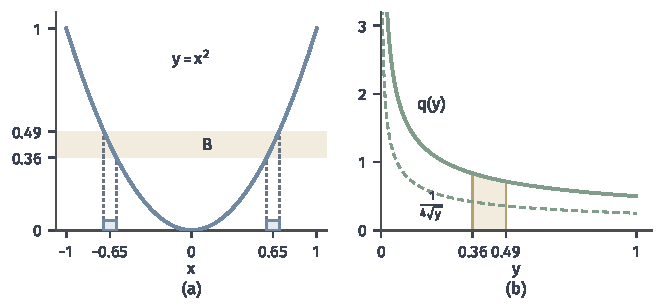
\includegraphics[width=112mm]{figures/04-spaces-measures-and-geometry/02-measure/matplotlib/push-square/figure.pdf}
  \caption{平方映射的推前密度。(a)映射$y=x^2$；输出区间$B=[0.36,0.49]$（黄色带）有两个原像$[-0.7,-0.6]$与$[0.6,0.7]$（蓝色）。(b)实线是两支相加的密度$q(y)=1/(2\sqrt y)$，虚线是只取一个分支的$1/(4\sqrt y)$；$B$上实线下的面积是$0.1$，与输入质量一致。纵轴在$3.2$处截断，$y\to0$时$q$无界但可积。}
  \label{fig:push-square}
\end{BookInlineFigure}

输出密度在$y\to0$时无界，但仍可积。原点的原像只有单点$\{0\}$，输入质量为$0$，所以输出没有点质量。若输入在$0$处有点质量，例如换成$\tfrac12\delta_0+\tfrac14\lambda|_{[-1,1]}$，原测度就不再相对于$\lambda$绝对连续，定理不适用；推前后在$0$处出现点质量$\tfrac12$，这部分不能用相对于长度的密度表示。

\subsection{坐标投影}
\label{sec:push-projection-density}

坐标投影也是多对一映射，但与上一小节不同：落到同一点$x_1$的原像不是有限个点，而是整条\term{纤维}（fiber）$\{x_1\}\times X_2$，其上每一点的质量通常为零。有限分支求和在这里无从谈起，应当沿纤维积分。为此需要原测度相对于乘积参考测度有密度。

\begin{theorem}[边缘密度]
\label{thm:push-marginal-density}
设$(X_1,\mathcal A_1,\mu_1)$与$(X_2,\mathcal A_2,\mu_2)$是$\sigma$有限测度空间，$X_1\times X_2$上的测度$\mu$相对于乘积测度$\mu_1\otimes\mu_2$有密度$p$，$\pi(x_1,x_2)=x_1$。则$\pi_\#\mu$相对于$\mu_1$有密度
\begin{equation}
p_1(x_1)=\int_{X_2}p(x_1,x_2)\,\mu_2(\mathrm dx_2).
\label{eq:push-marginal-density}
\end{equation}
\end{theorem}

\begin{proof}
对$B\in\mathcal A_1$，原像是$\pi^{-1}(B)=B\times X_2$。由密度的定义，再对非负函数用Tonelli定理，
\[
\begin{aligned}
(\pi_\#\mu)(B)&=\mu(B\times X_2)\\
&=\int_{X_1\times X_2}\mathbf 1_B(x_1)\,p(x_1,x_2)\,\mathrm d(\mu_1\otimes\mu_2)\\
&=\int_B\Bigl(\int_{X_2}p(x_1,x_2)\,\mu_2(\mathrm dx_2)\Bigr)\mu_1(\mathrm dx_1).
\end{aligned}
\]
Tonelli定理同时保证内层积分$p_1$是$x_1$的可测函数。于是$(\pi_\#\mu)(B)=\int_Bp_1\,\mathrm d\mu_1$。
\end{proof}

$p_1$取值于$[0,+\infty]$。若$\mu$有限，取$B=X_1$得
\[
\int_{X_1}p_1\,\mathrm d\mu_1=\mu(X_1\times X_2)<+\infty ,
\]
所以$p_1$在$\mu_1$几乎处处有限。

被积函数非负，用Tonelli定理就够了；若要对有符号的$g(x_1)$计算$\int g\,\mathrm d(\pi_\#\mu)$，则要先确认$\int\lvert g\rvert p_1\,\mathrm d\mu_1<+\infty$，这时Fubini定理保证换序。

参考测度取计数测度时，式~\eqref{eq:push-marginal-density}中的积分变成对第二个坐标求和，就是离散联合分布求边缘的公式，也就是图~\ref{fig:push-projection}中逐行逐列的合计。

\begin{example}[正方形上的线性密度]
\label{ex:push-square-marginal}
在$[0,1]^2$上取$\mu$相对于$\lambda_2$的密度$p(x,z)=x+z$。总质量是
\[
\int_0^1\!\!\int_0^1(x+z)\,\mathrm dz\,\mathrm dx=\int_0^1\bigl(x+\tfrac12\bigr)\,\mathrm dx=1 .
\]

第一坐标的边缘密度由式~\eqref{eq:push-marginal-density}算出：
\[
p_1(x)=\int_0^1(x+z)\,\mathrm dz=x+\tfrac12,\qquad0\leq x\leq1 .
\]

核对一个集合。用边缘密度计算，
\[
(\pi_\#\mu)\bigl([0,\tfrac12]\bigr)=\int_0^{1/2}\bigl(x+\tfrac12\bigr)\,\mathrm dx=\tfrac18+\tfrac14=\tfrac38 .
\]
直接用原测度计算，
\[
\mu\bigl([0,\tfrac12]\times[0,1]\bigr)=\int_0^{1/2}\!\!\int_0^1(x+z)\,\mathrm dz\,\mathrm dx=\tfrac38 ,
\]
两者相同。
\end{example}

图~\ref{fig:push-marginal-fiber}把例子中的一条纤维单独取出来。在$x=0.3$处，纤维是竖直的线段，密度沿纤维是$0.3+z$，积分得到$0.3+\tfrac12=0.8$，这就是$p_1(0.3)$。对每个$x$做一次这样的积分，$p_1$的整条曲线就出来了。

\begin{BookInlineFigure}
  \centering
  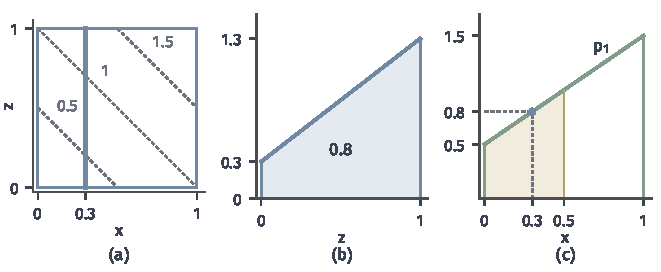
\includegraphics[width=112mm]{figures/04-spaces-measures-and-geometry/02-measure/matplotlib/push-marginal-fiber/figure.pdf}
  \caption{沿纤维积分得到边缘密度。(a)单位正方形上$p(x,z)=x+z$的等值线（虚线，数字是$p$的值），粗线是$x=0.3$处的纤维。(b)沿这条纤维的密度$0.3+z$，阴影面积$0.8$。(c)边缘密度$p_1(x)=x+\tfrac12$，蓝点是(b)算出的值，黄色面积是$[0,\tfrac12]$上的质量$\tfrac38$。}
  \label{fig:push-marginal-fiber}
\end{BookInlineFigure}

\paragraph{与分支求和的区别}
投影与分支映射都是多对一的，但累计方式不同。分支映射的每个目标点只有有限个原像，每个原像附近映射是局部微分同胚，贡献由Jacobian因子换算后相加。投影的原像是整条纤维，纤维上单点没有质量，贡献必须用纤维上的参考测度$\mu_2$积分。表~\ref{tab:push-mechanisms}汇总了本节的三种机制。

\begin{BookInlineTable}
  \centering
  \begin{tabular}{@{}llll@{}}
    \toprule
    & 微分同胚 & 多分支映射 & 坐标投影\\
    \midrule
    目标点的原像 & 一个点 & 有限个点 & 一条纤维\\
    参考测度 & Lebesgue测度 & Lebesgue测度 & 乘积测度\\
    密度的来源 & 逆映射Jacobian & 各分支相加 & 沿纤维积分\\
    依据 & 经典换元公式 & 逐分支换元 & Tonelli定理\\
    \bottomrule
  \end{tabular}
  \caption{三种计算推前密度的机制。}
  \label{tab:push-mechanisms}
\end{BookInlineTable}

累次积分的依据是乘积结构：$\mu$的参考测度是乘积测度，纤维恰好是坐标截面。一般的非线性降维没有现成的乘积结构，必须另行核对沿纤维积分的条件，以及纤维上用什么参考测度。一种可行的做法是先用微分同胚把纤维拉直成坐标截面，再投影。

以单位圆盘$D$上的均匀概率测度为例，密度是$1/\pi$，映射$R(x,z)=\sqrt{x^2+z^2}$把点送到它到原点的距离，纤维是同心圆周。为把圆周拉直，先去掉零测的射线$\{(x,0):x\geq0\}$，此后极坐标
\[
\Phi(r,\theta)=(r\cos\theta,r\sin\theta)
\]
是$G=(0,1)\times(0,2\pi)$到圆盘剩余部分的微分同胚，Jacobian行列式是$r$。

令$T=\Phi^{-1}$，由式~\eqref{eq:push-density-diffeo}，$T_\#\mu$相对于$G$上面积的密度是
\[
q(r,\theta)=\frac1\pi\cdot r=\frac r\pi .
\]
$R$就是$T$与第一坐标投影$\pi_1$的复合，由复合规则~\eqref{eq:push-composition}和定理~\ref{thm:push-marginal-density}，半径的密度是
\[
p_R(r)=\int_0^{2\pi}\frac r\pi\,\mathrm d\theta=2r,\qquad0<r<1 .
\]

核对一个集合：半径不超过$s$的质量是面积比$s^2$，而$\int_0^s2r\,\mathrm dr=s^2$。图~\ref{fig:push-polar-fibers}中的黄色环带取$0.5<r\leq0.6$，三幅图里的质量都是$0.6^2-0.5^2=0.11$。

\begin{BookInlineFigure}
  \centering
  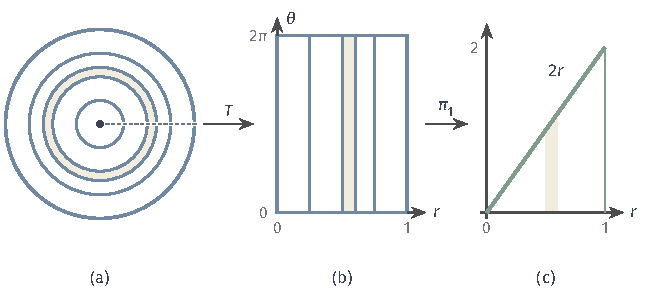
\includegraphics[width=109.813mm]{figures/04-spaces-measures-and-geometry/02-measure/tikz/push-polar-fibers/figure.pdf}
  \caption{先把纤维拉直再投影。(a)单位圆盘上$R(x,z)=\sqrt{x^2+z^2}$的几条纤维（同心圆周），虚线是去掉的射线。(b)极坐标平面上，同一批纤维变成竖直线段。(c)对$\theta$积分后得到半径的密度$2r$。黄色部分是$0.5<r\leq0.6$的同一批点，质量都是$0.11$。}
  \label{fig:push-polar-fibers}
\end{BookInlineFigure}

这个例子说明纤维上的参考测度不能想当然。直接对$\theta$积分平面密度$1/\pi$，得到常数$2$，总质量变成$2$，这是漏掉了Jacobian因子$r$。沿圆周用弧长积分$1/\pi$，得到$2\pi r/\pi=2r$，结果正确；但这个正确是有条件的。

换一个输出函数$t=x^2+z^2$，纤维还是同样的圆周。由半径的密度$2r$和映射$r\mapsto r^2$，用式~\eqref{eq:push-density-diffeo}，$t$的密度是
\[
2\sqrt t\cdot\frac{1}{2\sqrt t}=1,\qquad0<t<1 .
\]
这时沿圆周用弧长积分$1/\pi$仍然得到$2\sqrt t$，它在$(0,1)$上的总积分是$\tfrac43$，并不是$1$。

差别来自相邻两条纤维之间的距离。半径增加$\mathrm dr$时，相邻圆周的间距恰好是$\mathrm dr$；$t$增加$\mathrm dt$时，间距是$\mathrm dt/(2\sqrt t)$，所以弧长积分还要乘这个因子。同一族纤维，输出函数不同，纤维上应当使用的权重也不同，这就是一般降维必须单独核对的内容。

\section{本章小结}
\label{sec:push-summary}

本章开头问：原空间上的质量经可测映射后怎样分布在目标空间上，目标空间上的积分怎样回到原空间计算。第一个问题由原像回答。推前测度$T_\#\mu(B)=\mu(T^{-1}(B))$把目标集合的质量规定为它的原像的质量；原像保持不交并，所以推前测度可数可加，总质量不变，并且分步推前与一次推前相同。$\sigma$有限性则可能在推前时丢失，用到相关定理时要单独核对。

例子显示了推前测度记录什么、丢掉什么。一一映射只搬动质量；多对一映射在同一输出点汇合质量，丢掉原像之间的区分，甚至把区间上的长度汇合成点质量；伸缩改变长度的比例；坐标投影只保留柱形集合上的值，两个边缘合起来也不能恢复联合测度。

第二个问题由推前积分恒等式$\int_Yg\,\mathrm d(T_\#\mu)=\int_Xg\circ T\,\mathrm d\mu$回答。它沿积分的构造从指示函数推广到非负函数，再在绝对可积条件下推广到有符号与复值函数。恒等式只用到原像，不要求映射可逆，也不要求任何密度；它与上一章的换测度公式不同，后者点不移动，只改变累计权重。

在目标空间选定参考测度后，两步改写把原空间的积分化为目标空间的加权积分，前提是推前测度有密度；常值映射把正长度的区间压成一点，说明这个前提可以失败。

三种计算机制各有依据，不能互相替代。微分同胚的推前密度是$p(T^{-1}(\bm y))\lvert\det DT^{-1}(\bm y)\rvert$，因子在新坐标上取值、方向是逆映射，它与通常换元公式中在原坐标上取值的正向Jacobian互为对照，伸缩映射可以核对方向。多分支映射要求分支不交、例外集零测，再对落到同一点的有限个原像分支求和。坐标投影的原像是整条纤维，需要乘积参考测度，用Tonelli定理沿舍去的坐标积分；一般的非线性降维还要另行确定纤维上的参考测度，例如先用极坐标把纤维拉直再投影。

这些结论完成了测度部分的主线：从集合的测量到函数的积分，从同一空间上的换测度到空间之间的推前。第三部分将在这些积分工具之上研究函数空间的范数、完备性与逼近；流形上的体积测度与积分，即本章坐标换元在弯曲空间上的推广，在第~\ref{chap:manifold-calculus}章研究。


